
% Default to the notebook output style

    


% Inherit from the specified cell style.




    
\documentclass[11pt]{article}

    
    
    \usepackage[T1]{fontenc}
    % Nicer default font (+ math font) than Computer Modern for most use cases
    \usepackage{mathpazo}

    % Basic figure setup, for now with no caption control since it's done
    % automatically by Pandoc (which extracts ![](path) syntax from Markdown).
    \usepackage{graphicx}
    % We will generate all images so they have a width \maxwidth. This means
    % that they will get their normal width if they fit onto the page, but
    % are scaled down if they would overflow the margins.
    \makeatletter
    \def\maxwidth{\ifdim\Gin@nat@width>\linewidth\linewidth
    \else\Gin@nat@width\fi}
    \makeatother
    \let\Oldincludegraphics\includegraphics
    % Set max figure width to be 80% of text width, for now hardcoded.
    \renewcommand{\includegraphics}[1]{\Oldincludegraphics[width=.8\maxwidth]{#1}}
    % Ensure that by default, figures have no caption (until we provide a
    % proper Figure object with a Caption API and a way to capture that
    % in the conversion process - todo).
    \usepackage{caption}
    \DeclareCaptionLabelFormat{nolabel}{}
    \captionsetup{labelformat=nolabel}

    \usepackage{adjustbox} % Used to constrain images to a maximum size 
    \usepackage{xcolor} % Allow colors to be defined
    \usepackage{enumerate} % Needed for markdown enumerations to work
    \usepackage{geometry} % Used to adjust the document margins
    \usepackage{amsmath} % Equations
    \usepackage{amssymb} % Equations
    \usepackage{textcomp} % defines textquotesingle
    % Hack from http://tex.stackexchange.com/a/47451/13684:
    \AtBeginDocument{%
        \def\PYZsq{\textquotesingle}% Upright quotes in Pygmentized code
    }
    \usepackage{upquote} % Upright quotes for verbatim code
    \usepackage{eurosym} % defines \euro
    \usepackage[mathletters]{ucs} % Extended unicode (utf-8) support
    \usepackage[utf8x]{inputenc} % Allow utf-8 characters in the tex document
    \usepackage{fancyvrb} % verbatim replacement that allows latex
    \usepackage{grffile} % extends the file name processing of package graphics 
                         % to support a larger range 
    % The hyperref package gives us a pdf with properly built
    % internal navigation ('pdf bookmarks' for the table of contents,
    % internal cross-reference links, web links for URLs, etc.)
    \usepackage{hyperref}
    \usepackage{longtable} % longtable support required by pandoc >1.10
    \usepackage{booktabs}  % table support for pandoc > 1.12.2
    \usepackage[inline]{enumitem} % IRkernel/repr support (it uses the enumerate* environment)
    \usepackage[normalem]{ulem} % ulem is needed to support strikethroughs (\sout)
                                % normalem makes italics be italics, not underlines
    

    
    
    % Colors for the hyperref package
    \definecolor{urlcolor}{rgb}{0,.145,.698}
    \definecolor{linkcolor}{rgb}{.71,0.21,0.01}
    \definecolor{citecolor}{rgb}{.12,.54,.11}

    % ANSI colors
    \definecolor{ansi-black}{HTML}{3E424D}
    \definecolor{ansi-black-intense}{HTML}{282C36}
    \definecolor{ansi-red}{HTML}{E75C58}
    \definecolor{ansi-red-intense}{HTML}{B22B31}
    \definecolor{ansi-green}{HTML}{00A250}
    \definecolor{ansi-green-intense}{HTML}{007427}
    \definecolor{ansi-yellow}{HTML}{DDB62B}
    \definecolor{ansi-yellow-intense}{HTML}{B27D12}
    \definecolor{ansi-blue}{HTML}{208FFB}
    \definecolor{ansi-blue-intense}{HTML}{0065CA}
    \definecolor{ansi-magenta}{HTML}{D160C4}
    \definecolor{ansi-magenta-intense}{HTML}{A03196}
    \definecolor{ansi-cyan}{HTML}{60C6C8}
    \definecolor{ansi-cyan-intense}{HTML}{258F8F}
    \definecolor{ansi-white}{HTML}{C5C1B4}
    \definecolor{ansi-white-intense}{HTML}{A1A6B2}

    % commands and environments needed by pandoc snippets
    % extracted from the output of `pandoc -s`
    \providecommand{\tightlist}{%
      \setlength{\itemsep}{0pt}\setlength{\parskip}{0pt}}
    \DefineVerbatimEnvironment{Highlighting}{Verbatim}{commandchars=\\\{\}}
    % Add ',fontsize=\small' for more characters per line
    \newenvironment{Shaded}{}{}
    \newcommand{\KeywordTok}[1]{\textcolor[rgb]{0.00,0.44,0.13}{\textbf{{#1}}}}
    \newcommand{\DataTypeTok}[1]{\textcolor[rgb]{0.56,0.13,0.00}{{#1}}}
    \newcommand{\DecValTok}[1]{\textcolor[rgb]{0.25,0.63,0.44}{{#1}}}
    \newcommand{\BaseNTok}[1]{\textcolor[rgb]{0.25,0.63,0.44}{{#1}}}
    \newcommand{\FloatTok}[1]{\textcolor[rgb]{0.25,0.63,0.44}{{#1}}}
    \newcommand{\CharTok}[1]{\textcolor[rgb]{0.25,0.44,0.63}{{#1}}}
    \newcommand{\StringTok}[1]{\textcolor[rgb]{0.25,0.44,0.63}{{#1}}}
    \newcommand{\CommentTok}[1]{\textcolor[rgb]{0.38,0.63,0.69}{\textit{{#1}}}}
    \newcommand{\OtherTok}[1]{\textcolor[rgb]{0.00,0.44,0.13}{{#1}}}
    \newcommand{\AlertTok}[1]{\textcolor[rgb]{1.00,0.00,0.00}{\textbf{{#1}}}}
    \newcommand{\FunctionTok}[1]{\textcolor[rgb]{0.02,0.16,0.49}{{#1}}}
    \newcommand{\RegionMarkerTok}[1]{{#1}}
    \newcommand{\ErrorTok}[1]{\textcolor[rgb]{1.00,0.00,0.00}{\textbf{{#1}}}}
    \newcommand{\NormalTok}[1]{{#1}}
    
    % Additional commands for more recent versions of Pandoc
    \newcommand{\ConstantTok}[1]{\textcolor[rgb]{0.53,0.00,0.00}{{#1}}}
    \newcommand{\SpecialCharTok}[1]{\textcolor[rgb]{0.25,0.44,0.63}{{#1}}}
    \newcommand{\VerbatimStringTok}[1]{\textcolor[rgb]{0.25,0.44,0.63}{{#1}}}
    \newcommand{\SpecialStringTok}[1]{\textcolor[rgb]{0.73,0.40,0.53}{{#1}}}
    \newcommand{\ImportTok}[1]{{#1}}
    \newcommand{\DocumentationTok}[1]{\textcolor[rgb]{0.73,0.13,0.13}{\textit{{#1}}}}
    \newcommand{\AnnotationTok}[1]{\textcolor[rgb]{0.38,0.63,0.69}{\textbf{\textit{{#1}}}}}
    \newcommand{\CommentVarTok}[1]{\textcolor[rgb]{0.38,0.63,0.69}{\textbf{\textit{{#1}}}}}
    \newcommand{\VariableTok}[1]{\textcolor[rgb]{0.10,0.09,0.49}{{#1}}}
    \newcommand{\ControlFlowTok}[1]{\textcolor[rgb]{0.00,0.44,0.13}{\textbf{{#1}}}}
    \newcommand{\OperatorTok}[1]{\textcolor[rgb]{0.40,0.40,0.40}{{#1}}}
    \newcommand{\BuiltInTok}[1]{{#1}}
    \newcommand{\ExtensionTok}[1]{{#1}}
    \newcommand{\PreprocessorTok}[1]{\textcolor[rgb]{0.74,0.48,0.00}{{#1}}}
    \newcommand{\AttributeTok}[1]{\textcolor[rgb]{0.49,0.56,0.16}{{#1}}}
    \newcommand{\InformationTok}[1]{\textcolor[rgb]{0.38,0.63,0.69}{\textbf{\textit{{#1}}}}}
    \newcommand{\WarningTok}[1]{\textcolor[rgb]{0.38,0.63,0.69}{\textbf{\textit{{#1}}}}}
    
    
    % Define a nice break command that doesn't care if a line doesn't already
    % exist.
    \def\br{\hspace*{\fill} \\* }
    % Math Jax compatability definitions
    \def\gt{>}
    \def\lt{<}
    % Document parameters
    \title{Cryptography I}
    
    
    

    % Pygments definitions
    
\makeatletter
\def\PY@reset{\let\PY@it=\relax \let\PY@bf=\relax%
    \let\PY@ul=\relax \let\PY@tc=\relax%
    \let\PY@bc=\relax \let\PY@ff=\relax}
\def\PY@tok#1{\csname PY@tok@#1\endcsname}
\def\PY@toks#1+{\ifx\relax#1\empty\else%
    \PY@tok{#1}\expandafter\PY@toks\fi}
\def\PY@do#1{\PY@bc{\PY@tc{\PY@ul{%
    \PY@it{\PY@bf{\PY@ff{#1}}}}}}}
\def\PY#1#2{\PY@reset\PY@toks#1+\relax+\PY@do{#2}}

\expandafter\def\csname PY@tok@w\endcsname{\def\PY@tc##1{\textcolor[rgb]{0.73,0.73,0.73}{##1}}}
\expandafter\def\csname PY@tok@c\endcsname{\let\PY@it=\textit\def\PY@tc##1{\textcolor[rgb]{0.25,0.50,0.50}{##1}}}
\expandafter\def\csname PY@tok@cp\endcsname{\def\PY@tc##1{\textcolor[rgb]{0.74,0.48,0.00}{##1}}}
\expandafter\def\csname PY@tok@k\endcsname{\let\PY@bf=\textbf\def\PY@tc##1{\textcolor[rgb]{0.00,0.50,0.00}{##1}}}
\expandafter\def\csname PY@tok@kp\endcsname{\def\PY@tc##1{\textcolor[rgb]{0.00,0.50,0.00}{##1}}}
\expandafter\def\csname PY@tok@kt\endcsname{\def\PY@tc##1{\textcolor[rgb]{0.69,0.00,0.25}{##1}}}
\expandafter\def\csname PY@tok@o\endcsname{\def\PY@tc##1{\textcolor[rgb]{0.40,0.40,0.40}{##1}}}
\expandafter\def\csname PY@tok@ow\endcsname{\let\PY@bf=\textbf\def\PY@tc##1{\textcolor[rgb]{0.67,0.13,1.00}{##1}}}
\expandafter\def\csname PY@tok@nb\endcsname{\def\PY@tc##1{\textcolor[rgb]{0.00,0.50,0.00}{##1}}}
\expandafter\def\csname PY@tok@nf\endcsname{\def\PY@tc##1{\textcolor[rgb]{0.00,0.00,1.00}{##1}}}
\expandafter\def\csname PY@tok@nc\endcsname{\let\PY@bf=\textbf\def\PY@tc##1{\textcolor[rgb]{0.00,0.00,1.00}{##1}}}
\expandafter\def\csname PY@tok@nn\endcsname{\let\PY@bf=\textbf\def\PY@tc##1{\textcolor[rgb]{0.00,0.00,1.00}{##1}}}
\expandafter\def\csname PY@tok@ne\endcsname{\let\PY@bf=\textbf\def\PY@tc##1{\textcolor[rgb]{0.82,0.25,0.23}{##1}}}
\expandafter\def\csname PY@tok@nv\endcsname{\def\PY@tc##1{\textcolor[rgb]{0.10,0.09,0.49}{##1}}}
\expandafter\def\csname PY@tok@no\endcsname{\def\PY@tc##1{\textcolor[rgb]{0.53,0.00,0.00}{##1}}}
\expandafter\def\csname PY@tok@nl\endcsname{\def\PY@tc##1{\textcolor[rgb]{0.63,0.63,0.00}{##1}}}
\expandafter\def\csname PY@tok@ni\endcsname{\let\PY@bf=\textbf\def\PY@tc##1{\textcolor[rgb]{0.60,0.60,0.60}{##1}}}
\expandafter\def\csname PY@tok@na\endcsname{\def\PY@tc##1{\textcolor[rgb]{0.49,0.56,0.16}{##1}}}
\expandafter\def\csname PY@tok@nt\endcsname{\let\PY@bf=\textbf\def\PY@tc##1{\textcolor[rgb]{0.00,0.50,0.00}{##1}}}
\expandafter\def\csname PY@tok@nd\endcsname{\def\PY@tc##1{\textcolor[rgb]{0.67,0.13,1.00}{##1}}}
\expandafter\def\csname PY@tok@s\endcsname{\def\PY@tc##1{\textcolor[rgb]{0.73,0.13,0.13}{##1}}}
\expandafter\def\csname PY@tok@sd\endcsname{\let\PY@it=\textit\def\PY@tc##1{\textcolor[rgb]{0.73,0.13,0.13}{##1}}}
\expandafter\def\csname PY@tok@si\endcsname{\let\PY@bf=\textbf\def\PY@tc##1{\textcolor[rgb]{0.73,0.40,0.53}{##1}}}
\expandafter\def\csname PY@tok@se\endcsname{\let\PY@bf=\textbf\def\PY@tc##1{\textcolor[rgb]{0.73,0.40,0.13}{##1}}}
\expandafter\def\csname PY@tok@sr\endcsname{\def\PY@tc##1{\textcolor[rgb]{0.73,0.40,0.53}{##1}}}
\expandafter\def\csname PY@tok@ss\endcsname{\def\PY@tc##1{\textcolor[rgb]{0.10,0.09,0.49}{##1}}}
\expandafter\def\csname PY@tok@sx\endcsname{\def\PY@tc##1{\textcolor[rgb]{0.00,0.50,0.00}{##1}}}
\expandafter\def\csname PY@tok@m\endcsname{\def\PY@tc##1{\textcolor[rgb]{0.40,0.40,0.40}{##1}}}
\expandafter\def\csname PY@tok@gh\endcsname{\let\PY@bf=\textbf\def\PY@tc##1{\textcolor[rgb]{0.00,0.00,0.50}{##1}}}
\expandafter\def\csname PY@tok@gu\endcsname{\let\PY@bf=\textbf\def\PY@tc##1{\textcolor[rgb]{0.50,0.00,0.50}{##1}}}
\expandafter\def\csname PY@tok@gd\endcsname{\def\PY@tc##1{\textcolor[rgb]{0.63,0.00,0.00}{##1}}}
\expandafter\def\csname PY@tok@gi\endcsname{\def\PY@tc##1{\textcolor[rgb]{0.00,0.63,0.00}{##1}}}
\expandafter\def\csname PY@tok@gr\endcsname{\def\PY@tc##1{\textcolor[rgb]{1.00,0.00,0.00}{##1}}}
\expandafter\def\csname PY@tok@ge\endcsname{\let\PY@it=\textit}
\expandafter\def\csname PY@tok@gs\endcsname{\let\PY@bf=\textbf}
\expandafter\def\csname PY@tok@gp\endcsname{\let\PY@bf=\textbf\def\PY@tc##1{\textcolor[rgb]{0.00,0.00,0.50}{##1}}}
\expandafter\def\csname PY@tok@go\endcsname{\def\PY@tc##1{\textcolor[rgb]{0.53,0.53,0.53}{##1}}}
\expandafter\def\csname PY@tok@gt\endcsname{\def\PY@tc##1{\textcolor[rgb]{0.00,0.27,0.87}{##1}}}
\expandafter\def\csname PY@tok@err\endcsname{\def\PY@bc##1{\setlength{\fboxsep}{0pt}\fcolorbox[rgb]{1.00,0.00,0.00}{1,1,1}{\strut ##1}}}
\expandafter\def\csname PY@tok@kc\endcsname{\let\PY@bf=\textbf\def\PY@tc##1{\textcolor[rgb]{0.00,0.50,0.00}{##1}}}
\expandafter\def\csname PY@tok@kd\endcsname{\let\PY@bf=\textbf\def\PY@tc##1{\textcolor[rgb]{0.00,0.50,0.00}{##1}}}
\expandafter\def\csname PY@tok@kn\endcsname{\let\PY@bf=\textbf\def\PY@tc##1{\textcolor[rgb]{0.00,0.50,0.00}{##1}}}
\expandafter\def\csname PY@tok@kr\endcsname{\let\PY@bf=\textbf\def\PY@tc##1{\textcolor[rgb]{0.00,0.50,0.00}{##1}}}
\expandafter\def\csname PY@tok@bp\endcsname{\def\PY@tc##1{\textcolor[rgb]{0.00,0.50,0.00}{##1}}}
\expandafter\def\csname PY@tok@fm\endcsname{\def\PY@tc##1{\textcolor[rgb]{0.00,0.00,1.00}{##1}}}
\expandafter\def\csname PY@tok@vc\endcsname{\def\PY@tc##1{\textcolor[rgb]{0.10,0.09,0.49}{##1}}}
\expandafter\def\csname PY@tok@vg\endcsname{\def\PY@tc##1{\textcolor[rgb]{0.10,0.09,0.49}{##1}}}
\expandafter\def\csname PY@tok@vi\endcsname{\def\PY@tc##1{\textcolor[rgb]{0.10,0.09,0.49}{##1}}}
\expandafter\def\csname PY@tok@vm\endcsname{\def\PY@tc##1{\textcolor[rgb]{0.10,0.09,0.49}{##1}}}
\expandafter\def\csname PY@tok@sa\endcsname{\def\PY@tc##1{\textcolor[rgb]{0.73,0.13,0.13}{##1}}}
\expandafter\def\csname PY@tok@sb\endcsname{\def\PY@tc##1{\textcolor[rgb]{0.73,0.13,0.13}{##1}}}
\expandafter\def\csname PY@tok@sc\endcsname{\def\PY@tc##1{\textcolor[rgb]{0.73,0.13,0.13}{##1}}}
\expandafter\def\csname PY@tok@dl\endcsname{\def\PY@tc##1{\textcolor[rgb]{0.73,0.13,0.13}{##1}}}
\expandafter\def\csname PY@tok@s2\endcsname{\def\PY@tc##1{\textcolor[rgb]{0.73,0.13,0.13}{##1}}}
\expandafter\def\csname PY@tok@sh\endcsname{\def\PY@tc##1{\textcolor[rgb]{0.73,0.13,0.13}{##1}}}
\expandafter\def\csname PY@tok@s1\endcsname{\def\PY@tc##1{\textcolor[rgb]{0.73,0.13,0.13}{##1}}}
\expandafter\def\csname PY@tok@mb\endcsname{\def\PY@tc##1{\textcolor[rgb]{0.40,0.40,0.40}{##1}}}
\expandafter\def\csname PY@tok@mf\endcsname{\def\PY@tc##1{\textcolor[rgb]{0.40,0.40,0.40}{##1}}}
\expandafter\def\csname PY@tok@mh\endcsname{\def\PY@tc##1{\textcolor[rgb]{0.40,0.40,0.40}{##1}}}
\expandafter\def\csname PY@tok@mi\endcsname{\def\PY@tc##1{\textcolor[rgb]{0.40,0.40,0.40}{##1}}}
\expandafter\def\csname PY@tok@il\endcsname{\def\PY@tc##1{\textcolor[rgb]{0.40,0.40,0.40}{##1}}}
\expandafter\def\csname PY@tok@mo\endcsname{\def\PY@tc##1{\textcolor[rgb]{0.40,0.40,0.40}{##1}}}
\expandafter\def\csname PY@tok@ch\endcsname{\let\PY@it=\textit\def\PY@tc##1{\textcolor[rgb]{0.25,0.50,0.50}{##1}}}
\expandafter\def\csname PY@tok@cm\endcsname{\let\PY@it=\textit\def\PY@tc##1{\textcolor[rgb]{0.25,0.50,0.50}{##1}}}
\expandafter\def\csname PY@tok@cpf\endcsname{\let\PY@it=\textit\def\PY@tc##1{\textcolor[rgb]{0.25,0.50,0.50}{##1}}}
\expandafter\def\csname PY@tok@c1\endcsname{\let\PY@it=\textit\def\PY@tc##1{\textcolor[rgb]{0.25,0.50,0.50}{##1}}}
\expandafter\def\csname PY@tok@cs\endcsname{\let\PY@it=\textit\def\PY@tc##1{\textcolor[rgb]{0.25,0.50,0.50}{##1}}}

\def\PYZbs{\char`\\}
\def\PYZus{\char`\_}
\def\PYZob{\char`\{}
\def\PYZcb{\char`\}}
\def\PYZca{\char`\^}
\def\PYZam{\char`\&}
\def\PYZlt{\char`\<}
\def\PYZgt{\char`\>}
\def\PYZsh{\char`\#}
\def\PYZpc{\char`\%}
\def\PYZdl{\char`\$}
\def\PYZhy{\char`\-}
\def\PYZsq{\char`\'}
\def\PYZdq{\char`\"}
\def\PYZti{\char`\~}
% for compatibility with earlier versions
\def\PYZat{@}
\def\PYZlb{[}
\def\PYZrb{]}
\makeatother


    % Exact colors from NB
    \definecolor{incolor}{rgb}{0.0, 0.0, 0.5}
    \definecolor{outcolor}{rgb}{0.545, 0.0, 0.0}



    
    % Prevent overflowing lines due to hard-to-break entities
    \sloppy 
    % Setup hyperref package
    \hypersetup{
      breaklinks=true,  % so long urls are correctly broken across lines
      colorlinks=true,
      urlcolor=urlcolor,
      linkcolor=linkcolor,
      citecolor=citecolor,
      }
    % Slightly bigger margins than the latex defaults
    
    \geometry{verbose,tmargin=1in,bmargin=1in,lmargin=1in,rmargin=1in}
    
    

    \begin{document}
    
    
    \maketitle
    
    

    
    \hypertarget{cryptography}{%
\section{Cryptography}\label{cryptography}}

A Quality Read:
\href{http://www.crypto-it.net/eng/index.html}{Crypto-IT}

    \hypertarget{introduction-to-cryptography}{%
\subsection{Introduction to
Cryptography}\label{introduction-to-cryptography}}

\textbf{What is cryptography?} \textgreater{} \textbf{Cryptography} is
the practice and study of techniques for secure communication in the
presence of third parties called adversaries. More generally,
cryptography is about constructing and analyzing protocols that prevent
third parties or the public from reading private messages; various
aspects in information security such as \textbf{data confidentiality},
\textbf{data integrity}, \textbf{authentication}, and
\textbf{non-repudiation} are central to modern cryptography. Modern
cryptography exists at the intersection of the disciplines of
mathematics, computer science, electrical engineering, communication
science, and physics. Applications of cryptography include electronic
commerce, chip-based payment cards, digital currencies, computer
passwords, and military communications.

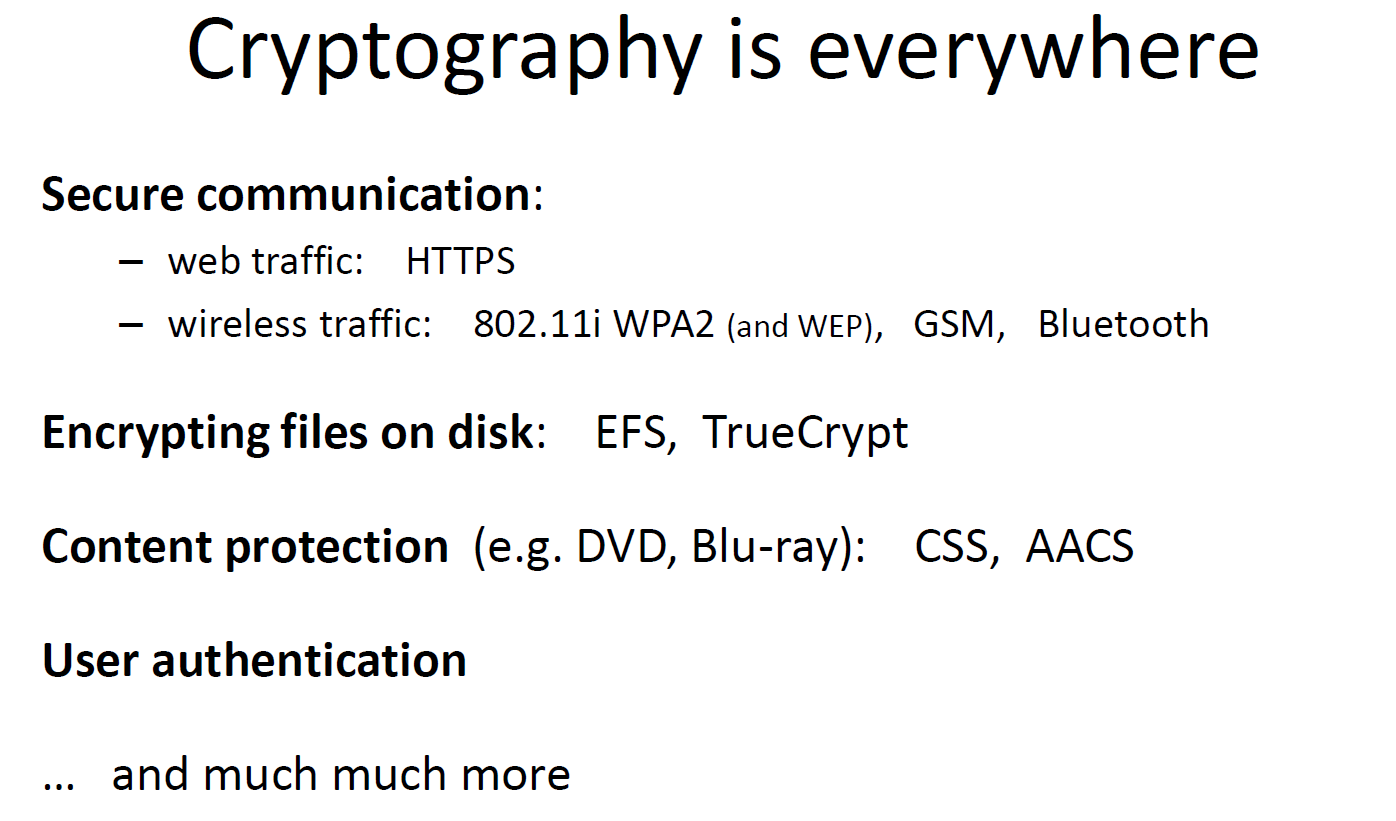
\includegraphics{./Images/CryptoIsEverywhere.png}

Cryptography prior to the modern age was effectively synonymous with
encryption, the conversion of information from a readable state to
apparent nonsense. The originator of an encrypted message shared the
decoding technique needed to recover the original information only with
intended recipients, thereby precluding unwanted persons from doing the
same. The cryptography literature often uses the name Alice (``A'') for
the sender, Bob (``B'') for the intended recipient, and Eve
(``eavesdropper'') for the adversary.

\textbf{History of Cryptography:} - Refer to the History segment inside
the following PDF:
Blockchain/CryptographyI/LectureSlides/Week1/Introduction.pdf -
\href{https://www.tutorialspoint.com/cryptography/origin_of_cryptography.htm}{History
of Cryptography} -
\href{https://www.tutorialspoint.com/cryptography/traditional_ciphers.htm}{Traditional
Ciphers: Substitution and Transposition}

Few Facts regarding Traditional Ciphers: - All of these systems are
based on symmetric key encryption scheme. - The only security service
these systems provide is confidentiality of information. - Unlike modern
systems which are digital and treat data as binary numbers, the earlier
systems worked on alphabets as basic element.

\textbf{Shifting from Traditional to Modern Cryptography: Product
Ciphers}

As we know, transposition cipher and substitution cipher by themselves
are vulnerable to cryptanalysis. However, using them in sequence and in
combinations can improve security, because the weakness of one cipher
can be masked or resolved by another cipher that is applied afterward.
Such use of combinations of substitution ciphers and transposition
ciphers is called product ciphers.

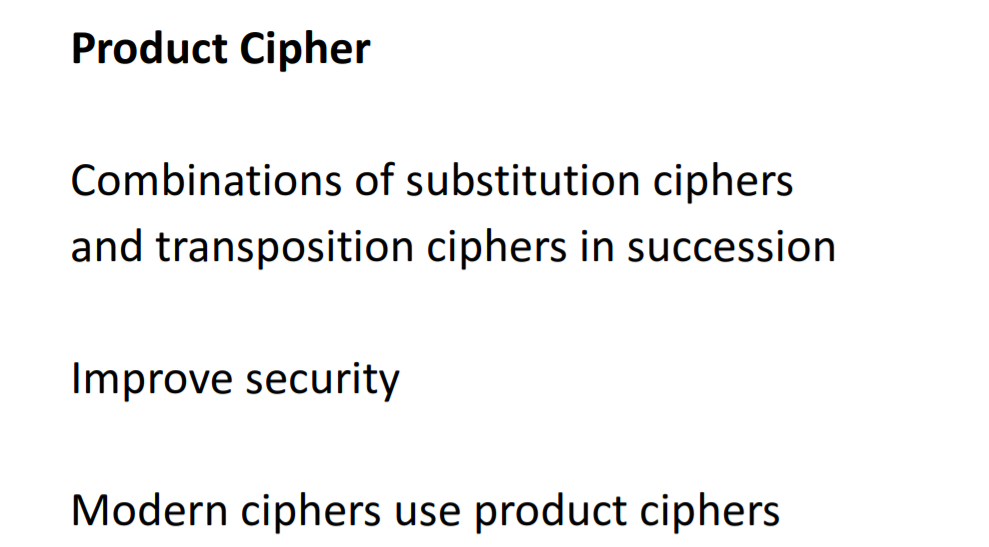
\includegraphics{./Images/ProductCiphers.png}

For example, while polyalphabetic substitution cipher can make the
frequency analysis more difficult (as compared to monoalphabetic
substitution ciphers) by making the frequency distribution more uniform.
It may still be subjected to a diagram or trigram-based cryptanalysis.
That is an attacker can look at a pair or triplet-based alphabets and
conduct a frequency analysis on those to infer the plaintext. Such
substitution cypher followed by a permutation cipher can be used to make
such sequence-based cryptanalysis more difficult. Because the
transposition cipher that follows makes the alphabets that used to be
adjacent to each other no longer adjacent to each other, because it
shuffles the ordering of the alphabets.

\begin{quote}
In contrast to classical ciphers, many practical modern substitution
ciphers use product ciphers to protect digital communications which are
often based on computer communications. And the use of product ciphers
is a key characteristic for modern ciphers. For example, popular
symmetric ciphers such as DES, data encryption standard, and AES,
Advanced Encryption Standards are based on product ciphers that
incorporates both substitution and transposition.
\end{quote}

\textbf{Modern Cryptography:} \textgreater{}Modern cryptography is
heavily based on mathematical theory and computer science practice;
\textbf{cryptographic algorithms are designed around computational
hardness assumptions}, making such algorithms hard to break in practice
by any adversary. It is theoretically possible to break such a system,
but it is infeasible to do so by any known practical means. These
schemes are therefore termed computationally secure; theoretical
advances, e.g., improvements in integer factorization algorithms, and
faster computing technology require these solutions to be continually
adapted. There exist \textbf{information-theoretically secure} schemes
that probably cannot be broken even with unlimited computing power---an
example is the one-time pad---but these schemes are more difficult to
implement than the best theoretically breakable but computationally
secure mechanisms.

More on:
\href{https://www.tutorialspoint.com/cryptography/modern_cryptography.htm}{Modern
Cryptography}

\textbf{Cryptology:} The art of devising ciphers (i.e cryptography) and
breaking them i.e., cryptanalysis) is collectively known as cryptology.

\textbf{Cryptanalysis:} Cryptanalysis is the study of analyzing
information systems in order to study the hidden aspects of the systems.
Cryptanalysis is used to breach cryptographic security systems and gain
access to the contents of encrypted messages, even if the cryptographic
key is unknown.

In addition to mathematical analysis of cryptographic algorithms,
cryptanalysis includes the study of side-channel attacks that do not
target weaknesses in the cryptographic algorithms themselves, but
instead exploit weaknesses in their implementation.

\begin{quote}
Cryptanalysis is the sister branch of Cryptography and they both
co-exist. The cryptographic process results in the cipher text for
transmission or storage. It involves the study of cryptographic
mechanism with the intention to break them. Cryptanalysis is also used
during the design of the new cryptographic techniques to test their
security strengths.
\end{quote}

\textbf{Kerckhoffs's Principle (also called Open Design or Shannon
Maxim):} \textgreater{}Kerckhoffs's principle is one of the basic
principles of modern cryptography. It was formulated in the end of the
nineteenth century by Dutch cryptographer Auguste Kerckhoffs. The
principle goes as follows: \textbf{A cryptographic system should be
secure even if everything about the system, except the key, is public
knowledge}. Basically, it implies that the attacker knows the
cryptographic system, i.e., the encryption and decryption schemes and
security relies on the secrecy of keys.

More on
\href{http://www.crypto-it.net/eng/theory/kerckhoffs.html}{Kerckhoffs's
Principle}.

\textbf{Steganography:} Steganography is the practice of
concealing/hiding a file, message, image, or video within another file,
message, image, or video. Steganography works on the principle of
\textbf{Security by Obscurity} (which is contrary to Kerckhoff's
Principle).

\textbf{The fundamental Parts of Cryptography: Crypto-Core}
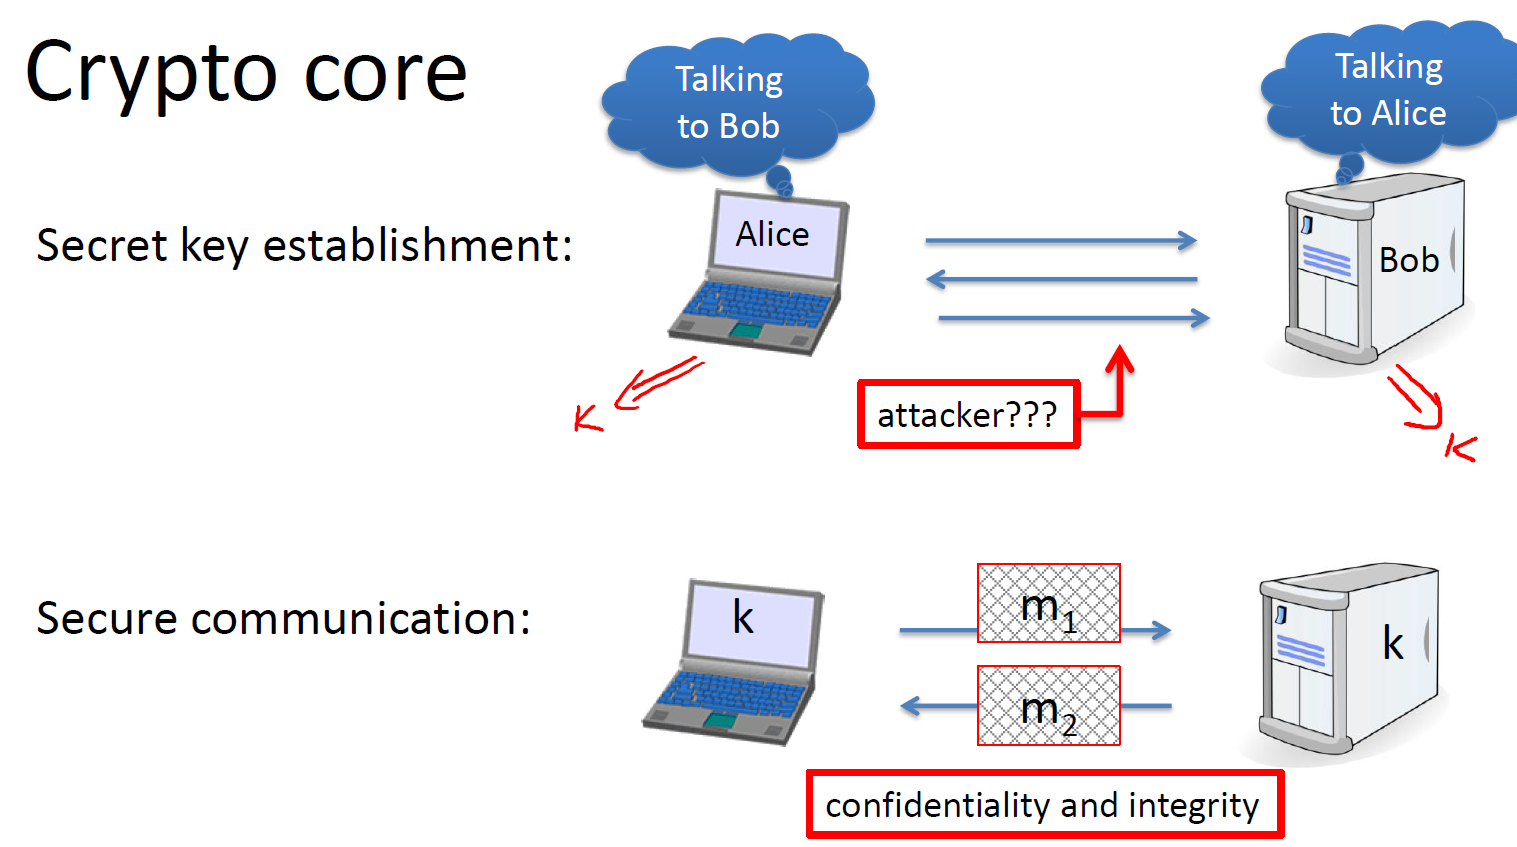
\includegraphics{./Images/CryptoCore.png}

Example: In context of the Secure Sockets Layer/Transport Layer
Security. 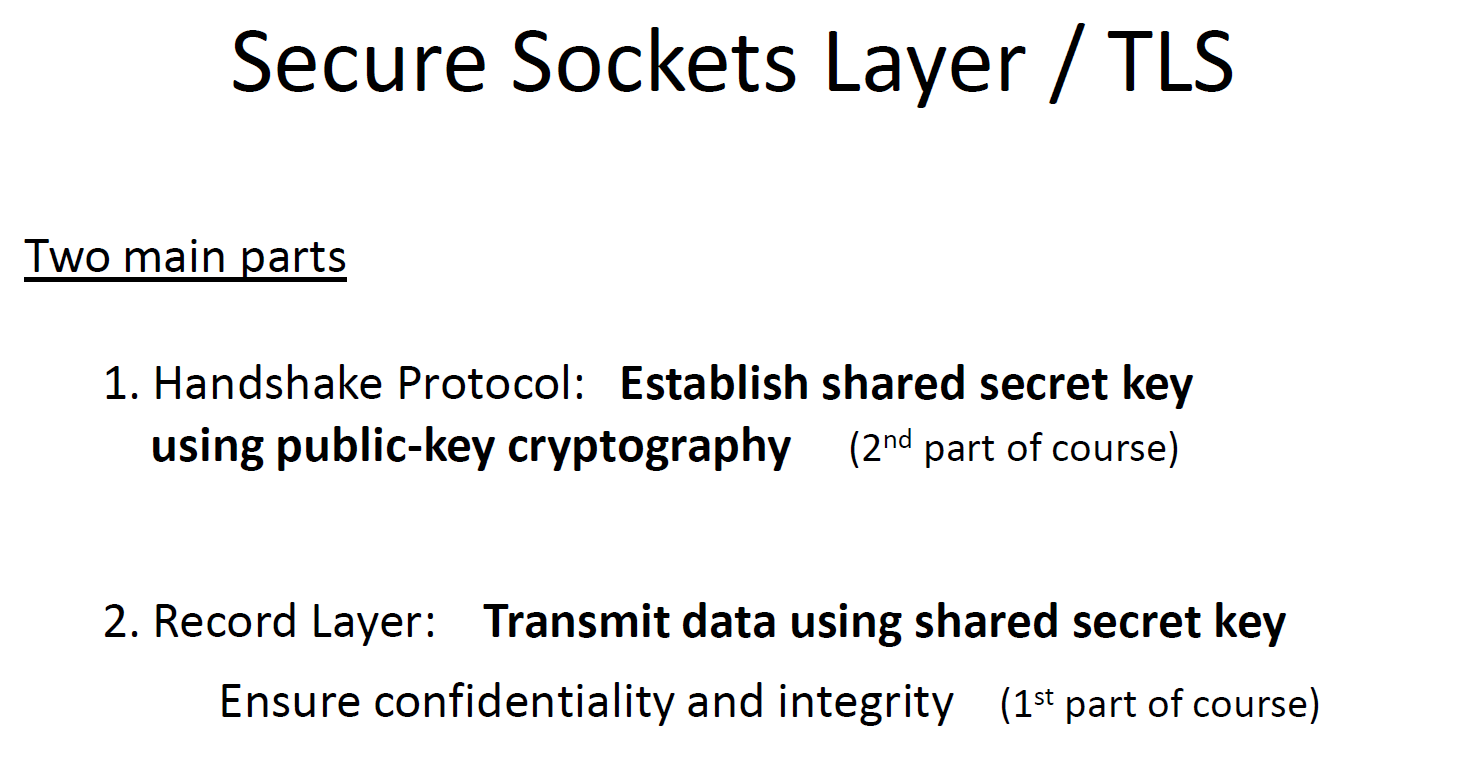
\includegraphics{./Images/TwoMainParts.png}

\textbf{Other Applications of Crypto} Beside key exchange and secure
communication, Cryptography can be used to do much more.

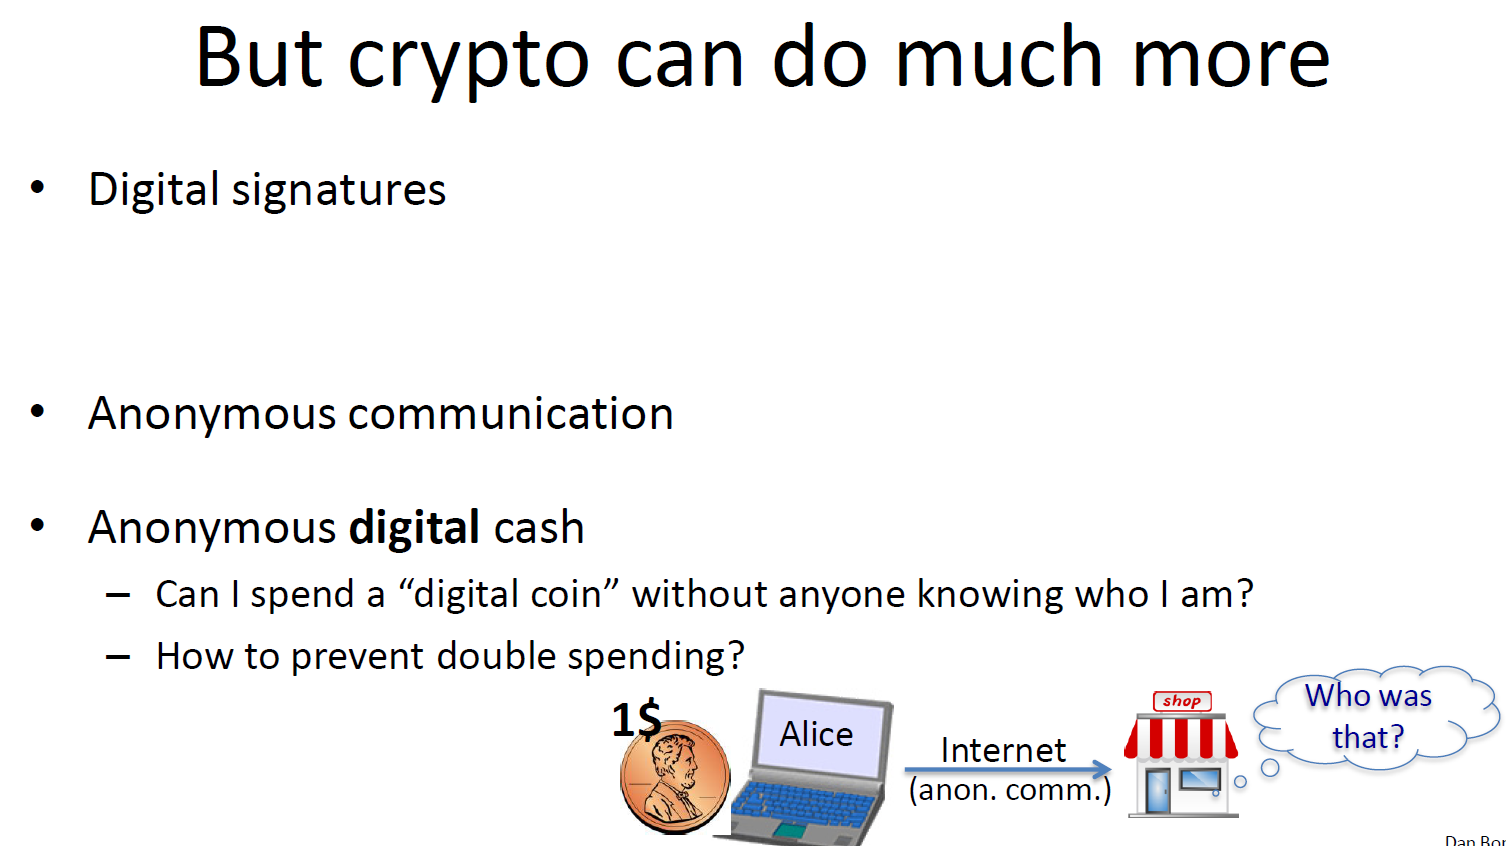
\includegraphics{./Images/MuchMoreViaCrypto.png}

Digital Signatures: - A digital signature, basically, is the analog of
the signature in the physical world. In the physical world, when you
sign a document, essentially, you write your signature on that document
and your signature is always the same. You always write the same
signature on all documents that you wanna sign. In the digital world,
this can't possibly work because if the attacker just obtained one
signed document from me, he can cut and paste my signature unto some
other document that I might not have wanted to sign. - And so, it's
simply not possible in a digital world that my signature is the same for
all documents that I want to sign. So we're gonna talk about how to
construct digital signatures in Cryptography II. It's really quite an
interesting primitive and we'll see exactly how build it. Just to give a
hint, the way digital signatures work is basically by making the digital
signature a function of the content being signed. So an attacker who
tries to copy my signature from one document to another is not gonna
succeed because the signature on the new document is not gonna be the
proper function of the data in the new document, and as a result, the
signature won't verify.

How Digital Signature Works (Intuition): - Imagine Alice wants to sign
some message m and send to Bob, what she would do first is she would
take the message, put it through the signing algorithm, where the
signing algorithm simply pushes the message into a hash function, say,
SHA-256 and generate a hash/digest/fingerprint (the value of the hash is
unique to the hashed data. Any change in the data, even changing or
deleting a single character, results in a different value.) and then it
would encrypt this hash using Alice's private/secret key and that's the
signing algorithm's output. - Alice then as usual encrypt the message
under Bob's public key and combine it with the output of the signing
algorithm. - Now Bob receives this combination of ciphertext with
encrypted hash, now what he does is, firstly he decrypt the message
using his private key. Once he decrypts and get the message m, he would
then use the verification algorithm to verify the signature. - The
verification algorithm would take message and the public key of Alice as
the input along with the encrypted hash. Now, it will take the message
and put it through the same hash algorithm as Alice did, SHA-256, and
generates the digest. And then it would use Alice's public key to
decrypt the received encrypted hash and compares both of the hash
values. - If the decrypted hash matches the now computed hash of the
data, it proves that the data hasn't changed since it was signed. If the
two hashes don't match, the data has either been tampered with in some
way (integrity) or the signature was created with a private key that
doesn't correspond to the public key presented by the signer
(authentication).

Anonymous Communication: - Imagine user Alice wants to talk to some chat
server, Bob. And, perhaps she wants to talk about a medical condition,
and so she wants to do that anonymously, so that the chat server doesn't
actually know who she is. Well, there's a standard method, called a
\textbf{mix net}, which is short for mix network, that allows Alice to
communicate over the public internet with Bob through a sequence of
proxies such that at the end of the communication Bob has no idea who he
just talked to. - The way mixnets work is basically as Alice sends her
messages to Bob through a sequence of proxies, these messages get
encrypted and decrypted appropriately so that Bob has no idea who he
talked to and the proxies themselves don't even know that Alice is
talking to Bob, or that actually who is talking to whom more generally.
One interesting thing about this anonymous communication channel is,
this is bi-directional. In other words, even though Bob has no idea who
he's talking to, he can still respond to Alice and Alice will get those
messages.

Once we have anonymous communication, we can build other privacy
mechanisms. And a good example of that is anonymous digital cash.

Anonymous Digital Cash: - As in the physical world if I have a physical
dollar, I can walk into a bookstore and buy a book and the merchant
would have no idea who I am. The question is whether we can do the exact
same thing in the digital world. - In the digital world, basically,
Alice might have a digital dollar, a digital dollar coin. And she might
wanna spend that digital dollar at some online merchants, perhaps some
online bookstore. Now, what we'd like to do is make it so that when
Alice spends her coin at the bookstore, the bookstore would have no idea
who Alice is. So we provide the same anonymity that we get from physical
cash. - Now the problem is that in the digital world, Alice can take the
one dollar coin that she had and can actually make copies of it. And
then all of a sudden instead of just having just one dollar coin now all
of a sudden she has three dollar coins and they're all the same of
course, and there's nothing preventing her from taking those replicas of
a dollar coin and spending it at other merchants. And so the question is
how do we provide anonymous digital cash but at the same time, also
prevent Alice from double spending the dollar coin at different
merchants? - In some sense there's a paradox here where anonymity is in
conflict with security because if we have anonymous cash there's nothing
to prevent Alice from double spending the coin and because the coin is
anonymous we have no way of telling who committed this fraud. And so the
question is how do we resolve this tension? And it turns out, it's
completely doable. Just to give a hint, I'll say that the way we do it
is basically by making sure that if Alice spends the coin once then no
one knows who she is, but if she spends the coin more than once i.e.~use
the coins replicas, all of a sudden, her identity is completely exposed
and then she could be subject to all sorts of legal problems.

\hypertarget{security-services-of-cryptography}{%
\subsubsection{Security Services of
Cryptography}\label{security-services-of-cryptography}}

The primary objective of using cryptography is to provide the following
\textbf{four fundamental information security services:}

\textbf{Confidentiality}

Confidentiality is the fundamental security service provided by
cryptography. It is a security service that keeps the information from
an unauthorized person. It is sometimes referred to as privacy or
secrecy.

Confidentiality can be achieved through numerous means starting from
physically securing to the use of mathematical algorithms for data
encryption.

\textbf{Data Integrity}

It is security service that deals with identifying any alteration to the
data. The data may get modified by an unauthorized entity intentionally
or accidentally. Integrity service confirms that whether data is intact
or not since it was last created, transmitted, or stored by an
authorized user.

Data integrity cannot prevent the alteration of data, but provides a
means for detecting whether data has been manipulated in an unauthorized
manner.

\textbf{Authentication}

Authentication provides the identification of the originator. It
confirms to the receiver that the data received has been sent only by an
identified and verified sender.

\begin{quote}
Authentication service has two variants: - Message authentication
identifies the originator of the message without any regard router or
system that has sent the message. - Entity authentication is assurance
that data has been received from a specific entity, say a particular
website.
\end{quote}

Apart from the originator, authentication may also provide assurance
about other parameters related to data such as the date and time of
creation/transmission.

\textbf{Non-repudiation}

It is a security service that ensures that an entity cannot refuse the
ownership of a previous commitment or an action. It is an assurance that
the original creator of the data cannot deny the creation or
transmission of the said data to a recipient or third party.

Non-repudiation is a property that is most desirable in situations where
there are chances of a dispute over the exchange of data. For example,
once an order is placed electronically, a purchaser cannot deny the
purchase order, if non-repudiation service was enabled in this
transaction.

\hypertarget{cryptography-primitives}{%
\subsubsection{Cryptography Primitives}\label{cryptography-primitives}}

Cryptographic primitives are well-established, low-level cryptographic
algorithms that are frequently used to build cryptographic protocols for
computer security systems. Alternatively, cryptography primitives can be
defined as the tools and techniques in Cryptography that can be
selectively used to provide a set of desired security services.

Following are some cryptography primitives: - Encryption - Hash
functions - Message Authentication codes (MAC) - Digital Signatures

When creating cryptographic systems, designers use cryptographic
primitives as their most basic building blocks. Because of this,
cryptographic primitives are designed to do one very specific task in a
highly reliable fashion.

The following table shows the primitives that can achieve a particular
security service on their own.

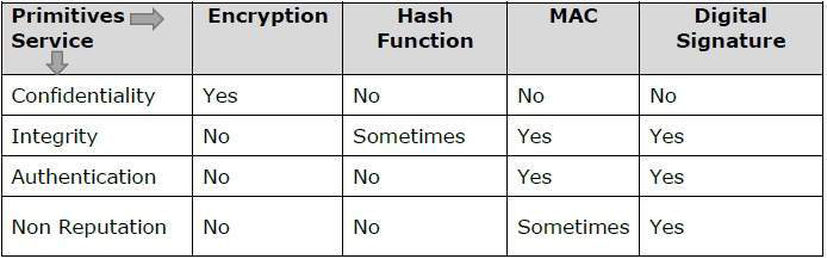
\includegraphics{./Images/CryptoPrimitives.png}

Note: Cryptographic primitives are intricately related and they are
often combined to achieve a set of desired security services from a
cryptosystem.

\hypertarget{the-three-fundamental-steps-in-cryptography}{%
\subsubsection{The three fundamental steps in
cryptography:}\label{the-three-fundamental-steps-in-cryptography}}

\begin{quote}
When we introduce/devise a new primitive these 3 steps have to be
rigorously followed: 1. \textbf{Precisely specify threat model:} Threat
model basically is knowing the capabilities of the adversaries, i.e.,
what can an adversarial do to attack the primitive and what is his goal
in forging the primitive. In order to show that the primitive or
cryptographic protocol is secure we need to prove that an adversary with
the following capabilities would not be able to break the
primitive/protocol. More on
\href{https://www.youtube.com/watch?v=f4tk2pnOUos}{Threat Model} 2.
\textbf{Propose a construction} 3. \textbf{Prove that breaking
construction under threat model will solve an underlying hard problem}:
A basic example would be, it is easy to multiply to large prime to get a
value N, but it's hard to recover the factors given the value N. So, if
our prime works on that concept than if an adversary breaks our
primitive/protocol than it would land a solution to solving that hard
problem.
\end{quote}

\textbf{Imp Note:} For production system usage, never ever use your own
implementation of the primitive or any cryptographic algorithm (as aside
from the implementation errors there could be many side channels which
could potentially result in easy breaching of your implementation). It
is always recommended to use a trusted library for applying ciphering to
production level data/information.
\href{https://www.youtube.com/watch?v=3Re5xlEjC8w}{Explanatory Video}

\begin{center}\rule{0.5\linewidth}{\linethickness}\end{center}

    \hypertarget{crash-course-on-discrete-probability}{%
\subsection{Crash Course on Discrete
Probability}\label{crash-course-on-discrete-probability}}

Reference Reads: - \textbf{Highly recommended (Easy to Digest read):}
\href{https://en.wikibooks.org/wiki/High_School_Mathematics_Extensions/Discrete_Probability}{Discrete
Probability} -
\href{http://www.henry.k12.ga.us/ugh/apstat/chapternotes/7supplement.html}{Discrete
vs Continuous Random Variables} -
\href{https://www.quora.com/What-is-the-difference-between-an-event-and-a-random-variable}{Random
Variable vs Events}

Reference Videos: -
\href{https://www.coursera.org/learn/crypto/lecture/qaEcL/discrete-probability-crash-course}{Discrete
Probability Crash Course {[}Part 1{]}} -
\href{https://www.coursera.org/learn/crypto/lecture/JkDRg/discrete-probability-crash-course-cont}{Discrete
Probability Crash Course {[}Part 2{]}} -
\href{https://www.youtube.com/watch?v=cqK3uRoPtk0}{Probability
Distribution for Random Variable X}

Why Discrete Probability? \textgreater{} Over the years many natural
cryptographic constructions were found to be insecure. In response,
modern cryptography was developed as a rigorous science where
constructions are always accompanied by a proof of security. The
language used to describe security relies on discreet probability.

Note: All the definitions given below are explained in context of
cryptography, as in crypto we mostly work around n-bit strings,
therefore the explanations for probabilistic concepts are provided while
keeping crypto as the central aspect.

\textbf{Probability Distribution}
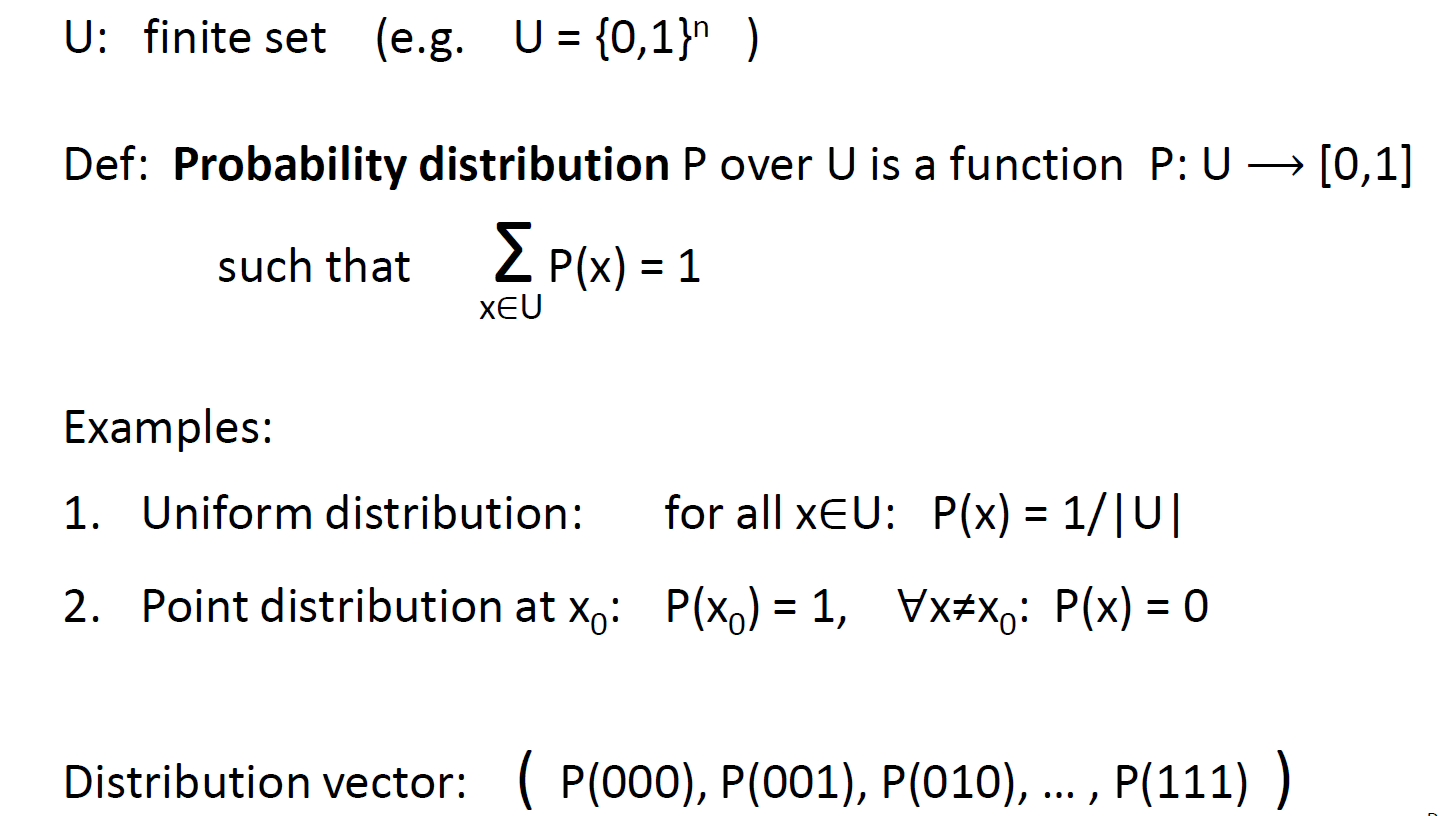
\includegraphics{./Images/ProbabilityDistribution.png}

Discrete probability is always defined over a universe which we'll
denote by U and this universe in our case is always going to be a finite
set. In fact very commonly our universe is going to be simply the set of
all n bit strings which here is denoted by \{0, 1\}\(^n\). Ex: \{0,
1\}\(^2\) is the set of all 2 bit string, that is, \{00, 01, 10, 11\}.
So there are 4 elements in this set and more generally there are \(2^n\)
elements in the set of n bits.

Now a probability distribution over this universe U is simply a function
which we'll denote by P, and this function, what it does, is it assigns
to every element in the universe a number between zero to one. And this
number is what's called the weight or the probability of that particular
element in the universe. Now there's only one requirement on this
function P, and that is that the sum of all the weights/probability, sum
up to one.

Classical Examples of Probability Distributions: - Uniform
Distribution:The uniform distribution assigns to every element in the
universe, exactly the same weight/probability. we are going to use
\textbar{}U\textbar{} to denote the size of the universe U. That is the
number of elements in the universe, and since we want the sum of all the
weights/probabilities to sum out to one, and we want all these weights
to be equal, what this means is that for every element x in the universe
U, we assign a probability of 1/\textbar{}U\textbar{}.\\
- Point Distribution at \(x_0\): What this point distribution does is
basically it puts all the weight on a single point, namely \(x_0\). So
here we assign to the point \(x_0\) all the weight/probability. And then
to all other points in the universe, we assign the weight zero.

Note: Because the universe U is going to be a finite set for us, we can
actually write down the weights that the distribution assigns to every
element in U, and represent the entire distribution as a vector. And the
size/dimension of vector would be the number of elements in the
distribution which is going to be \(2^n\), where n is the n-bit strings
that the Universe, \{0, 1\}\(^n\) is made up of.

\textbf{Events}

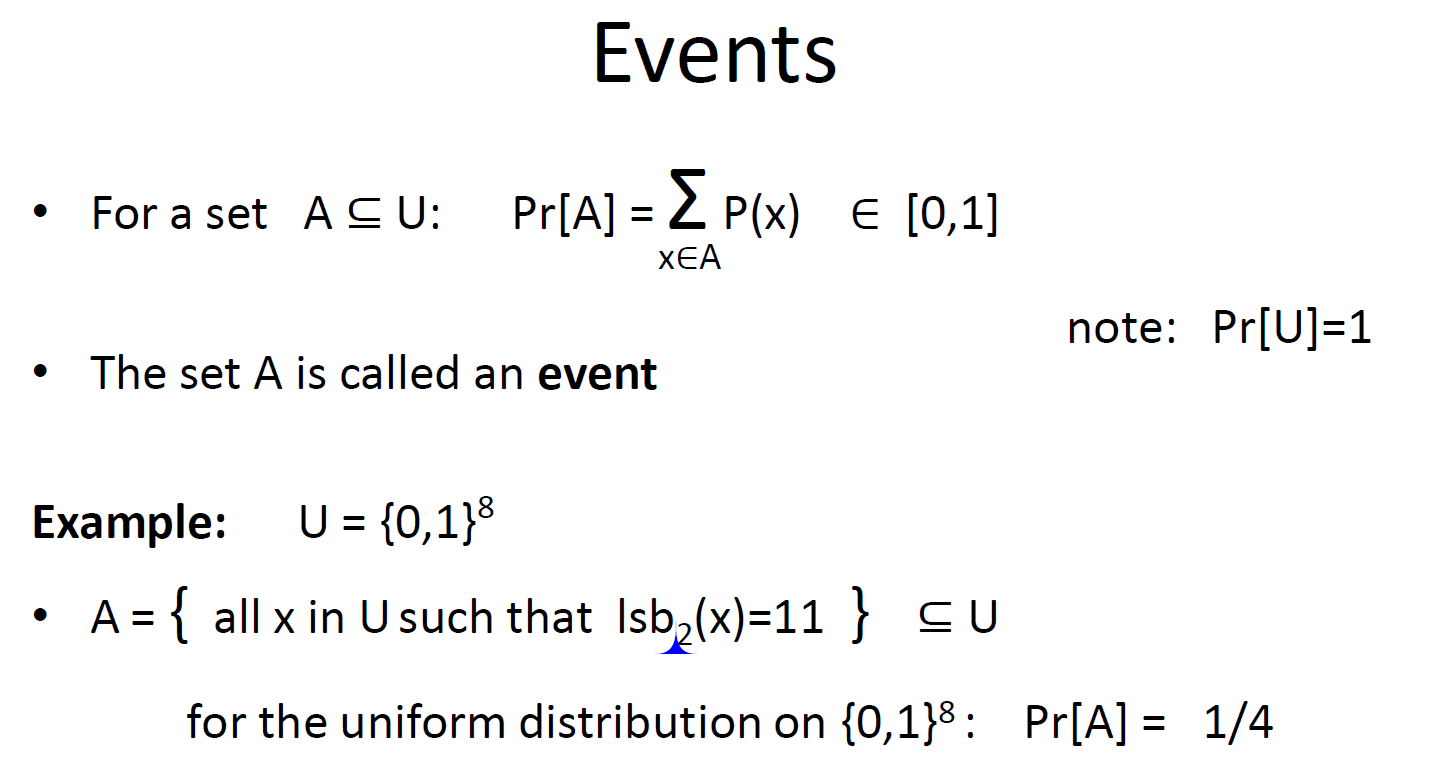
\includegraphics{./Images/Events.png}

Consider a subset A of our universe U. And we'll define the probability
of the subsets to be simply the sum of the weights of all the elements
in that subset. In other words, we're summing over all x in A, the
weights of these elements x in the set A. Now because the sum over the
entire universe of all weights needs to be one. This means that if we
look at the probability of a subset of the universe, we're gonna get
some number in the interval zero to one. So, a subset A of the universe
U is called an event. And the probability of the set A is called the
probability of that event.

So let's look at a simple example: - Suppose we look at the universe U,
which consists of all 8-bit strings, therefore, the size of this
universe U is \(2^8\) which is 256 strings. Essentially we're looking at
all byte values, all 256 possible byte values. - Now let's define the
following event A. Basically the event is gonna contain all bytes so all
8-bit strings in the universe such that the two least significant bits
of the byte happens to be 1, that is, the strings that end with 11. -
And now let's look at the uniform distribution over the universe U and
think what is the probability of the event A? So what is the probability
that when we choose a random byte, the two least significant bits of
that byte happens to be one, one? - Well the answer is one-fourth, and
the reason that's true is because it's not too difficult to convince
yourself that of in the 256 eight bit strings, exactly 64 of them, one
quarter of them, end in 11. And as we're looking at the uniform
distribution, hence the probability of each string is exactly one over
the size of the universe, mainly 1/256. And the product of 64 elements
of the event A with the probability of each element 1/256 yields the
probability equal to one-fourth, which is the probability of the event A
that we're looking at.

\textbf{Union Bound}

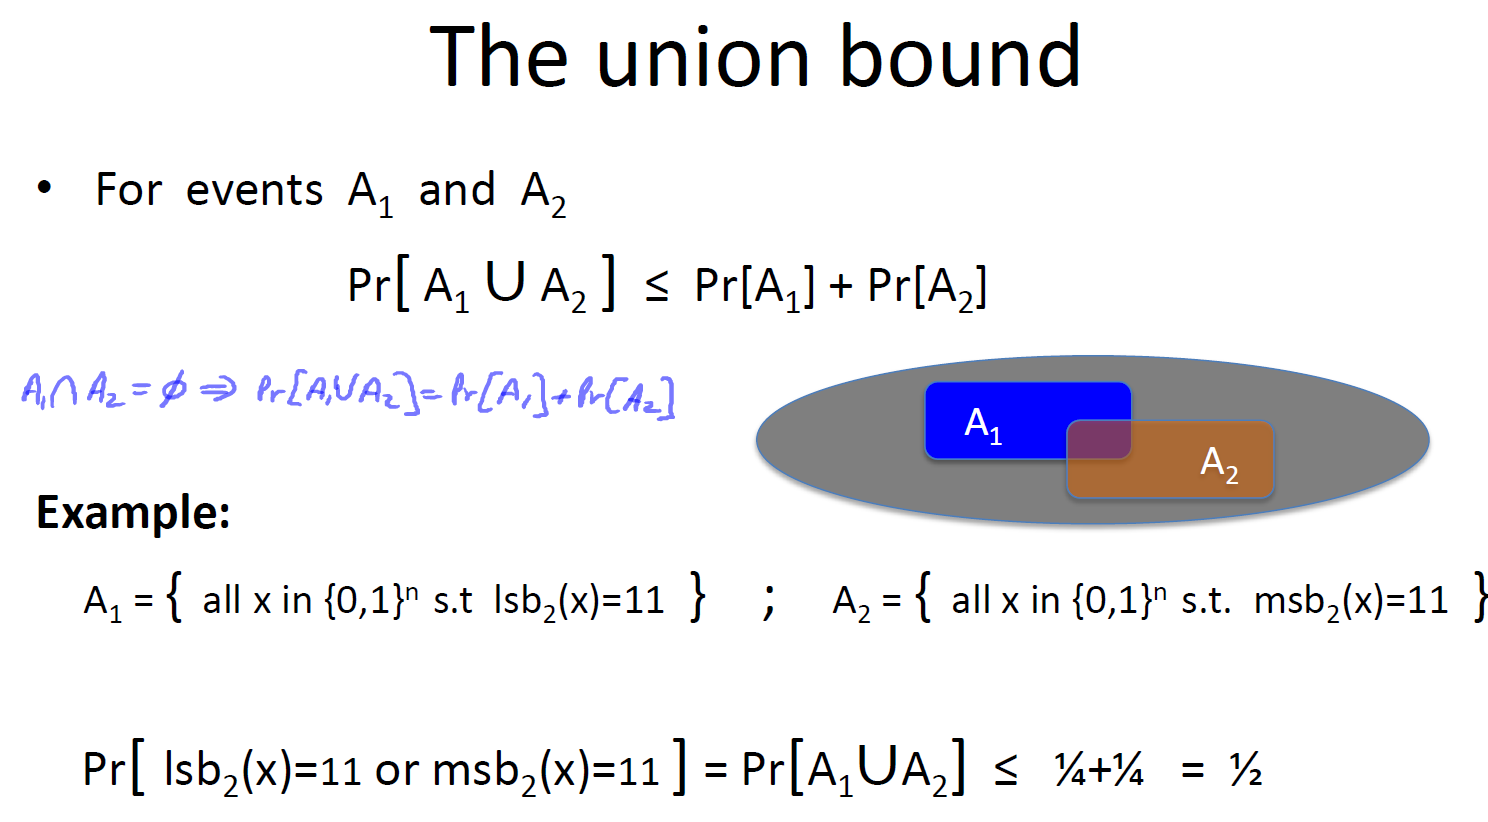
\includegraphics{./Images/UnionBound.png}

A very simple bound on the probability of events is called the union
bound. Imagine we have two events A1 and A2. So these are both subsets
of some universe U and we wanna know what is the probability that either
A1 occurs, or A2 occurs In other words, what is the probability of the
union of these two events? The A1 U A2 denotes the union of the two
sets. So the union bound tells us that the probability that either A1
occurs or A2 occurs is basically less than the sum of the two
probabilities. And that's actually quite easy to see. So simply look at
this picture, we can see that when we look at, at the sum of the two
probabilities, we're basically summing the probability of all the
elements in A1, all the elements in A2. And we realize that we kind of
double-summed these elements in the intersection.

If the two events are disjoint, in other words they're intersection is
empty, in that case if we look at the sum of the probability that either
A1 or A2 happens, that's exactly equal to the sum of the two
probabilities.

Formulas: Intersection: - When A and B are independent events (event A
simply tells nothing about event B): P(A \(\cap\) B) = P(A).P(B) - When
A and B are dependent, then we use what's called conditional
probability: P(A \(\cap\) B) = P(A).P(B\textbar{}A) =
P(B).P(A\textbar{}B). Note: The probability that Event A occurs, given
that Event B has occurred, is called a conditional probability. The
conditional probability of Event A, given Event B, is denoted by the
symbol P(A\textbar{}B).

Union: P(A \(\cup\) B) = P(A) + P(B) - P(A \(\cap\) B), for disjoint
events P(A \(\cap\) B) = 0, then P(A \(\cup\) B) = P(A) + P(B)

\textbf{Random Variables}

Random variables are fairly intuitive objects. But unfortunately the
formal definition of a random variable can be a little confusing. So, we
will supplement it with an example, and hopefully that will be clear
enough. So formally, a random variable denoted by X is a function, from
the universe U into some set V and we say that this set V is where the
random variable takes its values.

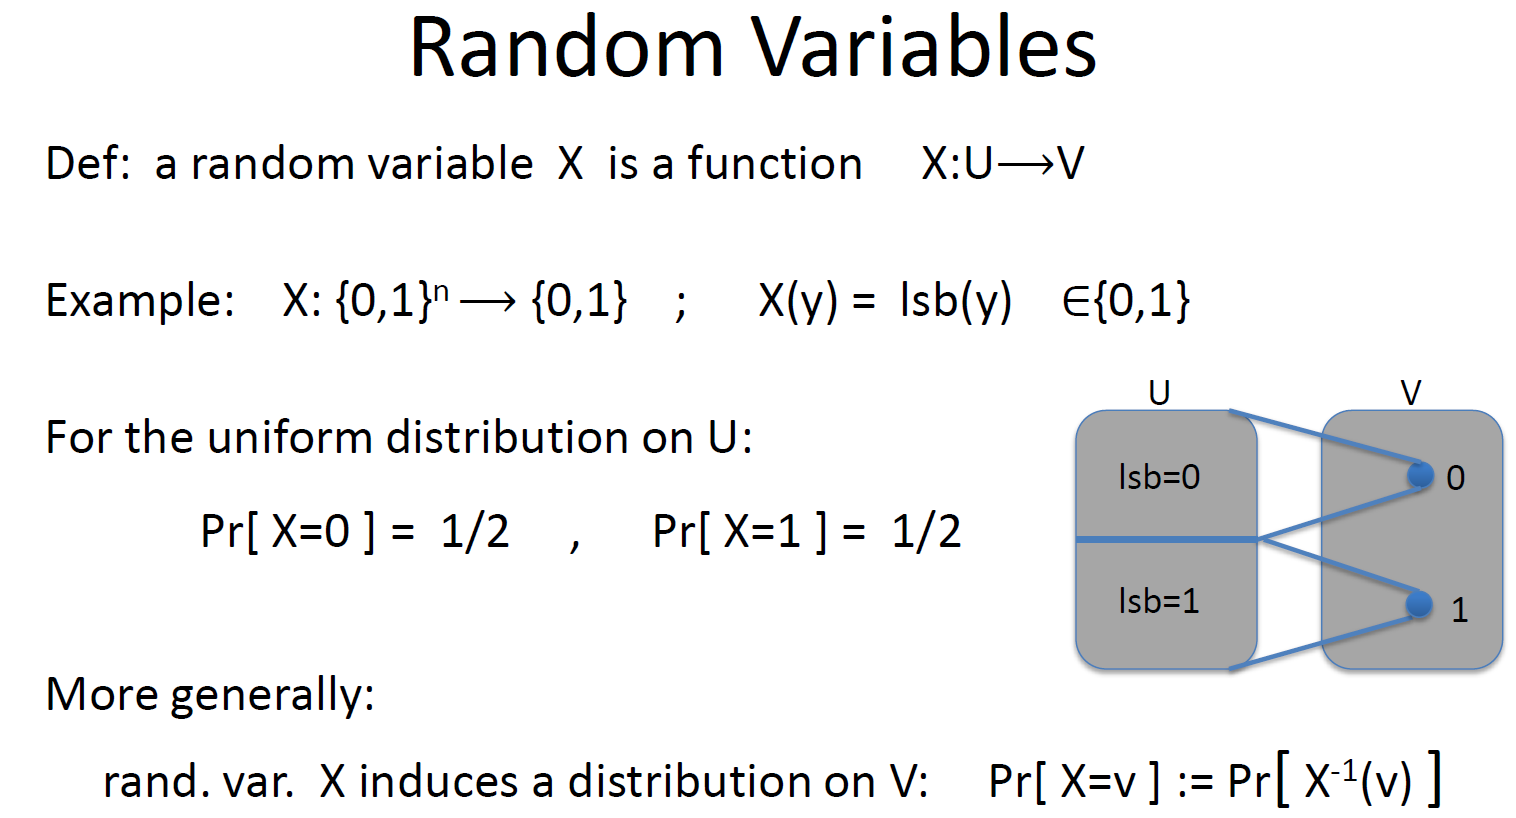
\includegraphics{./Images/RandomVariables.png}

Let's look at a particular example: - Suppose we have a random variable
X And this random variable maps a the universe \{0, 1\}\(^n\) into the
set \{0, 1\}. So the values of this random variable are going to be
either zero or one. So, that values in this case will be of one bit. -
Now, this random variable maps our universe, which is the center of all
n-bit binary strings. How does it do it? Well, given a particular sample
in the universe, a particular n-bit string y. What the random variable
will do is simply output the least significant bit of y And that's it,
that is, X(y) outputs the least significant bit. That's the whole random
variable. - Suppose we look at a uniform distribution on the set \{0,
1\}\(^n\). Let me ask you what is the probability that this random
variable to output zero and what is the probability that the random
variable outputs one? Well we can see that the answers are 1/2 and 1/2.
- Why so? Because the Universe has a uniform distribution which
essentially means that it has equal probability to output an n-bit
string which ends with 0 vs the ones which ends with 1. So the
probability that the random variable outputs 0 or 1 is 50:50.

Now, more generally, if we have a random variable defined on a universe
U and is taking values in a certain set V, then this random variable
actually induces a probability distribution on this set V i.e.~the
elements in the set V have certain probabilities attached to them, in
other words, for each element in V it assigns some probability/weight to
each of them.

Uniform Random Variable 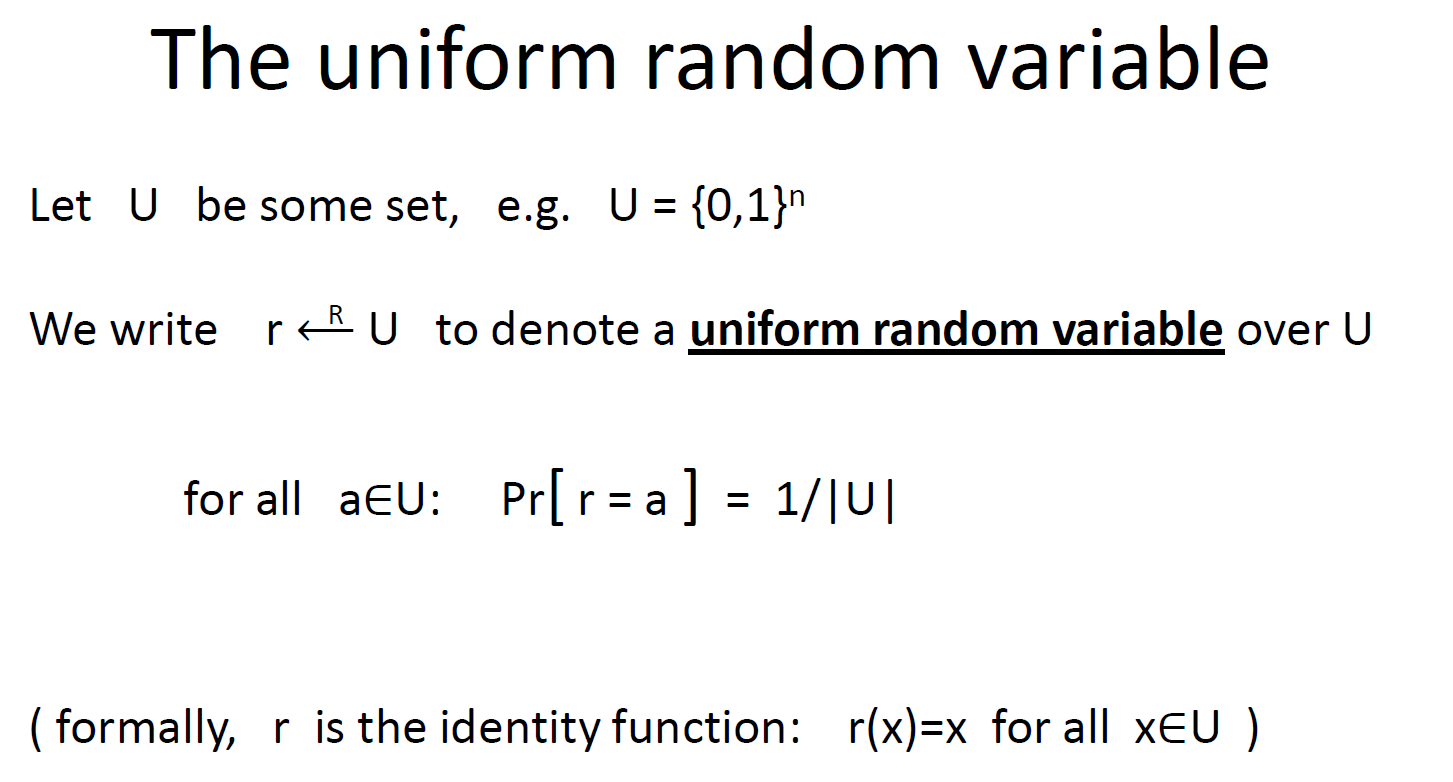
\includegraphics{./Images/UniformRandVar.png}
We're gonna denote a random variable R that basically sample's uniformly
from the set U by a little arrow with a R on top of it, where r is the
value that the uniform random variable R produced. Notice that the
random variable R is literally a uniform random variable sampled over
the set U. So in symbols what's this means is that for all elements a in
the universe, the probability that r = a is simply
1/\textbar{}U\textbar{}.

Formal Definition: Formally, the uniform random variable is an identity
function namely r(x) is equal to x for all x in the universe U.

\textbf{Randomized Algorithms:}

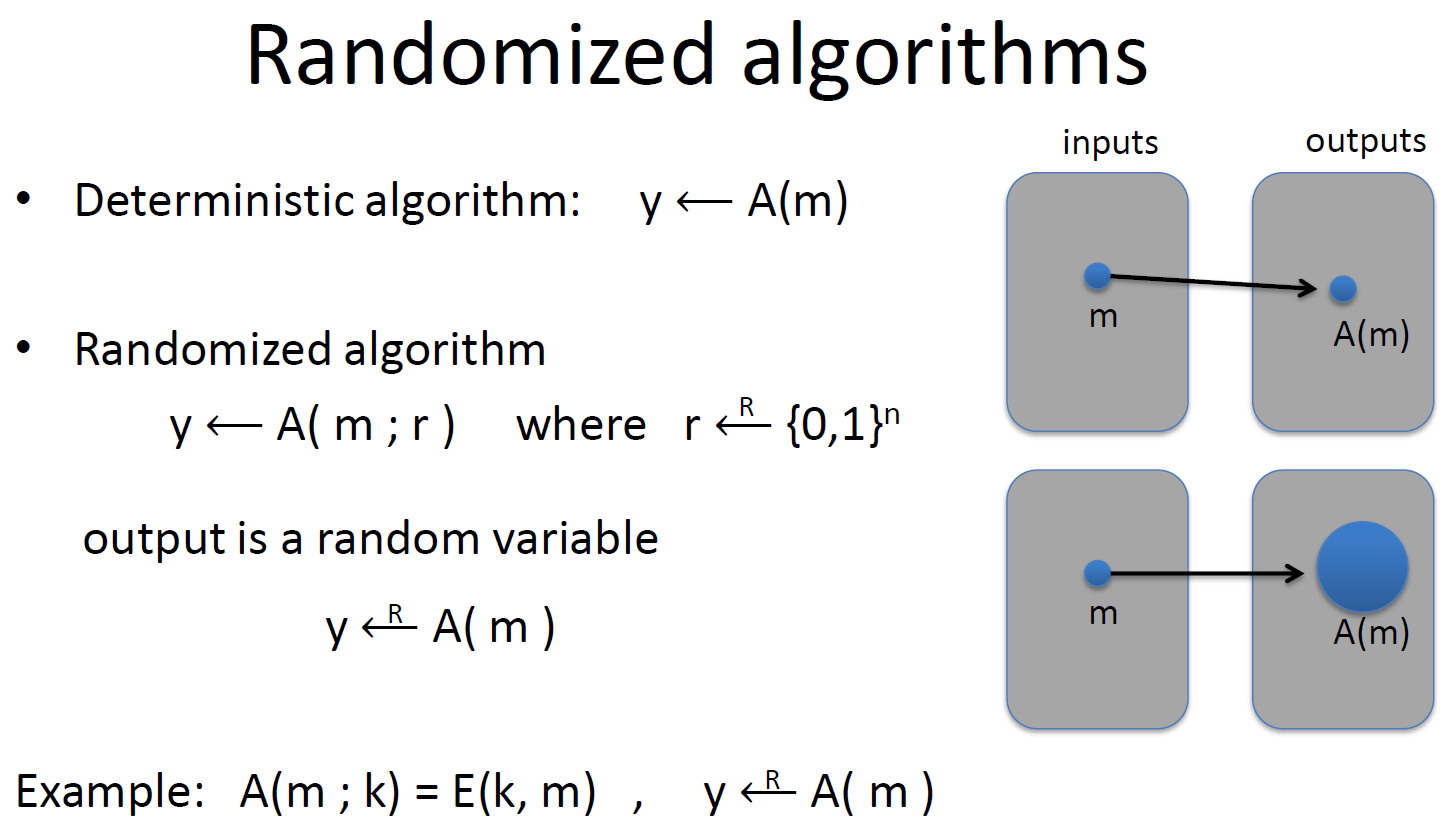
\includegraphics{./Images/RandomAlgs.png}

It's due to Discrete Probability that cryptographic algorithms took a
leap from being deterministic in nature, producing same output for a
given input each time, to being randomized algorithms that we use today.

Randomized Algorithms are those which produce different outputs given
the same input, i.e., even though the input to the randomized algorithm
is the same, it will produce different output each time, as Random
Algorithm have an implicit argument, say r, which is uniformly sampled
anew, from it's given universe, every time the algorithm is run,
therefore making the outcome different.

The output of this Random Algorithm is basically a random variable, say
y, which is a distribution over the set of all possible encryption of
message m under a uniform key r. So the main point to remember is that
even though the inputs to a randomized algorithm might always be the
same every time you run the randomized algorithm you're gonna get a
different output.

\textbf{XOR {[}Exclusive-OR{]}} XOR is very important when it comes to
cryptography. Review: XOR of two bit string is their bitwise addition
mod 2. Also, something XORed with itself yields zeros, that is, xxx XOR
xxx yields 0. For ex: 101011 XOR 101011 = 000000.

An Important Property of XOR:
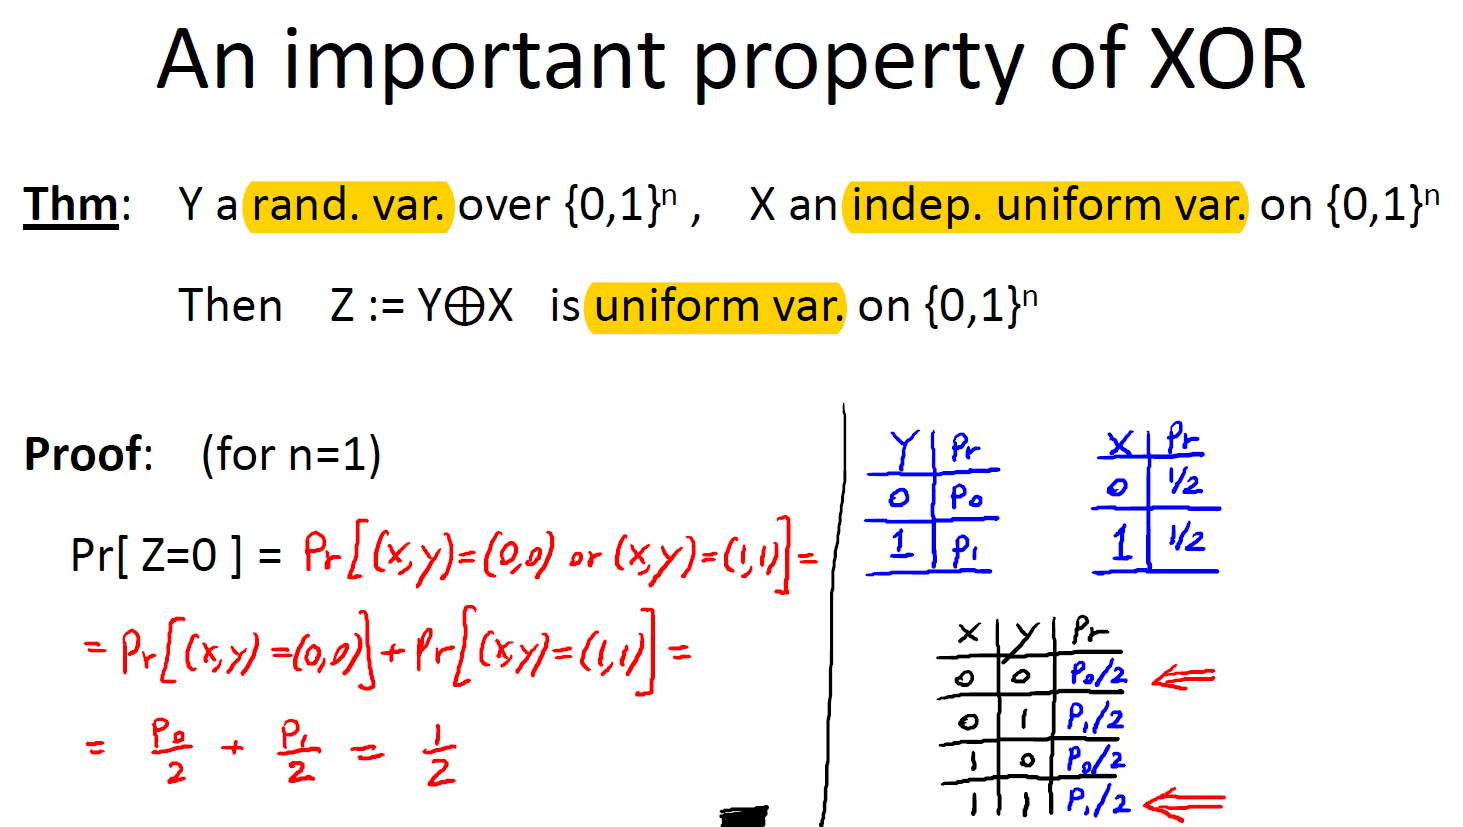
\includegraphics{./Images/XOR-Property.png}

The property is as follows: Suppose we have a random variable Y that's
distributed arbitrarily over \{0, 1\}\(^n\). So we know nothing about
the distribution of Y. But now, suppose we have an independent random
variable X that happens to be uniformly distributed also over \{0,
1\}\(^n\). So it's very important that X is uniform and is independent
of Y. So now let's define the random variable Z which is the XOR of X
and Y. Then we can claim that no matter what distribution Y started
with, the distribution Z is always going to be a uniform random
variable.

In other words if we take an arbitrarily malicious distribution and we
XOR it with independent uniform random variable what we end up with is a
uniform random variable. Note: This is kind of a key property that makes
XOR very useful for crypto.

For explanation regarding the proof, that is shown in the image above,
of the imp property of XOR please tune into to the following video
\href{https://www.coursera.org/learn/crypto/lecture/JkDRg/discrete-probability-crash-course-cont}{Discrete
Probability Crash Course {[}Part 2{]}} at 7:25.

\begin{center}\rule{0.5\linewidth}{\linethickness}\end{center}

    \hypertarget{cryptosystems}{%
\subsection{Cryptosystems}\label{cryptosystems}}

A cryptosystem is an implementation of cryptographic techniques and
their accompanying infrastructure to provide information security
services. A cryptosystem is also referred to as a cipher system.

\hypertarget{components-of-a-cryptosystem}{%
\subsubsection{Components of a
Cryptosystem}\label{components-of-a-cryptosystem}}

The various components of a basic cryptosystem are as follows:

\begin{itemize}
\item
  \textbf{Plaintext:} It is the data to be protected during
  transmission.
\item
  \textbf{Encryption Algorithm:} It is a mathematical process that
  produces a ciphertext for any given plaintext and encryption key. It
  is a cryptographic algorithm that takes plaintext and an encryption
  key as input and produces a ciphertext.
\item
  \textbf{Ciphertext:} It is the scrambled version of the plaintext
  produced by the encryption algorithm using a specific the encryption
  key. The ciphertext is not guarded. It flows on public channel. It can
  be intercepted or compromised by anyone who has access to the
  communication channel.
\item
  \textbf{Decryption Algorithm:} It is a mathematical process, that
  produces a unique plaintext for any given ciphertext and decryption
  key. It is a cryptographic algorithm that takes a ciphertext and a
  decryption key as input, and outputs a plaintext. The decryption
  algorithm essentially reverses the encryption algorithm and is thus
  closely related to it.
\item
  \textbf{Encryption Key:} It is a value that is known to the sender.
  The sender inputs the encryption key into the encryption algorithm
  along with the plaintext in order to compute the ciphertext.
\item
  \textbf{Decryption Key:} It is a value that is known to the receiver.
  The decryption key is related to the encryption key, but is not always
  identical to it. The receiver inputs the decryption key into the
  decryption algorithm along with the ciphertext in order to compute the
  plaintext.
\end{itemize}

For a given cryptosystem, a collection of all possible decryption keys
is called a \textbf{key space}.

An interceptor (an attacker) is an unauthorized entity who attempts to
determine the plaintext. He can see the ciphertext and may know the
decryption algorithm. He, however, must never know the decryption key.

\hypertarget{types-of-cryptosystems}{%
\subsubsection{Types of Cryptosystems}\label{types-of-cryptosystems}}

Fundamentally, there are two types of cryptosystems based on the manner
in which encryption-decryption is carried out in the system:

\begin{itemize}
\tightlist
\item
  Symmetric Key Cryptosystems
\item
  Asymmetric Key Cryptosystems
\end{itemize}

The main difference between these cryptosystems is the relationship
between the encryption and the decryption key. Logically, in any
cryptosystem, both the keys are closely associated. It is practically
impossible to decrypt the ciphertext with the key that is unrelated to
the encryption key.

\hypertarget{cryptographic-attacks}{%
\subsubsection{Cryptographic Attacks}\label{cryptographic-attacks}}

The basic intention of an attacker is to break a cryptosystem and to
find the plaintext from the ciphertext. To obtain the plaintext, the
attacker only needs to find out the secret decryption key, as the
algorithm is already in public domain.

Hence, he applies maximum effort towards finding out the secret key used
in the cryptosystem. Once the attacker is able to determine the key, the
attacked system is considered as broken or compromised.

Based on the methodology used, attacks on cryptosystems are categorized
as follows:

\begin{itemize}
\item
  \textbf{Ciphertext Only Attacks (COA):} In this method, the attacker
  has access to a set of ciphertext(s). He does not have access to
  corresponding plaintext. COA is said to be successful when the
  corresponding plaintext can be determined from a given set of
  ciphertext. Occasionally, the encryption key can be determined from
  this attack. Modern cryptosystems are guarded against ciphertext-only
  attacks.
\item
  \textbf{Known Plaintext Attack (KPA):} In this method, the attacker
  knows the plaintext for some parts of the ciphertext. The task is to
  decrypt the rest of the ciphertext using this information. This may be
  done by determining the key or via some other method. The best example
  of this attack is linear cryptanalysis against block ciphers.
\item
  \textbf{Chosen Plaintext Attack (CPA):} In this method, the attacker
  has the text of his choice encrypted. So he has the
  ciphertext-plaintext pair of his choice. This simplifies his task of
  determining the encryption key. An example of this attack is
  differential cryptanalysis applied against block ciphers as well as
  hash functions. A popular public key cryptosystem, RSA is also
  vulnerable to chosen-plaintext attacks.
\item
  \textbf{Dictionary Attack:} This attack has many variants, all of
  which involve compiling a `dictionary'. In simplest method of this
  attack, attacker builds a dictionary of ciphertexts and corresponding
  plaintexts that he has learnt over a period of time. In future, when
  an attacker gets the ciphertext, he refers the dictionary to find the
  corresponding plaintext.
\item
  \textbf{Brute Force Attack/Extensive Search:} In this method, the
  attacker tries to determine the key by attempting all possible keys.
  If the key is 8 bits long, then the number of possible keys is 28 =
  256. The attacker knows the ciphertext and the algorithm, now he
  attempts all the 256 keys one by one for decryption. The time to
  complete the attack would be very high if the key is long.
\item
  \textbf{Birthday Attack:} This attack is a variant of brute-force
  technique. It is used against the cryptographic hash function. When
  students in a class are asked about their birthdays, the answer is one
  of the possible 365 dates. Let us assume the first student's birthdate
  is 3rd Aug.~Then to find the next student whose birthdate is 3rd Aug,
  we need to enquire 1.25*√365 ≈ 25 students. Similarly, if the hash
  function produces 64 bit hash values, the possible hash values are
  1.8x10\^{}19. By repeatedly evaluating the function for different
  inputs, the same output is expected to be obtained after about
  5.1x10\^{}9 random inputs. If the attacker is able to find two
  different inputs that give the same hash value, it is a collision and
  that hash function is said to be broken.
\item
  \textbf{Man in Middle Attack (MIM):} The targets of this attack are
  mostly public key cryptosystems where key exchange is involved before
  communication takes place.

  \begin{itemize}
  \tightlist
  \item
    Host A wants to communicate to host B, hence requests public key of
    B.
  \item
    An attacker intercepts this request and sends his public key
    instead.
  \item
    Thus, whatever host A sends to host B, the attacker is able to read.
  \item
    In order to maintain communication, the attacker re-encrypts the
    data after reading with his public key and sends to B.
  \item
    The attacker sends his public key as A's public key so that B takes
    it as if it is taking it from A.
  \end{itemize}
\item
  \textbf{Side Channel Attack (SCA):} This type of attack is not against
  any particular type of cryptosystem or algorithm. Instead, it is
  launched to exploit the weakness in physical implementation of the
  cryptosystem. They map things like the time taken for encryption or
  the power consumed during encryption to deduce the key.
\item
  \textbf{Timing Attacks:} They exploit the fact that different
  computations take different times to compute on processor. By
  measuring such timings, it is be possible to know about a particular
  computation the processor is carrying out. For example, if the
  encryption takes a longer time, it indicates that the secret key is
  long.
\item
  \textbf{Power Analysis Attacks:} These attacks are similar to timing
  attacks except that the amount of power consumption is used to obtain
  information about the nature of the underlying computations.
\item
  \textbf{Fault analysis Attacks:} In these attacks, errors are induced
  in the cryptosystem and the attacker studies the resulting output for
  useful information.
\end{itemize}

\begin{center}\rule{0.5\linewidth}{\linethickness}\end{center}

    \hypertarget{symmetric-key-cryptosystems}{%
\subsection{Symmetric Key
Cryptosystems}\label{symmetric-key-cryptosystems}}

The encryption process where \textbf{same keys are used for encrypting
and decrypting} the information is known as Symmetric Key Encryption.
The study of symmetric cryptosystems is referred to as symmetric
cryptography. Symmetric cryptosystems are also sometimes referred to as
\textbf{secret key cryptosystems}.

A few well-known examples of symmetric key encryption methods are:
Digital Encryption Standard (DES), Triple-DES (3-DES), IDEA, RC4,
eStreams and BLOWFISH.
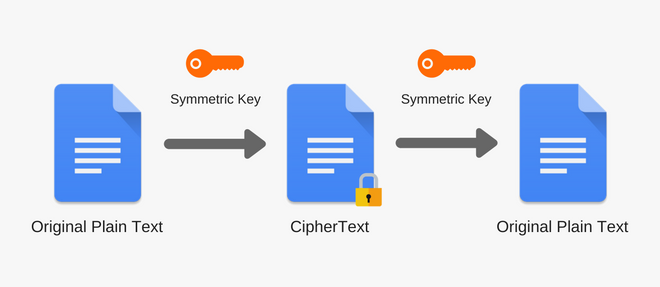
\includegraphics{./Images/SymmetricEncryption.png}

\textbf{Crypto Lesson:} In a symmetric cryptosystem, you should never
use a single shared key to encrypt data/information in both direction
i.e.~traffic from Client(C) to Sever(S) should not be encrypted with the
same key as used for encrypting the traffic from Server to Client.
Hence, the shared key should be a pair of keys =\textgreater{}
\(K_{shared}\) = \{\(K_{C>>S}\), \(K_{S>>C}\)\} where prior is used to
encrypt/decrypt the information from client to server and the latter
from server to client.

\textbf{Symmetric Ciphers:}
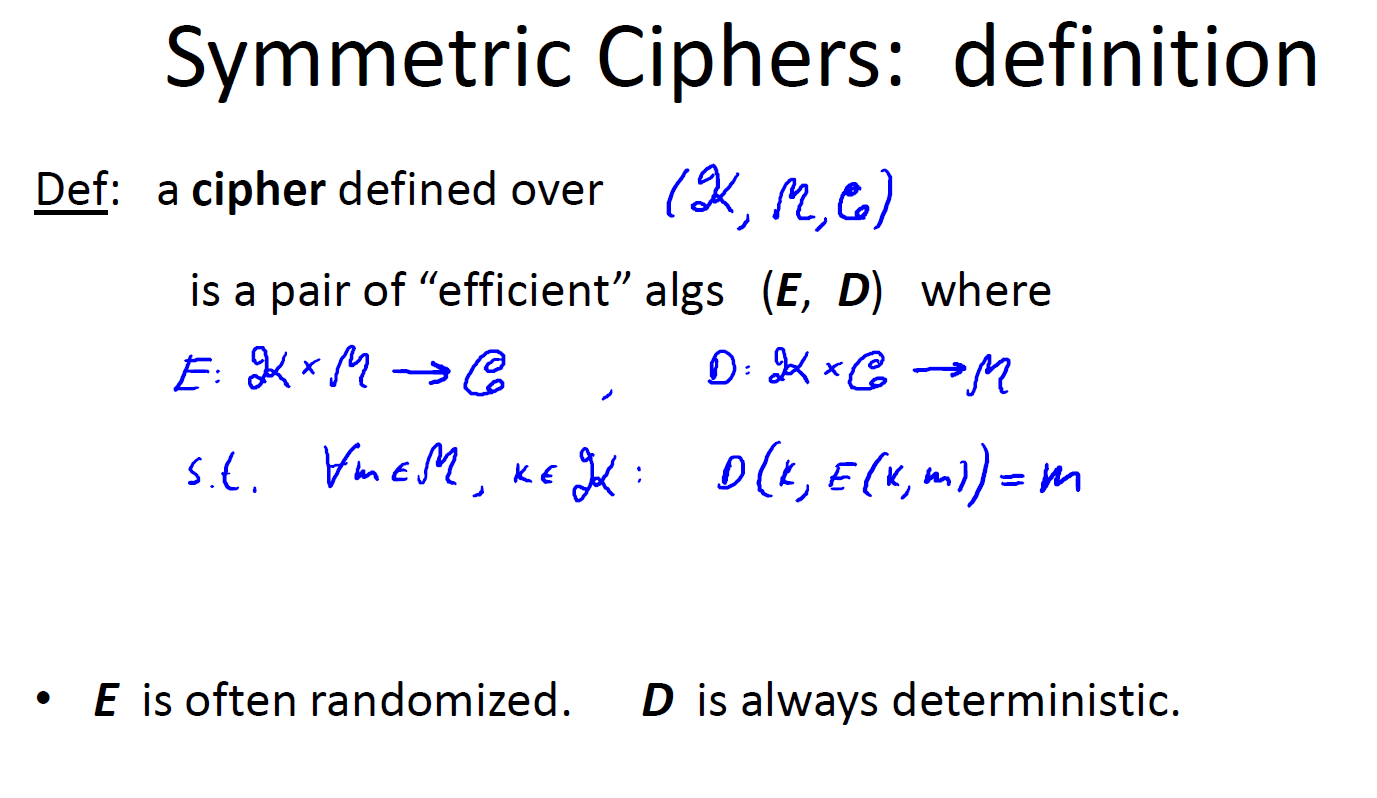
\includegraphics{./Images/SymmetricCipherDef.png}

\textbf{Type of symmetric ciphers:} An important distinction in
symmetric cryptographic algorithms is between stream and block ciphers.
- \textbf{Section \ref{stream-ciphers}} convert one symbol of plaintext
directly into a symbol of ciphertext. -
\textbf{Section \ref{block-ciphers}} encrypt a group of plaintext
symbols as one block.

Prior to 1970, all cryptosystems employed symmetric key encryption. Even
today, its relevance is very high and it is being used extensively in
many cryptosystems. It is very unlikely that this encryption will fade
away, as it has certain advantages over asymmetric key encryption.

The \textbf{salient features of cryptosystem based on symmetric key
encryption} are: - Persons using symmetric key encryption must share a
common key prior to exchange of information. - Keys are recommended to
be changed regularly to prevent any attack on the system. - A robust
mechanism needs to exist to exchange the key between the communicating
parties. As keys are required to be changed regularly, this mechanism
becomes expensive and cumbersome. - In a group of n people, to enable
two-party communication between any two persons, the number of keys
required for group is \(\frac{n\times (n-1)}{2}\). - Length of Key
(number of bits) in this encryption is smaller and hence, process of
encryption-decryption is faster than asymmetric key encryption. -
Processing power of computer system required to run symmetric algorithm
is less.

\textbf{Challenge of Symmetric Key Cryptosystem} There are two
restrictive challenges of employing symmetric key cryptography:

\begin{itemize}
\item
  \textbf{Key establishment:} Before any communication, both the sender
  and the receiver need to agree on a secret symmetric key. It requires
  a secure key establishment mechanism in place.
\item
  \textbf{Trust Issue:} Since the sender and the receiver use the same
  symmetric key, there is an implicit requirement that the sender and
  the receiver `trust' each other. For example, it may happen that the
  receiver has lost the key to an attacker and the sender is not
  informed.
\end{itemize}

These two challenges are highly restraining for modern day
communication. Today, people need to exchange information with
non-familiar and non-trusted parties. For example, a communication
between online seller and customer. These limitations of symmetric key
encryption gave rise to \textbf{asymmetric key encryption} schemes.

\begin{center}\rule{0.5\linewidth}{\linethickness}\end{center}

    \hypertarget{one-time-pad-and-information-theoretic-security}{%
\subsubsection{One Time Pad and Information Theoretic
Security:}\label{one-time-pad-and-information-theoretic-security}}

Short Intuitive Description:
\href{https://www.khanacademy.org/computing/computer-science/cryptography/crypt/v/one-time-pad}{One
Time Pad} Recommended Watch:
\href{https://www.coursera.org/learn/crypto/lecture/cbnX1/information-theoretic-security-and-the-one-time-pad}{One
Time Pad and Information Theoretic Security} Go through the One Time Pad
section in:
Blockchain/CryptographyI/LectureSlides/Week1/StreamCiphers.pdf

One-time pad (OTP), also called Vernam-cipher or the perfect cipher, is
a crypto algorithm where plaintext is combined with a random key (where
the random key is a uniform random variable from a key space K, i.e.,
selection of any key from K has equal uniform/equal probability). It is
the only existing mathematically unbreakable encryption and is a
symmetric cipher.

\begin{quote}
The one-time pad (OTP) is an encryption technique that cannot be
cracked, but requires the use of a one-time pre-shared key the same size
as, or longer than, the message being sent. In this technique, a
plaintext is paired with a random secret key (also referred to as a
one-time pad). Then, each bit or character of the plaintext is encrypted
by combining it with the corresponding bit or character from the pad
using modular addition. If the key is truly random, is at least as long
as the plaintext, is never reused in whole or in part, and is kept
completely secret, then the resulting ciphertext will be impossible to
decrypt or break.
\end{quote}

\begin{quote}
Even infinite computational power and infinite time cannot break
one-time pad encryption, simply because it is mathematically impossible.
However, if only one of these rules is disregarded, the cipher is no
longer unbreakable. - The key is at least as long as the message or data
that must be encrypted. - The key is truly random (not generated by a
simple computer function or such) - Key and plaintext are calculated
modulo 10 (digits), modulo 26 (letters) or modulo 2 (binary) - Each key
is used only once (that's why we call it \textbf{One Time Pad}), and
both sender and receiver must destroy their key after use. If the same
key is used twice, the security will be compromised. - There should only
be two copies of the key: one for the sender and one for the receiver
(some exceptions exist for multiple receivers)
\end{quote}

\textbf{Perfect Secrecy:} Perfect secrecy is the notion that, given an
encrypted message (or ciphertext) from a perfectly secure encryption
system (or cipher), absolutely nothing will be revealed about the
unencrypted message (or plaintext) by the ciphertext i.e.~perfect
secrecy could be defined as having an absolute immunity to Cipher text
only attacks.

How One Time Pad has perfect secrecy? \textgreater{}Shannon proved in
1949 that One Time Pad has perfect secrecy due to uniform probability
distribution of all mssgs (of same length) that could have resulted in
the cipher text c (that adversary might have hold to) with the key k (of
same length). That means, given a cipher text c (generated using a key k
of length n) the probability of all the possible message, of length n,
to be encrypted to that c is uniform/equal. Hence, c is equally probable
of being an encryption of \(m_{1}\), \(m_{2}\) \ldots{}\(m_{xyz}\).
While there exist only single key that maps m to c (given as k = m XOR
c).

\textbf{Pitfalls:} - One Time Pad though have a perfect secrecy but it
still is largely impractical to implement (because of the length of key
being equal to that of the message, and if we even found a way to
secretly transfer message-long key then it would be a better approach to
use that transfer mechanism to secretly transfer the message at the
first place). - Thought it is secure to Cipher Text only attacks, but it
is vulnerable to other forms of attacks.

\textbf{Bad News:} Shannon who proved that the OTP has the perfect
secrecy later proved a theorem that states: \textbf{``To have perfect
secrecy the key size must always be greater than or equal to the size of
the message''}. Hence, ciphers that use keys smaller in size than the
messages don't have perfect secrecy. Why? Because if the size of key
(say n) is smaller than the message size (m), then the universe of keys
(all possible keys of length n) would not have enough unique keys for
encrypting each message in the universe of message (containing all the
messages of of length m). And therefore we will end up using keys
multiple times (at least twice) which breaks the perfect secrecy (Attack
1).

\begin{center}\rule{0.5\linewidth}{\linethickness}\end{center}

    \hypertarget{stream-ciphers}{%
\subsubsection{Stream Ciphers}\label{stream-ciphers}}

\textbf{Question:} How to make a cipher that, if not have a perfect
secrecy but still provides acceptable levels of security (i.e.~how to
make OTP practical)? \textgreater{}\textbf{Solution:} Replace the random
keys (of length equal or greater than the message) with psuedorandom
keys (smaller length keys). These psuedorandom keys are generated using
a \textbf{PRG (Psuedo Random Generator)} which is basically a function
that takes in a seed space (initial key space, say \([0,1]^{s}\)) and
expand it to \([0,1]^{n}\) such that n\textgreater{}\textgreater{}s. And
it is out of this inflated space a key is chosen at random. Ciphers
using PRG are referred to as Stream Ciphers and they also maintain the
aspect of using the psuedorandom key only to pad one mssg and not
multiple messages.

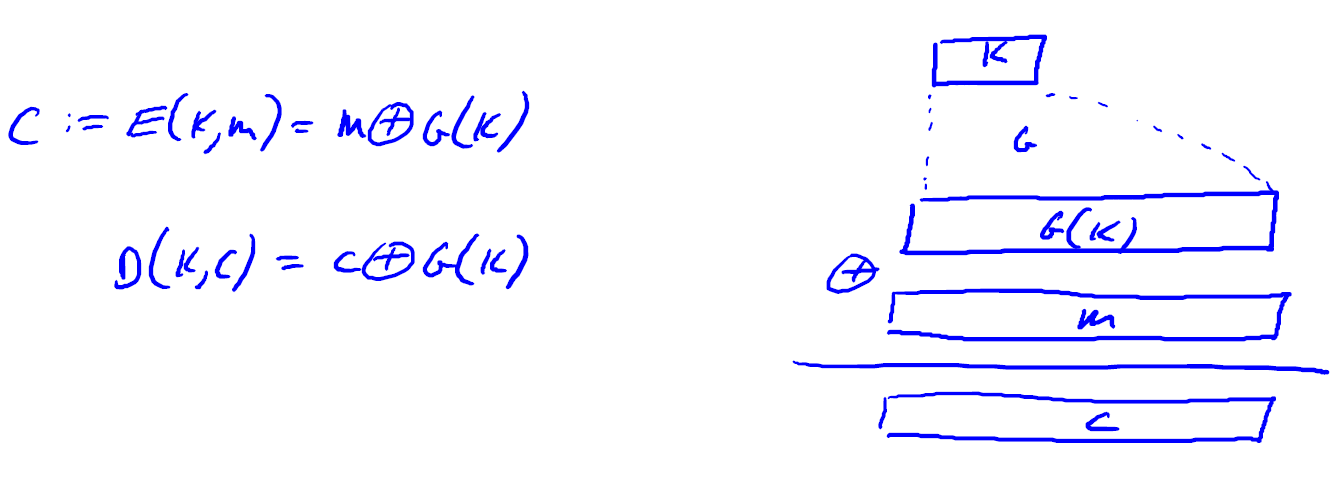
\includegraphics{./Images/PRG.png} Note: PRG should be efficiently
computable by a deterministic algorithm. The key, from the space G(k),
XORed with mssg is a psuedorandom pad and not a truly random pad.

\textbf{Stream Cipher:} A stream cipher is a symmetric key cipher where
plaintext digits are combined with a pseudorandom cipher digit stream
(keystream). In a stream cipher, each plaintext digit is encrypted one
at a time with the corresponding digit of the keystream, to give a digit
of the ciphertext stream. Since encryption of each digit is dependent on
the current state of the cipher, it is also known as state cipher. In
practice, a digit is typically a bit and the combining operation an
exclusive-or (XOR). Note: Stream ciphers convert one symbol of plaintext
directly into a symbol of ciphertext.

\textbf{Redefining Security:} \textbf{Stream ciphers cannot have perfect
secrecy!!} Therefore, we need to rethink how we define security as
perfect secrecy is not practically feasible. So: - Need a different
definition of security - Security will depend on specific PRG
\textgreater{}\textgreater{} Section \ref{prg-security-definition}

\textbf{Fundamental Requirement to secure Stream Ciphers:} A minimal
property that a psuedo random generator must have is property of being
unpredictable, i.e., \textbf{PRG must be unpredictable}. Therefore, for
a stream cipher to be secure, at it's minimum, the PRG it uses must be
unpredictable in nature.

What it mean to be unpredictable for a generator is that given first few
bits of the output of the generator (which is the psuedorandom key), say
1\ldots{}i bits, there is no efficient algorithm that can compute the
rest, i+1\ldots{}n, bits of the stream.

\textbf{Attacks on One Time Pad/Stream ciphers:} - Attack 1: \textbf{Two
time pad is insecure}, i.e., if we used the same key (or psuedorandom
key) to pad two different messages(m1 and m2) and produce c1 and c2
cipher texts then for an adversary who captured both of those cipher
texts, it's fairly easy to recover both m1 and m2 using the CT only
attack. Hence a Stream Cipher key or a One Time Pad key should never,
never ever, be used more than once.
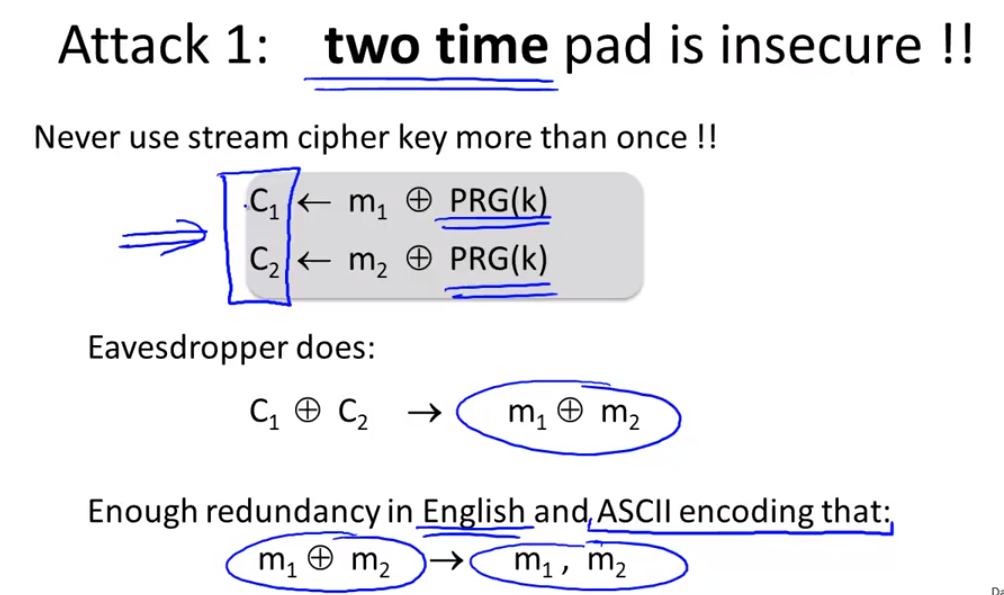
\includegraphics{./Images/TwoTimePad.png} - Attack 2: One Time Pad or
the Stream Ciphers in general provides \textbf{no integrity} at all (all
they do is try to provide confidentiality when the key is only used
once) and therefore are referred as malleables.
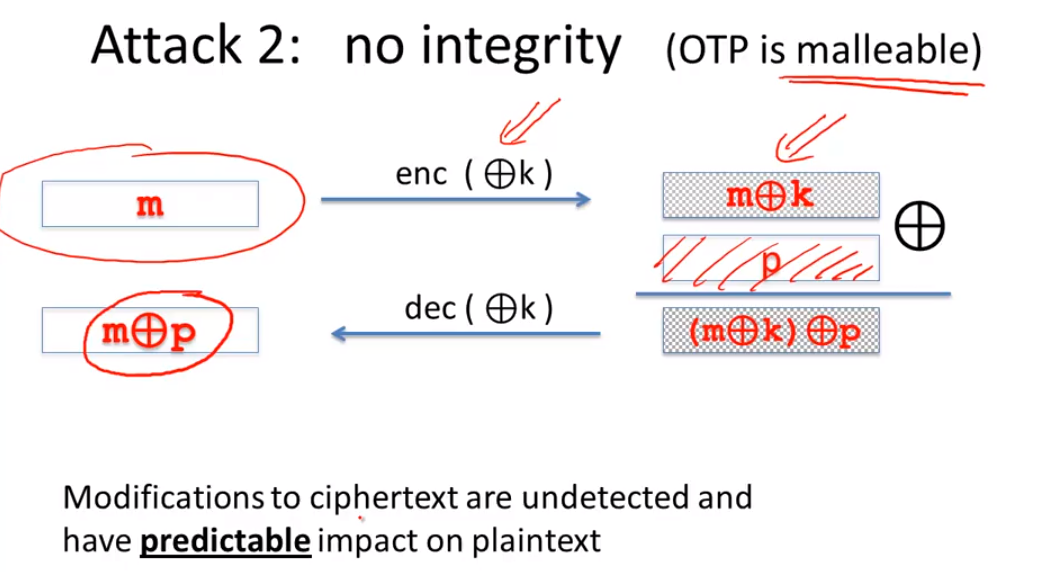
\includegraphics{./Images/MalleableOTP.png}

Real World Examples: - \textbf{Old Stream Ciphers:} RC4, CSS etc. -
\textbf{Modern Stream Ciphers:} eStream project (qualify 5 Stream
ciphers), Modern stream cipher in addition to seed uses nonce which is a
non-repeating value for a given key. Hence, we can reuse a key because
the nonce make the (k, r) pair unique.
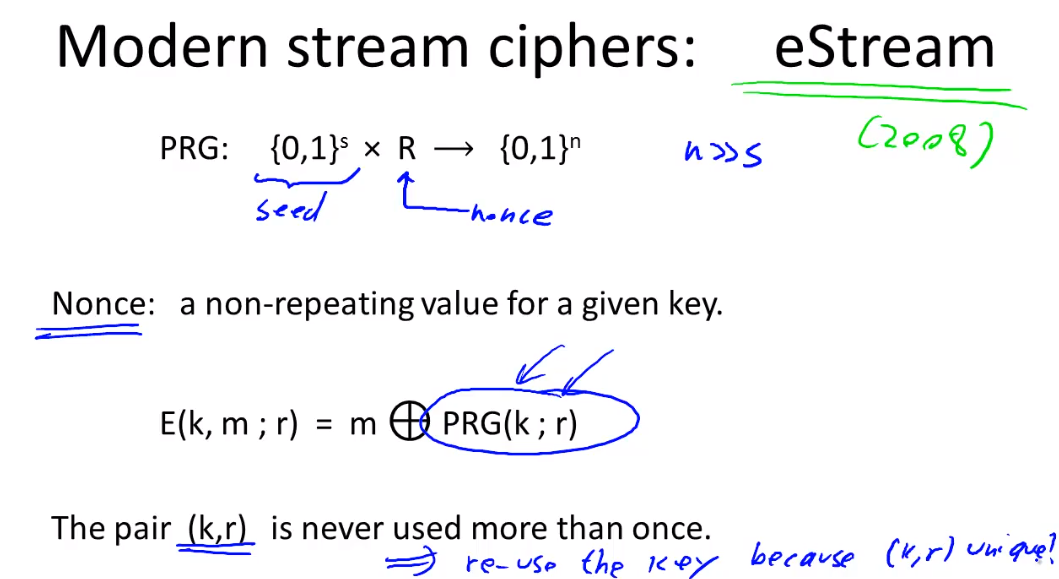
\includegraphics{./Images/ModernStreamCiphers.png}

\begin{center}\rule{0.5\linewidth}{\linethickness}\end{center}

\hypertarget{prg-security-definition}{%
\subsubsection{PRG Security Definition}\label{prg-security-definition}}

Recommended Watch:
\href{https://www.coursera.org/learn/crypto/lecture/De10M/prg-security-definitions}{PRG
Security}

Security of a Stream Cipher depends on how secure is the Psuedo Random
Generator it uses is. In turn the the PRG is regarded as secure if the
output of the PRG is \textbf{indistinguishable from the truly random
output.} That is, the distribution of pseudo random is indistinguishable
from a truly (random) uniform distribution.

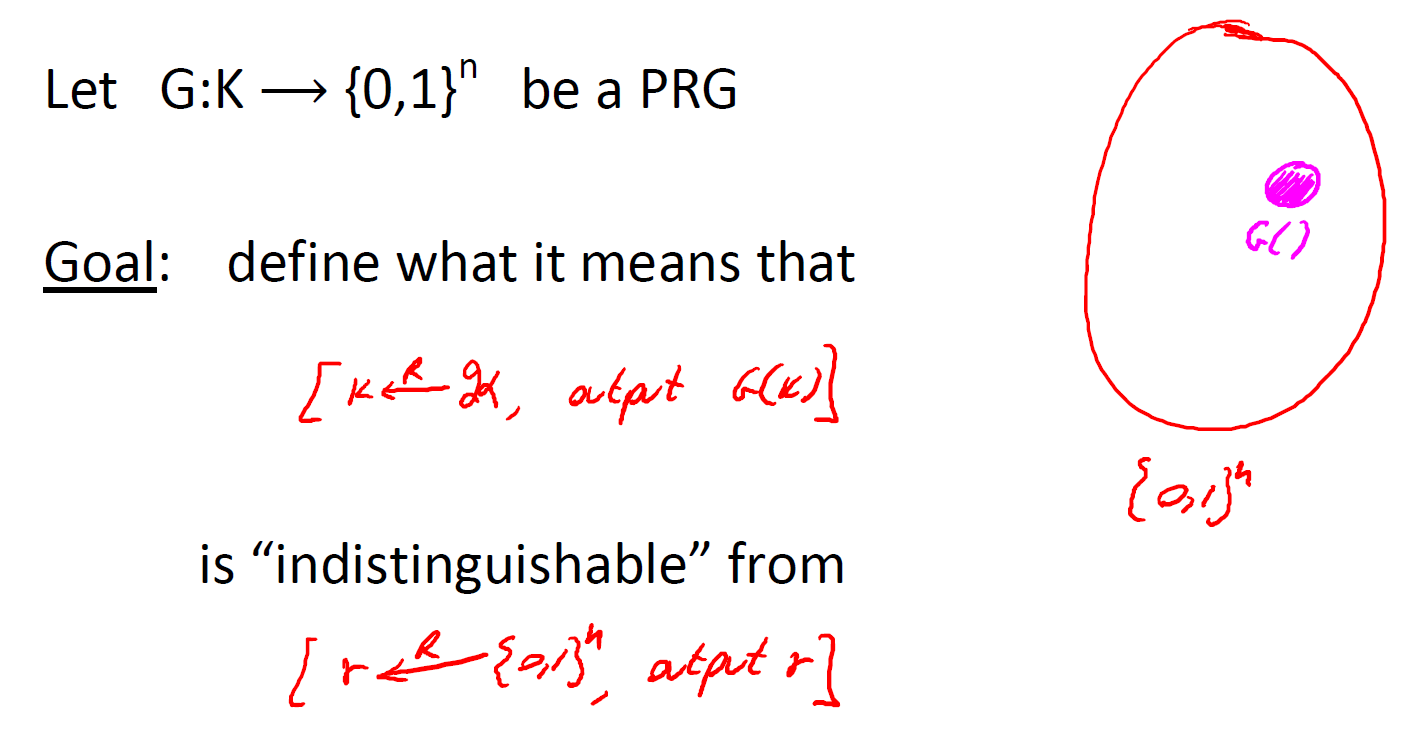
\includegraphics{./Images/IndistinguishablePRG.png} \textgreater{}Goal:
To show that the psuedorandom output G(k), where k is a random variable
from (seed)K = \{0, 1\}\(^{s}\) and G(k) is the psuedorandom output from
the expanded space, \{0 , 1\}\(^n\), of the seed is indistinguishable
from truly random r selected from a key space of \{0, 1\}\(^n\) (not an
expansion space).

How to show this indistinguishability from random? : Using
\textbf{Statistical Test}

\textbf{Statistical Test:} Let's define what is a Statistical test on
space \{0, 1\}\(^{n}\): It's basically an algorithm (A) such that: - A
takes and input x (which is an n bit string) and - Outputs 0 (means
input don't seem random) and 1 (means the input seems to be random)

One can think of any number of statistical tests, therefore, while
considering indistinguishability we only account for efficient
statistical tests.

A statistical test uses the concept of Advantage over a PRG to determine
that whether it could distinguish the psuedorandom input from a truly
random or not. Following image shows the formulation for calculation of
Advantage of a given Statistical test A over a generator PRG.
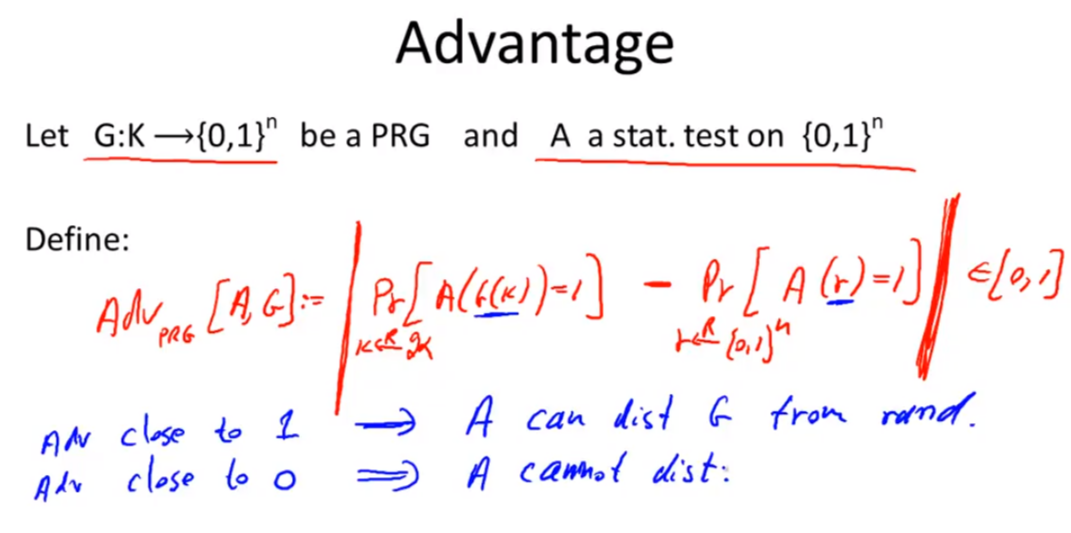
\includegraphics{./Images/Advantage-ST.png} Note: We only want to
consider the advantage of efficient statistical test for the generator
PRG (we don't give a damn about inefficient ones). Also, we want the
advantage to be negligible, i.e., a close to zero as possible (which
indicates the statistical test wasn't able to distinguish).

Hence, crypto definition for a secure PRG is as follows:
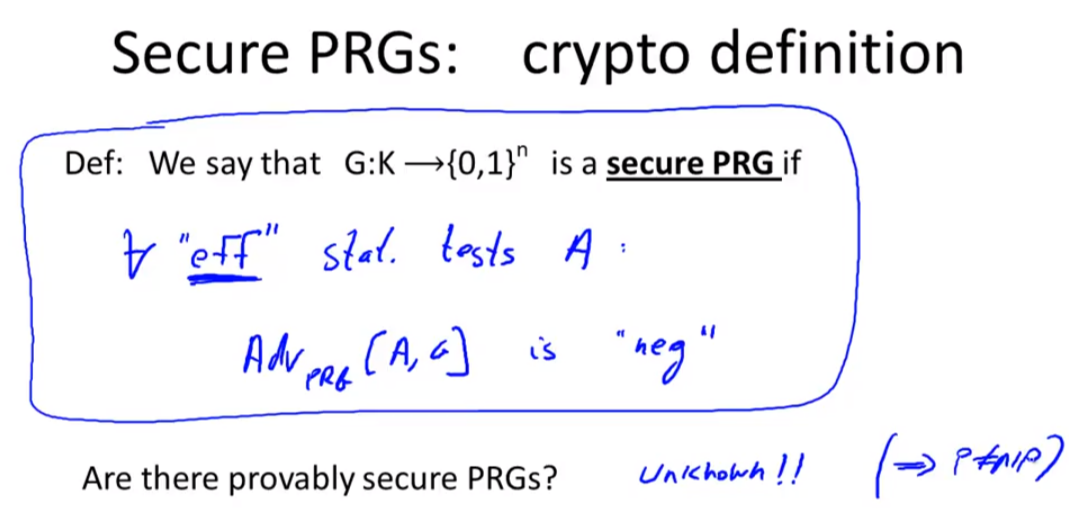
\includegraphics{./Images/SecurePRGs.png} Note: Efficient algo
(statistical test) theoretical means that finishes in polynomial time
and practically could be regarded as one which finishes in a given time.

\textbf{Secure PRG is an unpredictable generator and vice versa}

A secure PRG implies: It's unpredictable (which covers the minimal
requirement for a secure PRG).
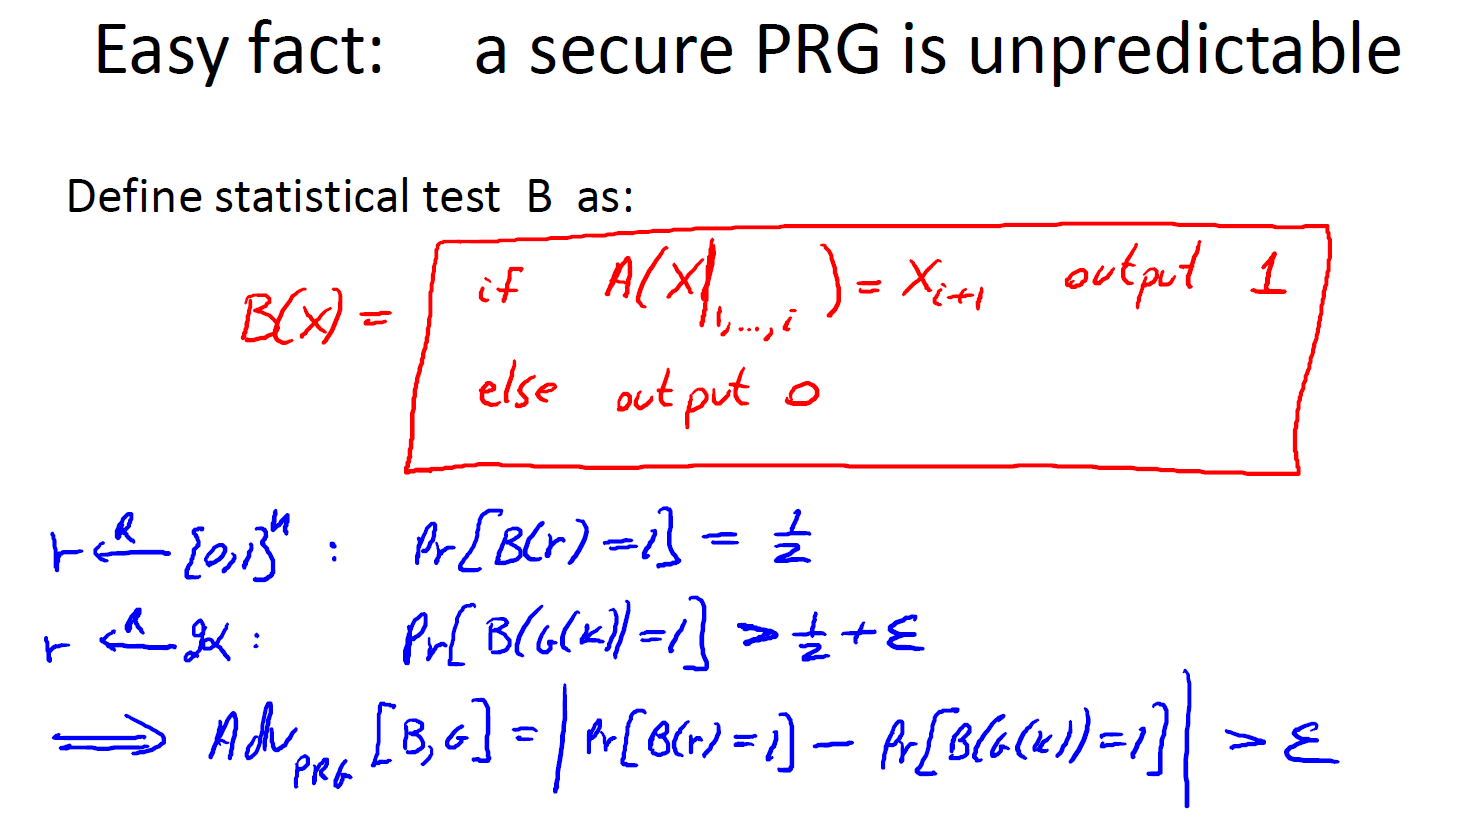
\includegraphics{./Images/SecureMeanUnpredict.png}

Also, there exist a theorem that proved that: an unpredictable generator
is secure in nature. 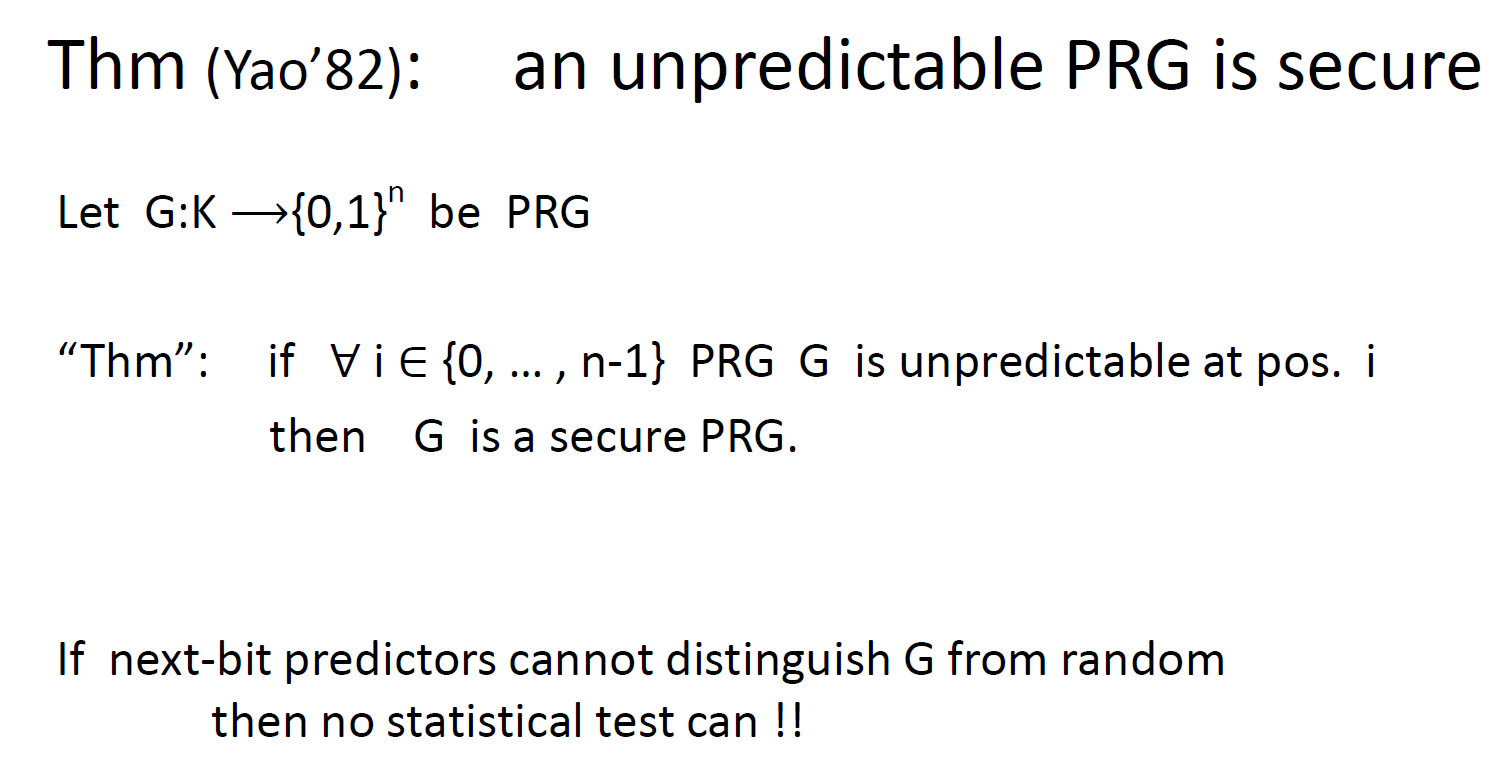
\includegraphics{./Images/UnpredictMeanSecure.png}

\textbf{General Representation:}
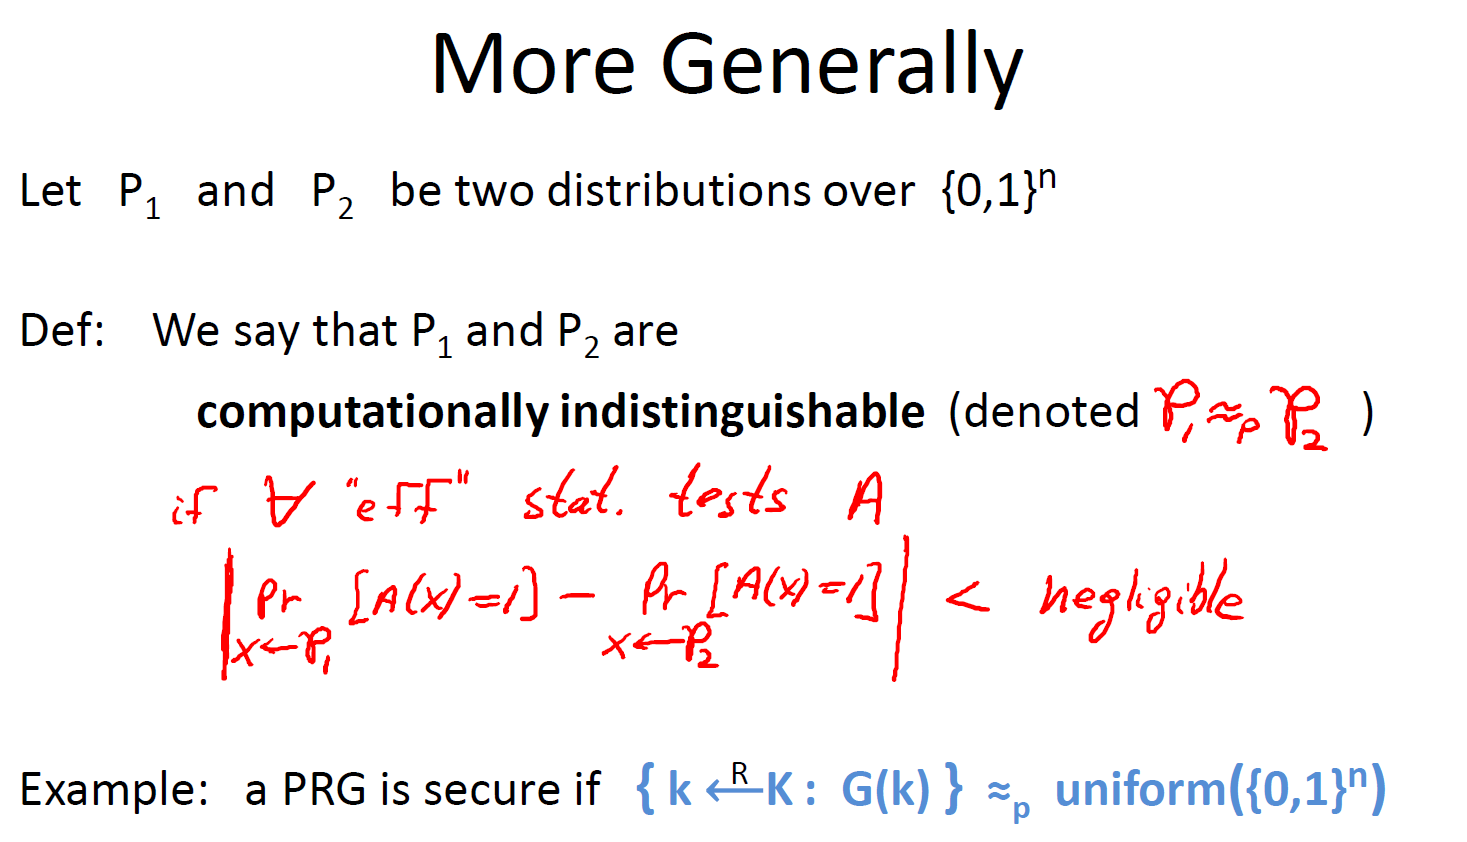
\includegraphics{./Images/GeneralSecure.png} Note: For Stream Cipher,
\(P_{1}\) is G(K) {[}psuedorandom distribution{]} and \(P_{2}\) is a
truly random distribution

\begin{center}\rule{0.5\linewidth}{\linethickness}\end{center}

    \hypertarget{semantic-security}{%
\subsubsection{Semantic Security}\label{semantic-security}}

Recall: Shannon's idea of security: CT should not reveal anything about
PT, this is the concept of semantic security. In semantic security, an
adversary sends 2 messages (of equal length) and our cipher(E) encrypt
it and sends the ciphertext back to the the adversary and if the
adversary have no idea about which message this ciphertext correspond to
then our cipher is said to be semantically secure.

Overview: \textgreater{}An adversary (A) chooses two messages:
\(m_{0}\),\(m_{1}\) and supplies it to the encryption algorithm (E) and
it encrypts one of these messages: c←E(k,\(m_{b}\)) where b = 0, 1 and
offer it back to the adversary. The adversary tries to guess which
message was ciphered and outputs \(b^{'}\) = 0 or 1 corresponding to the
message number that the adversary thinks the ciphertext is encryption of
(either \(m_{0}\),\(m_{1}\)).

Corresponding Watch:
\href{https://www.coursera.org/learn/crypto/lecture/q0h9g/semantic-security}{Semantic
Security}\\
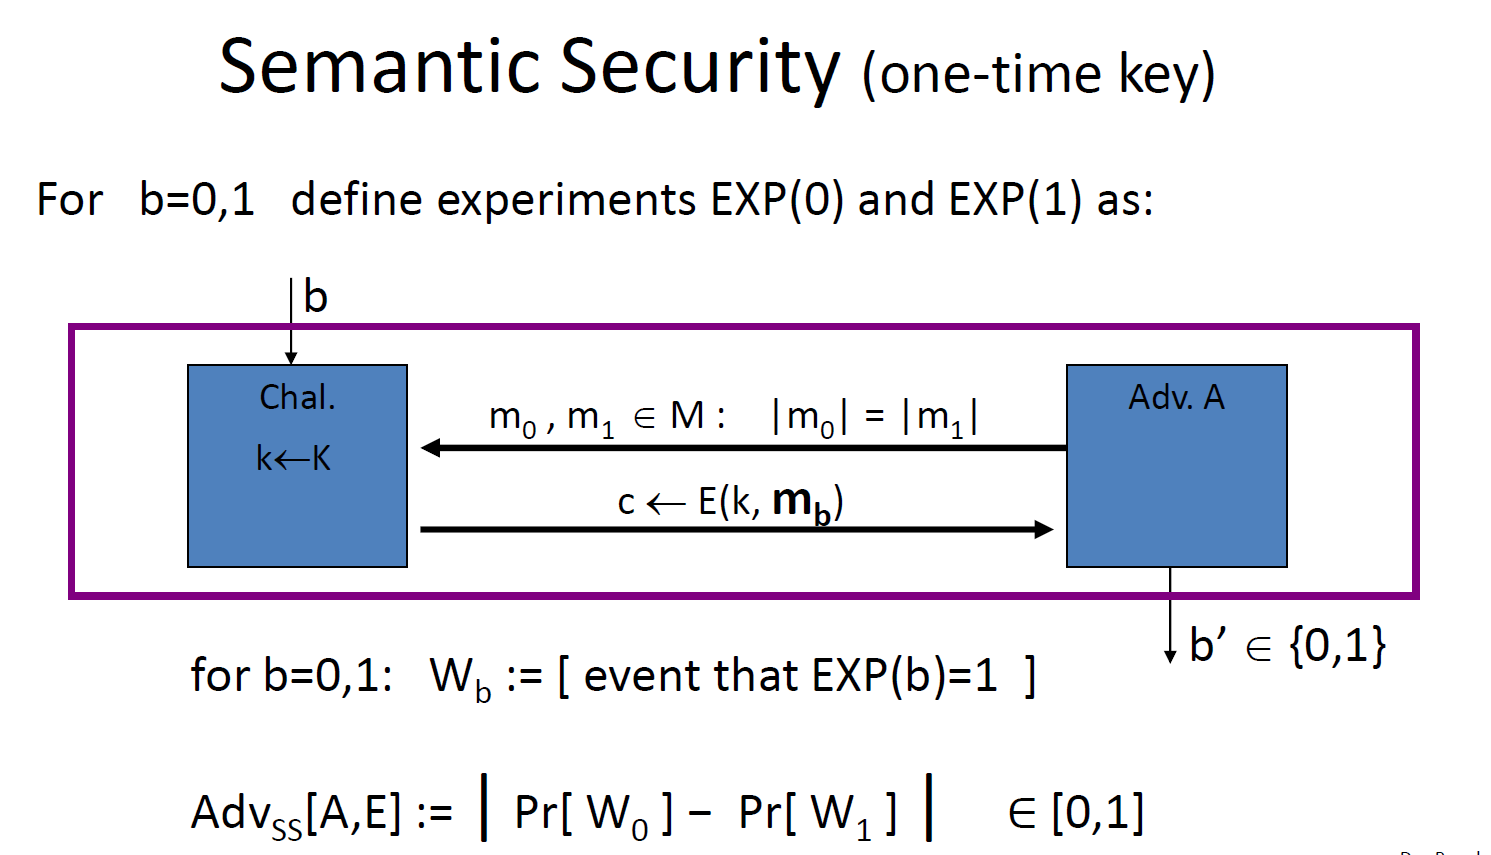
\includegraphics{./Images/SemanticSecurity.png}

Description: \textgreater{}We have 2 experiments, namely Exp(0) and
Exp(1), where in the Exp(0) encryptor (E) gives back the ciphertext for
\(m_{0}\) (out of the supplied two) and in Exp(1) it sends back the
ciphertext for \(m_{1}\). Based on the experiments we have 2 events
\(W_{0}\) and \(W_{1}\) where \(W_{0}\) represents an event where for
Exp(0) adversary outputted \(b^{'}\) as 1 (thinking, wrongly, that the
ciphertext corresponds to \(m_{1}\)). Similarly, \(W_{1}\) represents an
event where for Exp(1) adversary outputted \(b^{'}\) as 1 (rightly
guessed). The advantage is defined such that if the probability of both
the events \(W_{0}\) and \(W_{1}\) is similar or close to each other
then advantage would be close to zero, which would mean that the
adversary isn't able to distinguish that whether the ciphertext was of
\(m_{0}\) or \(m_{1}\).

Note: Semantic Security (One time key) means that the adversary is
provided with only a single ciphertext (which could correspond to any of
the two supplied message).

\textbf{E is said to be semantically secure if for all ``efficient'' A
(adversary), Adv\(_{SS}\) {[}A, E{]} = negligible.}

OTP is semantically secure (it has perfect semantic security due to
uniform probability distribution):
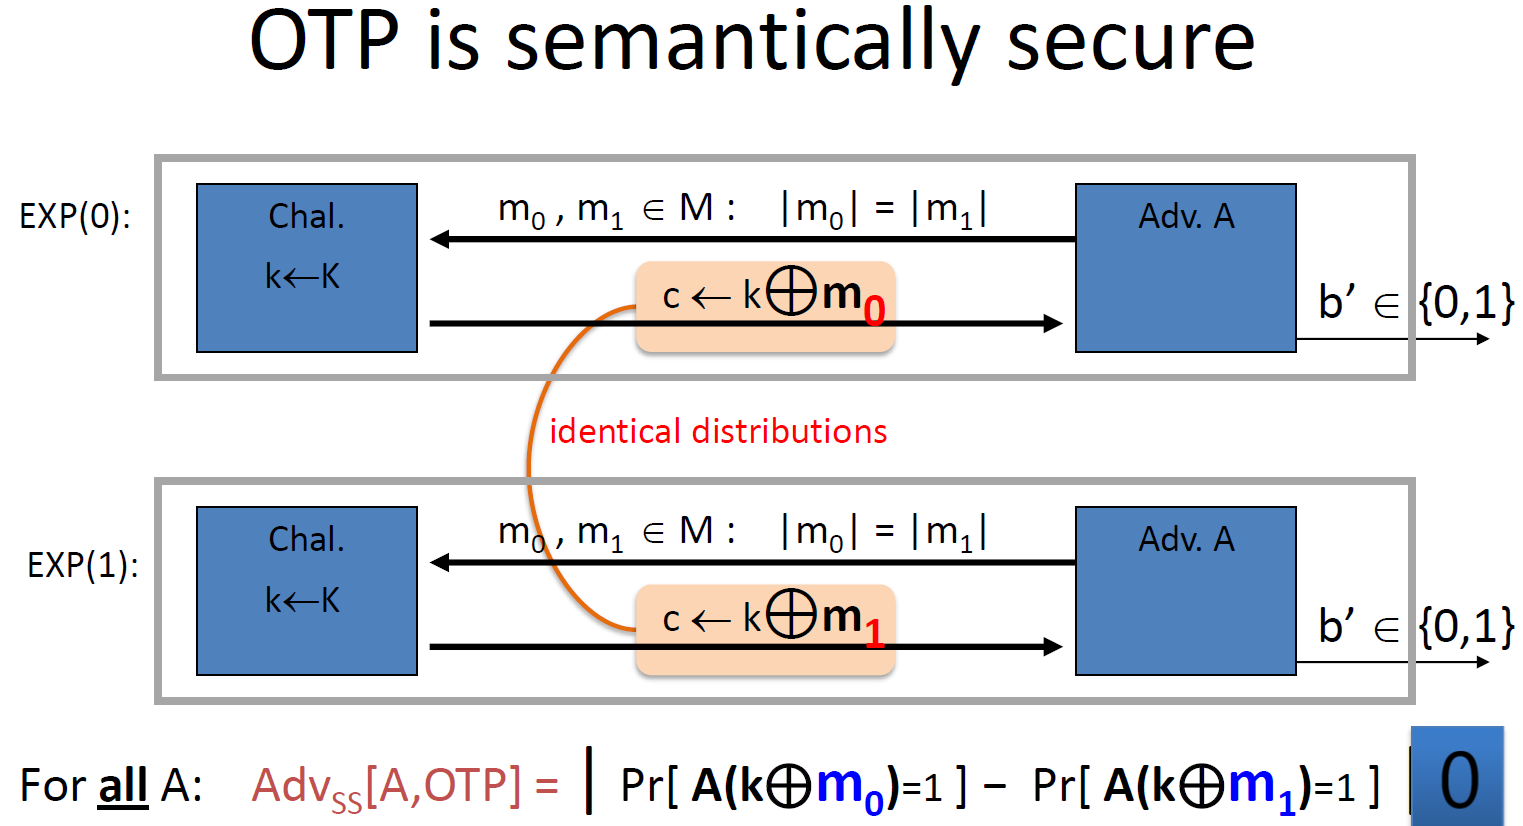
\includegraphics{./Images/OTPSemantic.png}

\begin{quote}
Theorem: \textbf{Given that G is a secure PRG (i.e.~holds the
indistinguishability property). A Stream Cipher E derived from or
incorporates G is semantically secure.}
\href{https://www.coursera.org/learn/crypto/lecture/VeLNT/stream-ciphers-are-semantically-secure-optional}{Proof!!}
\end{quote}

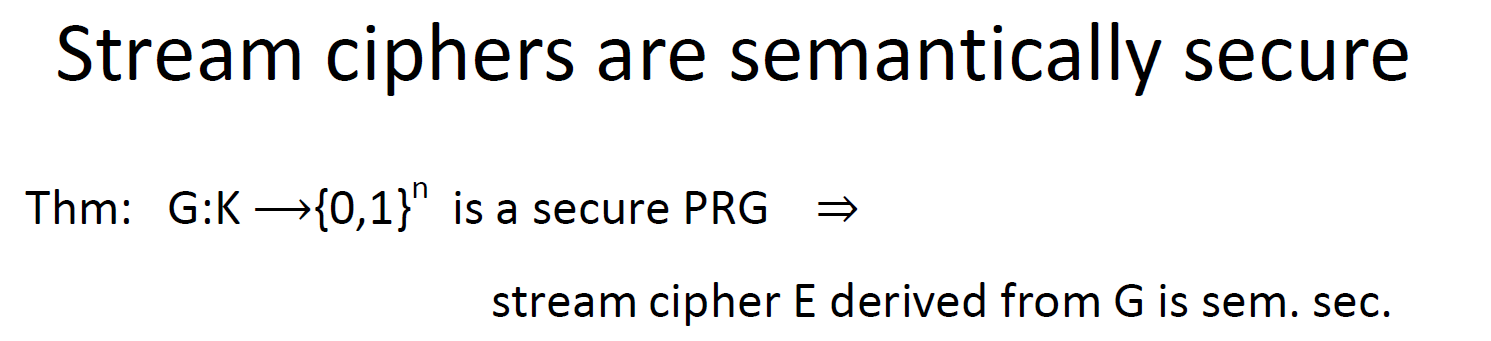
\includegraphics{./Images/StreamSemantic.png}

\begin{center}\rule{0.5\linewidth}{\linethickness}\end{center}

    \hypertarget{block-ciphers}{%
\subsubsection{Block Ciphers}\label{block-ciphers}}

Overview: \textgreater{}A block cipher is an encryption method that
applies a \textbf{deterministic algorithm along with a symmetric key to
encrypt a block of text}, rather than encrypting one bit at a time as in
stream ciphers. For example, a common block cipher, AES, encrypts 128
bit blocks with a key of predetermined length: 128, 192, or 256 bits.
\textbf{Block ciphers are pseudorandom permutation (PRP) families} that
operate on the fixed size block of bits. Note: PRPs are functions that
cannot be differentiated from completely random permutations and thus,
are considered reliable, until proven unreliable.

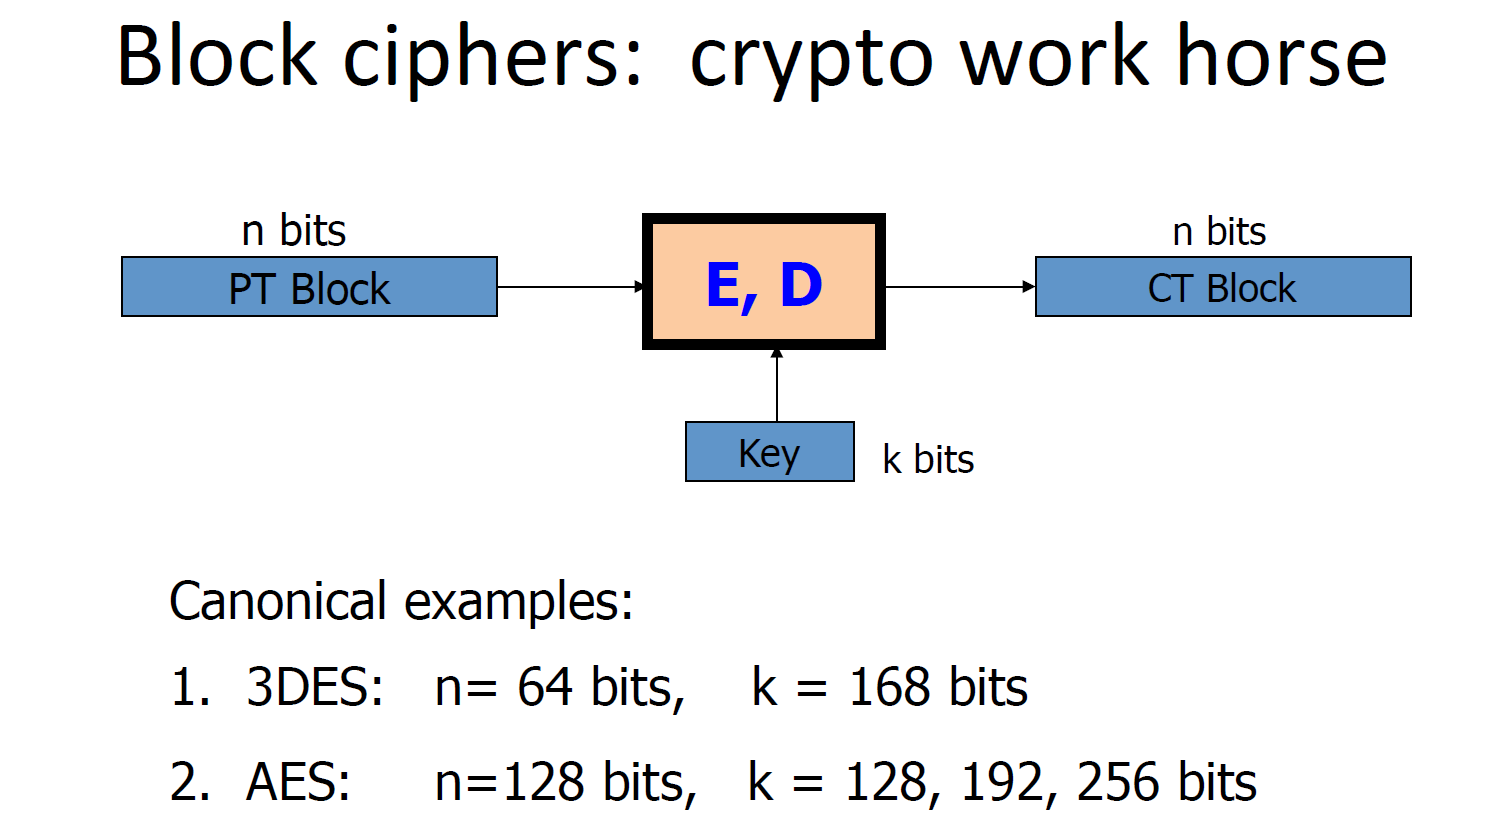
\includegraphics{./Images/BlockCiphers.png}

Block cipher \textbf{modes of operation have been developed to eliminate
the chance of encrypting identical blocks of text the same way}, the
ciphertext formed from the previous encrypted block is applied to the
next block. A block of bits called an \textbf{initialization vector
(IV)} is also used by modes of operation to ensure ciphertexts remain
distinct even when the same plaintext message is encrypted a number of
times.

Some of the various modes of operation for block ciphers include
\textbf{CBC} (cipher block chaining), \textbf{CFB} (cipher feedback),
\textbf{CTR} (counter), and \textbf{GCM} (Galois/Counter Mode), among
others. Above is an example of CBC mode. Where an IV is crossed with the
initial plaintext block and the encryption algorithm is completed with a
given key and the ciphertext is then outputted. This resultant cipher
text is then used in place of the IV in subsequent plaintext blocks.

\textbf{Working of Block Ciphers (Generic):}

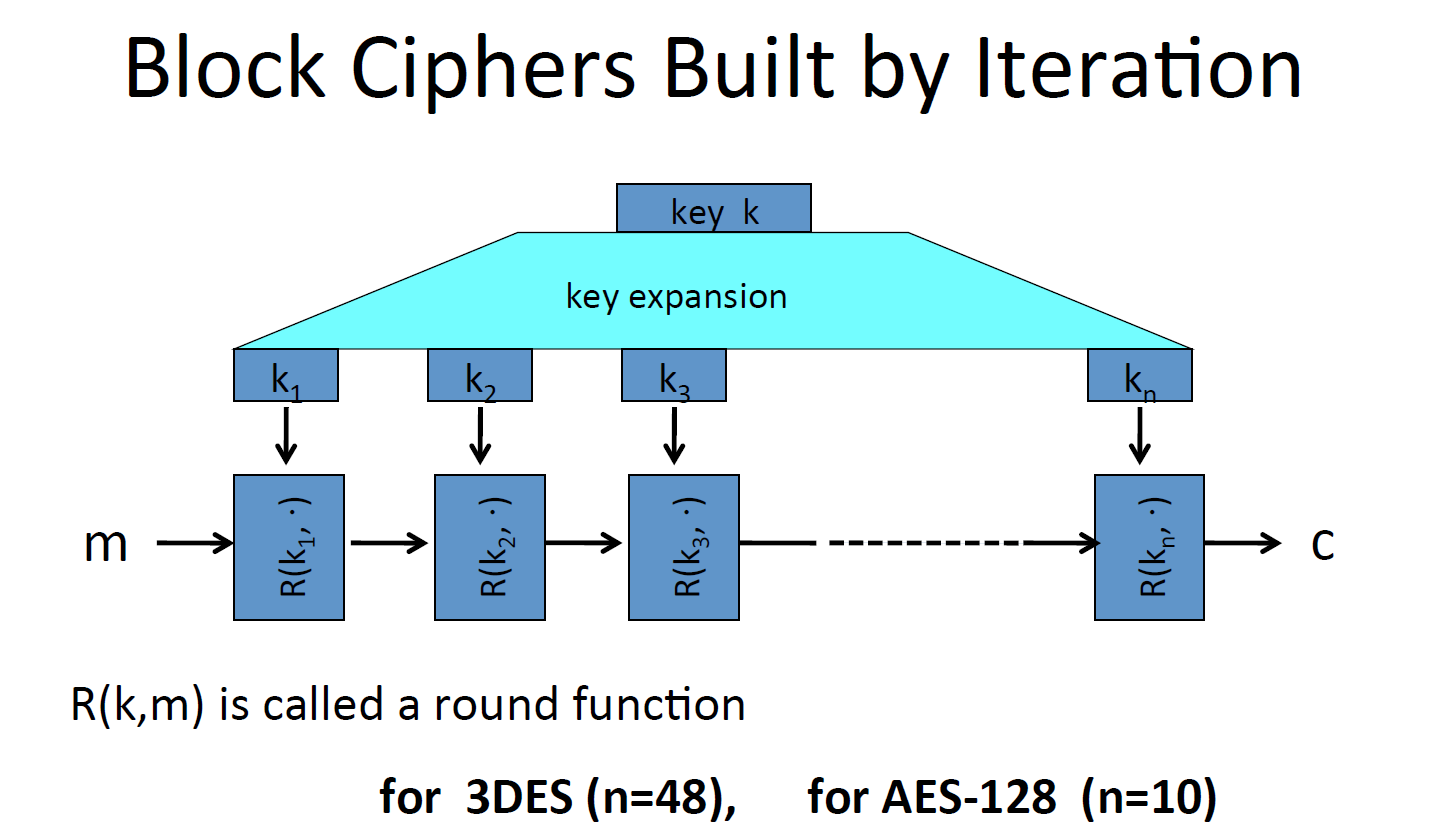
\includegraphics{./Images/BlockCipher-Working.png} Description: 1. key
is expanded into n number of keys called round keys (where n is the
number of rounds which is subjective to individual block cipher). 2.
Cipher uses these round keys by iteratively encrypting the message again
and again and again using what's referred to as the round function. 3.
Round function takes 2 inputs: Current state of the message and a round
key (corresponding to that round). 4. The output of one round function
acts as the new state of the original message which is fed into the next
round function. The output from the \(n^{th}\) round function is the
ciphertext.

In order to specify a particular block cipher (built by iteration, like
DES) one has to specify the key expansion mechanism and the round
function. (Those are the two dynamic part of a block cipher).

Note: Block ciphers are relatively slower than the stream cipher (and
slower by large magnitude to eStream ciphers) but we will see that we
can do many things with block ciphers that we couldn't do very
efficiently with stream ciphers.

\textbf{Block Cipher aka Psuedo Random Permutation (PRP)} PRP accurately
captures what a block ciphers basically is, in other words, \textbf{PRP
is a mathematical abstraction of a Block Cipher}. How? \textgreater{}As
per my perception: A block cipher with size of the key as K, used (to
say XOR), dictates the size of the block of the message M. Hence
limiting the size of message block from its true gigantic universe to a
small key-size universe and while we operate the key onto the message
block the resultant/output is another state of the message belonging
from the key-size universe (i.e.~with the help of key we mapped the
current state of message from the key-sized message universe to another
state in itself, in a one-to-one mapping fashion, therefore permuted).

Therefore, in many places PRPs and block ciphers are used interchangebly
depending on the context.

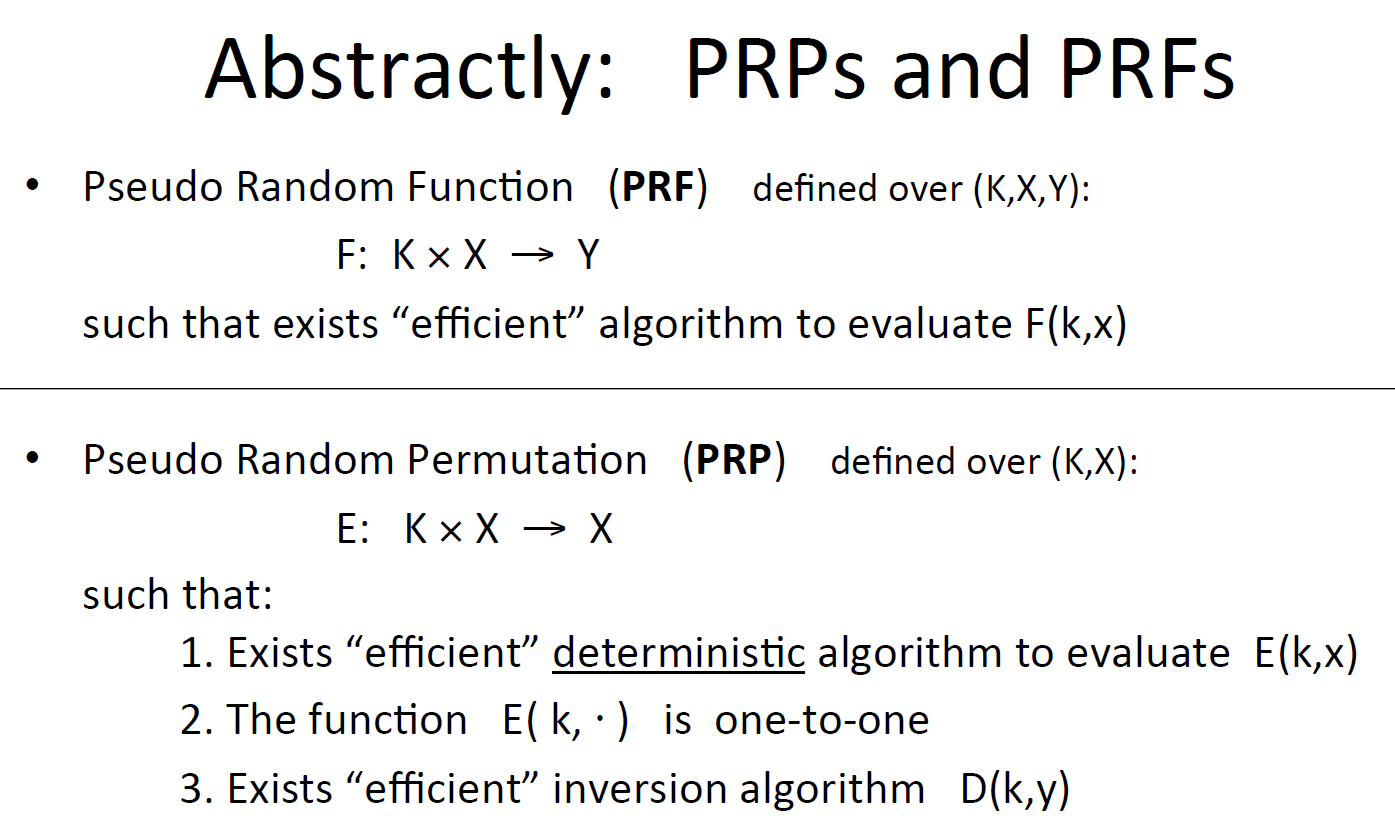
\includegraphics{./Images/PRP.png} where, - PRF: {[}K: Key, X: Input
domain, Y: Output domain{]} - PRP: {[}K: Key, X: Input and Output
Domain{]}

\textbf{Why Block ciphers are PRPs and not PRFs?} \textgreater{} Because
PRF may or maynot be invertible, however, PRPs are by definition
invertible (with one-to-one mapping) and block ciphers needs to be
invertible for being able to be decrypted using the reverse process of
the encryption mechanism (as we will see in DES, AES etc.), and
therefore PRPs capture the essence of block ciphers.

Explanatory Read:
\href{http://www.crypto-it.net/eng/theory/prf-and-prp.html}{Psuedorandom
Functions and Permutations}

\includegraphics{./Images/PRP\&PRF.png}

\begin{center}\rule{0.5\linewidth}{\linethickness}\end{center}

    \hypertarget{secure-block-cipher}{%
\paragraph{Secure Block Cipher:}\label{secure-block-cipher}}

Explanatory video:
\href{https://www.coursera.org/learn/crypto/lecture/t4JJr/what-are-block-ciphers}{Block
Ciphers and Secure PRFs}

Exploring what it means for a PRP or PRF (in general) to be secure and
this concept will essentially captures what it means for a block cipher
to be secure.

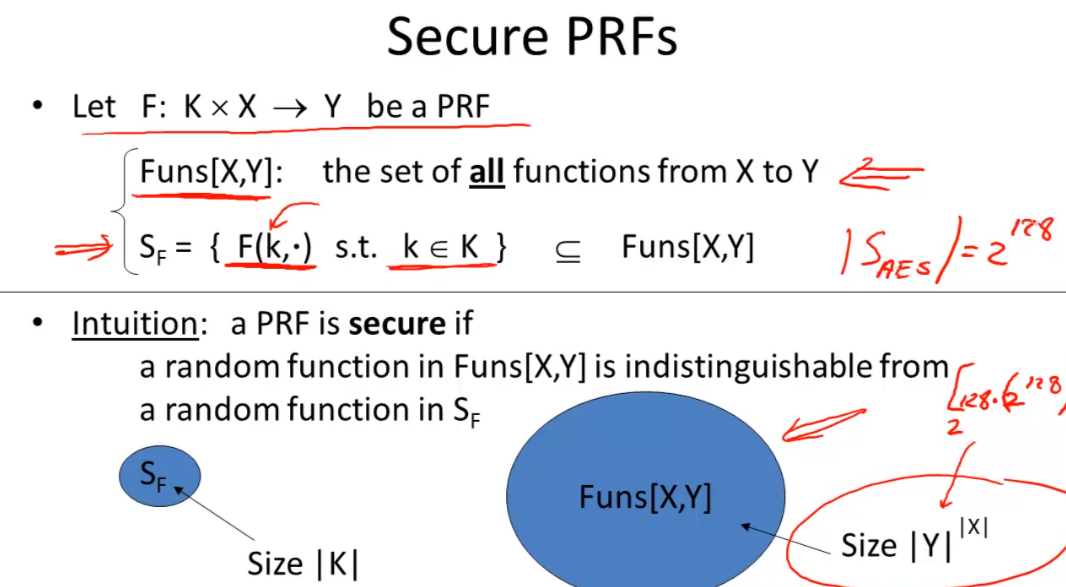
\includegraphics{./Images/SecurePRF.png} Description: - The set of all
the possible function from X to Y is gigantic which is referred, above,
as Funs{[}X,Y{]}. However, we get a relatively smaller set of functions
\(S_{F}\) (which is regarded as a set of psuedo random function cuz it
is in some sense determined by the key) when we restrict the size of X
to be equal to the size of key (as we have to perform XOR or another
operation b/w input domain X and Key K, therefore there lengths must be
equal). - Hence, the PRF is restricted in it's domain by the size of the
key (say 128 bits for AES then domain is of size \(2^{128}\)). - Given
that \(S_{F}\) \textless{}\textless{}\textless{}\textless{} Funs{[}X,
Y{]} a PRF is considered secure if the uniform distribution from a set
of psuedo random functions (\(S_{F}\)) is indistinguishable from the
uniform distribution of truly random functions (Funs{[}X,Y{]}).

Note: The above is a description for a secure PRF. For a secure PRP
instead of choosing a random function from X to Y we are going to choose
a random permutation on the set X (Perms{[}X{]}), in other words, a
random one-to-one function on the set x. The adversary can either query
this random permutation on the set X or it can query a psuedo random
permutation \(S_{F}\) (which is \textless{}\textless{}\textless{} then
random permutation Perms{[}X{]}) and if the adversary cannot tell the
difference then the PRP is secure.

\textbf{Secure PRP Implies a Secure PRF}
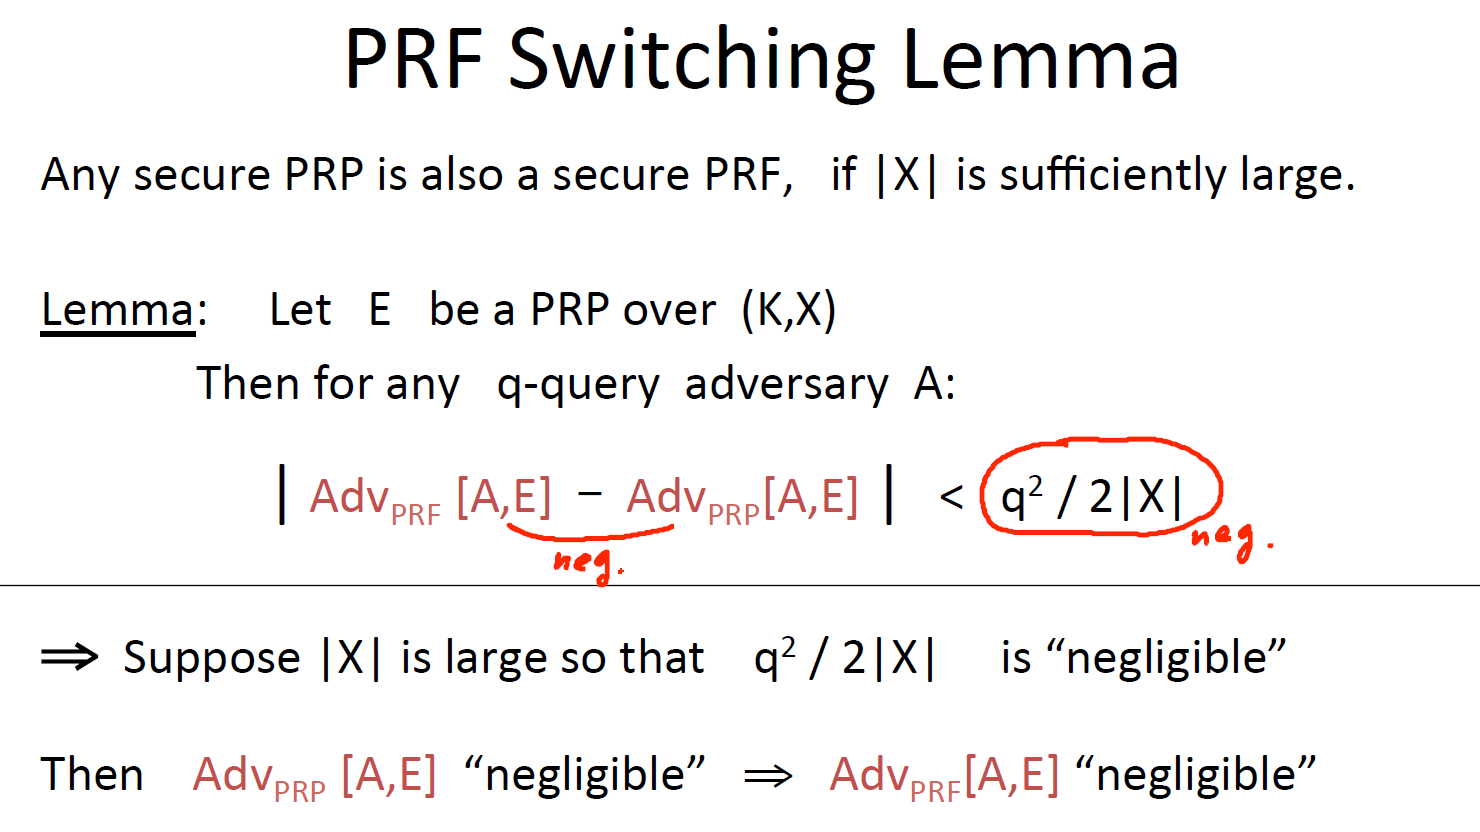
\includegraphics{./Images/SecurePRP2PRF.png}

\textbf{Relation between PRF(Psuedo Random Functions) and PRG (Psuedo
Random Generators):} 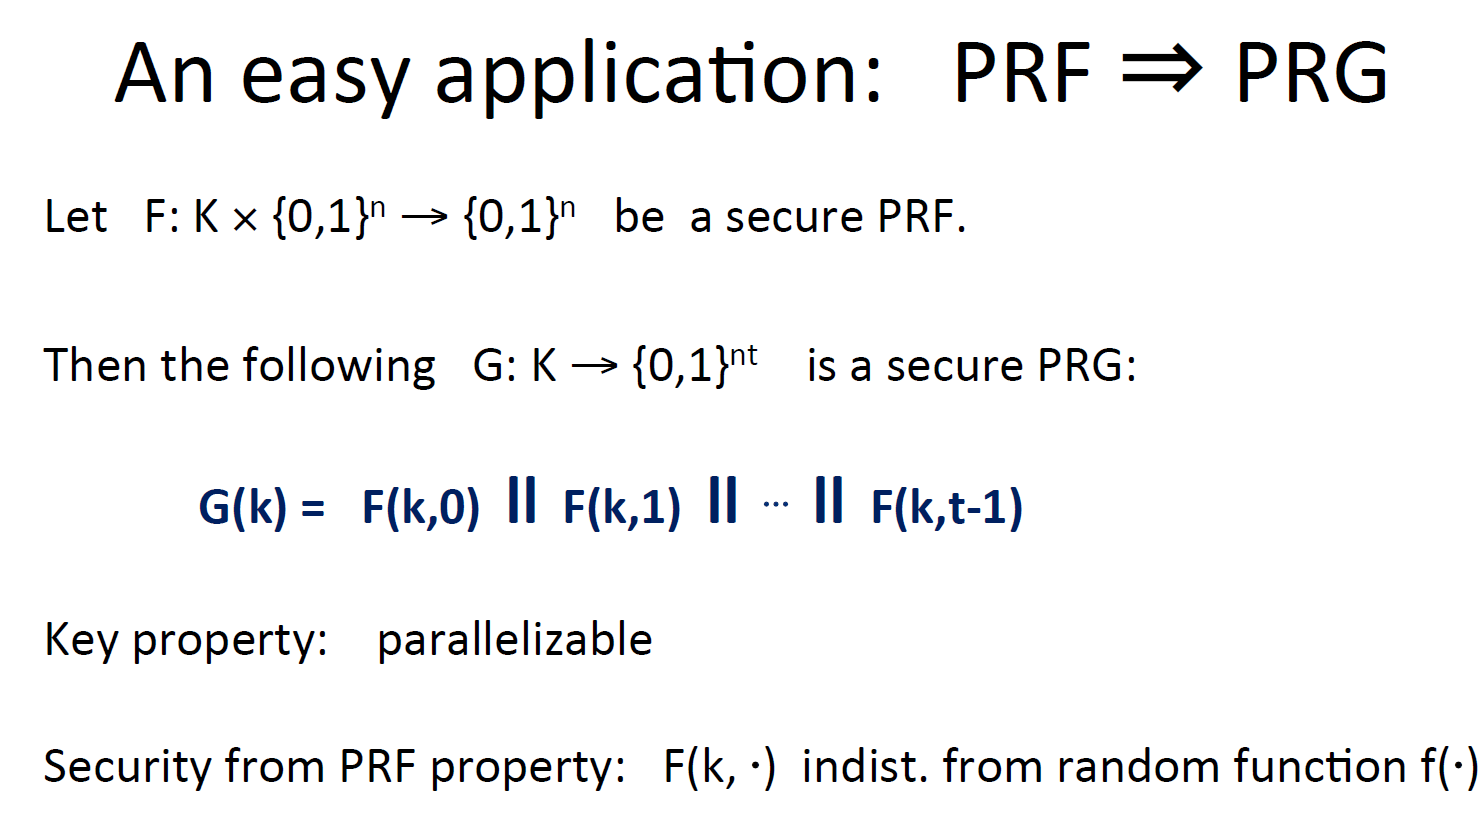
\includegraphics{./Images/PRF2PRG.png} Description:
- Assume we have a psuedo random function F (here, it's PGP as defined
one to one on \{0, 1\}\(^{n}\)) which is secure. - Now we define a PRG
(G) whose seed space (K) is same as the Key Space (K) for the PRF and
its output space is basically going to be t blocks of n bits each and
concatenated to get the generator value. So we basically took the key of
the PRF and expanded to t times of n bits each. - Key property of such a
generator would be that it's parallelizable, which means, if we have 2
cores to compute on than we can compute the even entries on one core and
odd entries on the other and concatinate at the end. Hence, we a cipher
using such a generator would be paralellizable. Where as many of the
previous stream ciphers that we looked before were inherently sequential
like RC4 which therefore can't take the advantage of multi cores. - Such
a PGF derived PGR is secure because the PGF is indistinguishable from
truly random therefore as we can see the Generator is just a
concatination of t different PGFs and hence it would also be
indistinguishable and therefore secure in nature.

Bottom line: A secure PRF gives rise to secure PRG which has this key
property of being parallelizable.

\begin{center}\rule{0.5\linewidth}{\linethickness}\end{center}

    \hypertarget{des-data-encryption-standard}{%
\subsubsection{DES (Data Encryption
Standard):}\label{des-data-encryption-standard}}

Recommended Watch: -
\href{https://www.youtube.com/watch?v=Y61qn_SQl40}{DES Explained
Concisely} -
\href{https://www.coursera.org/learn/crypto/lecture/TzBaf/the-data-encryption-standard}{DES
In Depth}

Read:
\href{https://www.tutorialspoint.com/cryptography/data_encryption_standard.htm}{DES
Quick Read}

The Data Encryption Standard (DES) is a symmetric-key block cipher which
is an implementation of a Feistel Network. It uses 16 round Feistel
structure. The block size is 64-bit. Though, key length is 64-bit, DES
has an effective key length of 56 bits, since 8 of the 64 bits of the
key are not used by the encryption algorithm (function as check bits
only). General Structure of DES is depicted in the following
illustration:

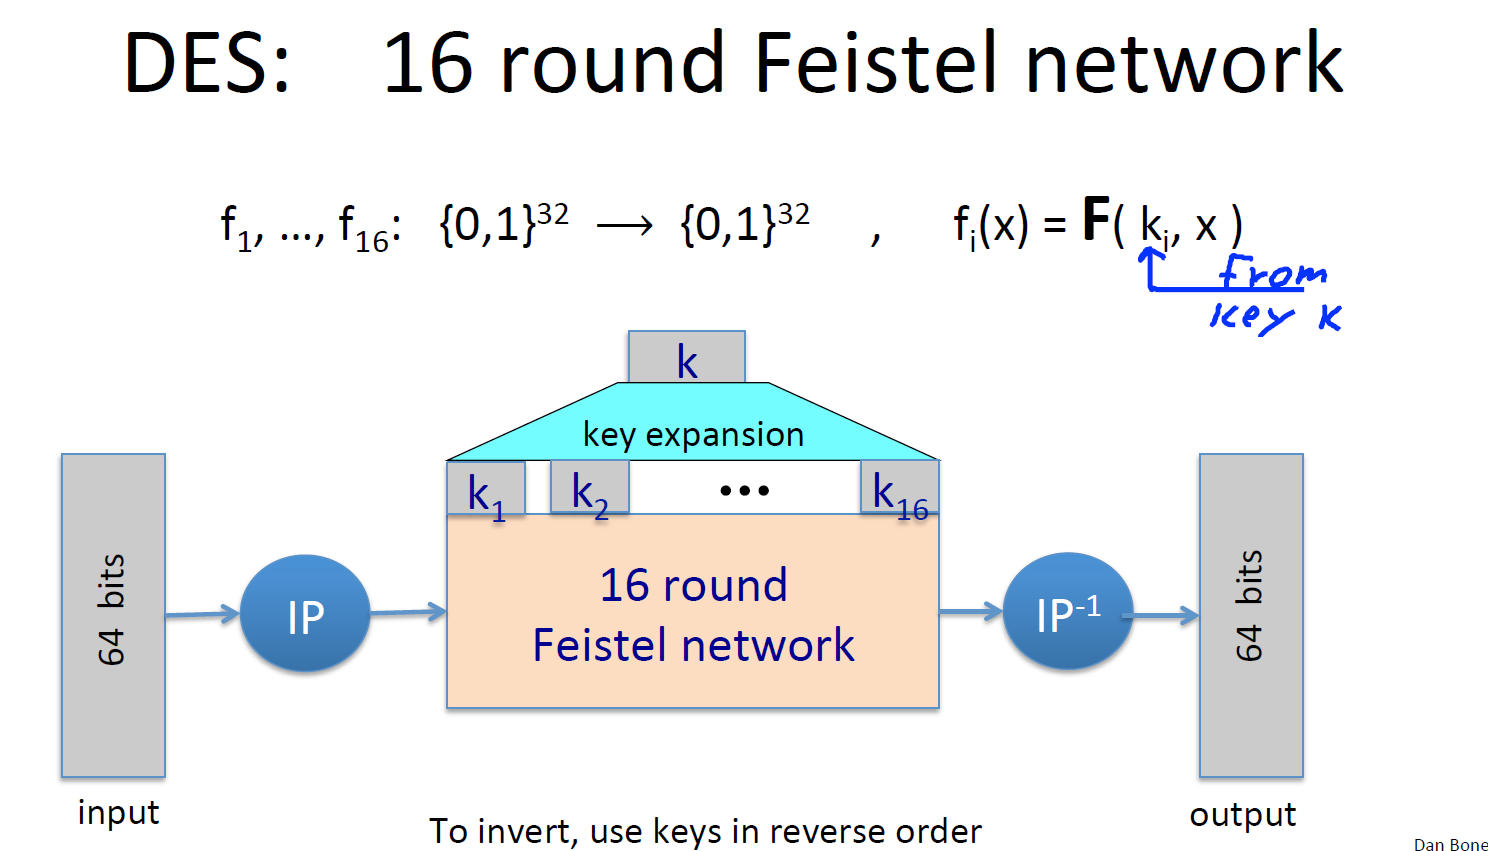
\includegraphics{./Images/DES.png} where, {[}IP: Initial Permutation{]}

\textbf{Fundamental Component of DES: The Feistel Network:}
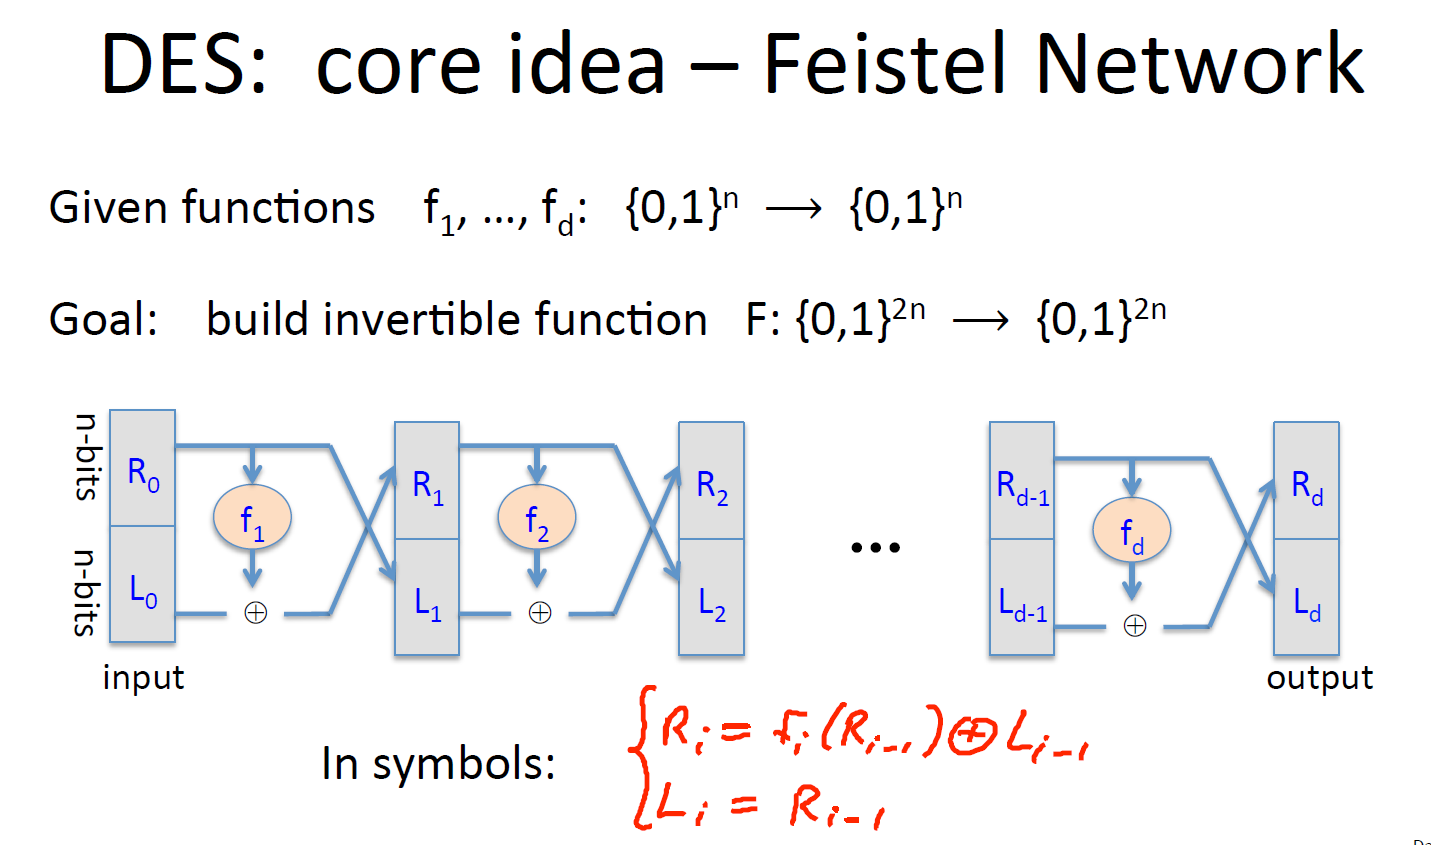
\includegraphics{./Images/FeistelNetwork.png}

The key property of the Feistel Network is that it is invertible:
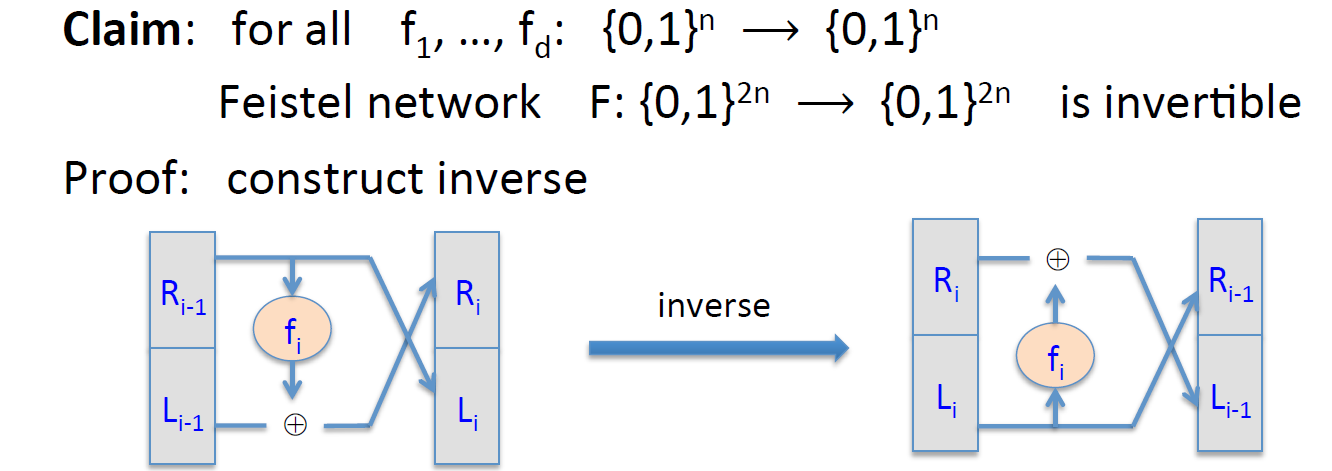
\includegraphics{./Images/Invertible-Feistel.png}

This property of the Feistel Network results in an easy formulation of
the Decryption algorithm for DES.
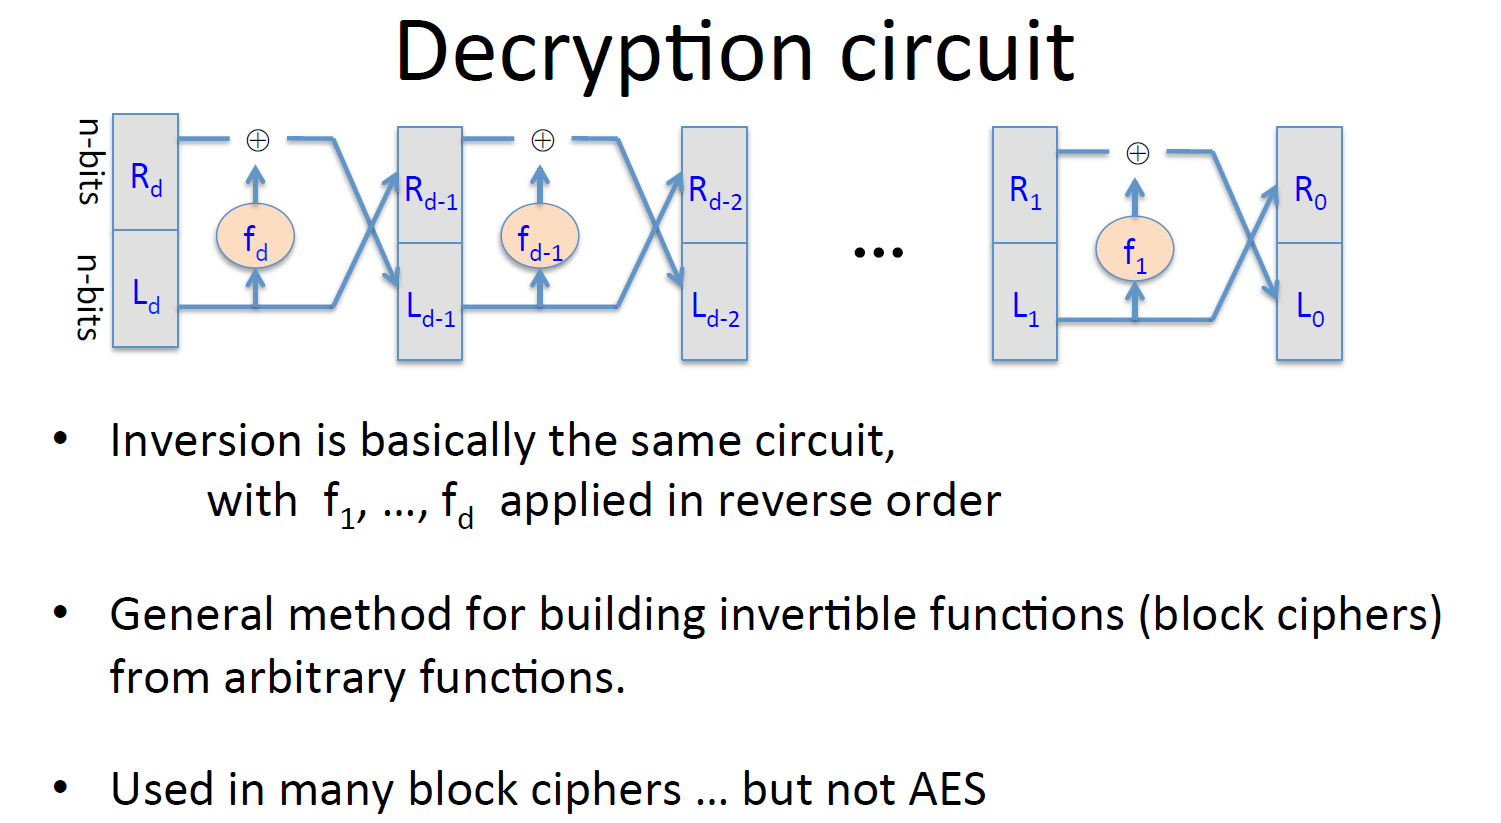
\includegraphics{./Images/DES-Decryption.png} Note: The Feistel
mechanism is a general method for making invertible functions from
arbitrary functions and is infact used in many different block ciphers.
Although, interestingly it's not used in AES.

\textbf{Is DES a secure block cipher?} There is this theorem that
states: given that we use a secure PRF (F) in each round, then a 3-round
Feistel network (therefore, also a 16 round Feistel network i.e.~DES),
with 3 independently derived keys being passed to F, results in a secure
PRP (which implicitly means a secure block cipher).
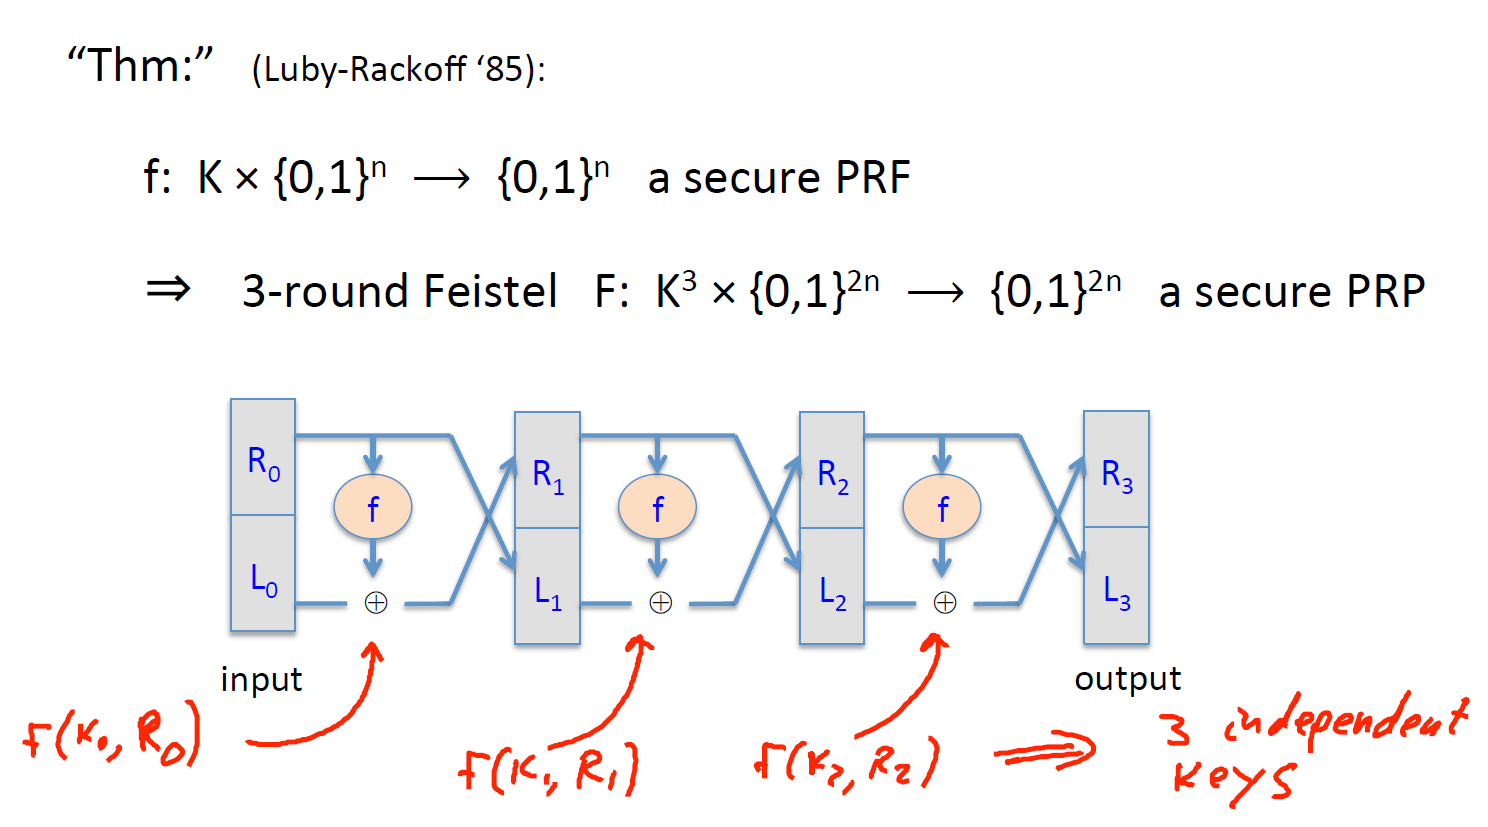
\includegraphics{./Images/SecureFeistel.png}

\textbf{Overview of DES and the Round function:}

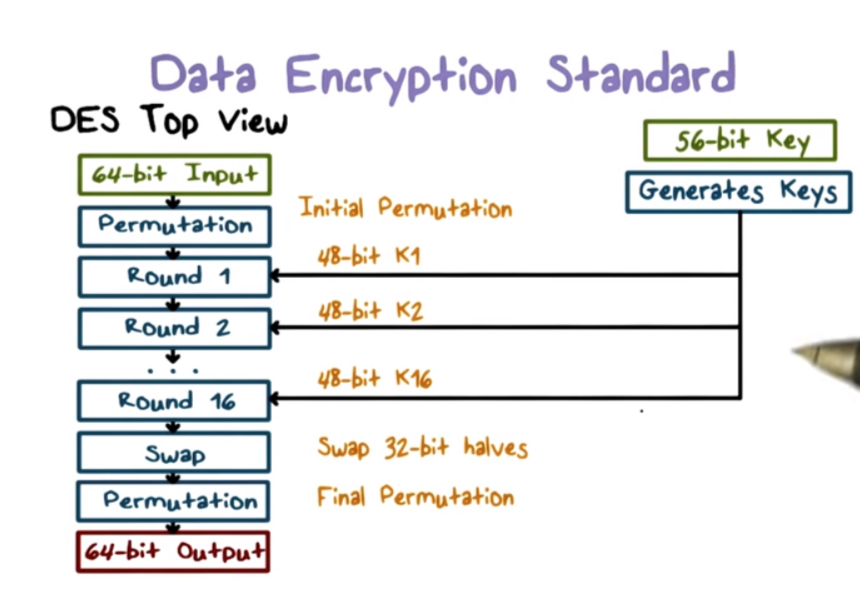
\includegraphics{./Images/DES-View.png}

The heart of DES cipher is the round function. The function applies a
48-bit key to the rightmost 32 bits to produce a 32-bit output.
Following are the steps:

\begin{itemize}
\tightlist
\item
  \textbf{Expansion Permutation Box:} Since right input is 32-bit and
  round key is a 48-bit, we first need to expand right input to 48 bits.
\item
  \textbf{XOR (Whitener):} After the expansion permutation, DES does XOR
  operation on the expanded right section and the round key to generate
  a 48-bit output. The round key is used only in this operation.
\item
  \textbf{Substitution Boxes:} The S-boxes carry out the real mixing
  (confusion). DES uses 8 S-boxes, each with a 6-bit input and a 4-bit
  output. There are a total of eight S-box tables taking a 48-bit input.
  The output of all eight s-boxes is then combined in to 32 bit section.
\item
  \textbf{Straight Permutation:} The 32 bit output of S-boxes is then
  subjected to the straight permutation.
\end{itemize}

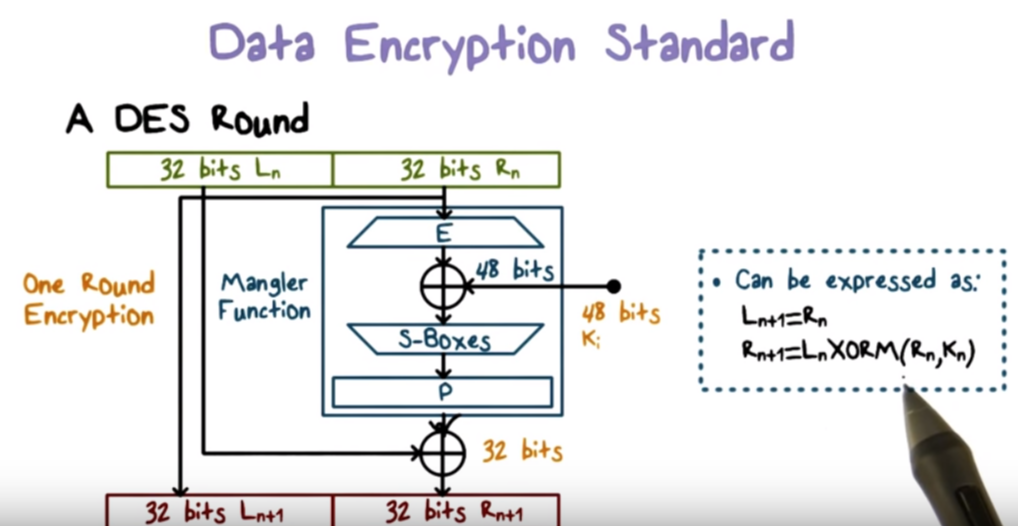
\includegraphics{./Images/DES-Round.png}

\textbf{Status of DES:} DES is no more recommended for use in production
level applications as it can be broke using exhaustive search (brute
force over the entire key space) attacks and now a days with the present
hardware we can recover a DES key within 24 hours, hence highly
insecure. Also, there are many more types of attacks that DES is
subjected to like: linear and differential attacks and quantum
exhaustive attacks. DES has been superseded by the more secure Advanced
Encryption Standard (AES) algorithm. Bottom line: \textbf{DES is
completely DEAD} {[}i.e.~56-bits ciphers shouldn't be used anymore{]}.

As DES was really popular it was deployed at many places and a lot of
hardware support was developed for it, then naturally the next question
was what to do next and organically people thought that in order to
thwart the exhaustive search lets increase the key space such that it
becomes computationally infeasible to do an exhaustive search attack.
Hence, \textbf{Triple-DES} was born.

\textbf{Triple DES:} It has, as the name says, triple the key
space(\(2^{168}\)) of the normal DES, however it is 3 times slower as
well. There is still an attack that can be done on 3-DES in \(2^{118}\),
but practically it takes too long to perform. In general, anything that
has a key space beyond \(2^{90}\) is considered secure to exhaustive
search. If you are, for some reason, are forced use DES in production
then only use Triple DES.

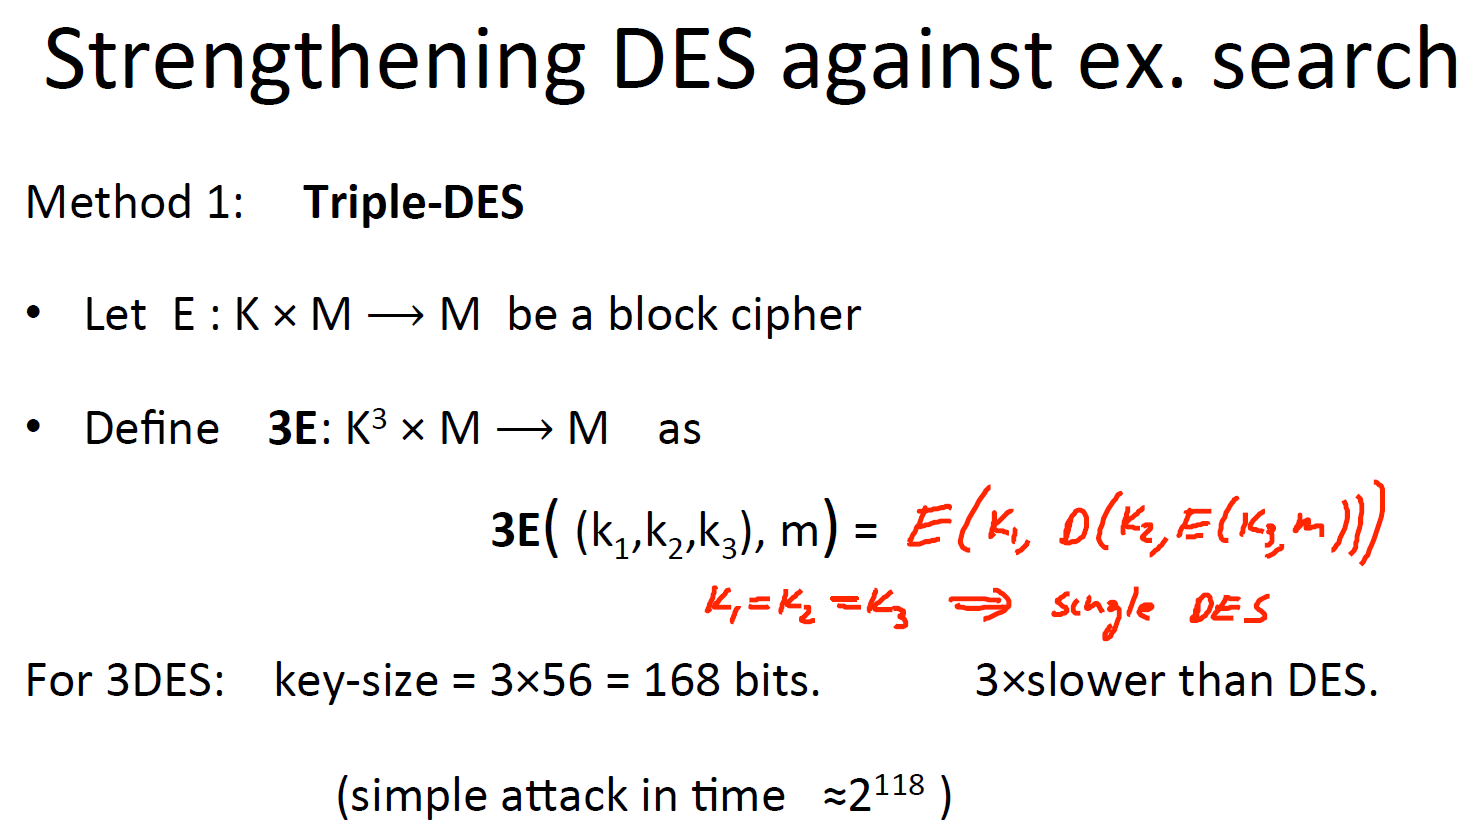
\includegraphics{./Images/3-DES.png}

The Whys?: - In triple DES we first do an Encryption of message block
with key 1, then a decryption with key 2 and again an encryption with
key 3 and all 3 keys are used in the decryption process inversely. Why
did we have a decryption in b/w and not 3 consecutive encryptions? cuz
there exist a possibility that k1 = k2 = k3 and hence what we have is a
single DES but 3 times slower. - Why not use 2-DES, while it also have a
secure \(2^{112}\) key space? Because it is prone to a special kind of
attack known as Meet in the middle attack.

\textbf{You should never ever use your own crypto implementations or
even design a new cipher for delivering security}, due to the following
reason: 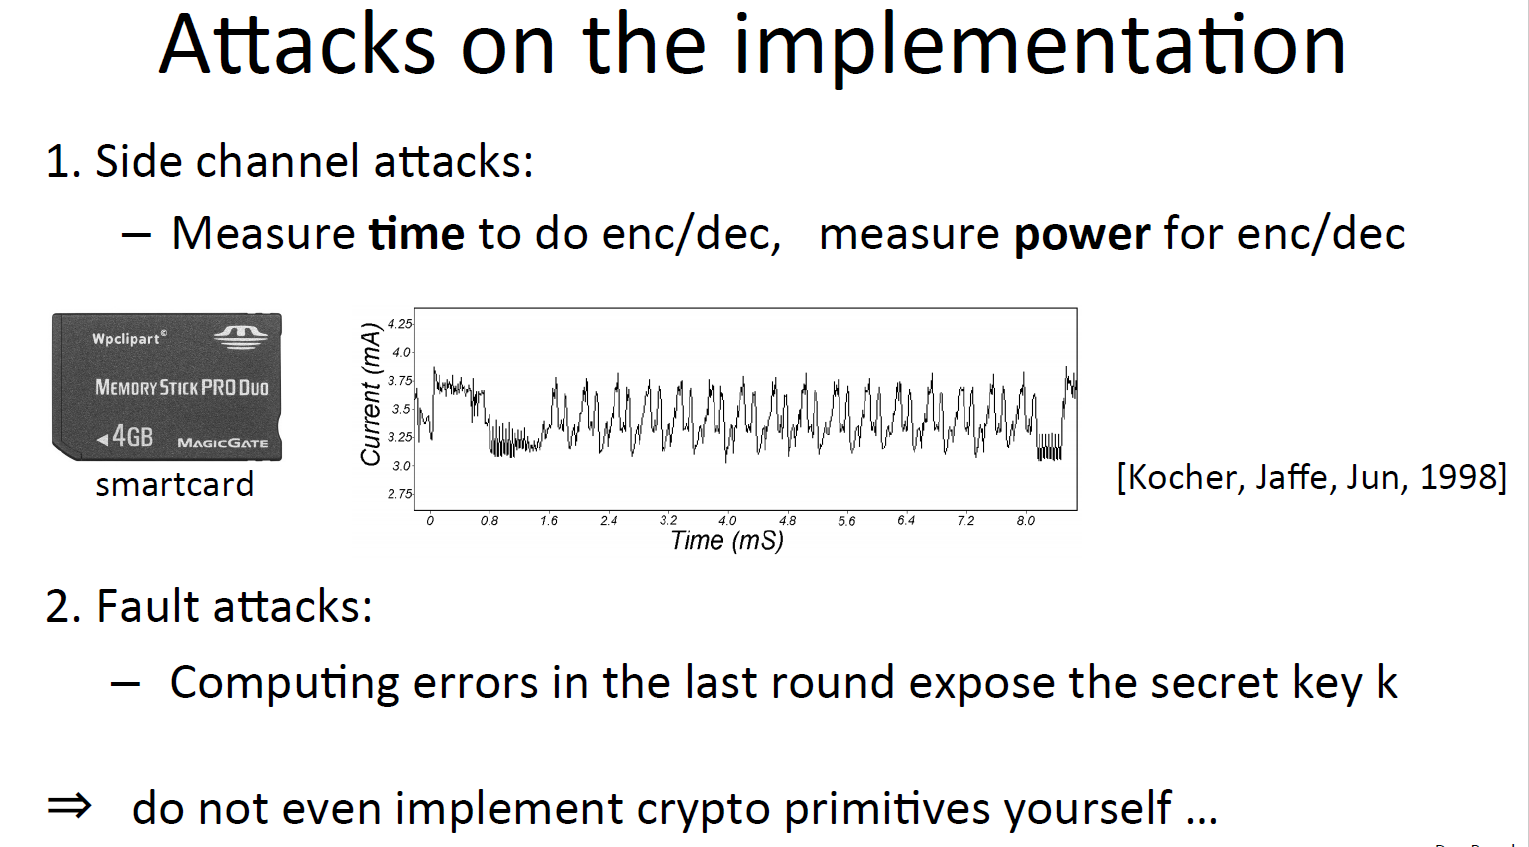
\includegraphics{./Images/ImplementationAttacks.png}

Note: Use a well implemented library instead which take care of these
side channel and fault attacks.

\begin{center}\rule{0.5\linewidth}{\linethickness}\end{center}

    \hypertarget{aes-advanced-encryption-standard}{%
\subsubsection{AES (Advanced Encryption
Standard)}\label{aes-advanced-encryption-standard}}

Recommended Watch:
\href{https://www.coursera.org/learn/crypto/lecture/cHOMl/the-aes-block-cipher}{AES
in Depth}

The more popular and widely adopted symmetric encryption algorithm
likely to be encountered nowadays is the Advanced Encryption Standard
(AES). It is found at least six time faster than triple DES.

A replacement for DES was needed as its key size was too small. With
increasing computing power, it was considered vulnerable against
exhaustive key search attack. Triple DES was designed to overcome this
drawback but it was found slow.

The features of AES are as follows: - Symmetric key symmetric block
cipher - encrypts 128-bit block of data using either 128/192/256-bit
keys - Stronger and faster than Triple-DES

\textbf{Security vs Speed Trade-off:} The larger the key size is, the
more secure the block cipher is as a psuedo random permutation (PRP) but
as it would also have more rounds involve in its operation the slower
the cipher become. Hence, AES-128 is fastest while AES-256 is the most
secure.

\textbf{Foundation of AES} {[}Generic Construction{]}:
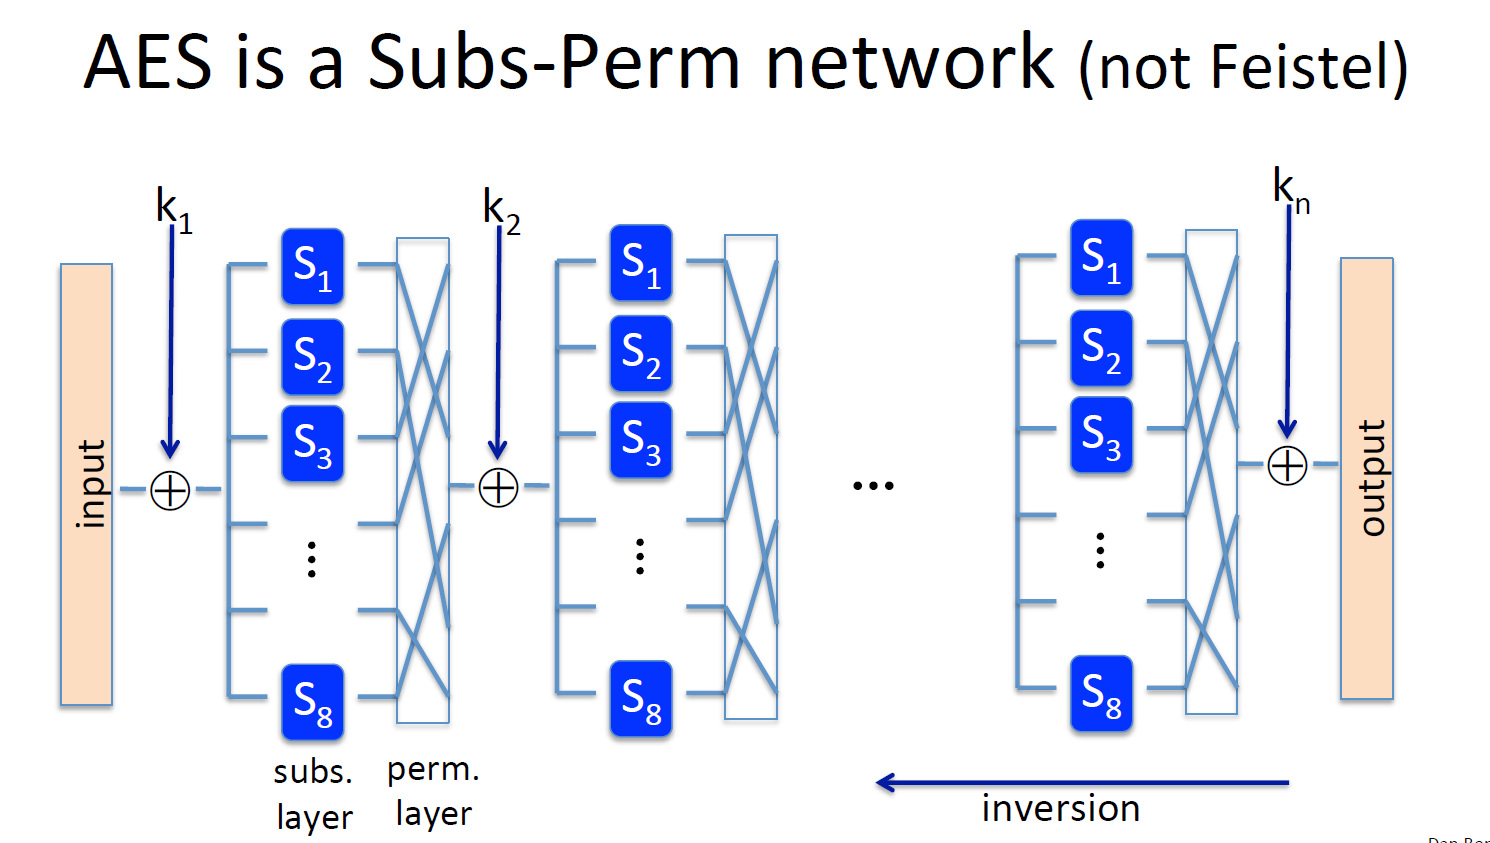
\includegraphics{./Images/AES-Generic.png}

\begin{quote}
AES is built as a \textbf{Substitution Permutation (Subs-Perm) Network}
and not a Feistel network. Note that in a Feistel network only have the
bits are changed from round to round (the left half of the next round
are simply the copy of the right half of the previous round). While in
Subs-Perm network all the bits are changed in every round. AES also uses
the concept of round keys which are derived from 128-bit key space. AES
is built to be completely reversible, otherwise the decryption would
have not been possible, therefore the substitution layers as well the
permutation layers are reversible, i.e., given the ciphertext we can
applying all the steps in AES in reverse order (with the same round
keys) and produce the original text.
\end{quote}

Having a view of the generic construction of the AES, now lets look at
the specifics of AES:

\textbf{AES-128} 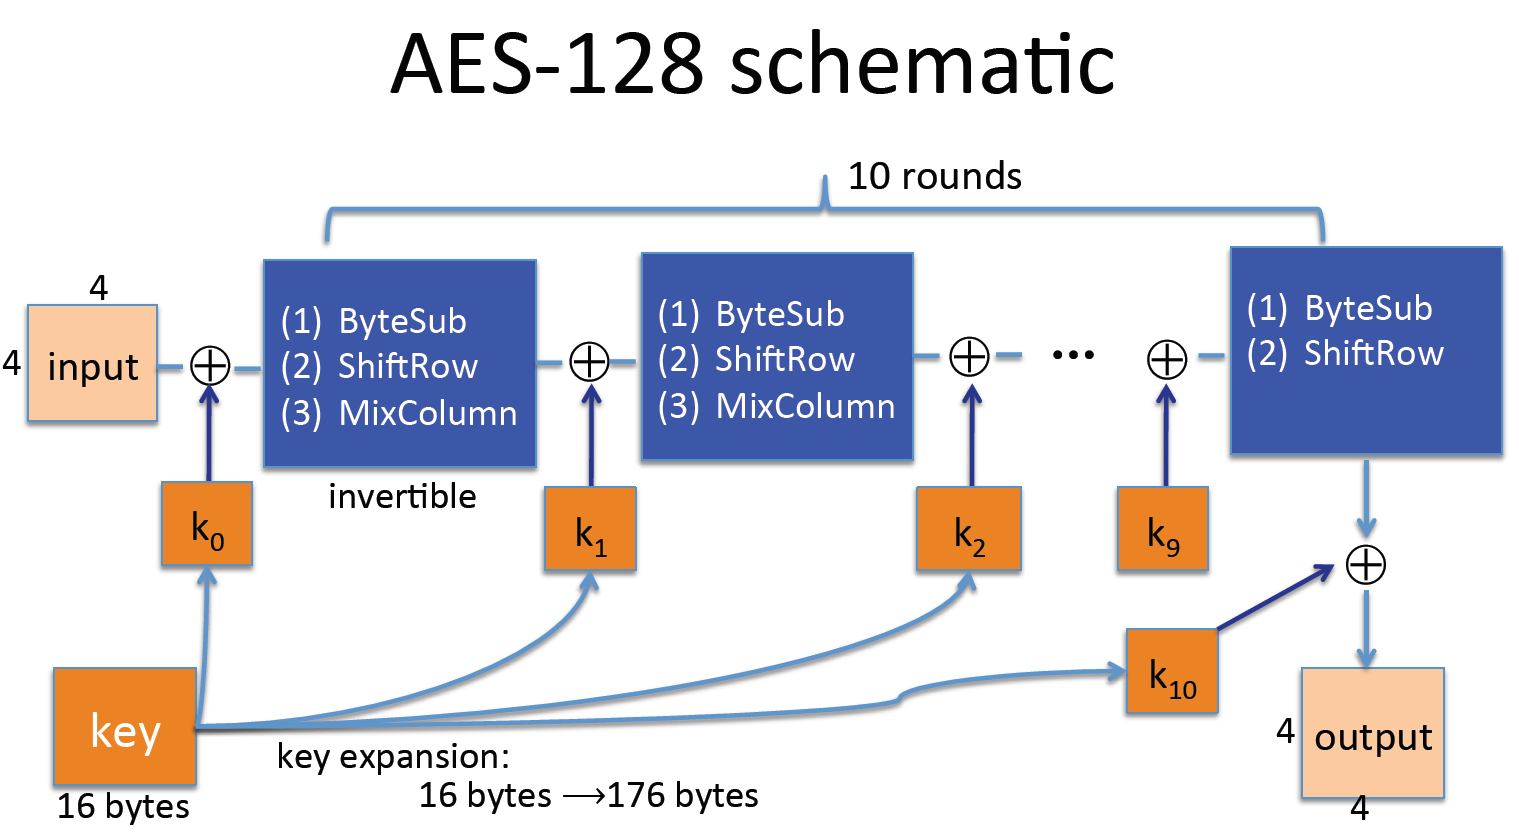
\includegraphics{./Images/AES-128.png}

The Flow(Encryption): 1. AES-128 operates on blocks of 128 bits, hence
we start off with a \(4\times 4\) byte input block (each cell with 1
byte). 2. Then we XOR the input block with a \(4\times 4\) byte block of
round key (which are derived, by expansion, from the 16-byte{[}128{]}
AES key). 3. Then a round function is applied which contains 3
sub-routines, namely Byte Substitution, Shift Row and Mix-Column. 4.
This is done again and again for 10 rounds, but interestingly in the
last round the Mix-column routine is absent. 5. The output, ciphertext,
is the XOR of the last round key and with the output of the last round
function.

Decryption is just the inverse: The process of decryption of an AES
ciphertext is similar to the encryption process in the reverse order.
The round keys are applied in reverse order followed by inverted round
function. Following are the steps, except for the initial round in
reverse order (as it do not contains the mix-column sub-routine) :

\begin{itemize}
\tightlist
\item
  Add round key
\item
  Mix columns
\item
  Shift rows
\item
  Byte substitution
\end{itemize}

The round function:

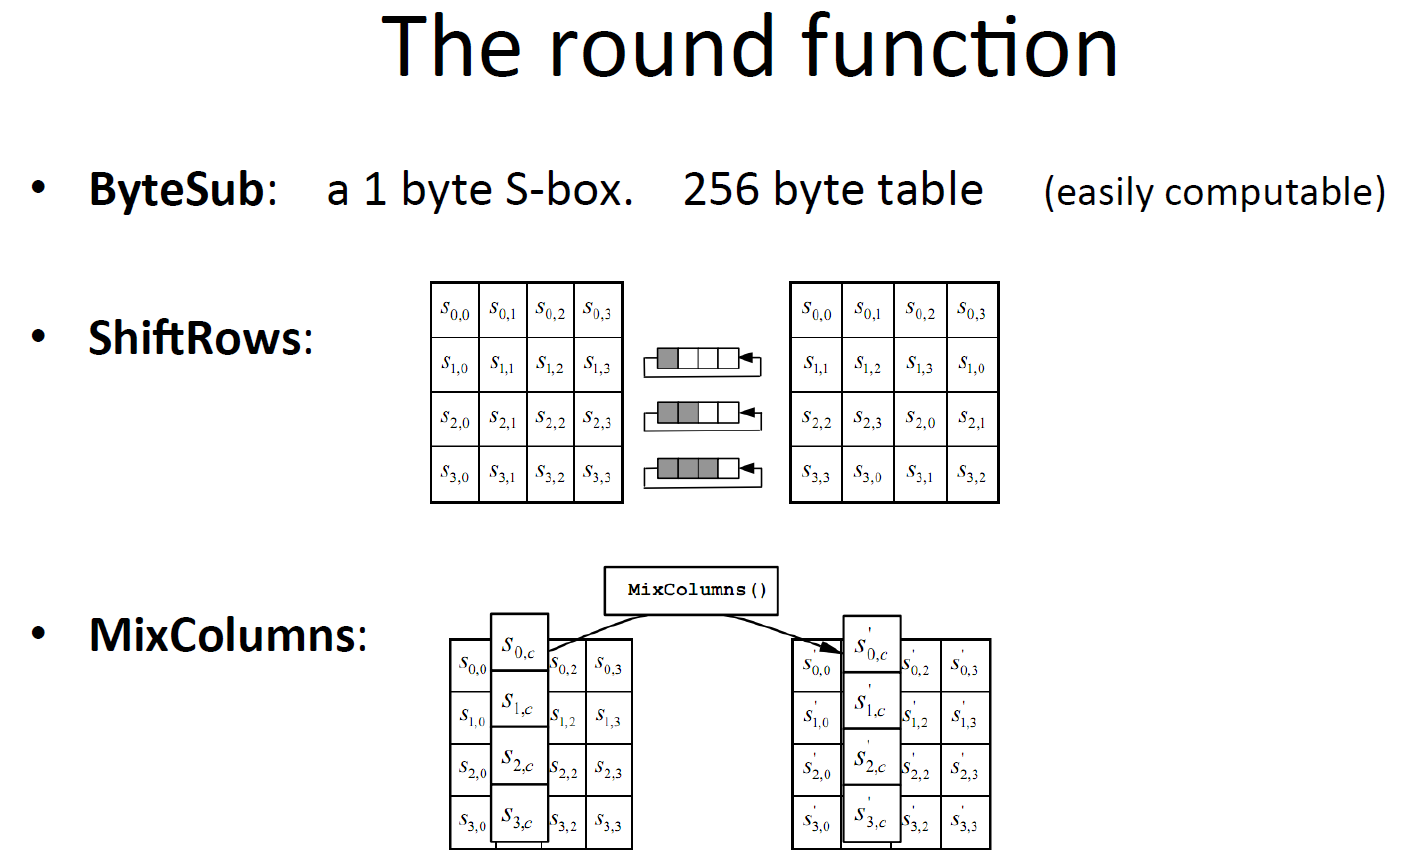
\includegraphics{./Images/AES-Round.png}

Description: - ByteSub: Applies a 256-byte S-box(just a lookup table) to
each byte in the \(4\times 4\) byte message block and outputs a
\(4\times 4\) byte block. - ShiftRows: Applies a cyclic shift to the
rows in the \(4\times 4\) byte block (no shift on the first row) -
MixColumns:Applies linear transformation independently to each column

Note: AES is being used everywhere now as it is easily computable as
well as compact. Even Intel and AMD have integrated AES into their
processors itself.

Attacks on AES: - Best key recovery attack \(2^{124}\): Just 4 times
better than the exhaustive search(\(2^{128}\)) - Related key attack:
Given that we have inp/out pairs from four related keys, key could be
recovered in \(2^{99}\). But it would require related keys while we
chose keys at random.

The above two are the only, non efficient, attacks on AES.

\begin{center}\rule{0.5\linewidth}{\linethickness}\end{center}

    \hypertarget{using-block-ciphers-modes-of-operation}{%
\subsubsection{Using Block Ciphers: Modes of
Operation}\label{using-block-ciphers-modes-of-operation}}

There are other modes of operations (which are not discussed below),
they can be explored at:
\href{https://www.tutorialspoint.com/cryptography/block_cipher_modes_of_operation.htm}{Modes
of Operations}

Suggestion: Don't bother about the inner-working of AES and 3-DES.
Assume both are secure PRPs and we will see how to use them.

\begin{quote}
\textbf{Modes of Operation} are procedural rules for a generic block
cipher. Interestingly, the different modes result in different
properties being achieved which add to the security of the underlying
block cipher.
\end{quote}

A block cipher processes the data blocks of fixed size. Usually, the
size of a message is larger than the block size. Hence, the long message
is divided into a series of sequential message blocks, and the cipher
operates on these blocks one at a time.

\hypertarget{electronic-code-book-ecb-mode}{%
\paragraph{Electronic Code Book (ECB)
Mode}\label{electronic-code-book-ecb-mode}}

Corresponding Watch:
\href{https://www.coursera.org/learn/crypto/lecture/QZAHs/modes-of-operation-one-time-key}{Modes
of Operation: One Time Key} Take a look at the
CryptographyI/LectureSlides/Week 2/UsingBlockCiphers.pdf for more on
ECB.

This mode is a most straightforward way of processing a series of
sequentially listed message blocks.

Operations: - Cipher the first block of plaintext and encrypts it with
the key to produce the first block of ciphertext. - It then takes the
second block of plaintext and follows the same process with same key and
so on so forth.

\begin{quote}
The ECB mode is \textbf{deterministic}, that is, if plaintext block
\(p_{1}\), \(p_{2}\),\ldots{}, \(p_{m}\) are encrypted twice under the
same key (i.e if there exist an identical plaintext \(p_{x}\) =
\(p_{y}\)), the output ciphertext for those blocks will be the same.
Therefore, ECB is terrible as it \textbf{breaks the semantic security}
(the adversary will learn something about the plaintext from the given
ciphertext) given that we have two identical plaintext blocks. Attacks
like CPA (chosen plain text attacks) breaks ECB, hence,\textbf{ECB is
not CPA secure}.
\end{quote}

Bottom line: ECB is not semantically secure for messages that would take
more than one block. More generally, deterministic algorithms aren't
semantically secure (as they output same ciphertext for same plaintext,
hence, allowing the adversary to know that there exist two identical
plaintexts in the message just by analyzing their corresponding,
identical, ciphertexts).

\hypertarget{security-for-many-time-keys-cpa-security}{%
\paragraph{Security for Many Time Keys (CPA
Security):}\label{security-for-many-time-keys-cpa-security}}

For in-depth look:
\href{https://www.coursera.org/learn/crypto/lecture/1pnne/security-for-many-time-key-cpa-security}{Security
for Many Time Keys}

Following represents the Threat Model for Many Time Keys(keys that are
used to encrypt multiple messages):
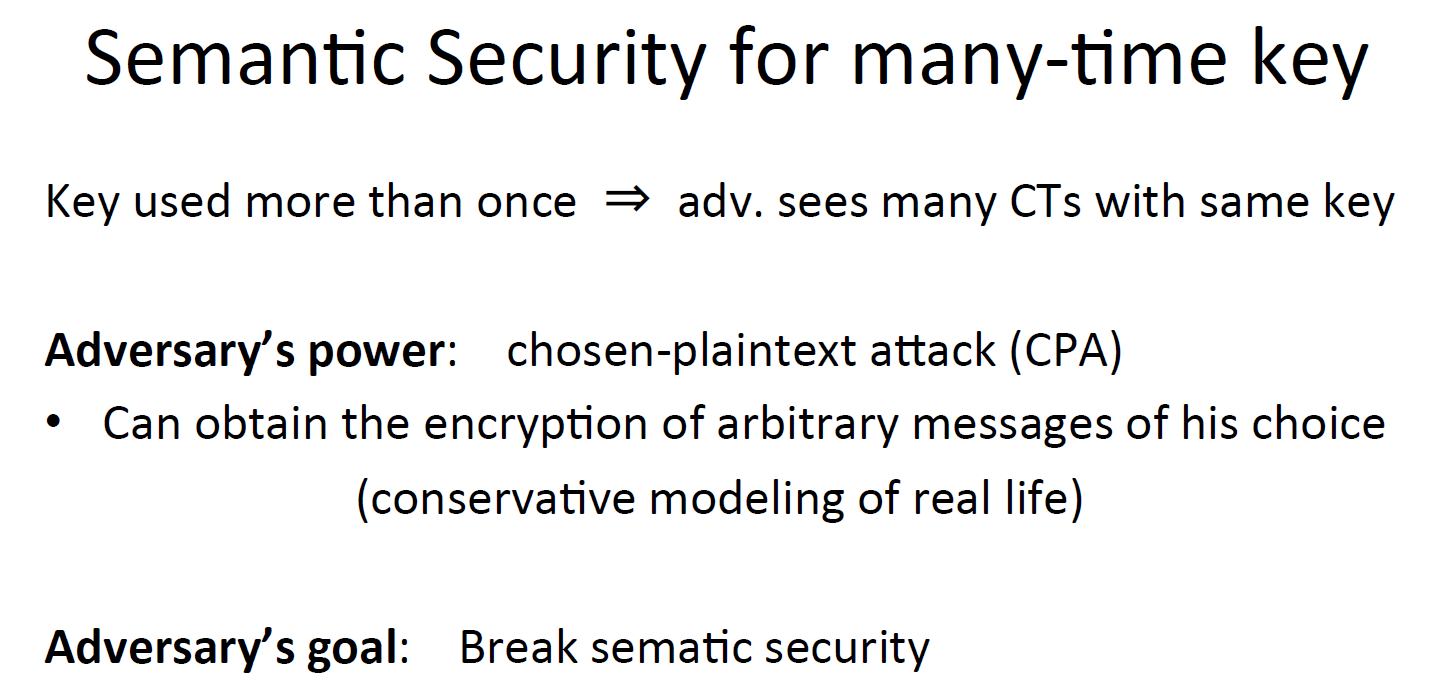
\includegraphics{./Images/SSforManyTimeKeys.png}

Why deterministic ciphers Insecure against CPA(chosen plain text
attack)? 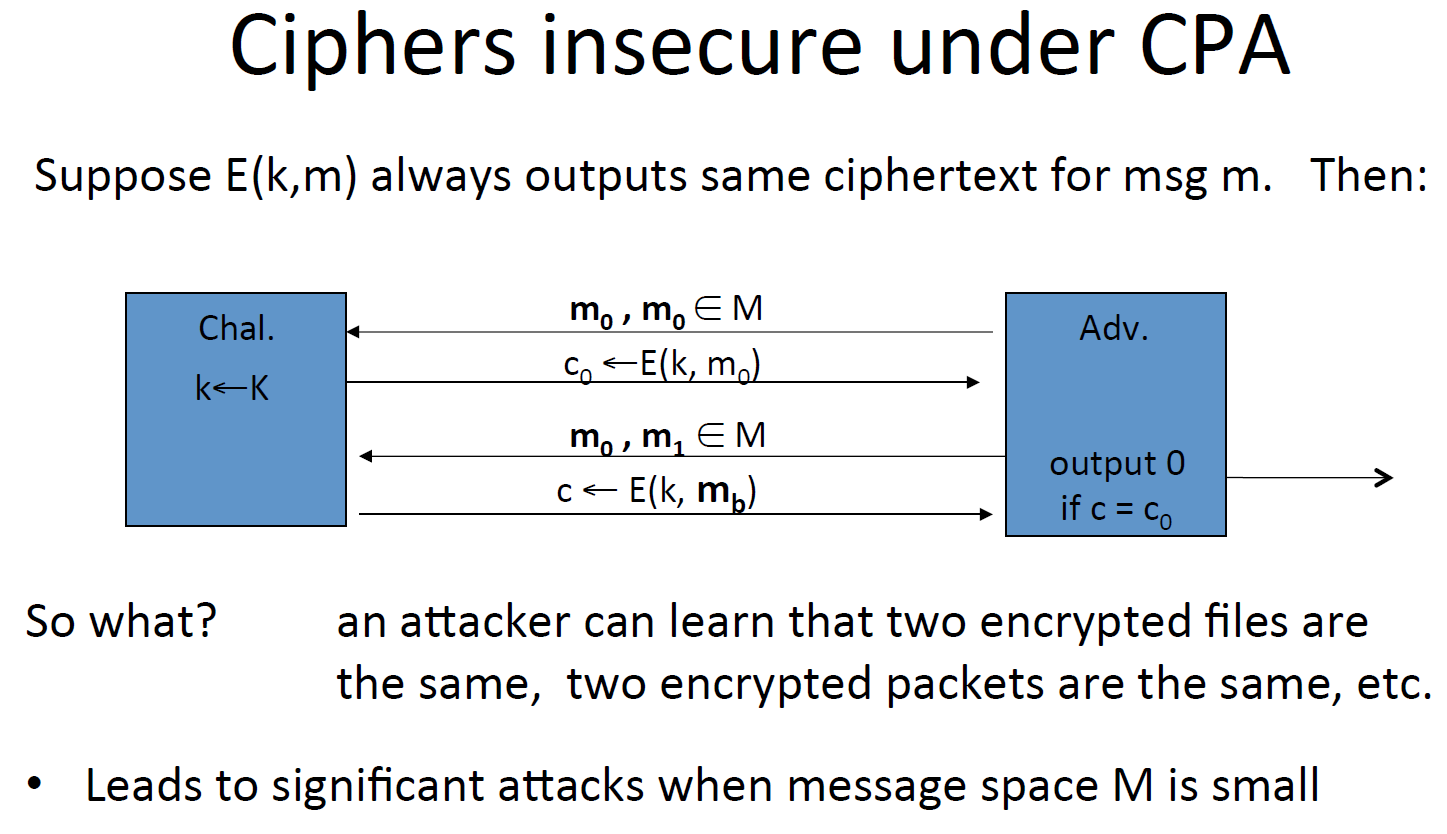
\includegraphics{./Images/DeterministicCiphersInsecure.png}
Description: - The CPA ability allows the attacker to do q
queries/challenges to the cipher. Where as everything else is same as in
the Section \ref{semantic-security} setting. - The cipher is
deterministic and under the same key, it will produce the same
ciphertext given that adversary supplied the same plaintext \(m_{0}\),
so in both the Exp(0) and Exp(1) the ciphertext for \(m_{0}\) will be
returned. - The adversary will again challenge the Cipher (as it can do
it q times), while the cipher is using the same key. Adversary now sends
in \(m_{0}\), \(m_{1}\) and it can accurately tell which ciphertext is
returned (as it already know what is the ciphertext corresponding to
\(m_{0}\) from the previous query). - Hence, the deterministic quality
of the cipher (and that it uses same key for multiple message/query
encryption) coupled with CPA ability of the adversary breaks the
semantic security.

Bottom line: \textbf{Deterministic Encryption cannot be semantically
secure under a Chosen Plaintext Attack (CPA).}

\textbf{What do we require to provide CPA Security?}
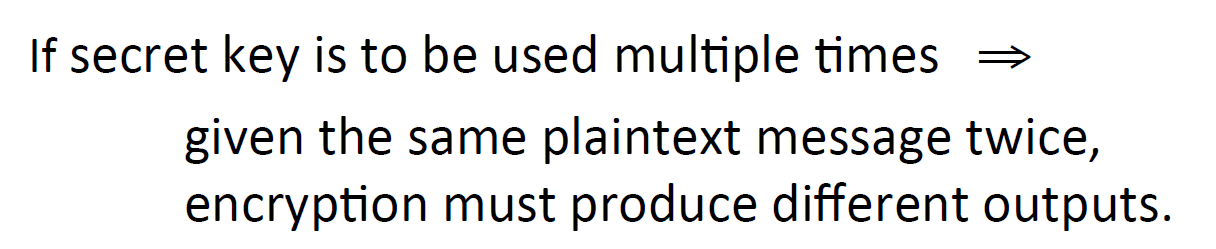
\includegraphics{./Images/RequisiteForCPASecurity.png}

\textbf{Solutions for CPA Security:} - \textbf{Randomized Encryption:}
The Encryption Algorithm chooses some random string and uses that random
string along side the plaintext to generate the ciphertext. This would
allow for the generation of different ciphertexts (blocks) for the same
plaintexts (blocks). Also, the size of the ciphertext is relatively
longer, roughly speaking, \(CT-size = PT-size + #random-bits\) (\#
stands for number of). Note, the random string should be large enough
such that we can use it without repetition of the ciphertext for
multiple encryptions of the same plaintext.

\begin{itemize}
\item
  \textbf{Nonce-Based Encryption:} Here we use a nonce which is a unique
  value such that the pair (k, n) which is used to encrypt message m
  becomes unique and until we keep changing the nonce for encrypting
  even the identical messages with the same key, we will generate a
  unique ciphertext. \includegraphics{./Images/NonceBasedEncryption.png}
\item
  \textbf{Nonce as counter:} Both encryptor and decryptor uses a counter
  for keeping state from mssg to mssg and this counter can be used as a
  nonce as the counter will be a unique value for each mssg and would be
  synced at both ends, therefore could be used as a nonce (no explicit
  nonce would be required). It's a stateful method.
\item
  \textbf{Random Nonce:} Here nonce is a random variable from a Nonce
  Space N, which should be large enough such that there is a really low
  (or negligible) probability of a nonce being repeated in a given key's
  lifetime. This is a stateless method.
\end{itemize}

General definition of Nonce: Nonce is a unique value that doesn't
repeat. It does not have to be random.

\begin{center}\rule{0.5\linewidth}{\linethickness}\end{center}

    \textbf{Discovering the CPA Secure Ciphers {[}There are 2 prominent
Constructions to achieve CPA Security{]}}

\hypertarget{cipher-block-chainingcbc-mode}{%
\paragraph{Cipher Block Chaining(CBC)
Mode}\label{cipher-block-chainingcbc-mode}}

Recommended Watch:
\href{https://www.coursera.org/learn/crypto/lecture/wlIX8/modes-of-operation-many-time-key-cbc}{Cipher
Block Chaining}

\begin{quote}
\textbf{Cipher block chaining (CBC)} is a mode of operation for a block
cipher (one in which a sequence of bits are encrypted as a single unit
or block with a cipher key applied to the entire block). Cipher block
chaining uses what is known as an initialization vector (IV) of a
certain length. One of its key characteristics is that it uses a
chaining mechanism that causes the decryption of a block of ciphertext
to depend on all the preceding ciphertext blocks. As a result, the
entire validity of all preceding blocks is contained in the immediately
previous ciphertext block. A single bit error in a ciphertext block
affects the decryption of all subsequent blocks. Rearrangement of the
order of the ciphertext blocks causes decryption to become corrupted.
Basically, in cipher block chaining, each plaintext block is XORed (see
XOR) with the immediately previous ciphertext block, and then encrypted.
\end{quote}

Note: CBC cannot be parallelized as it is inherently sequential.

\textbf{How \(AES_{CBC}\) is CPA secure (Semantically secure under
CPA)?} Identical ciphertext blocks can only result if the same plaintext
block is encrypted using both the same key and the initialization
vector, and if the ciphertext block order is not changed. It has the
advantage over the Electronic Code Book mode in that the XOR'ing process
hides plaintext patterns. Ideally, the initialization vector should be
different for any two messages encrypted with the same key.

\textbf{Construction 1: CBC with rand IV}
\includegraphics{./Images/CBC-1.png}

The Flow: \(E_{CBC}\) is the our AES encryption scheme using the CBC
mode of operation. When it's asked to encrypt a message m, the first
thing it's going to do is it's going to choose a random IV
(Initialization) that's exactly one block of the block cipher. So IV is
one cypher block. So in the case of AES the IV would be 16 bytes (128
bits). And then we're gonna run through the algorithm here:

The IV basically that we chose is gonna be XORed to the first plain text
block. And then the result is gonna be encrypted using the AES block
cipher and output the first block of the ciphertext. And now comes the
chaining part where we actually use the first block of the ciphertext to
kind of mask the second block of the plaintext. So we XOR the two
together and the encryption of that becomes the second ciphertext block.
And so on, and so on, and so forth. So this is cIpher block chaining,
you can see that each cipher block is chained and XORed into the next
plaintext block, and the final ciphertext is going to be essentially the
initial IV that we chose along with all the ciphertext blocks.

\textbf{Initialization Vector:} IV stands for Initialization Vector. And
we're going to be seeing that term used quite a bit, every time we need
to pick something at random at the beginning of the encryption scheme
typically we'll call that an IV for initialization vector. So you notice
that the \textbf{ciphertext is a little bit longer than the plaintext}
because we had to include this IV in the ciphertexts which basically
captures the randomness that was used during encryption.

\textbf{CBC Construction 1{[}Decryption{]}:}
\includegraphics{./Images/CBC-1Decrypt.png}

\textbf{CBC - CPA Analysis:} So the following theorem is going to show
that in fact CBC mode encryption with a random IV is in fact
semantically secure under a chosen plaintext attack.
\includegraphics{./Images/CBC-CPA-Analysis.png} So let's take it more
precisely, basically if we start with a PRP, in other words, our block
cipher E, that is defined over a space X, then we are gonna to end up
with a encryption algorithm \(E_{CBC}\) that takes messages of length L
and outputs ciphertexts of length L+1. And then suppose we have an
adversary that makes q chosen plaintext queries.

Then we can state the following security fact, that for every such
adversary that's attacking \(E_{CBC}\), to exist an adversary that's
attacking the PRP, the block cipher, with the following relation between
the two algorithms: the advantage of algorithm A against the encryption
scheme is less than the advantage of algorithm B against the original
PRP plus some noise term. So lets interpret this theorem, so what this
means is that essentially since E is a secure PRP \(Adv_{PRP}\){[}B,
E{]} is negligible, and our goal is to say that adversary A's advantage
is also negligible. However, here we are prevented from saying that
because we got this extra error term. This is often called an error term
and to argue that CBC is secure we have to make sure that the error term
is also negligible. Because if both of these terms on the right are
negligible, there sum is negligible and therefore the advantage of A
against \(E_{CBC}\) would also be negligible.

So this says that in fact for \(E_{CBC}\) to be secure it has better be
the case that \(q^{2}\).\(l^{2}\) is much, much, much smaller than the
value X, where L is simply the length of the messages that we're
encrypting (so L could be like say a 1000, which means that we are
encrypting messages that are at most 1000 AES blocks) and q is the
number of ciphertexts that the adversary gets to see under the CPA
attack, but in real life what q is, is basically the number of times
that we have used the key K to encrypt messages.

Example: \includegraphics{./Images/CBC-CPA-Ex.png} Note: Using the given
Adv formulation, we are able to precisely calculate after how many
encryptions {[}and therefore after how many bytes of encryption{]}, here
in AES-128 it's \(2^{48}\)blocks, we must change the key.

Warning: CBC where attacker can predict the IV is not CPA-secure!!.
Hence, it's crucial that the IV be random and not predictable.

\textbf{Construction 1': Nonce Based CBC}

\includegraphics{./Images/NonceBasedCBC.png}

Description: This is a nonce based version of the CBC where the IV is
replaced by a nonce (if the nonce is already known to the recipient, ex:
counter nonce, then we don't need to include the nonce explicitly in the
ciphertext, so ciphertext is exactly the same as the plaintext).

If the nonce is random then we don't need the below explained extra step
(we can use it directly to XOR with the initial plaintext block).

However, it's perfectly fine to use a non random unique nonce, however,
it's absolutely crucial to know that if we do this then we would have to
take an \textbf{extra step} before using the nonce in the CBC chain,
that is: \textbf{to first encrypt the nonce using a key \(k_{1}\)}
(which is different from the key, k, that is used in the rest of the
mechanism) \textbf{so that the output is going to be a random IV which
is then used in the CBC chain.} So, this extra step is extremely crucial
without CBC mode encryption with nonce wouldn't be CPA secure. Note: Key
\(k_{1}\) could not be equal to key k, as that would also not be CPA
secure.

Example of a Cyrto API {[}AES-CBC with rand IV{]}:
\includegraphics{./Images/ExampleCryptoAPI.png}

\hypertarget{implementation-of-aes-cbc-with-random-iv-using-pycrypto-api}{%
\subsubsection{Implementation of AES (CBC with random IV) using PyCrypto
API}\label{implementation-of-aes-cbc-with-random-iv-using-pycrypto-api}}

    \begin{Verbatim}[commandchars=\\\{\}]
{\color{incolor}In [{\color{incolor}1}]:} \PY{k+kn}{from} \PY{n+nn}{Crypto}\PY{n+nn}{.}\PY{n+nn}{Cipher} \PY{k}{import} \PY{n}{AES}
        \PY{k+kn}{import} \PY{n+nn}{random}\PY{o}{,} \PY{n+nn}{string}
        
        \PY{k}{def} \PY{n+nf}{split\PYZus{}txt}\PY{p}{(}\PY{n}{text}\PY{p}{,} \PY{n}{splitter}\PY{p}{)}\PY{p}{:}
            \PY{l+s+s2}{\PYZdq{}}\PY{l+s+s2}{Constructs the splitted\PYZus{}text [Block\PYZhy{}size division]}\PY{l+s+s2}{\PYZdq{}}
             
            \PY{k}{if} \PY{n+nb}{len}\PY{p}{(}\PY{n}{text}\PY{p}{)}\PY{o}{\PYZpc{}}\PY{k}{splitter} == 0:
                \PY{n}{extras} \PY{o}{=} \PY{l+m+mi}{0}
                \PY{n}{splitted\PYZus{}text} \PY{o}{=} \PY{p}{[}\PY{n}{text}\PY{p}{[}\PY{n}{start}\PY{p}{:} \PY{n}{start}\PY{o}{+}\PY{n}{splitter}\PY{p}{]} \PY{k}{for} \PY{n}{start} \PY{o+ow}{in} \PY{n+nb}{range}\PY{p}{(}\PY{l+m+mi}{0}\PY{p}{,} \PY{n+nb}{len}\PY{p}{(}\PY{n}{text}\PY{p}{)}\PY{p}{,} \PY{n}{splitter}\PY{p}{)}\PY{p}{]}
            \PY{k}{else}\PY{p}{:}
                \PY{n}{extras} \PY{o}{=} \PY{n}{splitter} \PY{o}{\PYZhy{}} \PY{n+nb}{len}\PY{p}{(}\PY{n}{text}\PY{p}{)}\PY{o}{\PYZpc{}}\PY{k}{splitter}
                \PY{n}{text} \PY{o}{=} \PY{n}{text} \PY{o}{+} \PY{n}{random\PYZus{}generator}\PY{p}{(}\PY{n}{extras}\PY{p}{)}
                \PY{n}{splitted\PYZus{}text} \PY{o}{=} \PY{p}{[}\PY{n}{text}\PY{p}{[}\PY{n}{start}\PY{p}{:} \PY{n}{start}\PY{o}{+}\PY{n}{splitter}\PY{p}{]} \PY{k}{for} \PY{n}{start} \PY{o+ow}{in} \PY{n+nb}{range}\PY{p}{(}\PY{l+m+mi}{0}\PY{p}{,} \PY{n+nb}{len}\PY{p}{(}\PY{n}{text}\PY{p}{)}\PY{p}{,} \PY{n}{splitter}\PY{p}{)}\PY{p}{]}
            \PY{k}{return} \PY{n}{splitted\PYZus{}text}\PY{p}{,} \PY{n}{extras}
        
        \PY{k}{def} \PY{n+nf}{random\PYZus{}generator}\PY{p}{(}\PY{n}{n}\PY{p}{)}\PY{p}{:} 
            \PY{l+s+s2}{\PYZdq{}}\PY{l+s+s2}{Generates n random characters for padding}\PY{l+s+s2}{\PYZdq{}}
                
            \PY{k}{return} \PY{l+s+s1}{\PYZsq{}}\PY{l+s+s1}{\PYZsq{}}\PY{o}{.}\PY{n}{join}\PY{p}{(}\PY{n}{random}\PY{o}{.}\PY{n}{choice}\PY{p}{(}\PY{n}{string}\PY{o}{.}\PY{n}{ascii\PYZus{}letters}\PY{p}{)} \PY{k}{for} \PY{n}{x} \PY{o+ow}{in} \PY{n+nb}{range}\PY{p}{(}\PY{n}{n}\PY{p}{)}\PY{p}{)}
        
        
        \PY{k}{def} \PY{n+nf}{encryption}\PY{p}{(}\PY{n}{key}\PY{p}{,} \PY{n}{IV}\PY{p}{)}\PY{p}{:}
            \PY{l+s+s2}{\PYZdq{}}\PY{l+s+s2}{AES Encryption Scheme}\PY{l+s+s2}{\PYZdq{}}
            
            \PY{n}{block\PYZus{}size} \PY{o}{=} \PY{n+nb}{len}\PY{p}{(}\PY{n}{key}\PY{p}{)}
            \PY{n}{obj} \PY{o}{=} \PY{n}{AES}\PY{o}{.}\PY{n}{new}\PY{p}{(}\PY{n}{key} \PY{p}{,} \PY{n}{AES}\PY{o}{.}\PY{n}{MODE\PYZus{}CBC}\PY{p}{,} \PY{n}{IV}\PY{p}{)}
            \PY{n}{message} \PY{o}{=} \PY{n+nb}{input}\PY{p}{(}\PY{l+s+s1}{\PYZsq{}}\PY{l+s+s1}{Please enter the message to be encrypted: }\PY{l+s+s1}{\PYZsq{}}\PY{p}{)}
            \PY{n+nb}{print}\PY{p}{(}\PY{l+s+s1}{\PYZsq{}}\PY{l+s+se}{\PYZbs{}n}\PY{l+s+s1}{Encrypting...}\PY{l+s+s1}{\PYZsq{}}\PY{p}{)}
            \PY{n}{splitted\PYZus{}text}\PY{p}{,} \PY{n}{extras} \PY{o}{=} \PY{n}{split\PYZus{}txt}\PY{p}{(}\PY{n}{message}\PY{p}{,} \PY{n}{block\PYZus{}size}\PY{p}{)}
            \PY{n}{ciphertexts} \PY{o}{=} \PY{p}{[}\PY{p}{]}
            \PY{k}{for} \PY{n}{text} \PY{o+ow}{in} \PY{n}{splitted\PYZus{}text}\PY{p}{:}
                \PY{n}{ciphertexts}\PY{o}{.}\PY{n}{append}\PY{p}{(}\PY{p}{(}\PY{n}{obj}\PY{o}{.}\PY{n}{encrypt}\PY{p}{(}\PY{n}{text}\PY{p}{)}\PY{p}{)}\PY{p}{)}
            \PY{k}{return} \PY{n}{ciphertexts}\PY{p}{,}\PY{n}{extras}
        
        \PY{k}{def} \PY{n+nf}{decryption}\PY{p}{(}\PY{n}{key}\PY{p}{,} \PY{n}{IV}\PY{p}{,} \PY{n}{ciphertexts}\PY{p}{,} \PY{n}{extras}\PY{p}{)}\PY{p}{:}
            \PY{l+s+s2}{\PYZdq{}}\PY{l+s+s2}{AES Decryption Scheme}\PY{l+s+s2}{\PYZdq{}}
            
            \PY{n+nb}{print}\PY{p}{(}\PY{l+s+s1}{\PYZsq{}}\PY{l+s+s1}{Decrypting...}\PY{l+s+s1}{\PYZsq{}}\PY{p}{)}
            \PY{n}{obj2} \PY{o}{=} \PY{n}{AES}\PY{o}{.}\PY{n}{new}\PY{p}{(}\PY{n}{key}\PY{p}{,} \PY{n}{AES}\PY{o}{.}\PY{n}{MODE\PYZus{}CBC}\PY{p}{,} \PY{n}{IV}\PY{p}{)}
            \PY{n}{original\PYZus{}mssgs} \PY{o}{=} \PY{p}{[}\PY{p}{]}
            \PY{k}{for} \PY{n}{index} \PY{o+ow}{in} \PY{n+nb}{range}\PY{p}{(}\PY{n+nb}{len}\PY{p}{(}\PY{n}{ciphertexts}\PY{p}{)}\PY{p}{)}\PY{p}{:}
                    \PY{n}{original\PYZus{}mssgs}\PY{o}{.}\PY{n}{append}\PY{p}{(}\PY{n}{obj2}\PY{o}{.}\PY{n}{decrypt}\PY{p}{(}\PY{n}{ciphertexts}\PY{p}{[}\PY{n}{index}\PY{p}{]}\PY{p}{)}\PY{p}{)}
        
            \PY{n}{original\PYZus{}mssgs} \PY{o}{=} \PY{n+nb}{list}\PY{p}{(}\PY{n+nb}{map}\PY{p}{(}\PY{k}{lambda} \PY{n}{x}\PY{p}{:} \PY{n}{x}\PY{o}{.}\PY{n}{decode}\PY{p}{(}\PY{l+s+s2}{\PYZdq{}}\PY{l+s+s2}{utf\PYZhy{}8}\PY{l+s+s2}{\PYZdq{}}\PY{p}{)}\PY{p}{,} \PY{n}{original\PYZus{}mssgs}\PY{p}{)}\PY{p}{)}
            \PY{n}{original\PYZus{}mssgs}\PY{p}{[}\PY{o}{\PYZhy{}}\PY{l+m+mi}{1}\PY{p}{]} \PY{o}{=} \PY{n}{original\PYZus{}mssgs}\PY{p}{[}\PY{o}{\PYZhy{}}\PY{l+m+mi}{1}\PY{p}{]}\PY{p}{[}\PY{p}{:}\PY{o}{\PYZhy{}}\PY{n}{extras}\PY{p}{]}
            \PY{k}{return} \PY{l+s+s1}{\PYZsq{}}\PY{l+s+s1}{\PYZsq{}}\PY{o}{.}\PY{n}{join}\PY{p}{(}\PY{n}{original\PYZus{}mssgs}\PY{p}{)}
        
        \PY{k}{def} \PY{n+nf}{AES\PYZus{}fxn}\PY{p}{(}\PY{p}{)}\PY{p}{:}
            \PY{n}{key} \PY{o}{=} \PY{n+nb}{input}\PY{p}{(}\PY{l+s+s1}{\PYZsq{}}\PY{l+s+s1}{Enter the key [16, 24, 32byte long (here each char is 1 byte)]: }\PY{l+s+s1}{\PYZsq{}}\PY{p}{)}
            \PY{n}{IV}  \PY{o}{=}  \PY{n+nb}{input}\PY{p}{(}\PY{l+s+s1}{\PYZsq{}}\PY{l+s+s1}{Enter the IV [corresponding to the size of the key]: }\PY{l+s+s1}{\PYZsq{}}\PY{p}{)}
            \PY{k}{assert} \PY{n+nb}{len}\PY{p}{(}\PY{n}{key}\PY{p}{)} \PY{o+ow}{in} \PY{p}{[}\PY{l+m+mi}{16}\PY{p}{,} \PY{l+m+mi}{24}\PY{p}{,} \PY{l+m+mi}{32}\PY{p}{]}\PY{p}{,} \PY{l+s+s2}{\PYZdq{}}\PY{l+s+s2}{AES key must be either 16, 24, or 32 bytes long}\PY{l+s+s2}{\PYZdq{}}
            \PY{k}{assert} \PY{n+nb}{len}\PY{p}{(}\PY{n}{IV}\PY{p}{)}  \PY{o+ow}{in} \PY{p}{[}\PY{l+m+mi}{16}\PY{p}{,} \PY{l+m+mi}{24}\PY{p}{,} \PY{l+m+mi}{32}\PY{p}{]}\PY{p}{,} \PY{l+s+s2}{\PYZdq{}}\PY{l+s+s2}{AES IV must be of the same size as the key}\PY{l+s+s2}{\PYZdq{}}
            
            \PY{n}{ciphertexts}\PY{p}{,} \PY{n}{extras} \PY{o}{=} \PY{n}{encryption}\PY{p}{(}\PY{n}{key}\PY{p}{,} \PY{n}{IV}\PY{p}{)}
            \PY{n+nb}{print}\PY{p}{(}\PY{l+s+s1}{\PYZsq{}}\PY{l+s+s1}{Ciphertext: }\PY{l+s+si}{\PYZob{}\PYZcb{}}\PY{l+s+se}{\PYZbs{}n}\PY{l+s+s1}{\PYZsq{}}\PY{o}{.}\PY{n}{format}\PY{p}{(}\PY{l+s+s2}{\PYZdq{}}\PY{l+s+s2}{\PYZdq{}}\PY{o}{.}\PY{n}{join}\PY{p}{(}\PY{n+nb}{map}\PY{p}{(}\PY{n+nb}{str}\PY{p}{,} \PY{n}{ciphertexts}\PY{p}{)}\PY{p}{)}\PY{p}{)}\PY{p}{)}
            \PY{n}{original\PYZus{}mssg} \PY{o}{=} \PY{n}{decryption}\PY{p}{(}\PY{n}{key}\PY{p}{,} \PY{n}{IV}\PY{p}{,} \PY{n}{ciphertexts}\PY{p}{,} \PY{n}{extras}\PY{p}{)}
            \PY{n+nb}{print}\PY{p}{(}\PY{l+s+s1}{\PYZsq{}}\PY{l+s+s1}{Plaintext: }\PY{l+s+si}{\PYZob{}\PYZcb{}}\PY{l+s+s1}{\PYZsq{}}\PY{o}{.}\PY{n}{format}\PY{p}{(}\PY{n}{original\PYZus{}mssg}\PY{p}{)}\PY{p}{)}
            
        \PY{n}{AES\PYZus{}fxn}\PY{p}{(}\PY{p}{)}
\end{Verbatim}

    \begin{Verbatim}[commandchars=\\\{\}]
Enter the key [16, 24, 32byte long (here each char is 1 byte)]: Awesome Crypto!!
Enter the IV [corresponding to the size of the key]: This is 16-B IV!
Please enter the message to be encrypted: Here is a basic implementation of the Advanced Encryption Standard.

Encrypting{\ldots}
Ciphertext: b'\textbackslash{}x7f\textbackslash{}x08\textbackslash{}xa0\textbackslash{}x10\textbackslash{}xd1l\textbackslash{}xa3\textbackslash{}xe5\textbackslash{}xc7x\textbackslash{}x98\textbackslash{}xe1\textbackslash{}xf1\textbackslash{}xf5\textbackslash{}x90H'b'\textbackslash{}x8f\textbackslash{}xd3 g\textbackslash{}x80\textbackslash{}xca\textbackslash{}r\textbackslash{}x11\textbackslash{}xb6\textbackslash{}x9d9\textbackslash{}xd1\textbackslash{}xfc\textbackslash{}xa5t\textbackslash{}xd7'b"h\textbackslash{}x88\textbackslash{}xef\textbackslash{}xf1S\textbackslash{}x8a\textbackslash{}xea\textbackslash{}x8f.\textbackslash{}xcb/\textbackslash{}xc3h\textbackslash{}xff'\textbackslash{}x1d"b'\textbackslash{}xd2\textbackslash{}xbc\textbackslash{}x80=S\textbackslash{}xda\#\textbackslash{}x8dI\textbackslash{}x0e\textbackslash{}xa2\textbackslash{}xeb\textbackslash{}x1b\textbackslash{}xd5F\textbackslash{}x8a'b'\textbackslash{}x1b\textbackslash{}xf6\textbackslash{}x1f\textbackslash{}x9dSn\^{}\textbackslash{}xf1\textbackslash{}x9b\textbackslash{}x0ei\textbackslash{}x19\&\textbackslash{}x80\textbackslash{}x0f\textbackslash{}x1d'

Decrypting{\ldots}
Plaintext: Here is a basic implementation of the Advanced Encryption Standard.

    \end{Verbatim}

    \hypertarget{counter-ctr-mode}{%
\paragraph{Counter (CTR) Mode}\label{counter-ctr-mode}}

CTR mode is method to achieve CPA security, it is actually superior to
CBC and is also referred to as randomized counter mode. Unlike CBC,
randomized counter mode uses a secure PRF. It doesn't need a block
cypher (PRP). It's enough for counter mode to just use a PRF because
we're never going to be inverting this function F. So we're going to let
F be the secure PRF and it acts on N byte blocks. Again if we use AES, N
will be 128.

\textbf{Construction 2: Random Counter Mode}
\includegraphics{./Images/CounterMode.png}

Work Flow: The way the encryption algorithm works in counter mode is it
starts off by choosing a random IV, that's 128 bytes random IV in the
case of AES, and the essentially we start counting. From this random IV,
so you notice the first encryption is of IV then IV+1 up to IV+L. So we
generate this random pad. We XOR the result with the message, and that
gives us the cipher text. And, as usual, you notice that the IV here is
included along with the cipher text.

So that, in fact, the cipher text is a little longer than the original
plain text. And the point, of course, is that, encryption algorithm
chooses a new IV for every message. And so even if I encrypt the same
message twice, I'm gonna get different resulting cipher texts. One thing
to notice that this mode is completely paralyzable, unlike CBC. CBC was
sequential. Hence, if you have three AES engines encryption basically
will work three times as fast. So that's the beauty of counter mode.

\textbf{Construction 2': Nonce Counter Mode}
\includegraphics{./Images/CounterMode-2.png}

Description: Counter mode also has a corresponding nonce based counter
mode. Where the IV is not truly random, but rather, is just a nonce
which could be a counter. And the way you would implement nonce based
counter mode is: - you would take the 128 bits block that used in AES.
And then you would split it in two. - You would use the left 64 bits as
the nonce. - And then once you specify the nonce, the lower order, 64
bits, would be doing the counting inside of the counter modes
encryption. - So nonce goes on the left, and the counter mode encryption
counter goes on the right.

And it's perfectly fine if this nonce is unpredictable. The only
restriction is that you encrypt at most \(2^{64}\) blocks using one
particular nonce. The danger is that you don't want the right side
counter to reset to zero (that's what will happen after \(2^{64}\) block
encryption), then, you will have two blocks that are encrypted using the
same one time pad. Therefore, we should change the block, after
\(2^{64}\) blocks, to avoid two time pading.

\textbf{Counter mode - CPA Analysis}
\includegraphics{./Images/Counter-CPA-Analysis.png}

Description: Everything is same as that of CBC Analysis, with just the
following exceptions: - In counter mode, we use a secure PRF instead of
a secure PRP. - Counter mode is secure as long as \(q^{2}l\) is
\textless{}\textless{} \textbar{}X\textbar{}, which is better than that
of CBC (\(q^{2}l^{2}\) \textless{}\textless{} \textbar{}X\textbar{}).
Which means that we can encrypt more blocks using AES in counter mode as
compared to AES in CBC.

Example: \includegraphics{./Images/Counter-CPA-Ex.png} Note: We can
encrypt \(2^{64}\) blocks in counter mode without the requirement of
changing the key which is much better that \(2^{48}\) blocks in CBC.

\hypertarget{counter-mode-vs-cipher-block-chaining}{%
\paragraph{Counter Mode vs Cipher Block
Chaining}\label{counter-mode-vs-cipher-block-chaining}}

\includegraphics{./Images/CounterVsCBC.png}

A quick comparison of counter mode and CBC unveils that \textbf{in every
single aspect, counter mode is superior to CBC} with parallelizability
and ability to encrypt more blocks with the same key being the major
advantages of counter mode. And that's actually why most modern
encryption schemes actually are starting to migrate to counter mode, and
abandon CBC. Even though CBC is still quite widely used.

 \#\#\# Summarizing the Block Ciphers
\includegraphics{./Images/BlockCipherSummary.png}

The security notions discussed up to here only provides security against
eavesdropping(\textbf{provides confidentiality}) but not against
tampering. And \textbf{because neither one is designed to defend against
tampering, neither one provides data integrity. And we're going to see
this as a real problem. As a result, in fact, these modes actually
should never, ever be used. You should only be using these modes in
addition to an integrity mechanism.}

\begin{center}\rule{0.5\linewidth}{\linethickness}\end{center}

    \hypertarget{mac-message-authentication-code}{%
\subsubsection{MAC (Message Authentication
Code)}\label{mac-message-authentication-code}}

Corresponding Watch:
\href{https://www.coursera.org/learn/crypto/lecture/iVGR5/message-authentication-codes}{MAC}

A Message Authentication Code (MAC) is a cryptographic primitive used
to: - Provide \textbf{Data Integrity} by allowing verifiers (who also
possess the secret key) to detect any changes to the message content. -
\textbf{Authenticate} a message, in other words, to confirm that the
message came from the stated sender (its authenticity).

Note: MAC do not provide, standalone, confidentiality services.

Here we have, Alice and Bob. They have a shared key, K, which is not
known to the attacker, but known to both of them. And there's a public
message M that Alice wants to send to Bob, such that an attacker along
the way cannot modify this message on its way to Bob.
\includegraphics{./Images/MAC.png} {[}S: Signing Algoritm, V:
Verification Algorithm, K: Key Space, M: Message Space and T: Tag
Space{]}

The Flow: The way Alice does it, is by using what's called a MAC signing
algorithm, we'll denote it by S, where the MAC signing algorithm takes
as input the key and the message, and produces a very short tag. The tag
could be like 90 bits or 100 bits, or so on. Even though the message is
gigabytes long, the tag is actually very, very short. Then, she appends
the tag to the message and sends the combination of the two to Bob. Bob
receives the message and the tag, and then he runs what's called a MAC
verification algorithm on this tag. So the MAC verification algorithm
takes as input to the key, the message, and the tag and it says
basically yes or no, depending on whether the message is valid or
whether it's been tampered with.

So more precisely, \textbf{what is a MAC? } \textgreater{}Well, MAC
basically consists of two algorithms, a \textbf{Signing algorithm} and a
\textbf{Verification algorithm}. As usual, they're defined over a key
space, a message space, and a tag space. And as we said, it's a pair of
algorithms. So the signing algorithm will output a tag in the tag space
using the shared key, and the verification algorithm, basically given
the key, the messages and the tag, will output yes or no.

And there are these consistency requirements, such that for every K in
the key space and for every message in the message space, it so happens
that if I sign a message using a particular key, and then I verify the
tag using the same key, I shall get yes in response. So this is the
standard consistency requirement which is the analog of the one that we
saw for encryption.

\textbf{Common Mistake:} There's a common mistake that people make,
where they try to \textbf{provide integrity without actually a shared
key}. So here's an example. So consider CRC. CRC stands for cyclic
redundancy check. Alice basically uses a CRC algorithm which is keyless.
Doesn't take any key, to generate a tag. And then she appends this tag
to the message, she sends it over to Bob. Bob will still verify the tag
is equal to CRC(m). And if so the verification algorithm will say yes,
and no otherwise.

\includegraphics{./Images/IntegrityRequireSKey.png} \textbf{Integrity
mechanism with Secret Key = Authenticated Integrity {[}Source/Entity +
Message Integrity{]}}, whereas keyless Integrity mechanism results only
in message integrity.

So the problem with this is it's very easy for an attacker to defeat a
keyless integrity mechanism. In CRC, an attacker can very easily modify
the message and fool Bob into thinking that the new message is a valid
one. The way the attacker will do it is he'll simply block the message
and the tag. And then he'll produce his own message, say m', and compute
CRC on m', and then send the concatenation of the two over to Bob. Bob
will run the verification algorithm, verification will work properly
because in fact the tag is a valid CRC for the received message. And as
a result, Bob would think that this message came from Alice but in fact
its been completely modified by the attacker and had nothing to do with
the original message that Alice sent.

Bottom Line: \textbf{We can use an key-less integrity mechanism, such as
CRC, to provide integrity service but that mechanism would not provide,
a much necessary, authentication service.}

\textbf{Secure MACs} What does it take for a MAC to be secure?

\includegraphics{./Images/SecureMAC.png}

Note: Chosen Message Attack(CMA) is analog to Chose Plaintext
Attack(CPA) with a difference that in CPA, attacker has the ability to
post q plaintext queries to the Encryption Scheme and and is given back
the ciphertexts. Whereas in CMA, adversary has the ability to feed/query
q messages to the MAC Signing algorithm and receives the corresponding
tags.

\includegraphics{./Images/SecureMAC-2.png}

Though the above snippets for Secure MACs are self explanatory, if an
explanation is required then please refer to the corresponding watch
mentioned above.

\textbf{Building Secure MACs}

Any Secure PRF directly gives us a Secure MAC.
\includegraphics{./Images/S-PRFgivesS-MAC.png} Description:
\textbf{Given a secure PRF we can construct a secure MAC simply by
defining the signature on the message m as the value of the PRF at the
point m.} The only caveat is that the output(Y) of the PRF F has to be
large. For example, it could be 80 bits or 128 bits, and that would
generate a secure MAC. Why? (Explained Below!)

Note: The domains K, X and Y in Secure PRF (F), above, corresponds to
Key Space(K), Message Space(M) and Tag Space(T) in the MAC. And the MAC
is psuedorandom because the size of the key, used to operate on the
message, delimits the Message Space.

\includegraphics{./Images/SecurityThm4S-MAC.png} Description: Given that
we use a secure PRF (\(Adv_{PRF}\) = negligible) to build our MAC, the
whole aspect of security gets loaded on to the size of Y
(\textbar{}Y\textbar{}) which is the PRF representation of the size of
Tag. So, our MAC is secure as long as the \textbar{}T\textbar{} is
sufficiently large. Hence, if the size of Tag is large enough to make
1/\textbar{}Y\textbar{} term negligible the then the \(Adv_{MAC}\) =
\(Adv_{PRF}\)(neg) + 1/\textbar{}Y\textbar{}(neg) = negligible.

Key Note: \textgreater{}\textbf{Tags can't be too short.} They have to
have some length to them. And in fact, the typical tag length would be,
64, 96, or 128 bits. Here let's for example use the tags that are 96
bits long. If you try to guess the tag for a message when the tag is 96
bits the probability of guessing it correctly is 1/\(2^{96}\) . So the
adversary's advantage would just be 1/\(2^{96}\) which is negligible.

Property of Secure PRF based MACs:
\includegraphics{./Images/TruncateMACs.png} Suppose we have a Secure PRF
(F) then a truncated version of F would also be a secure PRF. Hence, for
a MAC constructed using the Secure PRF F outputting n-bits, we can have
a truncated MAC outputting w-bits(therefore the output tag would be of
more reasonable size) which would still be secure as long as
\textbar{}w\textbar{} is large enough.

\textbf{Our 1st PRF based MAC:} So now that we know that any secure PRF
is also a secure MAC, we already have our first example i.e.~AES. In
particular, we know that AES, or at least we believe that AES is a
secure PRF. Therefore, the AES cipher essentially gives us a MAC that
can match messages that are exactly sixteen bytes(128 bits). So, that's
our first example of a MAC. However, this AES MAC is for small inputs
(16-bytes).

\textbf{The question of MAC for large Messages:} Now the question is: If
we have a PRF for small inputs like AES that only acts on sixteen bytes,
can we build a MAC for big messages that can act on gigabytes of data?
Basically given a small MAC can we build a big MAC out of it. In other
words, \textbf{given a MAC for small messages and we build a MAC for
large messages?}

There are these two prominent constructions (however, we are going to
discuss 4 constructions as we proceed), which provides solution to the
above question, used in practice (for building secure MACs): -
\textbf{CBC-MAC}: It is an AES-Based MAC used primarily in the Banking
Industry, for ex, in Automated Clearing House (ACH) which banks use to
clear cheques with one another. - \textbf{HMAC}: It's a MAC from a Hash
function and is used on the Internet by protocols such as SSL, IPsec,
SSH etc.

(They both convert a small-PRF into a big-PRF, in other words, converts
a MAC for small messages into a MAC for large messages)

\begin{center}\rule{0.5\linewidth}{\linethickness}\end{center}

    \hypertarget{cbc-mac-and-nmac}{%
\subsubsection{CBC-MAC and NMAC}\label{cbc-mac-and-nmac}}

Corresponding watch:
\href{https://www.coursera.org/learn/crypto/lecture/QYT6i/cbc-mac-and-nmac}{CBC-MAC}

The Goal: \includegraphics{./Images/MACs\&PRFs.png} Note: We are going
to denote by X, the set \{0,1\}\(^{n}\) where n is the block size for
the underlying secure PRF. So, since we're always going to be thinking
of AES as the underlying PRF, we can think of n as essentially 128 bits.

\hypertarget{cbc-mac}{%
\paragraph{CBC-MAC}\label{cbc-mac}}

\includegraphics{./Images/CBC-MAC.png} Note: Each F in the blue box is
the PRP (small-PRF: can produce MAC for small messages), and the entire
setup is our new PRF \(F_{ECBC}\) (big-PRF: can produce MAC for large
messages)

The Concept: \textgreater{}So CBC uses a PRF that takes messages in the
set X \{0,1\}\(^{n}\) and outputs messages in the same set X (i.e.~an
invertible PRF aka PRP). And what we're going to be building is a PRF
that basically takes pairs of keys and it takes very long messages, in
fact arbitrarily long messages, and it outputs tags in \{0,1\}\(^{n}\)
(a small tag for arbitrary length message). So that's our goal. Now
whats that X to the less than or equal to L? The point here is that in
fact CBC MAC can take very long messages of up to L blocks (where L can
be huge, million to even billions). Thereby we are trying to achieve
that goal: given a MAC for small messages(AES), we build a MAC for large
messages (CBC).

Work Flow: 1. We start by taking our message and breaking it into
blocks, each block is as long as a block of the underlying function F,
and then essentially we run through the CBC chain except that we don't
output intermediate values. 2. So, we basically encrypt the first block
and then feed the results into the XOR with the second block and then
feed that into F again, and we do that again and again and again. 3.
Finally we get a value which is called the raw CBC output, this output
is still not a secure MAC. Therefore, we do one more, critical,
encryption step. 4. This final encryption step is actually done using an
independent key, K1 (remember \(F_{ECBC}\) takes a pair of keys:
\(K^{2}\)). That's different and chosen independently of the key K, and
finally the output gives us the tag (which is secure).

In this case the tag would be n bits long (if AES is the underlying PRF,
so n would be 128 bits), but, as mentioned in the previous earlier, it's
fine to truncate the tag to w bits as long as \(1/2^{w}\) is negligible.

\hypertarget{nmac}{%
\paragraph{NMAC}\label{nmac}}

So another class of construction for converting a small PRF(our good
small AES) into a large PRF is called NMAC, for Nested MAC.
\includegraphics{./Images/NMAC.png}

Note: Each F in the blue box is the PRP (small-PRF: can produce MAC for
small messages), and the entire setup is our new PRF \(F_{NMAC}\)
(big-PRF: can produce MAC for large messages)

The Concept: \textgreater{}NMAC starts from PRF that, as before, takes
inputs in X, but outputs elements in the key space K. And remember that
for CBC, the output has to be in the set X. Here, the output needs to be
in the key space. Therefore, we basically obtain the PRF, which takes
pairs of keys as inputs, can process variable length messages up until L
blocks (where L can get real big) and outputs an element in the key
space.

Work Flow: 1. We take our message, and we break it into blocks. Each
block is, again, as big as the block length of the underlying PRF (here,
AES hence 128 bits). 2. And now we take our key and feed into the
function F. And the message block is given as the data input into the
function F. What comes out is the key for the next block of NMAC. 3. So
now we have a new key for the next evaluation of the PRF. And the data
for the next evaluation is the next message block and so on and so forth
until we reach the final output. 4. The final output is gonna be an
element in K. If we stop here, the function that we obtain is called a
cascade function. So, cascade will output an element in K. However, that
is not a secure MAC. 5. To get a secure MAC, what we do is we need to
map this element t, which is, right now, in K, into the set X. And so,
typically, NMAC is used with PRFs where the block length, X, is much
bigger than the key length. And so what we do is we simply append fixed
pad. Usually, the fixed pad that gets appended to this tag t is referred
to as fpad. 6. This then becomes an input to the final function which
uses an independent key K1 for the last encryption step. And then
finally, the last tag is an element of K which is the output of NMAC
(finally, we got a secure tag).

So remember without the last encryption step, the function is called a
cascade. With the last step, which is necessary for security, we
actually get a PRF which outputs elements in K, and can process variable
length messages that are up to L blocks long.

Note: NMAC is the basis for a popular MAC called \textbf{HMAC}.

Ques: Why raw CBC (of CBC MAC) and Cascade (of NMAC) are insecure MACs?
Ans : As they can be subjected to \textbf{extension attacks} due their
extension property. Explained in detail here,
\href{https://www.coursera.org/learn/crypto/lecture/QYT6i/cbc-mac-and-nmac}{CBC-MAC
and NMAC}, tune in at 7:30. Therefore, those \textbf{last encryption
steps with independent key K1 are crucial.}

\textbf{CBC-MAC and NMAC Analysis}

\includegraphics{./Images/CBC\&N-MACAnalysis.png} {[}q: number of
messages MACed with key k{]}

\includegraphics{./Images/CBC\&N-MACAnalysisEx.png} If we use the key
for MACing blocks more than \(2^{48}\) (with AES as underlying PRF) we
will start getting collision, i.e., the tags for two different messages
would turn out to be the same.

Warning: \textbf{The Birthday Attack} If we keep using the same key K
after MACing q messages where q exceeds \textbar{}X\textbar{}\(^{1/2}\)
for CBC-MAC or \textbar{}K\textbar{}\(^{1/2}\) for NMAC. We will get
collisions, i.e., the the tags for different messages would start to
collide. So, if we made this mistake of omitting the final encryption
steps and therefore using only the raw CBC or Cascade to encrypt then
they are subjected to extension attacks and we can prove that the
extensions, from the extension attacks, will collide as well, which will
result in birthday attack as depicted below.

\includegraphics{./Images/InsecureMACBirthdayAttack.png}

\textbf{MAC Padding}

The Problem: Till now we have assumed that the message length is a
multiple of the block size, but what if the message length is not a
multiple of the block size?

Solution 1: suggested by ISO The padding function must be one to one. In
other words, it should be the case that two distinct messages always map
to two distinct padded messages. We shouldn't actually have a collision
on the padding function. Another way of saying it is that the padding
function must be invertible. That guarantees that the padding function
is one to one. So a standard way to do this was proposed by the
International Standards Organization ISO.

What they suggested is basically, let's append the string 100.. to the
end of the message to make the message be a multiple of the block
length. Now to see that this padding is invertible, all we do is
describe the inversion algorithm which simply is gonna scan the message
from right to left, until it hits the first one and then it's gonna
remove all the bits to the right of this one, including the one. And you
see that once we've removed the pattern this way, we obtain the original
message.

\includegraphics{./Images/CBC-ISOPadding.png}

Common Mistake: Now there's one corner case that's actually quite
important, and that is what do we do if the original message length is
already the multiple of a block size? In that case it's really very,
very important that we add an extra dummy block. That contains the pad
100\ldots{} and again, there are many products and standards that have
actually made this mistake where they didn't add a dummy block and as a
result, the MAC is insecure because there exist an easy existential
forgery attack.

Solution 2: \textbf{CMAC} (NIST Standard)

The Concept: There is a very clever idea called CMAC, standardized by
NIST, which shows that using a randomized padding function we can avoid
having to ever add a dummy block. So CMAC actually uses three keys. And,
in fact, sometimes this is called a three key construction. So this
first key, K, is used in the CBC, the standard CBC MAC algorithm. And
then the keys, K1 and K2, are used just for the padding scheme at the
very last block. And in fact in the CMAC standard, the keys K1, K2 are
derived from the key K by some sort of a pseudo random generator.

\includegraphics{./Images/CMAC.png} Work Flow: - The way CMAC works is
as follows. Well, if the message happens to not be a multiple of a block
length, then we append the ISO padding to it. But then we also XOR this
last block with a secret key, K1, that the adversary doesn't know. -
However, if the message is a multiple of the block length, then of
course, we don't append anything to it. But we XOR it with a different
key, K2, that, again, the adversary doesn't actually know.

So it turns out, just by doing that, it's now \textbf{impossible to
apply the extension attacks that we could do on the cascade function,
and on raw CBC}. Because the poor adversary actually doesn't know what
is the last block that went into the function. Hence, \textbf{we don't
need that last, critical, encryption step in CMAC that we absolutely
needed in CBC-MAC and NMAC}. Note: CMAC is a federal standard
standardized by NIST and if you now, these days, wanted to use a CBC-MAC
for anything, you would actually be using CMAC as the standard way to do
it.

\begin{center}\rule{0.5\linewidth}{\linethickness}\end{center}

    \hypertarget{pmac-parallel-mac}{%
\subsubsection{PMAC (Parallel MAC)}\label{pmac-parallel-mac}}

Corresponding watch:
\href{https://www.coursera.org/learn/crypto/lecture/u8xyE/pmac-and-the-carter-wegman-mac}{PMAC}

Till now we have talked about the CBC-MAC and NMAC to convert a PRF for
small messages into a PRF for much larger messages. Those two
constructions were sequential, in the sense that if you had multiple
processors you couldn't make the construction work any faster. PMAC
stands for Parallel MAC that also converts a small PRF into a large PRF,
but does it in a very parallelizable fashion and therefore is very fast
given a multiprocessor system.

\includegraphics{./Images/PMAC.png}

Work Flow: 1. We take our message and we break it into blocks. And then
we process each block independently of the other. 2. So, the first thing
we do, is we evaluate some function P and we XOR the result into the
first message block, and then we apply our function F using a key k1. We
do the same for each one of the message blocks and notice that we can do
it all parallel, all message blocks are processed independently of one
another. 3. Finally, we collect all these results into some final XOR
and then we encrypt one more time to get the final tag value.

Note: For a technical reason, actually on the very last one, we actually
don't need to apply the PRF F, but as said, this is just for technical
reason, we are going to ignore that for now.

\textbf{What's that P function for?}

The problem that PMAC is subjected to without the function P: Imagine,
just for a second, that the function P isn't actually there. That is,
imagine we actually, directly feed each message block into the PRF
without applying any other processing to it. Then the resulting MAC is
completely insecure and the reason is essentially no order is enforced
between the message blocks. In particular, if I swap two message blocks,
that doesn't change the value of the final tag. Because the XOR is
commutative, the tag will be the same whether we swap the blocks or not.
As a result, an attacker can request the tag for a particular message,
and then he obtains the tag for a message where two of the blocks are
swapped and that counts as an existential forgery.

How the function P solves it: So what this function P tries to do is
essentially enforce order on these blocks. And notice that the function
takes, first of all, a key as input, which is different from the key
used for the PRF. And second of all, more importantly, it takes the
block number as input. In other words, the value of the function is
different for each one of the blocks. And that's actually exactly what's
preventing this, blocks swapping attack. So the function P actually, is
a very easy to compute function. Essentially given the key and the
message block, all it is, is just a multiplication in some finite
fields. So it's a very, very simple function to compute. It adds very
little to the running time of PMAC. And yet, it's enough in ensure that
the PMAC is actually secure.

\textbf{What about Padding for PMAC?} If the message length is not a
multiple of the block length. That is, imagine the last block is shorter
than full block length, then PMAC actually uses a padding that's similar
to CMAC, so that there is no need for an additional dummy block, ever

\textbf{PMAC Analysis} \includegraphics{./Images/PMAC-Analysis.png}

PMAC is secure, as long as \(qL\) product is less than the square root
of the block size \textbar{}X\textbar{}. So for AES as the underlying
PRF, \textbar{}X\textbar{} would be \(2^{128}\), and the square root,
therefore, would be \(2^{64}\). So the MAC would be secure, as long as
\(q.L\) is less than \(2^{64}\). And every time, as it gets closer to
that value, of course, we would have to change the key in order to
continue MAC-ing more messages securely.

An Interesting Property of PMAC: \textbf{PMAC is incremental in nature},
i.e., if just a single block (or couple blocks in general) have changed,
maybe because only certain parts of the message got changed, and rest of
the blocks of the message are intact. Then we don't need to recompute
PRF for all other blocks, we can just apply function P and recompute the
PRF (specifically PRP, as explained in the corresponding watch) for the
changed block(s) alone and perform the final XOR with all other block's
PRF outputs(which were already computed) to quickly regenerate the tag.
(This save the recomputing, as would have done in CBC-MAC and NMAC
because they are sequential). For in-depth explanation regarding this
property: tune in to the corresponding watch at 4:05.

\hypertarget{one-time-mac}{%
\subsubsection{One Time MAC}\label{one-time-mac}}

It is basically the analog of the one time pad, but in the world of
integrity. So let me explain what I mean by that. So imagine we wanna
build a MAC that is only used for integrity of a single message. In
other words, every time we compute the integrity of a particular
message, we also change the key. So that any particular key is used only
for integrity of one message. This is referred to as One Time MAC.

\includegraphics{./Images/OneTimeMAC.png} Description: - We can define
the security game as basically saying, the attacker's gonna see one
message. Therefore, we only allow him to do one chosen message attack(as
the key is going to change per message MACing). - So, adversary gets to
submit one message query, and he is given the tag corresponding to that
one message query. And now his goal is to forge a message tag pair,
i.e., to produce one message tag pair that verifies correctly and is
different from the pair that he was actually given. - We would say that
a one time act is secure, because basically no adversary can win this
game. Now the interesting thing is that one time MACs, just like the one
time pad can be secure against infinitely powerful adversaries.

Catch: The only thing, with One Time MAC is that we would need to use a
different key for MACing different messages and as these keys are secret
keys, hence, the keys needs to be securely communicated to the
recipient's end for verification.

A classic example of One Time MAC:
\includegraphics{./Images/OTM-Example.png} Description: The key is a
pair of two random integers from {[}1\ldots{}q{]} where q is a large
prime number (usually greater than the number of blocks). Basically, we
construct a polynomial that corresponds to our message, if there are L
blocks in the message then the polynomial would be L degree polynomial,
then we evaluate that polynomial at half, K, of the secret key, and add
the other half (a) of the secret key to the result, and of course reduce
final result modulo q and that's the whole MAC. As a result, even though
adversary have seen the value of the MAC on a particular message, he
have no way of forging this MAC on some other message.

Note: One Time MAC is way faster than PRF based MACs but it's just a one
time MAC, hence not two time secure. In other words, if adversary get to
see the value of the MAC on two different messages, that actually
completely compromises the secret key. And adversary can actually
predict a MAC for a third or fourth message of his choice. So then the
MAC becomes forgeable.

\textbf{One Time MAC to Many Time MAC} Why we want to do that? Because
One Time MACs are very fast as compared to PRF Based MACs and hence for
MACing large messages One Time MAC would be efficient (in terms of
time). Now, we can use this great potential of One Time MAC if we can
just find a way to get a Many Time MAC(single key for MACing multiple
messages) out of it.

Carter-Wegman MAC is general construction for a Many Time MACs which are
built over a One Time MACs. \includegraphics{./Images/OTM2MTM.png}

The Flow: - Basically what we would do is we would apply the one time
MAC to the message m and then we're going to encrypt the results using
the PRF. - So how do we encrypt the result? Well, we choose a random r
(nonce) and then we compute kind of a one time path from this r by
applying the PRF to it. - And finally we XOR the result with the actual
one time MAC to get the output tag. So the neat thing about this
construction is that the fast one time MAC is applied to the long
message, which could be gigabytes long. And the slower PRF is only
applied to this nonce r, which is then used to encrypt the final results
of the MAC. And we can argue that if the MAC that was given to us as a
building block is a one time secure MAC, and the PRF is secure, then, in
fact, we get a Many Time secure MAC that happens to output 2n bit tags.

We're gonna see Carter-Wegman MACs later on at authenticated encryption.
And, in fact, one of the NIST standard methods for doing encryption with
integrity, uses a Carter-Wegman MAC for providing integrity.
Carter-Wegman MAC is a good example of a randomized MAC where this nonce
r is chosen afresh every time the tag is computed. And so for example if
we try to compute a tag for the same message twice each time you'll
choose a different r and as a result you'll get different tags both the
time.

\begin{center}\rule{0.5\linewidth}{\linethickness}\end{center}

    \hypertarget{mac-from-collision-resistant-hash-functions-the-rise-of-the-hmac}{%
\subsubsection{MAC from Collision Resistant Hash-Functions (The Rise of
the
HMAC)}\label{mac-from-collision-resistant-hash-functions-the-rise-of-the-hmac}}

Note: In order to understand HMAC we would first need to understand
Collision Resistant Hash functions and ways to construct them. Once
done, we can explore one of the most popular MAC of the all, the HMAC.

\textbf{Hash Function:} A hash function is any function that can be used
to map data of arbitrary size to data of a fixed size. The values
returned by a hash function are called hash values, hash codes, digests,
or simply hashes.

\includegraphics{./Images/CollisionResistance.png}

\textbf{What does it mean for a hash function to be collision
resistant?} We have a hash function from some message space M to a tag
space T, where \textbar{}M\textbar{}
\textgreater{}\textgreater{}\textgreater{}\textgreater{}
\textbar{}T\textbar{}. So, the messages could be gigabytes long, but the
tags would only be like 160 bits.

A collision for the function H could be described as follows: there
exist a pair of messages \(m_{0}\), \(m_{1}\) (in the message space),
that happen to be distinct, however, when you apply the function H to
them, you end up with the same output(in the tag space), which is
referred to as \textbf{collision}.

Now we say that the function is collision resistant if it's hard to find
collisions for this function. Now this should seem a little bit
counterintuitive because we know that the output space is tiny compared
to the input space. So, by the
\href{https://en.wikipedia.org/wiki/Pigeonhole_principle}{pigeonhole
principle}, there must be lots and lots and lots of messages that map to
the same output. Just because there isn't enough space in the output
space to accommodate all the messages without collisions.

So, we know that there are lots of collisions, and the question is, is
there an efficient algorithm that finds any such collisions explicitly?
So we say the, \textbf{the function is collision resistant, if, for all
explicit efficient algorithms A, these algorithms are not able to
print/find the collision for the function H.}

Example: Classic example of a collision resistant hash function is
SHA-256 (Secure Hash Algorithm-256) which happens to output 256 bits
(called hash or digest) for arbitrary large inputs. For example, it can
take gigabytes and gigabytes of data and it will map it all to 256 bits.
And yet nobody knows how to find collisions for this particular
function. \textbf{SHA-256 is commonly used in Blockchain}.

\textbf{How can we build, trivially, a MAC given a collision resistant
hash function?} We aren't trying to build a MAC here, but instead we are
trying to build a secure MAC for large messages with collision resistant
hash functions as the building block.

\includegraphics{./Images/MACfrmHashFxn.png} Description: - Suppose we
have a MAC for short messages (you should be thinking something like
AES, which can MAC sixteen byte messages) and then, suppose we have a
hash function, a collision resistant hash function from a large message
space, that contains gigabyte messages into our small message space
(say, into sixteen byte outputs). - Then, basically, we can define a new
MAC, let's call it \(I^{big}\), which happens to be MACing large
messages. And we'll define it simply by applying the small MAC to the
output of the hash function. Note: As the hash fxn spits out 16 bytes
output for arbitrary len messages, our small MAC, which can MAC 16-bytes
messages, can take the output of the hash fxn and MAC it. - And how do
we verify a MAC? Well, basically, given a tag we verify it by rehashing
the given message and then checking that small MAC(our AES-based MAC)
actually verifies under the given tag.

Example build: \textgreater{}Let's say we use SHA-256 as our collision
resistant hash function. So, SHA-256 outputs 256 bit outputs, which is
32 bytes. Therefore we have to build a small MAC that can MAC these 32
byte outputs from SHA-256. And the way we could do that is basically by
applying the sixteen byte AES, plugging it into a two block CBC.
\textbf{A two block CBC would expand AES from a PRF on sixteen bytes to
a PRF on 32 bytes}. And then take the output of SHA-256 and plug it into
this two block CBC based on AES. And then we get a very, very simple,
MAC which is secure assuming AES is a PRF and SHA-256 is collision
resistant.

Note: Collision Resistant is crucial for this \(I^{big}\) MAC to be
secure. What if the Hash function isn't collision resistant? Then an
adversary would be able to make an existential forgery as depicted
below.

\includegraphics{./Images/InsecureMACfromHash.png} A real world
application where Collision Resistance(CR) Hash functions are used for
message/file integrity:

\includegraphics{./Images/ApplicationCRHash.png}

\begin{quote}
\textbf{CR Hash functions provides message integrity without the need of
a secret key (referred to as public verifiability), however they require
a read-only public space} (i.e.~these spaces cannot be modified by any
adversary). Whereas with MACs we have an exact complement i.e.~we need a
secret key, but won't require this read only public space.
\end{quote}

Later on, we will see that with Digital Signatures we will get the best
of both worlds, i.e., with \textbf{Digital Signatures} we can achieve
public verifiability without the need for read-only space.

\textbf{General Attack on CR Hash Functions: Generic Birthday Attack}
Recommended Watch:
\href{https://www.coursera.org/learn/crypto/lecture/pyR4I/generic-birthday-attack}{Generic
Birthday Attack}

Overview of \textbf{Birthday Paradox}: \textgreater{}In probability
theory, the birthday paradox concerns the probability that, in a set of
n randomly chosen people, some pair of them will have the same birthday.
By the pigeonhole principle, the probability reaches 100\% when the
number of people reaches 367 (since there are only 366 possible
birthdays, including February 29). However, 99.9\% probability is
reached with just 70 people, and 50\% probability with 23 people (it's
called a paradox because 23, 70 being such a small number still
generates a probability of 50\% and 70\%, which is paradoxical). These
conclusions are based on the assumption that each day of the year
(excluding February 29) is equally probable for a birthday,
i.e.~uniformly distributed.

Fact: Under the BDay attack we consider bdays to be uniformly
distributed but in reality birthdays aren't equally distributed rather
they have a bias towards the month of September, thereby lifting the
probability of collisions.

Theorem and Proof of the Birthday Paradox:
\includegraphics{./Images/TheBirthdayParadox.png}

Note: To profoundly understand birthday paradox and its formulation tune
in to the recommended watch at 2:25.

General Attack Overview: We saw a general attack on block ciphers which
we called \textbf{exhaustive search}. And that attack \textbf{forced the
key size for a block cipher to be 128 bits or more}. Similarly, on
collision resistance there is a general attack called the
\textbf{birthday attack} which \textbf{forces the output of collision
resistant hash functions to be more than a certain bound}.

Following is the algorithm for the Birthday Attack, collisions could be
found within 2 iterations due to the birthday paradox.
\includegraphics{./Images/BirthdayAttackAlgo.png}

Shown below are the CR Hash functions with their digest size and based
on the birthday attack their generic attack time(in which a collision
can be found).

\includegraphics{./Images/SampleCRHashFxn.png}

With \textbf{increase in the digest size that these CR Hash functions
produce, we compromise the hashing speed} and therefore we need to,
depending on the context, balance between the performance and security
trade-off.

Note: Attack time below \(2^{90}\) aren't considered safe, and
therefore, although there is no collision found for SHA-1 till date but
is not considered a safe algorithm anymore, because collisions can be
found for it in very near future. Hence, don't use SHA-1 for integrity
purposes, it's better to use SHA-256.

While using Quantum Computers, we can find collisions in cube root time
of the digest(output) length.
\includegraphics{./Images/QuantumFinder.png}

\begin{center}\rule{0.5\linewidth}{\linethickness}\end{center}

    \hypertarget{building-collision-resistant-hash-functions}{%
\subsubsection{Building Collision Resistant Hash
Functions}\label{building-collision-resistant-hash-functions}}

\includegraphics{./Images/Goal-CRHashFxn.png} We're gonna construct
these collision resistant hash functions, in two steps: \textgreater{}1.
The first step is to show that if you give me a collision resistant hash
function for short messages, we can extend it and build a collision
resistant hash function for much, much, much longer messages. 2. In the
second step, we'll actually build collision-resistant Hash functions for
short messages {[}that we used in the first step{]}.

\hypertarget{step-1-merkle-damgard-paradigm}{%
\paragraph{Step 1: Merkle-Damgard
Paradigm}\label{step-1-merkle-damgard-paradigm}}

It is basically a construction to achieve the first step of constructing
the collision resistant hash functions. The construction is actually
very general and in fact all collision-resistant hash functions follow
this paradigm.

\includegraphics{./Images/Merkle-DamgardParadigm.png} How it works: - We
have our function h which we're gonna assume is a collision-resistant
hash function for small sized inputs all known as the
\textbf{compression function}. - So the way we're gonna use this little
function h is we're gonna take a big message M and break this message in
to blocks. And then we use a fixed value called the IV(Initialization
Vector), which acts the first chaining variable \(H_{0}\). Here in this
case the IV is fixed forever. And it's basically embedded in the code
and in the standards (the fixed size is equal to the length of the hash
function's digest domain). - Then we apply the small compression
function h to the first message block along with this IV. What comes out
of that is what's called a chaining variable that's gonna be fed into
the next compression function which compresses the next block along with
the previous chaining variable and out comes the next chaining variable,
and the next message block is compressed, and so on and so forth until
we reach the final message block. - Then at the final message block, the
one special thing that we do, is that we must append a padding block
(PB), after we append the padding block we again compress the last
chaining variable with the last message block, and the output of that is
the actual output of the hash function i.e.~the digest/tag.

To summarize, we basically use these small hash functions (who are able
to compress/hash only small messages), called compression functions, to
build a large hash function (that can hash really long messages).

\textbf{Why that Padding Block(PB)?} The padding block is actually very
important. Well it's a sequence of 1000 that denotes the end of the
actual message block. And then the most important part of it is that we
encode the message length in this padding block. And the message length
is basically fixed to be 64 bits. So, \textbf{in all the SHA hash
functions the maximum message length is \(2^{64} - 1\)} such that the
message length fits into a 64 bit block. An this upper bound of
\(2^{64} - 1\) bit on the message length is actually sufficiently long
to handle all of the messages that we're ever gonna throw at it.

Ques: What do we do if the last block really is a multiple of the
compression function block length? Where are we gonna fit the padding
block? Ans: Basically if there's no space for the padding block in the
last block of the message, then we're gonna add another dummy block (of
the compression function block length) and stick the padding block in
there. And of course put the 1000.. in the right place. Okay so the
point is that it's very, very important that the padding block contains
the message length as we'll see later.

\textbf{The Theorem that made Merkle-Damgard popular}

\begin{quote}
As mentioned above, all standard hash functions follow this paradigm for
constructing a collision resistant hash function from a compression
function. The reason that this paradigm is so popular is because of the
following theorem, which says basically that: \textbf{If the little
compression function is collision resistant, then the big Merkle-Damgard
hash function is also collision resistant.} In other words, if we're
going to build collision resistant functions for large inputs, all we
have to do is just build compression functions that are collision
resistant.
\end{quote}

So, given below is the proof for this theorem. It's a elegant proof and
not too difficult. The way we're gonna prove it is using the
contrapositive, that is, if you can find me a collision on the big hash
function then we're gonna deduce a collision on the little compression
function. Therefore, if little h is a collision resistant, so will be
the big H.

\includegraphics{./Images/MD-Theorem.png}
\includegraphics{./Images/MD-Theorem-cont.png} Note: For in depth
explanation of the theorem, please refer to
\href{https://www.coursera.org/learn/crypto/lecture/Hfnu9/the-merkle-damgard-paradigm}{The
Merkle-Damgard Paradigm} at 4:32.

\hypertarget{step-2-constructing-secure-compressionsmall-hash-function}{%
\paragraph{Step 2: Constructing secure compression/small-hash
function}\label{step-2-constructing-secure-compressionsmall-hash-function}}

So we're going to see a couple of constructions. And so the first
question that comes to mind is well, can we build compression functions
from primitives that we already have? In particular, we spent a lot of
work to build block ciphers and the question is can we build compression
functions from block ciphers? And the answer is yes.

\textbf{Compression function from Block Ciphers}

Assume we have a certain block cipher E that operates on n bits blocks,
so the input is n bits, output is n bits. And then there's this classic
construction called a \textbf{Davies-Meyer} compression function
construction (there are many other block cipher based compression
function constructions but Davies-Meyer is the prominent one).

\includegraphics{./Images/Davies-Meyer.png} The way it works is:
\textgreater{}Given the message block and the chaining variable, all it
do is encrypt the chaining variable using the message block as the key.
And then it do one more XOR with the chaining variable H to produce the
output. So this might seem a little bizarre, because remember the
message block is something that's completely under the control of the
adversary. He's trying to find the collision so he can choose the
message blocks however he wants. And yet we're using this message block
as a key into a block cipher. But nevertheless, we can argue that this
construction, at least when E is what's called an ideal cipher, we can
argue that this construction is in fact as collision resistant as
possible.

Note: \textbf{The best possible collision resistance that a Hash
function could ever achieve is \(O(2^{n/2})\) as per the Generic
Birthday Attack (where n represents the tag/digest length)}. Hence, the
what the above theorem (and its provable) is trying to say is, given
that E is an ideal block cipher and Davies-Meyer using message as the
key to the cipher, still finding a collision would be of the order
\(O(2^{n/2})\), which is best collision resistance possible.

Warning: If we drop the final XOR of the output of the Encryption
function with the chaining variable H in the Davies-Meyer construction
then the compression function will, provably, not be collision
resistant. So, that XOR b/w the output from E and chaining variable H is
very crucial.

\textbf{Case Study: SHA-256} Now, basically, we have all the ingredients
to describe the SHA-256 hash function.

\includegraphics{./Images/CaseStudy-SHA256.png} - SHA-256 is a
Merkel-Damgard construction, exactly as the one that we saw before. - It
uses a Davies-Mayer compression function. And so the only question is,
what's the underlying block cipher for Davies-Mayer? - The block cipher
is called SHACAL-2. We will just see its parameters. - It uses a 512 bit
key. And remember the key is taken from the message block in
Davies-Mayer. So, this is really what the size of the message block is
i.e.~SHA-256 will process its input message 512 bits at a time. - It
uses a 256-bit block size for messages and these are the chaining
variable in Davies-Mayer, therefore SHA-256 produces a 256-bit digest.

\textbf{Provable Compression Functions}

It turns out there's another class, besides the block cipher class, of
compression functions that's built using hard problems from number
theory. We call these compression functions \textbf{provable because if
you can find the collision on this compression function then you're
going to be able to solve a very hard number theoretic problem which is
believed to be intractable}. And as a result, if the number theory
problem is intractable, the resulting compression function is provably a
collision resistant.

Given below is an example of a provable compression function.
\includegraphics{./Images/ProvableCompressionFunc.png} Note: Why do we
don't use these compression functions? Due to the fact that they give
very slow performance as compared to block cipher based compression
functions.

\begin{center}\rule{0.5\linewidth}{\linethickness}\end{center}

    \hypertarget{hmac-a-mac-from-sha-256}{%
\subsubsection{HMAC (a MAC from
SHA-256)}\label{hmac-a-mac-from-sha-256}}

Corresponding Watch:
\href{https://www.coursera.org/learn/crypto/lecture/OjMrT/hmac}{HMAC}

The fundamental question that we are trying to address here is: Can we
use a Hash function(large) to build a MAC?

Suppose we have a Merkle-Damgard hash function (say SHA-256), it hashes
large messages into small digests and we want to convert that directly
into a Mac. The first thing that comes to mind is well why don't we just
hash the concatenation of the MAC key as long with the message that
we're trying to MAC? It turns out that this is completely insecure. Why
is this is insecure? The answer is the standard extension attack.

\includegraphics{./Images/MDExtensionAttack.png} Description: Realize
that if adversary gets the tag T = H(m) of a particular message, in
other words he gets the value at the blue point. It's very easy for the
attacker to just add another block (m' = blocks of m + w block), and
then compute one last stage of the compression function H (with Tag T as
the chaining variable and w as the final message block). And now he'll
be able to get a valid tag (as we are using this output of
Merkle-Damgard as tag) for the new message m' (which is original message
concatenated the padding block, concatenated the w block that he added
himself) and as a result this is an existential forgery.

Then how do we construct MAC out of Hash? \textgreater{}There's a
\textbf{standardized method to convert a collision resistant hash
function to a MAC and that method is called HMAC}. In particular, we
could use the SHA-256 hash function to build this MAC. The output is
going to be 256 bits and in fact HMAC is believed to be a pseudo-random
function, so out of SHA-256 we build a pseudo-random function that
outputs 256 bit outputs.

\includegraphics{./Images/StandardMethod-HMAC.png} {[}
\textbar{}\textbar{} represents prepending {]}

The Flow: - First we take our key k and we concatenate what's we call an
internal pad to it, an ipad to it. This makes it into one block of the
Merkle-Damguard construction, so for example this would be 512 bits in
the case of SHA256 (as it uses SHACAL-2). - We
prepend(\textbar{}\textbar{}) this to the message m (i.e.~the k XOR ipad
block is prepended to the m blocks) and then we do the complete hashing
process. Now this by itself we just said is completely insecure. -
However, what HMAC does in addition, it takes the output, which is 256
bits, it prepends to that the key again XOR with, what's called the
outer pad, the opad. This also becomes 512 bits. It's one block. And
then it hashes the combination of these two to finally obtain the
resulting tag on the message m.

Note: The ipad and the opad are fixed 512-bits constants that never
changes.

\includegraphics{./Images/HMACinPicture.png} HMAC is very identical to
NMAC (see corresponding watch for explanation), the only difference is
that keys k1 and k2 in NMAC were independent whereas in HMAC are
dependent.

Following are the properties of HMAC:
\includegraphics{./Images/HMAC-Properties.png}

\hypertarget{time-attacks-on-mac-verification}{%
\paragraph{Time Attacks on MAC
verification}\label{time-attacks-on-mac-verification}}

Lets look at a general attack that affected and still affects many
implementations of MAC algorithms. And there's a nice lesson to be
learned from an attack like this.

We'll look at a particular implementation of HMAC verification. This
happens to be an implementation from the Keyczar library, that happens
to be written in Python. So given below is a snippet of the simplified
version of the code that's used to verify a tag generated by HMAC.
\includegraphics{./Images/WeaknessInImplementation.png}

The inputs are as follows: the key, the message, and the tag bytes. The
way it verify it is, it re-compute the HMAC on the message and then
compares the resulting sixteen bytes to the actual given signature
bites. So this looks perfectly fine. In fact, anyone might implement it
like this. And, in fact, many people have implemented it like this.

\begin{quote}
The problem is, that if you look at how the comparison is done, the
comparison, as you might expect, is done byte by byte. There's a loop
inside of the Python interpreter that loops over all sixteen bytes. And
it so happens that the first time it finds an inequality, the loop
terminates and says the strings are not equal. And the fact that the
comparator exits when the first inequality is found introduces a
significant timing attack on this library. .
\end{quote}

Let's see how an attack can be done against the above verification
implementation. \includegraphics{./Images/VerificationTimingAttacks.png}
Description: - What the attacker is gonna do is to submit many message
tag queries, where the message is always the same but with a tag, he's
gonna experiment with lots and lots and lots of different tags. - So in
the first query, what he's gonna do is just submit a random tag along
with the target message. And he's gonna measure how long the server took
to respond. - With the next query that he's gonna submit, he's gonna try
all possible first bytes for the tags. So, the remaining bytes of the
tags that he submits are just arbitrary, doesn't really matter what they
are. But for the first byte, what he'll do is he'll submit a tag
starting with a byte value zero. And then he's gonna see whether the
server took a little bit longer to verify the tag than before. If the
server took exactly the same amount of time to verify the tag as in step
one, then he's gonna try again, this time with (first)byte's value one.
If still the server responded very quickly, he's going to try with byte
value two and so on. - Until finally, let's say, when the byte sets of
as 3 the server takes a little bit longer to respond. What that means is
actually when it did the comparison between the correct MAC and the MAC
submitted by the attacker. The two matched on the 1st byte, and the
rejection happened on the second bytes. Aha. So now the attacker knows
that the first byte of the tag is set to 3 and now he can mount exactly
the same attack on the second byte and similarly for all the remaining
bytes of the tag.

This way the attacker can use this implementation weakness and commit a
side channel attack (here timing attack) to achieves the goal of
existential forgery.

Following are the Defenses against timing verification attack:

Defense 1 \includegraphics{./Images/Defense1-VTA.png} Description: What
we do is implement our own comparator. And it will always take the same
amount of time to compare the two strings. So in particular, this uses
the zip function in Python, which will, essentially, if you are giving
it two sixteen byte strings, it will create sixteen pairs of bytes. So
it'll just create a, a list of sixteen elements, where each element is a
pair of bytes. One taken from the left and one taken from the right. And
then you loop through this list of pairs. You compute the XOR of the
first pair, and the OR into the result. Then you compute the XOR of the
second pair, and you OR that into the result. And you note that, if at
any point in this loop, two bytes happen to be not equal, then the XOR
will evaluate to something that's non zero and when we OR'ed (result =
result \textbar{} ord(x)\^{}ord(y)) it into the result. The result will
also become non-zero, and then we'll return false, at the end of the
comparison. So, the comparison this way will always take the same time.

However, this can be quite problematic, because compilers tries to be
too helpful here. So an optimized compiler might look at this code and
say, hey, wait a minute. I can actually improve this code by making the
four loop end. As soon as an incompatible set of bytes is discovered.

Defense 2 \includegraphics{./Images/Defense2-VTA.png} Description: The
way we do the comparison is we first of all, compute the correct MAC on
the message. But then instead of directly comparing the MAC and the
signature bytes from adversary, what we're gonna do is we're gonna hash
one more time. So we compute a hash here of the MAC. We compute a hash
of the signature bytes. Of course, if these two happen to be the same,
then the resulting HMACs will also be the same, so the comparison will
actually succeed. But the point is now, if signed bytes happen to equal
MAC on say first 3 bytes, but not on the remaining bytes. Then, when we
do this additional hash layer, it's likely that the two resulting values
are completely different. And as a result, the byte by byte comparator
will just output on the first iteration. The point here is that the
adversary doesn't actually know what strings are being compared. And as
a result, he can't mount a timing attack that we discussed earlier.

The Ultimate Lesson: \textgreater{}Realize that people who even are
experts at implementing crypto libraries, get this stuff wrong (as seen
with Keyczar). And even the right code that works perfectly fine and yet
is completely vulnerable to a timing attack that completely undo all
security of the system. So \textbf{the lesson here is, of course, you
should not be inventing your own crypto but you shouldn't even be
implementing your own crypto} because most likely it'll be vulnerable to
the side channel attacks. Just use a standard library like OpenSSL etc.

\includegraphics{./Images/UltimateLesson.png}

\begin{center}\rule{0.5\linewidth}{\linethickness}\end{center}

    \hypertarget{authenticated-encryption}{%
\subsubsection{Authenticated
Encryption}\label{authenticated-encryption}}

In this section, we're going to see how to combine these confidentiality
and integrity mechanisms to obtain encryption schemes that are secure
against a much, much stronger adversary, namely an adversary that can
tamper with traffic while it's in the network, inject its own packets,
block certain packets, and so on.

Goal: And our goal is basically to ensure that even against such
powerful adversaries, we maintain confidentiality. In other words, the
adversary can't learn what the plain text is and the adversary can't
even modify the cipher text.
\includegraphics{./Images/AuthEncryp-Recap.png}

\textbf{Passive vs Active Adversary} \textgreater{}Passive Adversary: In
crypto, we tend to think of a passive adversary (Eve) as someone who is
able to listen to all communications sent between two parties, (Alice
and Bob). So, you create a security goal based on the ``power'' of your
adversary. If all that Eve is doing is listening on communications, then
Alice and Bob need to ensure that Eve cannot understand whatever it is
she reads (hence achieve confidentiality via CPA-security). Active
Adversary: Intuitively, active adversary is an adversary which is has
the ability to interact actively with the communicating parties or to
tamper with the communication data over the medium, besides just
eavesdropping or sniffing over the communication.

Note: - In general, Eve is name assigned to a Passive attacker and
Mallory to an Active attacker. - We create a security goal based on the
``power'' of the adversary (Threat Model).

\hypertarget{why-authenticated-encryption-is-so-important-active-attacks-on-cpa-secure-encryptions}{%
\paragraph{Why Authenticated Encryption is so important? (Active Attacks
on CPA-Secure
Encryptions)}\label{why-authenticated-encryption-is-so-important-active-attacks-on-cpa-secure-encryptions}}

We'll understand this via an example of adversaries that can tamper with
traffic and as a result completely break security of CPA-secure
encryption. This will show you that, without providing integrity,
confidentiality can also be destroyed. In other words, the two must go
together, integrity and confidentiality, if we're going to achieve
security against active adversaries. So let's look at an example from
the world of networking.

\includegraphics{./Images/SampleTamperingAttack.png} Description: Let's
look at TCP/IP. We are going to use a highly simplified version of
TCP/IP. Here we have two machines communicating with one another. A user
sits at one machine, and the other machine is a server. Now, the server,
of course, has a TCP/IP stack that's receiving packets. And then, based
on the destination field in those packets, it forwards the packets to
the appropriate place/port. So here we have, for example, two processes
listening to these packets. A web server and another user (we'll call
him Bob). The web server listens on port 80, and Bob listens on the port
25.

When a packet arrives, the TCP/IP stack looks at the destination port.
In case, it would be destination port 80, and as a result, the stack
forwards the packets over to the web server. If the destination port
said port 25, the TCP/IP stack would forward the packet over to Bob,
who's listening on port 25.

Now, a fairly well known security protocol called IPsec, encrypts these
IP packets between the sender and the recipient(server). So here, the
sender and the recipients basically have a shared key. And when the
sender sends IP packets, those IP packets are encrypted using the secret
key K. Now when a packet arrives at the destination, and I mean it
arrives at the server, the TCP/IP stack will go ahead and decrypt the
packet, and then look at the destination port and send it to the
appropriate place decrypted.

\includegraphics{./Images/ReadingSomeone'sData.png}

Imagine the attacker intercepts a certain packet that's intended for the
web server. In other words, it's an encrypted packet intended for port
80. So what Bob (who is playing the adversary here) is going to do is
he's gonna intercept this packet and prevent the packet from reaching
the server as it is, and instead, he's going to modify the packet
(i.e.~change the destination port value). So now the destination port is
going to read like port 25. This is done on the cipher text and we're
going to see how to do that. When this packet now arrives at the server,
the destination port says 25, the server will decrypt the packet, see
that the destination is 25 and forward the data over to Bob. So, simply
by changing the destination port, Bob was able to read data that was not
intended for himself.

\textbf{How can adversary switch the port address on the ciphertext?}
So, if the data is encrypted, say, using a CBC encryption with a random
IV, remember this is a CPA-secure scheme. Nevertheless, if this is the
case then it's trivial for the attacker to change the cipher text. So
that now he can obtain new cipher text where the destination port is 25
instead of 80. The only thing that's gonna change is just the IV field.
In fact, everything else is gonna remain the same. By simply modifying
the IV field the attacker would be able to switch the destination port
number. This would be done as follows:

\includegraphics{./Images/ModifyingPortAddress.png}

The way adversary decrypts CBC encrypted data is essentially the first
plain text block is simply decryption of the first cipher text block
XORed with IV, that is, \textbf{m {[} 0 {]} = D ( k , c {[} 0 {]} ) XOR
IV} and this equation is going to read 80 (when first block is
representing the destination port) now to if he simply XOR this equation
with a message size block that represents value 80 then that would make
the first block's value zero and now if he further XOR this with a
message size block that represents value 25, then that would make the
first block's value to be 25. Following would be the equation
\textbf{m{[} 0 {]} = D ( k , c {[} 0 {]} ) XOR IV XOR (..80..) XOR
(..25..)}, where (..xx..)represents a block with value corresponding to
xx in binary representation. Hence, the destination port now has the
value of 25 and the server on receiving the packet will decrypt it,
check the the port value, and send to the adversary (Bob) who listening
at port number 25.

Note: There are different types of Active attacks that adversary can do,
if we only use security schemes that provide confidentiality,
CPA-security, without integrity (and that would be result in
confidentiality of no use, as it would get compromised).

\includegraphics{./Images/LessonFromAttack-AuthEncryp.png}

\begin{longtable}[]{@{}l@{}}
\toprule
\endhead
\begin{minipage}[t]{0.07\columnwidth}\raggedright
\strut
\end{minipage}\tabularnewline
\begin{minipage}[t]{0.07\columnwidth}\raggedright
\#\#\# Authenticated Encryption: Definition\strut
\end{minipage}\tabularnewline
\begin{minipage}[t]{0.07\columnwidth}\raggedright
Authenticated encryption is a cipher where as usual the encryption
algorithm takes a key, a message and optionally a nonce and outputs a
cipher text. The decryption algorithm as usual outputs a message.
However, here the decryption algorithm is allowed to output a special
symbol called bottom (inverted T). When the decryption algorithm outputs
the symbol bottom, basically it says that the cipher text is invalid and
should be ignored. The only requirement is that this bottom is not in
the message space so that in fact it is a unique symbol that indicates
that the cipher text should be rejected.
\includegraphics{./Images/AuthenticatedEncryption.png} Now what does it
mean for an authenticated encryption system to be secure? Well the
system has to satisfy two properties: - It has to be
\textbf{semantically secure} under a chosen plaintext attack just as
before. - But now there's a second property which says that the system
also has to satisfy what's called \textbf{cipher text integrity}. What
that means is that even though the attacker gets to see a number of
cipher texts, it should not be able to produce another cipher text that
decrypts properly. In other words, that decrypts to something other than
bottom.\strut
\end{minipage}\tabularnewline
\begin{minipage}[t]{0.07\columnwidth}\raggedright
More precisely, let's look at the ciphertext integrity game:\strut
\end{minipage}\tabularnewline
\begin{minipage}[t]{0.07\columnwidth}\raggedright
\includegraphics{./Images/EncryptionWithCiphertxtIntegrity.png}
Description: - So here, (E,D) is a cipher with message space M. As
usual, the challenger begins by choosing a random key K. And the
adversary can submit messages of his choice, and receive the encryptions
of those messages. So here, \(c_{1}\) is the encryption of \(m_{1}\),
where \(m_{1}\) was chosen by the adversary. And the adversary can do
this repeatedly. Therefore, he submits many more messages up until
\(m_{q}\) and obtains the encryption of all those messages. - Hence, the
adversary obtained q ciphertexts for messages of his choice. Then his
goal is to produce some new cipher text that's valid. So we'll say that
the adversary wins the game if basically this new cipher text that the
adversary created decrypts correctly, in other words decrypts to
something other than bottom (inverse T). - As usual we defined the
adversary's advantage in the cipher text integrity game as the
probability that the challenger outputs one at the end of the game and
we'll say that the cipher has cipher text integrity if in fact for all
efficient adversaries the advantage in winning this game is
negligible.\strut
\end{minipage}\tabularnewline
\begin{minipage}[t]{0.07\columnwidth}\raggedright
Following is a bad example of Authenticated Encryption (a CPA secure
cipher that doesn't provide authenticated encryption):
\includegraphics{./Images/BadExOfAuthEncryp.png} The CBC with a random
IV does not provide authenticated encryption because it's very easy for
the adversary to win the cipher text integrity game. The adversary
simply submits a random cipher text and since the decryption algorithm
for CBC encryption never outputs bottom, it always outputs some message,
the adversary just easily wins the game. Any old random cipher text will
decrypt to something other than bottom and therefore the adversary
directly wins the cipher-text integrity game. So this is just a trivial
example of a CPA secure cipher that does not provide authenticated
encryption.\strut
\end{minipage}\tabularnewline
\begin{minipage}[t]{0.07\columnwidth}\raggedright
\textbf{Implications of Authenticated Encryption}:\strut
\end{minipage}\tabularnewline
\begin{minipage}[t]{0.07\columnwidth}\raggedright
\textbf{Implication 1: Authenticity}\strut
\end{minipage}\tabularnewline
\begin{minipage}[t]{0.07\columnwidth}\raggedright
\includegraphics{./Images/Implication1-AE.png}\strut
\end{minipage}\tabularnewline
\begin{minipage}[t]{0.07\columnwidth}\raggedright
The first implication is Authenticity, which means that, basically, an
attacker cannot fool the recipient, Bob, into thinking that Alice sent a
certain message that she didn't actually send. What it means is: - Here,
the attacker basically gets to interact with Alice, and get her to
encrypt arbitrary messages of his choice. So this is a chosen plain text
attack. And then the attacker's goal is to produce some cipher text that
was not actually created by Alice. - Because the attacker can't win the
cipher text integrity game, he can't do this. What this means is, when
Bob receives the cipher text that decrypts correctly under the
decryption algorithm, he knows that the message must have come from
someone who knows the secret key K. In particular, if Alice is the only
one who knows K, then he knows the cipher text really did come from
Alice, and it's not some modification that was sent by the
attacker.\strut
\end{minipage}\tabularnewline
\begin{minipage}[t]{0.07\columnwidth}\raggedright
Caveat to Authenticity: The only caveat to that is that authenticated
encryption doesn't defend against replay attacks. In particular, the
attacker could've intercepted some cipher text from Alice to Bob. And
could have replayed it and both cipher text would look valid to Bob. So
for example, Alice might send a message to Bob saying transfer 100
dollars to Charlie. Then Charlie (playing an adversary) could replay
that cipher text and as a result, Bob would transfer another 100 dollars
to Charlie. So in fact, any encryption protocol has to defend against
replay attacks and this is not something that's directly prevented by
authenticated encryption.\strut
\end{minipage}\tabularnewline
\begin{minipage}[t]{0.07\columnwidth}\raggedright
\textbf{Implication 2: Security against CCA (Chosen Ciphetext Attack)}
\includegraphics{./Images/Implication2-AE.png}\strut
\end{minipage}\tabularnewline
\begin{minipage}[t]{0.07\columnwidth}\raggedright
The second implication of authenticated encryption is that it defends
against a very powerful type of adversary, namely an adversary that can
mount what's called a chosen cipher text attack.\strut
\end{minipage}\tabularnewline
\begin{minipage}[t]{0.07\columnwidth}\raggedright
\#\#\#\# Chosen Ciphertext Attacks (and Security) Corresponding Watch:
\href{https://www.coursera.org/learn/crypto/lecture/MKepS/chosen-ciphertext-attacks}{Chosen
Ciphertext Attacks}\strut
\end{minipage}\tabularnewline
\begin{minipage}[t]{0.07\columnwidth}\raggedright
Following depicts the Threat model (powers and goals of the adversary)
for Chosen ciphertext security.
\includegraphics{./Images/CCA-ThreatModel.png}\strut
\end{minipage}\tabularnewline
\begin{minipage}[t]{0.07\columnwidth}\raggedright
\textbf{Chosen Ciphertext Security Model:}\strut
\end{minipage}\tabularnewline
\begin{minipage}[t]{0.07\columnwidth}\raggedright
Lets define the Chosen ciphertext security model more precisely. So, as
usual, we have a cipher (E, D). And we're gonna define two experiments,
EXP(0) and EXP(1). The challenger is gonna start off by choosing a
random key. And now the adversary is gonna submit queries to this
challenger. Every query can be one of two types: - It can be a chosen
plain text query(CPA-query), or - It can be a chosen cipher text
query(CCA-query).\strut
\end{minipage}\tabularnewline
\begin{minipage}[t]{0.07\columnwidth}\raggedright
\includegraphics{./Images/ChosenCiphertxtSecurityModel.png}\strut
\end{minipage}\tabularnewline
\begin{minipage}[t]{0.07\columnwidth}\raggedright
CPA Query: \textgreater{}In a chosen plain text query, as we already
know, the adversary submits two messages, \(m_{0}\) and \(m_{1}\). They
have to be the same length. And the adversary receives the encryption of
either \(m_{0}\) if we're in EXP(0), or \(m_{0}\), if we're in
EXP(1).\strut
\end{minipage}\tabularnewline
\begin{minipage}[t]{0.07\columnwidth}\raggedright
CCA Query: \textgreater{}This is where the adversary submits an
arbitrary cipher text of his choice and what he gets back is the
decryption of that cipher text (such scenarios do take place in
real-world). So you notice the adversary is allowed to decrypt arbitrary
cipher texts of his choice. The only restriction is that the ciphertext
is not one of the ciphertexts (referred to as challenge ciphertexts)
that were obtained as a result of a CPA query. And of course this
wouldn't be fair otherwise, because the attacker can simply take one
cipher text that was obtained from a CPA query. That's gonna to be
either the encryption of \(m_{0}\) or the encryption of \(m_{1}\). If he
could submit a CCA query for that particular ciphertext, he will in
response either obtain \(m_{0}\) or \(m_{1}\), and then he'll know
whether he is in EXP(0) or EXP(1) and that would breach the
CPA-security.\strut
\end{minipage}\tabularnewline
\begin{minipage}[t]{0.07\columnwidth}\raggedright
Adversary's goal is to determine whether he's in EXP(0), or in EXP(1).
Remember that this is an extremely powerful adversary. One that can
decrypt any cipher text of his choice other than the challenge cipher
text (and can obviously get messages of his choice encrypted and getting
back the challenge ciphertexts). And still, he can't distinguish whether
he is in EXP(0), or in EXP(1).\strut
\end{minipage}\tabularnewline
\begin{minipage}[t]{0.07\columnwidth}\raggedright
\textbf{CCA Secure Ciphers} \textgreater{}So, we say that the cipher is
CCA secure, chosen cipher text secure, if the adversary behaves the same
in EXP(0) as it does in EXP(1) i.e.~the cipher(E) is CCA secure if, for
all efficient Adversaries A, the \(Advantage_{CCA}\) of A over the E is
negligible. And \(Advantage_{CCA}\) will be negligible if the
probability that adversary outputs 1 in EXP(0) (wrongly identifying that
the exp gave the ciphertext for \(m_{1}\) whereas the output was for
\(m_{0}\)) is same as the probability that he outputs 1(correctly
identifying) in EXP(1). Basically, he isn't able to distinguish the two
experiments.\strut
\end{minipage}\tabularnewline
\begin{minipage}[t]{0.07\columnwidth}\raggedright
\includegraphics{./Images/CCA-Secure.png}\strut
\end{minipage}\tabularnewline
\begin{minipage}[t]{0.07\columnwidth}\raggedright
CBC, and similarly other CPA-secure ciphers, aren't CCA-Secure Lets see
why? - The adversary's gonna start by submitting two distinct messages,
\(m_{0}\) and \(m_{1}\). And let's just pretend that these messages are
one block messages. And what he's gonna get back is the CBC encryption
of either \(m_{0}\) or \(m_{0}\). Notice that the cipher text only has
one block, because the plain texts were only one block long. Now what is
the attacker gonna do? - Well, attacker is gonna modify this cipher text
c that he was given into c' simply by changing the IV. So, he just takes
the IV and XORs it with one. That's it. This gives a new cipher text,
c', which is different from c and as a result it's perfectly valid for
the adversary to submit c' (as it's not a challenge ciphertext) as a
chosen ciphertext query. So he asks the challenger please decrypt this
c' for me. - The challenger, because c' is not equal to c, must decrypt
c'. And now let's see, what happens when he decrypts c prime? Well,
what's the decryption of c', you probably remember from earlier, that if
we XOR the IV by one, that simply XORs the plaintext by one. So now that
adversary received \(m_{0}\) XOR 1, or \(m_{1}\) XOR 1, therefore now he
can perfectly tell whether he's in EXP(0) or EXP(1). So the advantage of
this adversary is basically one, because he can very easily tell which
experiment he's in. And as a result he can win the chosen cipher text
security game.\strut
\end{minipage}\tabularnewline
\begin{minipage}[t]{0.07\columnwidth}\raggedright
\textbf{How do we design crypto-systems that are CCA secure? Ans:
Authenticated Encryption}\strut
\end{minipage}\tabularnewline
\begin{minipage}[t]{0.07\columnwidth}\raggedright
The theorem, given below, basically says, if you give me a cipher that
provides authenticated encryption then the cipher can withstand chosen
cipher text attacks. And more precisely, the theorem says the following:
if we have an adversary that issues q queries (at most, q CPA queries
and q chosen cipher text queries), then there are two efficient
adversaries, B1 and B2, that satisfy the given inequality.
\includegraphics{./Images/AuthEncrypIsCCASecure.png} Since the scheme
has authenticated encryption, we know that \(Adv_{CPA}\) is negligible
because it's CPA secure. And we know that \(Adv_{CI}\) is negligible
because the encryption scheme has Ciphertext Integrity. And as a result,
since both terms are negligible we know that adversary's advantage,
\(Adv_{CCA}\), in winning the CCA game is also negligible.\strut
\end{minipage}\tabularnewline
\begin{minipage}[t]{0.07\columnwidth}\raggedright
Proof: The proof of the above theorem is pretty simple. Lets look at it:
\includegraphics{./Images/AE-CCAProof.png}\strut
\end{minipage}\tabularnewline
\begin{minipage}[t]{0.07\columnwidth}\raggedright
Description - Here, on the left, we have two copies of the CCA game. The
above would be EXP(0). And the bottom one represents EXP(0). - You can
see the adversary's issuing CPA queries, and he's issuing CCA queries,
and at the end he outputs, you know, a certain guess b prime, and our
goal is to show that this b prime is indistinguishable in both cases. In
other words, probability that b prime is equal to one in the top, left,
game is the same as the probability that b prime is equal to one in the
bottom, left, game. - Assume that we change/upgrade the challenger a
little bit, so that instead of actually outputting the decryption of CCA
queries, the challenger is just gonna always output bottom(inverted T).
In picture, we changes the top left challenger to top right. Therefore,
every time the adversary submits a CCA query, the challenger says
bottom. And these two, top-left and right, games are indistinguishable.
In other words, the adversary can't distinguish these two games, for the
simple reason that, because the scheme has Ciphertext Integrity, the
adversary simply cannot create a ciphertext that's not a challenge
ciphertext that decrypts to anything other than bottom. And since the
scheme has cipher-text integrity, these left and right games are
indistinguishable. - The same thing exactly applies on the bottom (left
and right games), where we can simply replace the chosen cipher-text
responses by just always saying bottom, thereby upgrading bottom left to
bottom right. But now, since the chosen cipher text queries always
respond in the same way, they're not giving the adversary any
information. So he might as well just remove these queries, cause they
don't contribute any information to the adversary and is only left with
CPA-security aspect thing to win the game.\strut
\end{minipage}\tabularnewline
\begin{minipage}[t]{0.07\columnwidth}\raggedright
\includegraphics{./Images/AE-CCAProof-2.png} - Now, once we remove these
queries, the resulting upgraded games should look fairly familiar. The
top right game, and the bottom right game are basically the two games
that come up in the definition of CPA security. And as a result, because
the scheme is CPA secure, we know that the adversary can't distinguish
the top from the bottom.\strut
\end{minipage}\tabularnewline
\begin{minipage}[t]{0.07\columnwidth}\raggedright
Hence, Authenticated Encryption schemes are CCA-Secure.\strut
\end{minipage}\tabularnewline
\begin{minipage}[t]{0.07\columnwidth}\raggedright
Limitations of Authenticated Encryption: - does not prevent replay
attacks - does not account for side channels (timing) attacks.\strut
\end{minipage}\tabularnewline
\bottomrule
\end{longtable}

    \hypertarget{authenticated-encryption-standard-constructions}{%
\subsubsection{Authenticated Encryption: Standard
Constructions}\label{authenticated-encryption-standard-constructions}}

Since we already have CPA secured encryption, and we have secure MACs,
the natural question is whether we can combine the two somehow, in order
to get authenticated encryption and that's exactly what we're gonna do.

History of Authenticated Encryption:

\includegraphics{./Images/AuthEncryp-History.png}

Authenticated encryption was introduced in the year 2000, in two
independent papers. But before then, many crytpo libraries provided an
API that separately supported CPA secure encryption, and MAC-ing. - So
there was one function for implementing CPA secure encryption (providing
confidentiality). For example, CBC with a random IV. - And another
function for implementing a MAC (providing integrity).

And then every developer that wanted to implement encryption, had to,
himself, call separately the CPA secure encryption scheme and the MAC
scheme. In particular, every developer had to invent his own way of
combining Encryption and MAC-ing to provide some sort of authenticated
encryption. But since the goals of combining encryption and MAC-ing
wasn't well understood since authenticated encryption hasn't yet been
defined, it wasn't really clear which combinations of encryption and
MAC-ing are correct and which aren't. And so, every project as said had
to invent its own combination. And in fact, not all combinations were
correct. And the most common mistake in software projects were basically
incorrectly combining the encryption and integrity mechanisms.

\textbf{Different Ways of Combining Encryption and MAC to achieve
Authenticated Encryption}

Given below are three examples (ways of combining). In all three
examples, there's a separate key for encryption, and a separate key for
MACing. These two keys are independent of one another, and both are
generated at session setup time. And we're gonna see how to generate
these two keys later down the road.

\includegraphics{./Images/CombiningMAC\&Enc.png}

\begin{enumerate}
\def\labelenumi{\arabic{enumi}.}
\item
  First example is the SSL protocol. So the way SSL combines encryption
  and MAC in the hope of achieving authenticated encryption is the
  following: basically you take the plain text, m, and then you compute
  a MAC on the plain text, m. So you use your MAC key, \(k_{I}\), to
  compute tag for this message m. And then you can concatenate the tag
  to the message and then you encrypt the concatenation of the message
  and the tag and what comes out is the actual final ciphertext.
\item
  The second option is what IPsec does. So here, you take the message.
  The first thing you do is you encrypt the message. And then, you
  compute a tag on the resulting cipher text. So you notice the tag
  itself is computed on the resulting cipher text. 
\item
  Third option is what the SSH protocol does. So here, the SSH takes the
  message, and encrypts it using a CPA secure encryption scheme. And
  then, to it, it concatenates a tag of the message. The difference
  between IPsec and SSH, is that in IPsec, the tag is computed over the
  cipher text, whereas, in SSH, the tag is computed over the message.
\end{enumerate}

And so these are three completely different ways of combining encryption
and MAC. And the question is, which one of these is secure (as we
mentioned that not all combinations are secure)?

\textbf{Analyzing Combinations for CCA-Security}

The SSH Method Approach: \textbf{Encrypt-and-MAC} Status: Insecure,
don't use it. Description: In the SSH method you notice that the tag is
computed on the message and then concatenated in the clear to the
ciphertext. Now this is actually quite a problem because MACs themselves
are not designed to provide confidentiality. MACs are only designed for
integrity. And in fact, there's nothing wrong with a MAC that as part of
the tag outputs a few bits of the plain text. That would be a perfectly
fine tag. And yet if we did that, that would completely break CPA
security here, because some bits of the message are leaked in the cipher
text. And so the SSH approach, even though the specifics of SSH are fine
and the protocol itself is not compromised by this specific combination,
generally it's advisable not to use this approach. Simply because the
output of the MAC signing algorithm might leak bits of the message.

The SSL Method Approach: \textbf{MAC-then-Encrypt} Status: Partially
Secure, can be used with certainty of providing Authenticated Encryption
when Encryption scheme is rand-CTR mode or rand-CBC Description: As it
turns out, for the SSL approach, there actually are kind of pathological
examples, where you combine CPA secure encryption system with a secure
MAC. And the result is vulnerable to a chosen cipher text attack, so
that it does not actually provide authenticated encryption. And
basically, the reason that could happen, is that there's some sort of a
bad interaction between the encryption scheme and the MAC algorithm.
Such that, in fact, there will be a chosen cipher text attack.

The IPsec Method Approach: \textbf{Encrypt-then-MAC} Status: Completely
Secure, recommended way to achieve authenticated encryption Description:
The recommended method actually is the IPsec method because it turns out
no matter what CPA secure system and MAC key you use the combination is
always gonna provide authenticated encryption. We'll very, very briefly
see why. Basically what happens is once we encrypt the message, well the
message contents now is hidden inside the cipher text and now when we
compute a tag of the cipher text basically we're locking, this tag locks
the cipher text and makes sure no one can produce a different cipher
text that would look valid. And as a result this approach ensures that
any modifications to the cipher text will be detected by the decrypter
simply because the MAC isn't gonna verify.

\includegraphics{./Images/AE-Theorems.png}

Bottom Line: So if you're designing a new project the recommendation now
is to always use Encrypt-then-MAC (IPsec method) because that is secure
no matter which CPA secure encryption and secure MAC algorithm you're
combining.

\textbf{Authenticated Encryption: Standards} Once the concept of
authenticated encryption became more popular, a number of standardized
approaches for combining encryption and MAC turned up. So we are going
to see three of these standards, namely GCM, CCM and EAX. Two of these
were standardized by NIST and they are called Galois Counter Mode(GCM)
and CBC Counter Mode(CCM) .

\includegraphics{./Images/AE-Standards.png} Description: 1.
\textbf{Galois Counter Mode(GCM)}: GCM basically uses counter mode
encryption, so a randomized counter mode with a Carter-Wegman MAC, so a
very fact Carter-Wegman MAC. And the way the Carter-Wegman MAC works in
GCM is it's basically a hash function of the message that's being MACed.
And then the result is encrypted using a PRF. Now this hash function in
GCM is already quite fast to the point where the bulk of the running
time of GCM is dominated by the counter mode encryption and it's even
made more so in that Intel introduces a special instruction PCLMULQDQ
specifically designed for the purpose of making the hash function in GCM
run as fast as possible.

\begin{enumerate}
\def\labelenumi{\arabic{enumi}.}
\setcounter{enumi}{1}
\item
  \textbf{CBC Counter Mode(CCM)}: CCM is another NIST standard. It uses
  a CBC MAC and then counter mode encryption. So this mechanism uses
  MAC, then encrypt, like SSL does. So this is actually not the
  recommended way of doing things, but because counter mode encryption
  is used this is actually a perfectly fine encryption mechanism. One
  thing about CCM is that everything is based on AES. You notice, it's
  using AES for the CBC MAC, and it's using AES for the counter mode
  encryption. And as a result, CCM can be implemented with relatively
  little code. Cause all you need is an AES engine and nothing else. And
  because of this, CCM actually was adopted by the Wi-Fi alliance, and
  in fact, you're probably using CCM on a daily basis if you're using
  encrypted Wi-Fi 802.11i then you're basically using CCM to encrypt
  traffic between your laptop and the access point.
\item
  \textbf{EAX:} EAX uses counter mode encryption, and then CMAC. So,
  again you notice encrypt-then-MAC and that's another fine mode to use.
\end{enumerate}

Note: - All these modes are nonce-based. In other words, they don't use
any randomness but they do take as input a nonce and the nonce has to be
unique per key i.e.~the pair (key, nonce) should never ever, ever
repeat. But the nonce itself need not be random, so it's perfectly fine
to use a counter as a nonce. - And the other important point is that, in
fact, all these modes are what's called \textbf{Authenticated Encryption
with Associated Data}.

What's Authenticated Encryption with Associated Data (AEAD)?

\begin{quote}
This is an extension of authenticated encryption, that comes up very
often in networking protocols. So the idea between AEAD is that, in
fact, the message that's provided to the encryption mode is not intended
to be fully encrypted. Only part of the message is intended to be
encrypted, but all of the message is intended to be authenticated.
\end{quote}

To get more clarity on AEAD, let's understand it with an example:

A good example of this is a network packet. Think of a IP packet where
there's a header and then there's a payload. And typically the header is
not gonna be encrypted. For example, the header might contain the
destination of the packet, but then the header had better not be
encrypted otherwise routers along the way wouldn't know where to route
the packet. And so, typically the header is sent in the clear, but the
payload, of course, is always encrypted.

But what you'd like to do is have the header be authenticated. Not
encrypted but authenticated. So this is exactly what these AEAD modes
do. They will authenticate the header and then encrypt the payload. But
the header and the payload are bound together in the authentication so
they can't actually be separated. So this is not difficult to do. What
happens is in these three modes GCM, CCM, and EAX, basically the MAC is
applied to the entire data. But the encryption is only applied to the
part of the data that needs to be encrypted.

An example API for Authenticated Encryption Standard (GCM):
\includegraphics{./Images/AE-ExampleAPI.png}

\begin{longtable}[]{@{}l@{}}
\toprule
\endhead
\begin{minipage}[t]{0.07\columnwidth}\raggedright
\strut
\end{minipage}\tabularnewline
\begin{minipage}[t]{0.07\columnwidth}\raggedright
\textbf{Detour: Rewinding and Clarifying an obscure Notion of MAC
Security}\strut
\end{minipage}\tabularnewline
\begin{minipage}[t]{0.07\columnwidth}\raggedright
The obscure notion in the definition of secure MAC: Recall, one of the
requirements that followed from our definition of secure MACs meant that
given a message-MAC pair on a message m, the attacker cannot produce
another tag on the same message m. In other words, even though the
attacker already has a tag for the message m, he shouldn't be able to
produce a new tag for the same message m. And it's really not clear, why
does that matter? Who cares, if the adversary already has a tag on the
message m, who cares if he can produce another tag?\strut
\end{minipage}\tabularnewline
\begin{minipage}[t]{0.07\columnwidth}\raggedright
Well, it turns out if the MAC didn't have this property. In other words,
\textbf{given a message-tag pair you can produce another MAC on the same
message, then that MAC would result in an insecure Encrypt-then-MAC
mode}. And so if we want our encrypt-then-MAC to have cipher text
integrity, it's crucial that our MAC security would imply this strong
notion of security, which, of course, it does because we defined it
correctly.\strut
\end{minipage}\tabularnewline
\begin{minipage}[t]{0.07\columnwidth}\raggedright
\includegraphics{./Images/MACSecurity-Explanation.png}\strut
\end{minipage}\tabularnewline
\begin{minipage}[t]{0.07\columnwidth}\raggedright
So let's see what would go wrong, if, in fact, it was easy to produce
this type of tag forgery: - The adversary's gonnna start by sending two
messages, \(m_{0}\) and \(m_{1}\) . And he's gonna receive, as usual,
the encryption of one of them, either the encryption of \(m_{0}\) or the
encryption of \(m_{1}\) . - Since we're using Encrypt-then-MAC, the
adversary receives the cipher text we'll call it \(c_{0}\) and a MAC on
the cipher text \(c_{0}\) . Well now we said that given the MAC on a
message the adversary can produce another MAC on the same message. So
what he's gonna do is he's gonna produce another MAC(tag) on the message
\(c_{0}\) . Now he has a new cipher text c' = (\(c_{0}\) ,T'), which is
a perfectly valid cipher text because T' is a valid MAC of \(c_{0}\) .
Therefore, the adversary now can submit a chosen cipher text query on c'
and this is a valid chosen cipher text query because it's different from
c. It's a new cipher text. - The poor challenger now is forced to
decrypt this cipher text c', so he's going to send back the decryption
of c'. It's a valid cipher text therefore the decryption of c' is the
message \(m_{b}\) but now the attacker just learned the value of b
because he can test whether \(m_{b}\) is equal to \(m_{0}\) or to
\(m_{1}\) . - As a result he can just output the correct b and he gets
advantage 1 in defeating the scheme.\strut
\end{minipage}\tabularnewline
\begin{minipage}[t]{0.07\columnwidth}\raggedright
Therefore, if our MAC security did not imply this, unforgeable tag
property here, then there would be a Chosen Ciphertext Attack on
Encrypt-then-MAC. And therefore, it would not be secure. So the fact
that we define MAC security correctly means that encrypt-then-MAC really
does provide authenticated encryption. And throughout all the MACs that
we discussed actually do satisfy this strong notion of unforgeability.
\strut
\end{minipage}\tabularnewline
\bottomrule
\end{longtable}

\hypertarget{a-direct-authenticated-encryption-construction-from-prp-ocb}{%
\subsubsection{A direct Authenticated Encryption construction from PRP:
OCB}\label{a-direct-authenticated-encryption-construction-from-prp-ocb}}

\textbf{Prior to formalization of Authenticate Encryption:} Before the
concept of authenticated encryption was introduced everyone was just
combining MACs and encryption in various ways in the hope of achieving
some authenticated encryption.

\textbf{Post Authenticated Encryption formalization:}

After the notion of authenticated encryption became formalized and
rigorous, people kind of started scratching their heads and said, hey,
wait a minute, maybe we can achieve authenticated encryption more
efficiently than by combining a MAC and an encryption scheme.

In fact, if you think about how this combination of MAC and encryption
works, let's say we combine counter mode with CMAC, then for every block
of plaintext, you first of all have to use your block cipher for counter
mode, and then you have to use to your block cipher again, for the
CBC-MAC. \textbf{This means that if you're combining CPA secure
encryption with a MAC, for every block of plaintext, you have to
evaluate your block cipher twice, once for the MAC and once for the
encryption scheme}.

So the natural question was, can we construct an authenticated
encryption scheme directly from a PRP, such that we would have to only
evaluate the PRP once per block? And it turns out the answer is yes, and
there's this beautiful construction called \textbf{OCB}, that pretty
much does everything you want, and is much faster than constructions
that are separately built from an encryption and a MAC.

\includegraphics{./Images/AE-OCB.png} High Level Explanation: - Here we
have our input plain text, at the top. Notice that, first of all, OCB is
parallelizable, completely parallelizable. So every block can be
encrypted separately of every other block. - The other thing to notice
is that, you only evaluate your block cipher once per plain text block.
And then you evaluate it one more time at the end to build your
authentication tag and then the overhead of OCB beyond just a block
cipher is minimal. - All you have to do is evaluate a certain very
simple function P. The nonce goes into the P you notice, the key goes
into this P and then there is a block counter that goes into this P. So
you just evaluate this function P, twice for every block and you XOR the
result before and after encryption using the block cipher and that's it.
That's all you have to do and then you get a very fast and efficient
authenticated encryption scheme built from a block cipher.

Why OCB isn't used? So, if OCB is so much better than everything you've
seen so far, all these three standards CCM, GCM and EAX why isn't OCB
being used or why isn't OCB the standard? And the answer is a little
sad. The primary answer that OCB is not being used is actually because
of various patents.

\textbf{Performance Analysis of various AE Constructions}

\includegraphics{./Images/AE-ConstructionsPerformance.png} Note: The
one's that are written with light gray shade, should never ever be used,
as they don't provide CCA Security or security against an active
attacker.

\begin{itemize}
\tightlist
\item
  GCM basically uses a very fast hash. And then it uses counter mode for
  actual encryption. And you can see that the overhead of GCM over
  counter mode is relatively small.
\item
  CCM and EAX both use a block cipher based encryption and a block
  cipher based MAC. And as a result they're about twice as slow as
  counter modes.
\item
  OCB is actually the fastest of these, primarily because it only use
  the block cipher once per message block.
\end{itemize}

\textbf{Finally, which AE construction should preferably be used?} Based
on these performance numbers, you would think that GCM is exactly the
right mode to always use. But it turns out if you're on the space
constrained hardware, GCM is not ideal. Primarily because its
implementation requires larger code than the other two modes. However,
Intel specifically added instructions to speed up GCM mode. And as a
result, implementing GCM on an Intel architecture takes very little
code. But on other hardware platforms, say in smart cards or other
constrained environments, the code size for implementing GCM would be
considerably larger than for the other two modes. But if code size is
not a constraint then GCM is the right mode to use.

\textbf{Authenticated Encryption in Real World: Case Stud: TLS}
Corresponding Watch:
\href{https://www.coursera.org/learn/crypto/lecture/WZUsh/case-study-tls-1-2}{Case
Study: Transport Layer Security}

\textbf{History}

SSL and TLS are both cryptographic protocols that provide authentication
and data encryption between servers, machines and applications operating
over a network (e.g.~a client connecting to a web server). Therefore,
being extensively used over the Internet. SSL is the predecessor to TLS.
Over the years, new versions of the protocols have been released to
address vulnerabilities and support stronger, more secure cipher suites
and algorithms.

SSL was originally developed by Netscape and first came onto the scene
way back in 1995 with SSL 2.0 (1.0 was never released to the public).
Version 2.0 was quickly replaced by SSL 3.0 in 1996 after a number of
vulnerabilities were found. TLS was introduced in 1999 as a new version
of SSL and was based on SSL 3.0. The differences between TLS protocol
and SSL 3.0 are not dramatic, but they are significant enough that TLS
1.0 and SSL 3.0 do not interoperate. TLS is currently at v. 1.2, with
TLS v. 1.3 currently in draft.

Should we Be Using SSL or TLS? Both SSL 2.0 and 3.0 have been deprecated
by the IETF (in 2011 and 2015, respectively). Over the years
vulnerabilities have been and continue to be discovered in the
deprecated SSL protocols (e.g.~POODLE, DROWN). Most modern browsers will
show a degraded user experience when they encounter a web server using
the old protocols. For these reasons, we should disable SSL 2.0 and 3.0
in your server configuration, leaving only TLS protocols enabled.

\textbf{TLS-Overview}

TLS Record: So data encryption in TLS is done using a protocol called a
TLS record protocol. In this protocol, every TLS record starts with a
header, we will see the whole structure in a while, followed by
encrypted data that is sent from one side to the other. In TLS, it so
happens that the records are at most sixteen kilobytes and if more data
than sixteen kilobytes needs to be sent, then basically the record is
fragmented into multiple records.

\includegraphics{./Images/TLSRecordProto.png}

Unidirectional Keys: TLS uses what's called unidirectional keys, meaning
that there's one key for traffic from browser to server, and there's a
separate key for the traffic/messages from server to browser and of
course both sides, both the server and the browser, know both of these
keys. Both of these keys are actually generated by the TLS key exchange
protocol which is Elliptic Curve Diffie-Hellman.

TLS Handshake: The most important process of the connection
establishment is the so called ``Handshake''. During the Handshake,
server and client will exchange important information regarding the
properties under which the connection will be established. For thorough
understanding on how this handshake happens and how a TLS connection is
established, refer to the following:
\href{https://www.acunetix.com/blog/articles/establishing-tls-ssl-connection-part-5/}{Establishing
a TLS Connection} Right now, as we're more focused regarding how TLS
works, therefore we're gonna assume that these keys have already been
established.

Stateful Encryption: - So the TLS record protocol uses what's called
stateful encryption, which means that the encryption of every packet is
done using certain state that's maintained inside of the browser and the
server. In particular the state that's of interest to us are these 64
bit counters, again there are two 64 bit counters. One for traffic from
browser to server, and one from traffic from the server to the browser.
- These counters are initialized to zero when the session is first
initialized, and they're incremented every time a record is sent. So
every time the browser sends a record to the server, the browser will go
ahead and increment this counter. When the server receives that record,
it'll go ahead and increment the counter on its side. And when the
server sends a record to the browser, he'll go ahead and increment the
second counter and again when the browser receives this record it'll go
ahead and increment its copy of this counter. - Now the purpose of these
counters as we'll see in just a minute is to prevent replay attacks so
than an attacker can't simply record the record and then replay at a
later time because by then the counters will have to be incremented.

Cipher Suite: Cipher suites are combination of cryptographic algorithms
which are used to define the overall security of the connection to be
established. Typically, each cipher suite contains one cryptographic
algorithm for each of the following: Key Exchange, Authentication, Bulk
(data) Encryption and Message Authentication.

\begin{quote}
A sample cipher suite is the following:
TLS\_ECDHE\_ECDSA\_WITH\_AES\_128\_GCM\_SHA256 Let's break this down so
that it makes more sense. - TLS is the protocol being used - ECDHE is
the key exchange algorithm (Elliptic curve Diffie--Hellman) - ECDSA is
the authentication algorithm (Elliptic Curve Digital Signature
Algorithm) - AES\_128\_GCM is the data encryption algorithm (Advanced
Encryption Standard 128 bit Galois/Counter Mode) - SHA256 is the Message
Authentication Code (MAC) algorithm (Secure Hash Algorithm 256 bit)
\end{quote}

\textbf{How TLS(1.1) works: Encryption Scheme}

In particular we'll see kind of the mandatory cipher suit which is
encryption using AES-CBC and MACing using HMAC-SHA1. Remember, TLS uses
MAC-then-Encrypt, where the MAC algorithm is HMAC-SHA1, and the
encryption algorithm is AES128 in CBC mode in the mandatory cipher suit.

Let's look at how the browser sends data to the server, which, is done
using the browser to server key. Now, the browser to server key itself,
is made up of a MAC key and an encryption key. Two separated keys that
are negotiated during session setup. There is a separate key for browser
to server and a separate key from server to browser. So there, overall,
there are four keys. Two MAC keys, and two encryption keys, each one
used in the appropriate direction.

Given below is an image that contains the diagram, along with the
encryption mechanism, of what a TLS packet looks like. It begins with a
header that contains the type of the packet, the version number for the
protocol, and the length of the packet which is then followed by the
data and the tag, and appropriate padding is used to make the record
equals to 16 bytes.

\includegraphics{./Images/TLSEnc.png}

How encryption of a TLS record happens is as follows: - Step 1: First of
all we would MAC the following elements: with the data the header of the
record is also MACed. In addition the counter, the current value of the
counter is also MACed and of course, the counters is incremented to
indicate the fact that one more record has been sent. Now the
interesting thing here is that even though the value of the counter is
included in the tag, notice, the value of the counter is actually never
sent in the record, and the reason it doesn't need to be sent in the
record is that the server on the other side already knows what the value
of the counter needs to be. So it doesn't need to be told in the record
what the value of the counter is. It implicitly already knows what it
is, and when it's gonna verify the MAC, it could just use the value that
it thinks the counter should be and verify the MAC in that fashion.

\begin{itemize}
\item
  Step 2: The next thing that happens is that the tag is concatenated to
  the data. Remember, this is MAC-then-Encrypt. So here, we computed the
  MAC. Now we're gonna encrypt the data along with the tag. So the
  header, the data, and the tag are padded to the AES block size, and
  this pad, if the pad length is five, then the pad is done by simply
  writing the byte 5 five times, that is, the pad would just be 55555.
\item
  Step 3: And then we CBC encrypt using the encryption key, we CBC
  encrypt the data and the tag (not the header, because header is
  required to understand the record type and protocol version). And CBC
  encryption is done using a fresh random IV, which is later embedded in
  the cipher text. 
\item
  Step 4: Then we prepend the header( the type, the version and the
  length). And that gives us the entire TLS record, which is then sent
  over to the server. So the blued out fields in the diagram, above,
  correspond to encrypted data, and the white fields correspond to the
  text sent in plain.
\end{itemize}

So you can see that this is TLS's implementation of MAC then encrypt.
The only difference from basic MAC then encrypt is the fact that there
is a state, namely this counter is being included in the value of the
MAC. And again as we said that's done to prevent replays. So we'll see
during decryption why this prevents replays.

\textbf{How TLS(1.1) works: Decryption Scheme}

\includegraphics{./TLSDecryp.png}

The way TLS record is decrypted is as follows: - Step 1: The server is
going to use it's own key that corresponds to data, from browser to
server. And it's own browser to server counter. And the first thing it's
going to do, is it's going to decrypt the record using the encryption
key.

\begin{itemize}
\item
  Step 2: After decryption, it's going to check the format of the pad.
  In other words, if the pad length is five bytes, it's going to check
  that it really is 55555. And if it's not, it's gonna send a bad record
  mac alert message and terminate the connection. So that a new session
  key will have to be negotiated if more records need to be sent. If the
  pad format is correct, then removing the pad is really easy. All the
  server does is it looks at the last byte of the pad, say the last byte
  is equal to five, and, then, it removes the last five bytes of the
  record. By doing that it strips off the pad. 
\item
  Step 3: The next thing it's gonna do is it's gonna extract the tag
  from the record. Then, it's gonna verify the extracted tag with the
  tag that server computes using the header, the data and its value of
  counter. And if the MACs doesn't verify again, it's gonna send an
  alert, bad record Mac, and tear down the connection. And if the tag
  does verify, it's gonna remove the tag, remove the header, and the
  remaining part of the record is the plain text data that's given to
  the application.
\end{itemize}

Preventing the Replay attack: Now, you can see if a record is ever
replayed, in other words if an attacker records a particular record and
then replays it to the server at a later time, then, by then the value
of the counter would have changed and as a result the tag on the
replayed record would simply not verify because the tag was computed
using one value of the counter but with the replayed record as received
at the server the value of the counter of the server is different from
the value that was used while computing this replay's tag and as a
result the tags won't verify. So these counters are very elegant and
simple way for preventing replays and the nice thing about this is
because both sides know the value of the counter implicitly there's
never a need to send the counter in the record itself.

Does TLS provide Authenticated Encryption?

Now, we already mentioned that this particular approach to,
authenticated encryption, namely, MAC-then-encrypt, using CBC encryption
is, in fact, authenticated encryption. However, it's only authenticated
encryption if no other information is leaked during decryption. And
there are some attacks on TLS if there is information being leaked
during decryption.

Remember, that the bad record MAC alert in the the decryption algorithm
outputs the reject symbol, the bottom (inverted T) symbol. Meaning that
the cipher text is invalid. And as long as there's no way to
differentiate between why the cipher text was rejected, in other words
the decrypter only exposes the fact that a rejection took place but it
doesn't say why the rejection happened, then this is in fact an
authenticated encryption system. However, if you differentiate and
expose why the cipher text was rejected whether it was because of a bad
pad or because of a bad mac then it turns out there are attacks
possible. So, even if a bad pad error happens or a bad MAC, the
decryption algorithm should simply output bottom.

Bugs in older version: What we have seen so far is called TLS Version
1.1. It turns out that earlier versions of TLS actually had significant
mistakes in it, and as a result, the earlier Record Protocol is
vulnerable to a number of attacks. Following depicts the bugs in the
earlier versions.

\includegraphics{./Images/TLS-BugsinOLDVer.png}

Lesson: When decryption fails, you should never ever explain why. This
is something that comes out of networking protocols where if there is a
failure you wanna tell the peer why the failure occurred, where as in
cryptography if you explain why the failure occurred that very often
leads to an attack. In other words when decryption fails just output
reject/bottom and don't explain why the reject actually happens.

\textbf{Attacks on Authenticated Encryption}: -
\href{https://www.coursera.org/learn/crypto/lecture/8s23o/cbc-padding-attacks}{CBC
Padding Attacks} Overview: In this we looked at a Padding Oracle attack
that completely breaks an authenticated encryption system. This attack
convinces us that we shouldn't implement authenticated encryption on our
own cause you might end up exposing yourself to a padding oracle attack
or a timing attack or any other such attack. Instead you should be using
standards like GCM or any other of the standardized authenticated
encryption modes as implemented in many crypto libraries. -
\href{https://www.coursera.org/learn/crypto/lecture/mtJS8/attacking-non-atomic-decryption}{Attack
on Non-Atomic Decryption} Overview:It displays an attack on AE scheme
where decryption operation is non-atomic. In other words, the decryption
algorithm doesn't take a whole packet as input, and respond with a whole
plain text as output, or with the word reject. Instead, the decryption
algorithm partially decrypts the cipher text, namely to obtain the
length field, and then it waits to recover as many bytes as needed and
then it completes the decryption process. So these nonatomic decryption
operations are fairly dangerous, and generally, they should be avoided.

Bottom Line: \textgreater{} When you want to encrypt messages you have
to use an authenticated encryption mode and the recommended way to do it
is to use one of the standards, namely one of these three modes for
providing authenticated encryption. \textbf{Don't implement the
encryption scheme yourself. In other words don't implement
Encrypt-then-MAC yourself. Just use one of these three standards(GCM,
CCM, EAX). Many crypto libraries now provide standard API's for these
three modes and these are the one's you should be using and nothing
else}.

\begin{center}\rule{0.5\linewidth}{\linethickness}\end{center}

    \hypertarget{odds-and-ends}{%
\subsubsection{Odds and Ends}\label{odds-and-ends}}

We're almost done with our learning of symmetric encryption. There are
just a couple of odds and ends(miscellaneous articles) that we must
discuss before we move on to the asymmetric encryption.

\hypertarget{odds-and-ends-1-how-to-derive-keys}{%
\paragraph{Odds and Ends 1: How to derive
keys}\label{odds-and-ends-1-how-to-derive-keys}}

How we derive many keys from one key? Actually, this comes up all the
time in practice, so we need to make sure we know how to do this
correctly. So what's the setting that we're looking at? Well, imagine we
have a certain source key that's generated by one of, a number of
methods. Imagine the source key is generated by a hardware random number
generator or perhaps is generated by a key exchange protocol which we're
going to discuss later. But anyhow, there are a number of ways in which
a source key might be generated between Alice and Bob, such that the
attacker doesn't know what the source key is.

\includegraphics{./Images/DerivingManyKfrom1.png}

But now, in many cases, we actually need many keys to secure a session,
not just one single source key. For example, if you remember, in TLS
there were unidirectional keys and we needed keys in each direction. And
in fact, in each direction, we needed multiple keys. We needed a MAC
key, we needed an encryption key. We need an IV, and so on. Similarly
nonce based encryption, there were multiple keys that were being used,
and so on. And so, the question is, how do we use the one source key
that we just derived, either from a hardware process or by key exchange,
and generate a bunch of keys from it that we could then use to secure
our session?

The way that's done, is using a mechanism called a \textbf{Key
Derivation Function, KDF}. Lets explore how KDF's are constructed. We
will look at KDF constructions under 2 different context, when: 1.
Source Key, SK, is uniform. 2. Source Key is not uniform.

\textbf{KDF construction when SK is Uniform}
\includegraphics{./Images/KDF-UniformSK.png} Flow of Generation: -
Suppose we have a secure PRF, that happens to have key space K and that
it so happens that our source key SK is uniform in the key K. In this
case, the source key is, in fact, a uniform random key for the secure
PRF F. And we can use it directly to generate keys, all the keys that we
need to secure the session. - So given such a case, the KDF is really
simple. The key derivation function would just work as follows: - It
would take as input the source key. - It would take an input, a
parameter referred to as context. - Also it's gonna take a length input.
- And then what it will do is it will basically evaluate the PRF on
zero. Then it will evaluate the PRF on one. Then it will evaluate the
PRF on two, up to L. - Then, basically, you would use as many bits of
the output as you would need to generate all the keys for the session.
So, if you need unidirectional keys you would generate, one key in each
direction where each key might include an encryption key and a MAC key.
And so, you would basically generate as many bits as you need and then
finally cut off the output at the time when you've generated enough keys
to secure your session.

So this is a fairly straight forward mechanism it's basically using the
secure PRF as a pseudo random generator.

Why that CTX(context) input variable, what is its purpose? The context
string is basically a unique string that identifies the application. So
in fact you might have multiple applications on the same system that's
trying to establish multiple secure keys. Maybe you have SSH running as
one process, you have a web server running as another process, IPsec as
a third process and all three need to have secret keys generated. And
this context variable basically tries to separate the three of them.

Note: The context string is actually important, and it does need to be
specific to the application, so that each application gets its own
distinct session keys, even if multiple applications happen to sample
the same SK.

\textbf{KDF construction when SK isn't Uniform}

If the source key is not a uniform key for the pseudo random function
then we can no longer assume that the output of the pseudo random
function is indistinguishable from random. In fact, if we just use the
KDF that we just described then the output might not look random to the
adversary and then he might be able to anticipate some of the session
keys that we'll be using and thereby break the session. So then we have
a problem. Now why would this source key not be uniform?

\includegraphics{./Images/NonUniformSK.png}

Well there are many reasons why source key isn't uniform. For example: -
If you use a key exchange protocol, it so happens typically that key
exchange protocols will generate a high entropy key. But the high
entropy key is gonna be distributed in some subspace of the key space.
So it's not going to be a uniform string. It will be uniform in some
subset of a larger set, And we'll see examples of that as soon as we
talk about key exchange protocols. And so KDFs have to kind of
accommodate for the fact that key exchange protocols actually don't
generate uniform bit strings. - The other problem is, that, in fact, the
hardware random number generator you're using might actually produce
biased outputs. We don't wanna rely on the non bias of the hardware
random number generator. And so all we want to assume is that it
generates a high entropy string, but one that might be biased. In which
case, we have to somehow clean this bias.

And so this introduces the \textbf{Extract then Expand paradigm for
building KDFs}. Under extract-then-expand paradigm, the first step of
the KDF is to extract a pseudo random key from the actual source key.

\includegraphics{./Images/ExtractThenExpand.png}

\begin{itemize}
\tightlist
\item
  So in the graph above you can think about it like this. There is the
  horizontal axis, representing different values of SK and the vertical
  axis is basically the probability of each one of these values, and you
  can see that this is a kind of a bumpy function which would say that
  the source key is not uniformly distributed in the key space.
\item
  What we do in this case is we use what's called an extractor. So an
  \textbf{extractor is something that takes a bumpy distribution and
  makes it into a uniform distribution over the key space}. In our case
  we're actually just gonna be using what are called
  \textbf{computational extractors, namely extractors that don't
  necessarily produce uniform distribution at the end but they generated
  distribution that's indistinguishable from uniform}.
\end{itemize}

Hence, we first Extract(pseudo-random key) and then Expand(expand the
pseudo-random key).

The Story of \textbf{Salt}: Extractors typically take as input something
called a salt, and a salt just like in a salad, it kind of adds flavor
to things, what it does is basically kind of jumbles things around, so
that no matter what the input distribution is, the output distribution
is still going to be indistinguishable from random.

So a salt basically, what is it? It's a non-secret string, so it's
publicly known. It doesn't matter if the adversary knows what the salt
is, and it's fixed forever. The only point is that when you chose it,
you chose one at random. And then the hope is that the funny
distribution that you're trying to extract from kinda doesn't inherently
depends on the salt that you chose and hence as a result using your
salt, you will actually get a distribution that looks indistinguishable
from random. In some sense the salt is only there to \textbf{defend
against adversarially bad distributions that might mess up our
extractor}.

Holistic View: \textgreater{} Given a uniform SK, which is rare, we can
directly construct a KDF, using a pseudo-random function. And if the SK
isn't uniform, which happens to be commonplace, we can first, using a
computational extractor, extract a pseudo-random key from a, converted,
uniform distribution and then once we have a pseudo-random key we
already know how to expand it into as many keys as we need using a
pseudo-random function. Therefore, Extracting and then Expanding.

\textbf{HDKF} So the standardized way of doing this is called
\textbf{HKDF. This is a KDF, a key derivation function, that's built
from HMAC}. And here HMAC is used both as the PRF for expanding and an
extractor for extracting the initial pseudo-random key.
\includegraphics{./Images/HKDF.png}

How HDKF works: - So in the extract step, we're gonna use our salt which
is a public value just happened to be generated at random at the
beginning of time. - And we use this salt as the HMAC key and the source
key we're gonna use as the HMAC data. - So we're kind of using a public
value as a key. And nevertheless, one can argue that HMAC has extraction
properties, such that, when we apply HMAC, the resulting key is going to
look indistinguishable from random, assuming that the source key
actually has enough entropy to it. - And now that we have the pseudo
random key we're simply going to use HMAC as a PRF to generate a session
key of you know as many bits as we need for the session keys.

Remember: Once you obtain a source key SK, either from hardware or from
a key exchange protocol, the way you convert it into session keys is not
by using that sample directly. You would never ever use a source key
directly as a session key in a protocol. What you would do is you will
run the source key through a KDF. And the KDF would give you all the
keys and output that you need, for the random keys to be used in your
protocol. And a typical KDF to use is HKDF, which is actually getting
quite a bit of traction out there.

\textbf{Password-Based KDF(PBKDF)}

A very common question is how do you extract keys from passwords? The
problem here is that passwords have relatively low entropy estimated on
the order of twenty bits of entropy, say. And as a result, there is
simply not enough entropy to generate session keys out of a password.
And yet we still need to do it very frequently. We still need to derive
encryption keys and MACs and so on out of passwords, so the question is
how to do it?

Attack Warning: The first thing is, for this kind of purpose, don't use
HKDF. That's not what it's designed for. What will happen is that the
derived keys will actually be vulnerable to something called a
dictionary attack, which we're gonna talk about much later when we see
user authentication.

\includegraphics{./Images/PBKDF.png}

Solution to extracting keys from passwords is: Password-Based KDF. So,
the way PBKDFs defend against this low entropy problem that results in a
dictionary attack is by two means: - First of all, as before they use a
salt, a public, random value that's fixed forever. But in addition, they
also use what's called a slow hash function. And the standard approach
to deriving keys from passwords is called PKCS\#5, and in particular,
the version we'll describe is what's called PBKDF1. And this mechanism
is implemented in most crypto libraries so you shouldn't have to
implement this yourself. - All you would do is you would call a
function. You would give the password in as input, and you would get a
key as output. - But you should be aware of course that this key is not
going to have high entropy so in fact it will be guessable. What these
PBKDFs try to do is make the guessing problem as hard as possible. So
the way they do this is: - Firstly, they basically hash the
concatenation of the password and the salt. And the hash itself is
designed to be a very slow hash function. And the way we build a slow
hash function is by taking one particular hash function, say, SHA-256,
and we iterate it many, many times, c times. So you can imagine perhaps
even a million times. - And what do I mean by iterating it? So, well, we
take the password and the salt. And we put them inside as input to the
hash function. And then we apply the hash function and we get an output,
and then we apply the hash function again on the output and we get
another output. And we do this again and again and again maybe a
thousand times or a million times depending on how fast your processors
are and then finally we get the final output that we actually output as
the key output of this KDF.

What is the point of Iterating?

Iterating a hash function 10,000 times or even a million times is going
to take very little time on a modern CPU, and as a result, it doesn't
really affect the user's experience. And maybe that could even take a
tenth of a second and the user wouldn't even notice it. However for the
attacker, all he can do is he can try all the passwords in the
dictionary, because we know people tend to pick passwords in
dictionaries, and so he could just try them one by one, remember the
SALT is public, so he knows what the SALT is. And so he can just try
this hash one by one. However because the hash function is slow, each
attempt is gonna take him a tenth of second. So if he needs to run
through a dictionary, with a 200 billion passwords in it, because the
hash function is slow, this is gonna take quite a while. And by doing
that, we slow down the dictionary attack, and we make it harder for the
attacker to get our session keys. Not impossible, just harder.

TLDR: \textgreater{}Use PBKDF for deriving keys from passwords. Because
the passwords have low entropy hence keys derived from it are guessable
and to counter it, PBKDF primarily uses slow hash functions which makes
the dictionary attack harder.

\begin{center}\rule{0.5\linewidth}{\linethickness}\end{center}

\hypertarget{odds-and-ends-2-deterministic-encryption}{%
\paragraph{Odds and Ends 2: Deterministic
Encryption}\label{odds-and-ends-2-deterministic-encryption}}

Corresponding Watch:
\href{https://www.coursera.org/learn/crypto/lecture/8oHZd/deterministic-encryption}{Deterministic
Encryption}

All this long we've been evading deterministic mechanisms and sticking
with randomized(pseudo-random) mechanisms. So why do we ever need a
deterministic encryption scheme?

\includegraphics{./Images/Need4DetEncryp.png}

Deterministic Encryption is just a consistence encryption scheme that
will always output the same cipher text given a particular message. So
let's see where this comes up in practice and in particular the case of
look-ups into an encrypted database:

Assume the settings are as follows: we have a server that is going to
store information inside of an encrypted database. We'll be storing
records into the encrypted database with each record having an index
field and a data field. The first thing that server is gonna do is, it's
going to encrypt the record (where index is encrypted with key \(k_{1}\)
and data with key \(k_{2}\)) and send this encrypted record for storage
on the database.

Now, if encryption is deterministic, the nice thing about that is that,
at a later time, when the server wants to retrieve a record from the
database, all he needs to do is send to the database an encryption of
the index that the server is interested in. So here, it would send an
encryption of the index, Alice. That again, becomes encrypted, and the
resulting cipher text is identical to the cipher text that was generated
when the record was first written to the database. And the database can
then, find the record that has this encrypted index in it, and then send
the result back to the server. The nice thing about this is that now the
database is completely in the dark as to what data is stored in the
database and it doesn't even know what records are being retrieved by
the server since all it sees are basically requests for encrypted
entities.

\textbf{The Problem with Deterministic Encryption}

The problem is that an attacker can look at different cipher text and if
he sees the same cipher text twice he knows that the underlying
encrypted messages must also be the same. So in other words, by looking
at cipher text, he can learn something about the corresponding plain
text, therefore making deterministic encryption CPA-insecure, because
every time he sees the same cipher text twice, he knows that the
underlying messages are equal. In practice, this leads to significant
attacks, and particularly when the message space is small.

\includegraphics{./Images/DetEnc-Prob.png} The CPA-security game: - The
game starts by the adversary sending two messages, \(m_{0}\) and
\(m_{0}\). Remember that, in this game, the adversary is always going to
be given the encryption of the left message or the encryption of the
right message. In this case, since he used the same message in both
cases, both on the left and on the right, he's simply gonna get the
encryption of the message \(m_{0}\). - In the next step, he's gonna send
the messages \(m_{0}\), \(m_{1}\). And now he's either gonna get the
encryption of \(m_{0}\), or the encryption of \(m_{1}\). And his goal is
to tell which one he got. But because the encryption is deterministic,
this is very easy for him to do. - All he has to do is just test whether
c is equal to \(c_{0}\). And if c is equal to \(c_{0}\), then he knows
that he got the encryption of \(m_{0}\). - If c is not equal to
\(c_{0}\), he knows that he got the encryption of \(m_{1}\). So he can
output zero. If c is equal to \(c_{0}\) and output one, if c is not
equal to \(c_{0}\) and his advantage in this in this particular game
would be one, which means that he attacker completely defeats chosen
plain text security.

The Question: what do we do? Solution: Restrict the type of messages
that can be encrypted under a single key. So, the idea is to say that
suppose the encryptor never ever, ever encrypts the same message twice
under a single/same key. In other words the message key pair is always
different and never repeats. So that for every single encryption, either
the message changes, or the key changes, but, or both change. But it
can't be that we encrypt the same message twice under the same key.

Keeping the Solution in context, we can define what can be referred to
as \textbf{Deterministic CPA security}.

\includegraphics{./Images/DetCPASecure.png}

The Deterministic CPA-security game:

\begin{itemize}
\tightlist
\item
  The attacker issues queries, so you can see these queries consist of
  pairs of messages, \(m_{0}\) and \(m_{1}\). They, as usual they have
  to be the same length and for each query the attacker either gets the
  encryption of \(m_{0}\) or the encryption of \(m_{1}\) and the
  attacker can do this again and again. He can do this Q times, and at
  the end of the game he's supposed to say whether he got the
  encryptions of the left messages or the encryptions of the right
  messages.
\item
  So that is the standard chosen plain text attack game, but now there's
  one extra caveat. Which is to say that, when the bit b is equal to
  zero,i.e.~we are in EXP(0) then the attacker always sees the
  encryption of the left messages but with the restriction that the left
  messages must all be distinct. In other words, he will never get to
  see the encryption of the same message twice, because these left
  messages must always be distinct.
\item
  Similarly, we require that all the right messages are also distinct.
  And so that, again, if b happens to be equal to one, i.e.~we are in
  EXP(1), the attacker will never see two messages encrypted under the
  same key.
\end{itemize}

So this requirement that all these messages are distinct, basically
captures this use case that the encryptor will never encrypt the same
message multiple times using one particular key. And as a result, the
attacker simply can't ask for, the encryption of the same message
multiple times using the same key as he did in the previous CPA-security
game (where attacker asked for encryption of \(m_{0}\) twice while the
bit b was 0 (indicating EXP(0)). Therefore, \textbf{with just this extra
caveat, that messages under a same key must be distinct (encryptor won't
encrypt same message multiple times under one key), we can make ciphers
that are semantically secure under this Determinstic-CPA Security}.

A Common Mistake: This a common mistake that's used in practice. There
are many products that should be using a cipher that's deterministic CPA
secure, but instead, they just use CBC with a fixed IV and assume that's
a secure mechanism. Therefore, you should remember that: - CBC with
fixed IV isn' Determinitic-CPA Secure. - Counter mode with fixed IV
isn't Deterministic-CPA Secure.

(For Explanation: Tune in to Corresponding watch at 9:45)

Therefore, you should never use these two for Deterministic Encryption,
as it can lead to significant attacks in practice. Then which
constructions should be used?

\textbf{Deterministic Encryption Constructions} Corresponding Watch:
\href{https://www.coursera.org/learn/crypto/lecture/hM7f2/deterministic-encryption-siv-and-wide-prp}{Deterministic
Encryption Constructions}

An Overview of Deterministic Encryption:
\includegraphics{./Images/DetEnc-Overview.png}

There are these two prominent constructions that are used to provide
Deterministic-CPA Secure Encryption:

\textbf{Construction 1: Synthetic IV (SIV)}

Setting: We have a general CPA secure encryption system that takes as
inputs a key, a message and we are gonna denote by r, explicitly, the
randomness that's used by the encryption algorithm. Remember that a CPA
secure system that doesn't use nonce has to be randomized and so we're
explicitly gonna write down this variable r to denote the random string
that's used by the encryption algorithm as it's doing the encryption.
For example if we're using randomized counter mode, r would be the
random IV that's used by randomized counter mode. And of course c is the
resulting ciphertext.

In addition, we're also going to need a pseudo random function, f, what
it does is it takes our arbitrary messages in the message space and
outputs a string, r, that can be used as randomness for the CPA secure
encryption scheme. So, the little, r, over there, in the CPA secure
Encryption, is actually a member of the big R set.

\includegraphics{./Images/SIV.png} Working: - It's going to use two keys
k1 and k2 to encrypt the message m. - The first thing is to apply the
pseudo random function f to the message m to derive randomness, r, for
the CPA secure encryption scheme E. Note: \textbf{Since this
construction is used, typically, with rand Counter mode as the CPA
secure encryption scheme, therefore this derived r acts as the IV in
Counter mode and hence the name Synthetic IV} (that's my perception). -
Then it's going to encrypt the message m using the randomness that it
just derived. This is going to give us a cipher text c.

How SIV is deterministic?

SIV basically works by first deriving the randomness from the message
being encrypted, and then it uses this derived randomness to actually
encrypt the message to obtain the cipher text. The point here is to make
sure that the encryption scheme is deterministic, so if we encrypt the
same message multiple times, every time we should obtain the same cipher
text. And indeed every time, we'll obtain the same randomness, r, and as
a result, every time we'll obtain the same cipher text c.

How SIV is Semantically Secure under Deterministic CPA?

It's fairly easy to show that this encryption scheme really is
semantically secure under the deterministic chosen plaintext attack. The
reason that's so is because we apply the pseudo random function F to
distinct messages, in compliance with the Deterministic CPA Security
requirement. Well if we apply F to distinct messages then the random
string that F generates is going to look like just truly random strings.
A different random string for every message. And as a result the CPA
secure encryption scheme E is always applied using truly random strings.
And that's exactly the situation where it is CPA secure. So because
these r's are just random indistinguishable from brand new strings, the
resulting system is in fact gonna be CPA secure.

Note: SIV is actually well suited for messages that are more than one
AES block. In fact, for short messages, we're gonna see a slightly
different encryption scheme that's actually better suited for these
short messages.

\textbf{Deterministic Authenticated Encryption}

The really cool thing about SIV is that, actually, we get cipher text
integrity for free. In fact we don't have to use a special Mac if we
want to add integrity. In a sense SIV already has a built in integrity
mechanism. Therefore, now our goal was to build what's called
\textbf{Deterministic Authenticated Encryption (DAE) which basically
means Deterministic CPA security with Ciphertext Integrity}. Remember
Ciphertext Integrity means that the attacker gets to ask for the
encryptions of messages of his choice and then he shouldn't be able to
produce another cipher text that decrypts to a valid message.
\includegraphics{./Images/SIV-EnsuringCI.png}

How SIV automatically gives a cipher text integrity without the need for
an embedded MAC or anything else? In particular, we'll look at a special
case of SIV when the underlying encryption scheme is randomized Counter
Mode. We'll call this \textbf{SIV-CTR to denote SIV where we're using
Randomized Counter Mode as the CPA-Secure Encryption scheme}.

The way SIV-CTR encryption works is: - we take our message, and then we
apply a PRF to it. And that derives (hence, synthetic IV) an IV. And
then that IV is going to be used to encrypt the message using randomized
counter mode. - So in particular, we're gonna use this PRF \(F_{CTR}\)
for randomized counter mode and essentially evaluate this \(F_{CTR}\) at
IV, IV + 1 up to IV + L. And, then, we XOR that with the message. And
that gives us the final ciphertext.So, this is SIV-CTR.

Note: In SIV-CTR randomness r would just be the random IV which would
actually be outputted along with the cipher text. So this means that the
ciphertext is a little bit longer than the plaintext as it contains the
random IV aswell.

\includegraphics{./Images/SIV-DAE.png} Now, let's see how decryption is
gonna work: - During decryption we're gonna add one more check, and
that's going to provide Ciphertext Integrity. - We take our input
ciphertext that contains the IV and the cipher text. Well, the first
thing we're going to do is we're going to decrypt the cipher text using
the given IV, and that will give us candidate plain text. - Now we're
gonna reapply the PRF F from the definition of SIV to this message (with
the same key obviously). Now if a message is valid, we should be getting
the same IV that was supplied as part of the ciphertext. If we get a
different IV, then we know that this message is not a valid message and
we simply reject the cipher text.

Hence, it's a very simple kinda built in check to make sure that the
cipher text is valid, right. We simply check that after decryption if we
re-derive the IV we would actually get the correct IV. And if not we
reject the message. Therefore, SIV-CTR is an Deterministic Authenticated
Encryption scheme.

\textbf{Construction 2: Deterministic Encryption from PRP}

If the messages are very short, they're less than sixteen bytes (say the
index values stored in the database happens to be shorter than 16bytes),
then there's a better way to do it then SIV, and that's the method that
is actually trivial becuase all we're going do is we're gonna use a PRP
directly.

\includegraphics{./Images/DEfromPRP.png} Description: Suppose (E, D) is
a secure PRP. We can claim that if we use E directly, that already gives
us Deterministic CPA security (no Ciphertext Integrity though). So lets
see why: - Suppose F is a truly random invertible function from X to X.
As we know, a PRP is indistinguishable from a truly random invertible
function, so let's pretend that we actually do have a truly random
invertible function f. - Now in EXP(0) what the attacker is gonna see,
while he submits a bunch of messages (messages on the left), is
basically the evaluation of f on the messages on the left that he
supplied. Well, in the deterministic CPA game, all these messages are
distinct, and so all he's gonna get back are just q distinct random
values in X. - Similarly for EXP(1), he gets to see the encryptions of
messages on the right. Well, again, all these messages are all distinct
so all he gets to see are just q random distinct values in X. - Well
these two distributions, in EXP(0) and EXP(1), therefore are identical.
Basically, in both cases what he gets to see are just q distinct random
values in X. And as a result, he can't distinguish experiment zero from
experiment one. And since he can't do this for a truly random function,
he also can't do this for the PRP.

So that explains, how directly encrypting with a PRP already gives us a
Deterministic CPA-Secure mechanism (mechanism that is semantically
secure under Deterministic CPA Security).

That says that if all we wanna do is encrypt short messages, say, less
than sixteen bytes, then all we need to do is to directly encrypt them
using AES and the result will, in fact, be deterministic CPA secure. So,
if your indices/UserID are less than sixteen bytes directly using AES to
encrypt them and storing in the Database is a fine thing to do.

Note: PRP-based Deterministic CPA-Secure construction do not provide any
integrity on themselves. We'll see how to add integrity in just a while.

\textbf{EME: Constructing a Wide block PRP}

What do we do if we have longer than sixteen byte messages? Well, one
option is to use SIV. But what if we actually wanted to use this PRP
construction for longer messages. So, Can we construct PRP's that have
message spaces that are bigger than just sixteen bytes?

And the answer is YES. In the past we constructed PRFs on that had large
message spaces from PRFs that had small message spaces. Here, we're
going to construct PRPs with large message spaces, called Wide PRPs,
from PRPs that have small message spaces. So, here's how we do it.
Suppose (E, D) is a secure PRP that operates on N bit blocks. There's a
standard mode called EME that actually will construct a PRP that
operates on N bit blocks, where N is much, much bigger than little n.
This would allow us to do deterministic encryption on much larger
messages than just sixteen bytes.

\includegraphics{./Images/EME-WidePRP.png} For Explanation of EME: tune
in to
\href{https://www.coursera.org/learn/crypto/lecture/hM7f2/deterministic-encryption-siv-and-wide-prp}{Deterministic
Encryption} at 12:30.

Note: Here, we aren't bother that much about understanding EME mode as
it is not a preferable way for deterministically encrypting longer
message, for that we use SIV as a well implemented SIV can be upto 2
times faster than the EME mode.

\textbf{Adding Ciphertext Integrity to PRP-based Deterministic
Encryption construction}

\includegraphics{./Images/PRPbasedDAE.png}

Basically what we're going to do is, we'll take our message and we're
going to append a bunch of zeros to this message and then we're going to
apply the PRP and that's it, the output is going to be our ciphertext.
Now, when we decrypt, we're going to look at these least significant
bits of the resulting plaintext and if they're not equal to zero, we're
just going to reject the cipher text. And if they are equal to zero,
we're going to output the message as valid. So that's it, that's the
whole system, very, very simple. Simply append zeros during encryption,
and then check that the zeros are there when you decrypt. And that would
give us a PRP-based DAE.

Does it really provide DAE? This very simple mechanism actually provides
deterministic authenticated encryption, assuming, of course, that you've
appended enough zeros. And in particular, if you append n zeros, such
that \(1/2^{n}\) becomes negligible (as zero has 1/2 probability in set
\{0, 1\}\(^1\), so for the set\{0, 1\}\(^n\), having n zeros would have
probability of \(1/2^{n}\) and therefore as n grows larger the
probability becomes negligible). And if so, then, in fact, this direct
PRP based encryption, in fact, provides deterministic authenticated
encryption. It is fairly simple to prove that by appending zeros we can
actually get a PRP-based DAE.

Following is the proof:

\includegraphics{./Images/Proof-PRPbasedDAE.png}

Description:

Well, we already argued that the system is CPA secure, so all we have to
argue is that it provides Ciphertext Integrity. So, let's look at the
cipher text game: - The adversary is gonna choose let's say a truly
random permutation. So a truly random, invertible function, on the input
space. In this case the input space is the message space and the n zero
bits. - Now what does the adversary get to do? Well he gets to submit q
messages, and then he receives the encryption of those q messages.
Mainly he receives the PRP at his chosen points concatenated with n
zeros. Therefore, in case of a random permutation, he simply gets to
see, the value of this permutation at q points of his choice, but only
concatenated with n zeros. - And now what's his goal in the ciphertext
integrity game? Well, his goal is to produce some new cipher text that's
different from the cipher text that he was given, that's gonna decrypt
properly. Well, what does it mean that it decrypts properly? It means
that if, when we apply, Pi inverse To the cipher text c, it had better
be the case that the n least significant bytes of c are all zeros. - Now
the question is how likely is that to happen? Well, so let's think about
this. So basically we have a truly random permutation and the adversary
got to see the value of this permutation as q points. How likely is he
to produce a new point that, when inverted, happens to have n zeros as
the least significant bits? What we're doing here is basically we're
evaluating the permutation Pi inverse at the point c. And since Pi
inverse is a random permutation, how likely is it to have its n least
significant bits be equal to zero? - So it isn't hard to see that the
answer is with the probability is at most, \(1/2^{n}\) . Because, again,
basically, the permutation is gonna output a random element inside of, X
times \{0, 1\}\(^n\). And that element is gonna end with n zeros, but
basically with the probability \(1/2^{n}\). - Result, the adversary wins
the game with negligible probability because the value, \(1/2^{n}\), is
going to be negligible given that we use appropriate number of zeros
(say 80).

Bottom line:

We are going to append zeros, say 80, with the message and then send it
through PRP to generate ciphertext. So any ciphertext that decrypts to
plaintext with 80 zeros at end is considered valid. Therefore, for an
adversary to win the Ciphertext Integrity game, he would have to forge a
ciphertext that would decrypt correctly into a plainttext which have 80
zeros in the end, in other words, least 80 significant bits must be
zeros, and as each bit could be 1 or 0 with 1/2 probability, hence,
forging a ciphertext that decrypt into a plaintext with 80 least
significant bits being zeros has a probability \(1/2^{80}\), which is
negligible. Hence the attacker won't be able to commit an existential
forgery which implies Ciphertext Integrity.

\begin{center}\rule{0.5\linewidth}{\linethickness}\end{center}

\hypertarget{odds-and-ends-3-disk-and-credit-card-encryption}{%
\paragraph{Odds and Ends 3: Disk and Credit Card
Encryption}\label{odds-and-ends-3-disk-and-credit-card-encryption}}

\textbf{Tweakable Encryption} Corresponding Watch:
\href{https://www.coursera.org/learn/crypto/lecture/YpC3s/tweakable-encryption}{Tweakable
Encryption}

Tweakable Encryption is yet another form of encryption. We are going to
see tweakable encryption using disk encryption as an application and
we'll see this encryption is yet another application for deterministic
encryption.

The Disk Encryption Problem: So the disk encryption problem is that we
wanna encrypt sectors on disks. Say each sector is four kilobytes long.
And the problem is that there's no space to expand. In other words, if
the sector size is four kilobytes, the cipher text size also has to
exactly four kilobytes because there's nowhere to write the extra bits
if the cipher text was bigger than the plain text. And so our goal is
basically to build a non-expansive encryption where the cipher text size
is identical, exactly equal to the plain text size.

So what does it mean that encryption can't expand? \textgreater{}Well,
technically, we're saying basically the message space is equal to the
cipher text space, so if the message/plaintext space would be
four-kilobyte messages then the ciphertext space would need to be
four-kilobyte. In this case, clearly we have to use deterministic
encryption, because if encryption was randomized, there would be no
place to store the randomness. And similarly, we have no room for
integrity because we can't expand a ciphertext and add any integrity
bits. So the most we can achieve is deterministic CPA security and
that's gonna be our goal.

\includegraphics{./Images/DiskEncryption-Lemma.png} It turns out,
there's a really simple lemma which basically says, that if you give me
a deterministically CPA secure cipher, where the message space is equal
to the cipher text base, so no expansion. Then in fact, the cipher is a
PRP. So really all we're saying here is if we want no expansion at all,
our only option for encrypting is using a PRP.

Following shows how we might encrypt the disk using a PRP:
\includegraphics{./Images/DiskEnc-PRP.png} The standard problem (aka
Leakage problem) while encrypting with PRP under the same key:

If we encrypted every sector using a PRP under the same key, we could
have run into our standard problem with a deterministic encryption,
namely if sector one and sector three happen to have the same plain
text, then the encrypted sector 1 would be equal to the encrypted sector
3 and the attacker would learn, information being leaked, that the
corresponding plain texts are the same. Now this actually is a real
problem. For example, if some of your sectors are empty, you know
they're all set to zero, then in fact, the crypted sectors would be
identical, and as a result, the attacker would know exactly which
sectors on your disk are empty and which sectors are not.

Solution: Use PRP with different keys for encrypting different sectors:
\includegraphics{./Images/DiskEnc-PRPdiffKeys.png}

But even in this case we have a little information leakage:

If the user happened to change even a single bit in sector 1. Then that
sector gets encrypted into a different ciphertext i.e.~even if one bit
of the plaint changes, the sector will just be mapped to a completely
new random output. However, if the user then undoes the change and
reverts back to the original sector (to the original plaintext), then
the encrypted sector will revert back to its, previous, original state.
And the attacker can tell that a change was made and then reverted, so
there is still a little bit of information leakage but that type of
information leakage is really nothing we can do without really
sacrificing performance so we are just going to ignore that and deem
that acceptable.

The next problem: How to manage so many keys?

Now you realize our discs are actually getting pretty big and there are
lots of sectors so this would mean we are generating lots and lots of
keys here. But of course we don't have to store all these keys, we can
simply generate these keys using a pseudorandom function (PRF). So the
way this would work is we would have a master key which we would call k,
and then the sector number which we are going to denote by t, and we put
them into our PRF and the result of that encryption would be the
particular sector key which I'll denote by \(k_{t}\) . Now the reason
this is secure is again because the PRF is indistinguishable from a
random function which means that basically if we apply a random function
to the sector numbers one, two, three, four up to L they basically get
mapped to completely random elements in the key space and as a result
we're encrypting every sector using a new random independent key.

So this is a fine construction, however, again, for every sector we
would have to apply this PRF. And so the natural question is, can we do
even better? And this introduces this concept of a Tweakable Block
Cipher.

\textbf{Tweakable Block Ciphers} In the concept of tweakable block
cipher, what we really want, is basically, to have one master key. And
with this one master key we want to derive many, many, many PRPs.
\includegraphics{./Images/TweakableBlockCiphers.png} - In a tweakable
block cipher the encryption and decryption algorithm basically as usual
take the key as input(the master key randomly chosen from key space K,
in other words a random variable from K), but with that they take an
extra parameter, tweak, as an input. The capital T is what is called the
tweak space. - And of course the encryptor and decryptor take the data
as input from set X and then produces outputs in the set X. - The
property says that for every tweak in the tweak space and a random key,
basically if we fix the key and tweak we end up with an invertible
function, a one to one function on the space X, and because the key is
random the function is in fact indistinguishable from random. In other
words, for every setting of the tweak, we basically get an independent
PRP from X to X.

The application for this is now we're going to use the sector number as
the tweak. And as a result, every sector is gonna get its own
independent PRP.

Lets more precisely define what's a \textbf{Secure Tweakable Block
Cipher}: \includegraphics{./Images/SecureTweakableBlockCipher.png}
Description:

\begin{itemize}
\tightlist
\item
  In a Tweakable Block Cipher there's a key (random variable from key
  space K), a tweak space T and an input space X. 
\item
  And as usual, we define our two experiments. In EXP(1), what's gonna
  happen is we're gonna choose a truly random set of permutations, so
  not just one permutation. We're gonna choose as many permutations as
  there are tweaks. So you'll notice this is why we raised Perms{[}X{]}
  to the size of of the tweak space \textbar{}T\textbar{}. If the size
  of the tweak space is five, this says that we're choosing five truly
  random permutations on the set X. 
\item
  In EXP(0), we're just gonna choose a random key and we're gonna define
  our set of permutations as the ones defined by the tweaks in the tweak
  space. 
\item
  The adversary basically gets to submit a tweak and an x, and it gets
  to see the value of the permutation defined by the tweak \(t_{1}\),
  evaluated at the point \(x_{1}\). Then he gets to see the value of the
  permutation defined by the \(t_{2}\) and valued it at point \(x_{2}\).
  And so on and so forth. 
\item
  The goal of the adversary is to say whether he interacted with truly
  random permutations or pseudo-random permutations. And if he can't do
  it we say that this tweakable block cipher is secure.
\item
  The difference b/w tweakable and a regular block ciphers is, in a
  regular block cipher, adversary only get to interact with one
  permutation and then it goes to tell whether you're interacting pseudo
  random permutation or truly random permutation. Here the adversary get
  to interact with T random permutations and again it goes to tell
  whether the T random permutations are truly random or pseudo random. 
\item
  So as usual, if adversary can't distinguish, if the adversary behaves
  the same in both experiments, we say that this PRP is a secure,
  tweakable PRP.
\end{itemize}

There are 2 constructions for a Secure Tweakable Block Cipher: - Trivial
Construction - XTS Tweakable Block Cipher

Trivial Construction: \includegraphics{./Images/TrivialTBC.png}

In the trivial example, what we do, we're gonna assume that the key
space is equal to the input space. So think of AES, for example, where
the key space is 128 bits, the data space is 128 bits, and of course,
the output is 128 bits. And then the way that we define the tweakable
blocks is there's a key, a tweak, and data as input. Basically we
encrypt the tweak using our master key and then we encrypt the data
using the resulting random key (generated from the encryption of the
tweak using the master key).

Pitfall: If we wanted to encrypt n blocks with this trivial tweakable
block cypher, this would require 2n evaluations of the block cypher, n
evaluations to encrypt the given tweaks and then, n more evaluations to
encrypt the actual given data. So now the question is can we do better?
And the answer is YES, via XTS.

\textbf{XTS Tweakable Block Cipher}

\includegraphics{./Images/XTS-TBC.png}

XTS Setup: - We start off with a regular block cipher that operates on n
bit blocks. So not a tweakable block cipher, just a regular block
cipher. - Now our XTS tweakable block cipher \(E_{tweak}\) is going to
take two keys as input and the tweak and we're going to assume this
tweak is made up of two values, (t, i) where t is going to be some tweak
value (sector number in disk encryption) and i is going to be some index
(block number in disk encryption). - X is gonna be an input, n bit
string, which we're gonna apply the XTS tweakable block cipher to.

XTS Working: - The first thing we're gonna do is we're gonna encrypt the
left half of the tweak, namely t, using the key \(k_{2}\) and we're
gonna call the result N. - Next we XOR the message m (this is the
supplied x to XTR) with some padding function, P, applied to this value
N that we just derived, at the index i. And this padding function is
extremely fast. We can pretty much ignore it in the running time. - The
next thing we do is we're gonna encrypt the output from the previous
step, using the key \(k_{1}\). - And then we're gonna XOR again, using
the same padding function. And the result, is gonna be the cypher text
which we will denote by c.

So again as said, the function p is some very, very simple function,
it's just some multiplication in a finite field. So the running time is
really dominated by the running time of the block cipher E. And that's
it, that's XTS.

The Evaluation Advantage of XTS: If we wanted to encrypt n blocks, all
we do is we compute the value N once. And then for the indices one, two,
three, four, basically we just need to evaluate the PRP E once per
block. So we will need to encrypt end blocks using the tweaks t1, t2,
t3, t4 and so on. We would just need n+1 evaluations of the block cipher
E. So it's twice as fast as the trivial construction.

Note: It is really important to encrypt the tweak t and then use the
output N in the padding function. If the tweak is used directly in the
padding function then the attacker would be able to beat this
construction with the advantage 1, i.e., XTS won't remain a secure
tweakable block cipher.

\textbf{Disk Encryption using XTS}

\includegraphics{./Images/DEusingXTS.png}

The way XTS is used for disk encryption. What we do is, we look at
sector number t and we break it into blocks, 16 bytes blocks. And then
block number 1 gets encrypted with a tweak (t,1), block number 2 gets
encrypted with a tweak (t,2), and so on and so forth. And so every block
gets it's own PRP and the whole sector, as a result, is encrypted using
a collection of PRP's.

Note: XTR provides block level PRPs, and not sector level PRPs. So, in
fact, it's not true that each sector gets encrypted with it's own PRP.
It's just each block gets encrypted with it's own PRP and hence each
sector gets encrypted by a collection of PRPs. Therefore, XTS mode
actually provides the deterministic CPA encryption at the block level,
at the sixteen bytes level. And this mode actually is fairly popular in
disk encryption products.

\includegraphics{./Images/TweakableEncryption-Summary.png}

Note: We looked at the EME construction under the Deterministic
Encryption segment, which provided a PRP for much larger blocks. And in
fact, EME is a tweakable mode of operation. So if you need PRPs for
larger blocks or tweakable PRPs for larger blocks, then you can use EME.
But you notice there EME, you have to apply the block size for twice per
in per block. And as a result, it's twice as low as XTS and is not very
often used.

\begin{center}\rule{0.5\linewidth}{\linethickness}\end{center}

\textbf{Format Preserving Encryption} Corresponding Watch:
\href{https://www.coursera.org/learn/crypto/lecture/aFRSZ/format-preserving-encryption}{Format
Preserving Encryption}

Format-preserving encryption (FPE), refers to encrypting in such a way
that the output (the ciphertext) is in the same format as the input (the
plaintext). We will be looking at Credit Card Encryption as the
motivation for FPE. In Credit Card Encryption we need to encrypt a
16-digit credit card number so that the ciphertext is another 16-digit
number (and this is practical requirement, as we'll see).

Credit Card Overview: A typical credit card number is sixteen digits,
broken into four blocks of four digits each. The first six digits are
what's called the BIN number, which represent the issuer ID. For
example, all credit cards issued by VISA always start with the digit
four; all credit cards issued by MasterCard start with digits 51 to 55,
and so on and so forth. The next nine digits are actually the account
number that is specific to the particular customer and the last digit is
a check sum that's computed from the previous fifteen digits. So there
are about 20,000 BIN numbers and so if you do the calculation it turns
out there are approx \(2^{42}\) possible credit card numbers which
corresponds to about 42 bits of information that you need to encode if
you want to represent a credit card number compactly.

\includegraphics{./Images/CreditCardEncryption.png}

The fundamental Problem with Encrypting Credit Cards:

Suppose we wanted to encrypt credit card numbers, so that when the user
swipes the credit card number at the point of sale(POS) or the
merchant's cash register. So, POS encrypts the credit card number using
a key k and it's encrypted all the way until it goes to the acquiring
bank or maybe even beyond that, maybe even all the way when it goes to
Visa. Now, the problem is that these credit card numbers actually pass
through many, many, many processing points. All of them expect to get
basically something that looks like a credit card number.

So if we simply wanted to encrypt something at at one end point, and
decrypt it at the other end point, it's actually not that easy because
if all we did was encrypt it using AES, even if we just used
deterministic AES, the output of the encrypted credit card number would
be 128 bit block. Sixteen bytes that would be, that would need to be
sent from one system to the next, until it reaches its destination. But
each one of these processors, then, would have to be changed, because
they're all expecting to get credit card numbers. And so the question
is, can we encrypt at the cash register, such that the resulting
encryption itself looks like a credit card number. And as a result, none
of these intermediate systems would have to be changed. Only the
endpoints would have to be changed. And in doing so we would actually
obtain \textbf{end-to-end encryption} without actually having to change
a lot of software along the way.

And the solution to this problem is: Format Preserving Encryption!

What precisely, and abstractly, does it mean to have a Format Preserving
Encryption in mathematical terms:

\includegraphics{./Images/FPE.png}

We basically want to build a pseudo random permutation PRP on the set
\{0,.,s-1\} for any given s. So for the set of credit card numbers, s
would be roughly \(2^{42}\). And our goal is to build a PRP that acts
exactly on the interval, zero to s-1.

So, what we're given as input is some PRF, say, something like AES, that
acts on much larger blocks (sixteen byte blocks). Therefore we're trying
to, in some sense, shrink the domain of the PRF to make it fit the data
that we're given. And the question is basically how to do that?

Once we have such a construction we can easily use it to encrypt credit
card numbers. What we would do is given a credit card number, we would
encode it such that now it's represented as a number between 0 and the
total number of credit card numbers. Then we would apply our PRP so we
would encrypt this credit card number, using construction number two
from the deterministic encryption segment. And then we would map the
final number back to be a regular, to look like valid credit card number
and then send this along the way. So this is, this is again non
expanding encryption. The best we can do, as we said before is to
encrypt using a PRP except again the technical challenge is we need a
PRP that acts on this particular set from zero to s-1 for this
prespecified value s.

So we are going to build a Format Preserving Encryption in 2 steps:

\includegraphics{./Images/ShrinkThePRP.png}

\begin{itemize}
\item
  The construction that we basically gonna use is called the
  Luby-Rackoff construction. What we need is a PRF F' that acts on
  blocks of size t/2. So imagine for example in the credit card case, t
  would be 42 because, \(2^{42}\) as we said is the closest power of 2
  that's bigger than s(the total number of credit cards). Therefore we
  would need a PRF now that acts on 21-bit inputs.
\item
  One way to do that is simply to take the AES block cipher, treat it as
  a PRF on 128-bit inputs, and then simply truncate the output to the
  least significant 21 bits. Okay, so we were given a 21 bit value. We
  would append zeros to it so that we get 128 bits as a result. We would
  apply AES to that and then we would truncate back to 21 bits.
\item
  So now, we've converted our AES block cipher into a PRF on t over two
  bits, say, on 21 bits. But what we really want is a PRP. Therefore,
  what we'll do is we'll plug our new PRF, F', directly into the
  Luby-Rackoff construction. If you remember, this is basically a
  Feistel construction. Luby-Rackoff used three rounds, and we know that
  this converts a secure PRF into a secure PRP on twice the block size.
  In other words, we started from a secure PRF on 21 bits, and that will
  give us, and Luby-Rackoff will give us a secure PRF on 42 bits, which
  is what we wanted.
\end{itemize}

Note: The error parameters in the Luby-Rackoff construction are not as
good as they could be. And, in fact, a better thing to do is to use
seven rounds of Feistel. So in other words, we'll do this seven times;
every time we'll use a different key. And then there's a nice result,
shown by Patarin, that shows that the seven-round construction basically
has as good an error terms as possible.

But the construction in step 1 is not good enough. We actually want to
get a PRP on the set zero to s-1. So step two will take us down from
\{0,1\}\(^t\), to the actual set zero to s-1 that we're interested in.
\includegraphics{./Images/Step2Shrink.png} Encryption: - Basically we're
given input x in the set \{0,.,s-1\}. Now going to iterate the following
procedure again and again: - So first of all we map x into this
temporary variable y i.e we encrypt the input x and put the result into
y. - If y is inside of our target set, we stop and we output y. If not,
we iterate this again and again and again and again and again until
finally y falls into our target set and then we output that value. \\
- In picture, how this works is: we start from a point in our target set
(blue region). And now we apply the, the function E and we might be
mapped into this point outside our target set (peach region), so we're
not gonna stop. We will keep applying the function E again and again
until we map somewhere into the target region again, and then we stop,
and that's our output. So that's how we map points between from 0 to
s-1, to other points in 0 to s-1.

Decryption: - It should be pretty clear that this is invertible.
Therefore, during decryption process (at the other end), all we need to
do is decrypt and walk, kind of, in the opposite direction. So we keep
on decrypting, until finally, we fall back into the set, 0 to s-1 . And
that gives me the inverse of the point that we wanted to. So this is, in
fact, a PRP.

Note: FPE is indeed a secure PRF (same security as Luby-Rackoff
construction) however it doesn't provide any integrity.

\begin{center}\rule{0.5\linewidth}{\linethickness}\end{center}

    \hypertarget{basic-key-exchange}{%
\subsection{Basic Key Exchange}\label{basic-key-exchange}}

\hypertarget{basic-key-exchange-1-problem-statement}{%
\subsubsection{Basic Key Exchange 1: Problem
Statement}\label{basic-key-exchange-1-problem-statement}}

Now that we know how two users can protect data using a shared secret
key, the next question is how did these two users generate a shared
secret key to begin with? This question will take us into the world of
public key cryptography.

\hypertarget{trusted-3rd-parties}{%
\paragraph{Trusted 3rd Parties}\label{trusted-3rd-parties}}

Imagine that there a n users in the world. And the question is, how do
these users manage these secret keys that they're gonna use to
communicate with one another?

\includegraphics{./Images/KeyManage-Prob.png} For example, let's assume
n equals four, i.e., there are four users in the world. One option is
that basically every pair of users will share a shared secret key. The
problem with this approach is that now there are many, many shared keys
that users have to manage. And in particular, every user has to store
order of n keys if he's gonna talk to n other parties in this world. So
the question is can we do any better than storing n keys per user? And
the answer is yes. And one way to do that is what's called an
\textbf{Online Trusted 3rd party (TTP)}.

\includegraphics{./Images/KeyManageSol-TTP.png}

The way we are going to use the trusted third party is every user will
now share a single secret key with this trusted third party. And here
are Alice and Bob, let's call their secret keys \(k_{A}\) and \(k_{B}\)
that they are going to share with the TTP. Now the nice thing about this
design is that now every user only has to remember one secret key.

The question is now, what happens when Alice wants to talk to Bob?
Somehow the two of them have to engage in a certain protocol, such that
at the end of this protocol they will have a shared secret key, say
\(k_{AB}\), that the attacker wouldn't be able to know.

How do Alice and Bob generate this shared secret key \(k_{AB}\)?
\includegraphics{./Images/GeneratingKeys-ToyProtocol.png} Working of the
Protocol: - Alice is going to start by sending a message to the trusted
third party saying, hey I want to communicate with Bob and therefore
need a secret key that she's going to share with Bob. - What the trusted
third party will do is it will actually go ahead and choose a random
secret key, \(k_{AB}\). So the trusted third party is the one who's
gonna generate their shared secret key. - TTP gonna send one message
back to Alice. This message consists of, of two parts: - The first part
of the message is an encryption using Alice's secret key \(k_{A}\) (TTP
has secret keys of its users), of the concatenation of message ``this
key is supposed to be used between parties Alice and Bob'' and the
secret key \(k_{AB}\). - The other part of the message that the TTP
sends to Alice is what's called a ticket. And this ticket is basically a
message that's encrypted for Bob. So in other words, the ticket is gonna
be an encryption under the key \(k_{B}\) of, again, the concatenation of
message that ``this key is supposed to be used between Alice and Bob''
and the secret key, \(k_{AB}\). - So, Alice recieved a message from TTP
which basically contains 2 parts (message for Alice and a ticket). Now,
when Alice want to initiate a communication with Bob, simply she will
decrypt her part of message and get the shared/session key \(k_{AB}\).
Alice will also send the ticket to Bob which he will decrypt using his
secret key and will get the session key \(k_{AB}\). Now they can use
this key \(k_{AB}\) to encrypt their conversation and communicate
securely.

Note: The encryption system E that is actually being used by the TTP is
CPA secure cipher such that it can provide confidentiality. This
protocol is only going to be secure against eavesdropping. It's not
gonna be secure against more tampering or active attacks.

Question: Why is this protocol secure? Even if we only consider
eavesdropping adversaries.
\includegraphics{./Images/Security-ToyProtocol.png}

What does an eavesdropper see in this protocol? Basically he sees these
two cipher texts. He sees the cipher text that's encrypted for Alice.
And then he sees the ticket that's encrypted for Bob. And in fact he
might see many instances of these messages, in particular if Alice and
Bob continuously exchange keys in this way he's gonna see many messages
of this type and our goal is to prove that he has no information about
the exchanged key \(k_{AB}\). So proof follows directly from the CPA
security of the cipher (E D) because the eavesdropper can't really
distinguish between encryptions of the secret key \(k_{AB}\) from
encryption of just random junk. That's the definition of CPA security
and as a result, he can't distinguish the key \(k_{AB}\) from, you know,
random junk which means that he learns nothing about \(k_{AB}\).

Note: TTP is called the Trusted Third Party because, essentially, it
knows all the session keys that have been generated in the system.
Nevertheless the beauty of this mechanism is that it only uses symmetric
key cryptography, nothing beyond what we've already seen and as a result
it is very fast and efficient. The only issue is that you have to use
this online trusted party and it's not immediately clear if for example
we wanted to use this in the world wide web who would function as this
online trusted third party. However, in a corporate setting this might
actually make sense if you have a single company with a single point of
trust it might make sense to actually designate a machine as a trusted
third party. A mechanism similar to this is the basis of the Kerberos
system.

Pitfalls of this Concept: - TTP is needed for every single key exchange.
So, basically Alice and Bob simply cannot do key change unless the TTP
is online and available to help them do that. - TTP knows all the
session keys. So if somehow the TTP is corrupt, or maybe it's broken
into, then an attacker can very easily steal all the secret keys that
have been exchanged between every user of this system.

Also, because TTP protocol do not provide integrity services therefore
it's completely insecure against Active attackers, that is, it's
CCA-insecure. A sample attack is shown below.
\includegraphics{./Images/ToyProtocol-CCAInsecure.png} Attacker records
all the ciphertexts from Alice in a given session with the merchant Bob.
And as there is no integrity mechanism, therefore, when the attacker
simply replays the session, in other words sends the recorded
ciphertexts from Alice back, the merchant Bob would get fooled into
thinking that Alice ordered yet another copy of book.

\includegraphics{./Images/StartPoint-PublicKeyCrypto.png}

\hypertarget{merkle-puzzles}{%
\paragraph{Merkle Puzzles}\label{merkle-puzzles}}

The fundamental question now is: Can we do key exchange without a need
of the Trusted Third Party, i.e., the participants of the conversation
can somehow be able to exchange keys securely (CPA-secure)?

\includegraphics{./Images/CanKeyEx-Symmetrically.png} So what we want is
a protocol such that the participants, Alice and Bob, after sending
messages to one another, back and forth somehow end up with having a
shared key k that they both know. But an eavesdropper who listens in on
this traffic has absolutely no idea what this secret key k is.

Note: As of now, we are focusing only on providing confidentiality and
not providing integrity.

Ques: Can we do such a TTP-independent key exchange and that too using
just the symmetric key cryptography? Ans: Yes! By using Merkle Puzzles
(however, they are never used in practice because of their inefficiency)

\includegraphics{./Images/MerklePuzzles.png}

The main tool for this protocol is what's called a ``puzzle''. A puzzle
is a problem that's difficult to solve, but can be solved with some
effort. Lets understand it using an example: - Suppose we have a
symmetric cipher that uses keys that are 128 bits long, just think of
AES, and what we do is we choose an AES key such that the first 96 bits
are all 0 and only the remaining 32 bits are non-zero and are just
chosen at random. So, only 32 bits of this 128-bit key are random. The
rest are all zeros. - What we do now is we encrypt a fixed plaintext,
for example, simply the plaintext ``message'' using this 128-bit key
that happens to be mostly, 96, zeros. The result is what we call a
``puzzle''. - The reason its called a puzzle is because it's actually
not that hard to find the secret key P simply by trying all \(2^{32}\)
possibilities. As the first 96 bits are all 0, there are only \(2^{32}\)
possible keys to try. And for each key we'll try to decrypt this puzzle
and see if we get the plaintext ``message''. If so, we know that we've
recovered the right solution, P.

The way Merkle Puzzle protocol works is as follows:
\includegraphics{./Images/MP-Working.png}

\begin{itemize}
\item
  Alice is going to start by generating a large number of puzzles. In
  particular, she's going to generate \(2^{32}\) different puzzles. Now
  each of these puzzles, the way she generates it is as follows:

  \begin{itemize}
  \item
    What' she'll do is she'll choose a 32-bit random puzzle \(P_{i}\) ,
    she does this for i = 1 to \(2^{32}\) and then she's going to choose
    two more values, \(x_{i}\) and \(k_{i}\) that happen to be 128-bits
    each and corresponds to each \(P_{i}\). 
  \item
    What she'll then do is she'll use the puzzle \(P_{i}\) prepended
    with 98 zeros as an AES secret key, that is, she'll create 128-bit
    key where 96 of the bits are set to 0. And only the 32 least
    significant bits happen to be random i.e. \(P_{i}\). So this is a
    key that only has 32bits of entropy, as there are only \(2^{32}\). 
  \item
    Now the plaintext that she'll encrypt using this key is this message
    which basically starts off with the word ``Puzzle''. That puzzle is
    identified by the identifier \(x_{i}\), which happens to be 128
    bits. And to that we concatenate a value \(k_{i}\) which also
    happens to be 128 bits (and would later act as a key). 
  \item
    So she does this for all \(2^{32}\) puzzles, and as a result she
    gets \(2^{32}\) different puzzles. She then goes ahead and sends
    these \(2^{32}\) puzzles to Bob. 
  \end{itemize}
\item
  So what does Bob do? Well Bob receives this flood of \(2^{32}\)
  different puzzles. He's just going to choose one of them. He doesn't
  even have to remember any of them. He just randomly lets most of them
  go by. And he happens to choose one of them.
\item
  Let's say he chose puzzle number ``j''. Then he spends time \(2^{32}\)
  and solves this puzzle. Well what does it mean to solve this puzzle?
  He's going to try all possible values of \(P_{j}\). 
\item
  He's going to decrypt the puzzle that he chose, and he's going to
  check whether the first part of the plaintext starts with the word
  puzzle. And if it does, he knows that he's correctly solved that
  puzzle, and he basically obtains the data embedded in the puzzle
  namely, \(x_{j}\) and \(k_{j}\). Notice \(x_{j}\) is this value that
  identifies the puzzle and \(k_{j}\) is going to be a secret that they
  use. 
\item
  So now Bob has solved the puzzle, he knows that he's solved the puzzle
  correctly and he obtained this \(x_{j}\) and \(k_{j}\). What he'll do
  is he'll send \(x_{j}\) back to Alice, just the value of \(x_{j}\),
  and \(k_{j}\) he keeps for himself, and keeps it a secret. 
\item
  Then Alice is simply going to lookup in her database of puzzles, she's
  going to lookup puzzle number \(x_{j}\), and then she knows Bob has
  chosen the key \(k_{j}\). Therefore, now they have this shared key
  \(k_{j}\).
\end{itemize}

Following depicts the work(time-complexity) that each party has to do
under this protocol: \includegraphics{./Images/MP-Work.png} Alice
work/runtime: O(n), where n is the number of puzzles to build, which as
mentioned is \(2^{32}\). Bob's work/runtime: O(n), where n is the number
of possible values of \(P_{j}\) (with j being the puzzle number that he
chose) which again is \(2^{32}\).

Eavesdropper's work: O(\(n^{2}\)). Why? The poor eavesdropper sees these
n puzzles go by and then he sees this \(x_{j}\) come back. And he
doesn't really know which puzzle Bob actually solved. All he sees is
this random value inside of the puzzle. And so to break this protocol,
the eavesdropper would actually have to solve all puzzles until he finds
the right puzzle that has the value \(x_{j}\) in it, and then he will
recover \(k_{j}\). Therefore, he had to solve n puzzles where each
puzzle takes time n to solve. And as a result he had to spend time order
\(n^{2}\).

Is this protocol secure? It depends, if Alice prepares \(2^{32}\)
puzzles, with each being solvable in \(2^{32}\) time, it would take the
adversary time \(2^{64}\) to break, which is not considered safe. But if
if Alice prepares \(2^{64}\) puzzles, with each being solvable in
\(2^{64}\) time, then it would take the adversary time \(2^{128}\) to
break, which is indeed safe.

Drawback: Having the participants spend time \(2^{64}\) to set up a
secure session key is a little bit too much to ask. So this is why this
protocol is not particularly used in practice.

Nevertheless there's a really nice idea here in this protocol that the
participants had to spend linear time, whereas the attacker had to spend
quadratic time. So there's a \textbf{``quadratic gap''} between the
amount of work that the participants had to do, versus what the attacker
had to do to break the protocol. So a natural question is, ``Can we
actually do better than a quadratic gap, just using symmetric ciphers?''
And the answer really is that this is unknown. We don't know whether a
quadratic gap is the best that we can do.

\includegraphics{./Images/ImpossibilityResult.png}

Roughly speaking, there is a result that says that, in fact, if we treat
the block cipher or the hash function that we use as a black box oracle,
in other words all the participants can do is just query the block
cipher or query the hash function at certain points and receive the
results, if that's all they're allowed to do and they're not allowed to
actually use the implementation of the cipher, or the hash function and
tweak/improve it in some way, then in fact there is a result that says
there will always be an attack that runs in time \(n^{2}\).

\begin{quote}
This suggests that if all you do is use the block cipher as a black box
that you query, then whatever symmetric key exchange scheme you come up
with, there will always be a quadratic attack on this key exchange and
we won't we able to get better, say push the attack to be of cubic,
\(n^{3}\), order (a cubic gap).
\end{quote}

However, we will see that with other key exchange mechanisms, like
Diffie-Hellman, we would be able to achieve a much efficient exponential
gap.

Random Oracle {[}Terminology{]}: In Cryptography, a random oracle is an
oracle (a theoretical black box) that responds to every unique query
with a (truly) random response chosen uniformly from its output domain.
If a query is repeated it responds the same way every time that query is
submitted.

\begin{center}\rule{0.5\linewidth}{\linethickness}\end{center}

    \hypertarget{basic-key-exchange-2-two-solutions}{%
\subsubsection{Basic Key Exchange 2: Two
Solutions}\label{basic-key-exchange-2-two-solutions}}

\hypertarget{the-diffie-hellman-protocol}{%
\paragraph{The Diffie-Hellman
Protocol}\label{the-diffie-hellman-protocol}}

Previously: We looked at a key exchange protocol called Merkle puzzles.
That's just using block ciphers or hash functions. And we showed that
basically the attacker has a quadratic gap compared to the participants.
In other words if the participants spent time proportional to n the
attacker can break the protocol in time proportional to \(n^{2}\). And
as a result that protocol is to insecure to be considered practical.

But can we do better? Yes! We have to use hard problems that have more
structure than just those symmetric primitives. And so instead what
we're gonna do is use a little bit of algebra. With the Diffie-Hellman
key exchange protocol we would be able to achieve an \textbf{exponential
gap}, which effectively means that if the participants spend say a time
proportional to n then the attacker would only be able to break the
protocol in time proportional to \(2^{n}\).

Note: In this segment we are gonna describe the Diffie-Hellman protocol
very concretely and somewhat informally. We're going to come back to
Diffie-Hellman later and then we're going to describe the protocol more
abstractly and we're going do a much more rigorous security analysis of
this protocol.

\includegraphics{./Images/DH-ProtocolInformal.png} The way
Diffie-Hellman Protocol works:

\begin{itemize}
\item
  First of all, we're gonna fix some really large prime p.~Primes that
  are made up of 600 digits or so. And just for those who like to think
  in binary, a 600 digit prime roughly corresponds to about 2000 bits.
  So just writing down the prime takes about two Kb of data.
\item
  Then we're also gonna fix an integer g that happens to live in the
  range \{1,..,p\}. So, these values p and g are parameters of the
  Diffie-Hellman protocol. They are chosen once and they're fixed
  forever. 
\item
  Alice is gonna starts off by choosing some random number a in the
  range \{1,\ldots{},p-1\}. Then she is gonna compute the number
  \(g^{a}\) modulo p.~So she computes this exponention \(g^{a}\), and
  reduces the result via modularing with the prime p.~Let's call the
  result of this value as A. Alice will send this A over to Bob. (And
  we're actually going to see how to compute this efficiently later, so
  for now just believe that this computation can be done efficiently) 
\item
  Now Bob is going to do the same thing. He's going to choose a random
  number b in the range \{1,\ldots{},p-1\}. He's then going to compute
  \(g^{b}\) modulo p and let's call this number B and he's going to send
  this number B over to Alice. 
\item
  So Alice sends A to Bob. Bob sends B To Alice. And now they claim that
  they can generate a shared secret key \(k_{AB}\). So what would be the
  shared secret key? Well, it's defined as the value \(g^{ab}\) (mod p).
\end{itemize}

How both of them would compute the shared key \(k_{AB}\)?: - Alice can
compute this value because she can take her value B that she received
from Bob and raise it to the power of a, \(B^{a}\), and what she'll get
is \((g^{b})^{a}\). And by the rules of exponentiation, \((g^{b})^{a}\)
is equal to \(g^{ab}\).

\begin{itemize}
\tightlist
\item
  It turns out that Bob can do something similar, what he does is he
  takes the value A that he received from Alice and he raises it to his
  own secret key b and compute \((g^{a})^{b}\), which again, \(g^{ab}\),
  therefore both Alice and Bob will have computed \(k_{AB}\).
\end{itemize}

Hence, both Alice and Bob end up with the same secret key \(k_{AB}\)
that they can use for secure communication.

Note: A and B are generally referred to as public numbers/values and a
and b as the private numbers/values. And in some context, A and B are
called public keys and a, b are called private keys. \(K_{AB}\) is
referred as the shared secret key. The value p (prime) and g (generator)
are referred to as global values because everybody knows what they are.

A prominent analogy of Diffie-Hellman protocol:
\includegraphics{./Images/DH-analogy.png}

The key property behind Diffie-Hellman: \textgreater{}Martie Hellman and
Wig Diffie came up with this protocol back in 1976. They came up with
this protocol and this protocol really changed the world. In that it
introduced this new age in cryptography where now it's not just about
developing block ciphers but it's actually about designing algebraic
protocols that have properties like the one we see here. So, notice that
what makes this protocol works is basically properties of
exponentiation. Namely that, \((g^{b})^{a}\) is the same as
\((g^{a})^{b}\).

The Big Question: Why is this protocol secure? In other words, why is it
that an eavesdropper cannot figure out the same shared key using public
keys A and B along with the global values p and g?

For now, we'll analyze the security briefly and we'll do an in-depth
analysis later. \includegraphics{./Images/Security-DH.png}

Given the parameters A, B, p and q, the question is, can the
eavesdropper compute \(g^{ab}\) with the given four values? Well lets
generalize the question a bit, what we can do is we can define the
Diffie-Hellman function. So we'll say that the Diffie-Hellman function
is defined based on some value g, \(DH_{g}\). And the question is given
\(g^{a}\), and \(g^{b}\). Can the adversary compute \(g^{ab}\)? And what
we're asking is how hard is it to compute this function \(DH_{g}\)
module over very large prime p.~So, \textbf{the fundamental question we
need to answer is how hard is it to solve Diffie-Hellman function?}

\includegraphics{./Images/DH-FxnHardness-1.png}

Suppose we have a n bit prime number, where n = 2000 for a 600 digit
prime. It turns out that the best known algorithm for computing the
Diffie--Hellman function, is actually a more general algorithm that
computes the discrete log function, which we're gonna talk about later,
and is called General Number Field Sieve (GNFS).

\begin{quote}
But the interesting thing is that GNFS running time is exponential in
roughly the \(e^\sqrt[3]{n}\). In other words, the running time is
roughly \(e^\sqrt[3]{n}\). So in fact the exact expression for the
running time, of this algorithm is much more complicated than this. We
are deliberately simplifying it here just to kind of get the point
across. The point that we need to emphasize is that in fact, this is not
quite an exponential time algorithm. Exponential would be \(e^{n}\).
This is sometimes called a sub-exponential algorithm because the
exponent is really just proportional to the \(\sqrt[3]{n}\), as opposed
to linear n.
\end{quote}

Therefore, GNFS can break the Diffie-Hellman, roughly, in the time of
order O(\(e^\sqrt[3]{n}\)).

\textbf{Breaking hardness comparison: Block cipher's key size vs
Diffie-Hellman's modulus (prime number's bit size)}

\includegraphics{./Images/DH-FxnHardness-2.png}

The rough difficulty of breaking down the Diffie-Hellman protocol
compared to the difficulty of breaking down a cipher with a appropriate
number of key bits is depicted above. For example, if your cipher has 80
bit keys. That would be roughly comparable to using 1,024 bit modulus.
In other words breaking a cipher with 80 bit keys takes time roughly
\(2^{80}\), which means that if you have Diffie-Hellman function with a
1,000 bit modulus breaking it will take time \(2^{80}\). Similarly, If
your cipher uses 128 bit keys like AES, you should be really using a
3,072 bit modulus, even though nobody really does this. In reality
people would use 2,048 bit modulus.

And then if your key is very large, like if we're using a 256 bit AES
key, then in fact your modulus needs to be very, very large. Now, you
can really see the cube root effect here. We doubled the size of our key
from 128 to 256 and because of the cube root effect, what that means is
we have to increase the size of, of our modulus by a factor of two
cubed, namely a factor of eight, which is where this 15,360 comes from.

Note: \textgreater{}Given above is a nice table that shows you that if
you're gonna be using Diffie-Hellman to exchange a session key. And that
session key is gonna be used for a block cipher of a certain key size,
this table shows you what modular size you need to use so that the
security of the key exchange protocol is comparable to the security of
the block cipher you're gonna be using after. Example: If two parties
are using AES with 128 bit key size for encryption and decryption, then
to securely exchange a 128 bit sized secret key using Diffie-Hellman
they should use a modulus of the size 3072 bits and as a result breaking
Diffie-Hellman would be of the same order as of the AES-128, that is,
\(2^{128}\).

Problem with modulus: Now this last row, where we required a 15,360 bit
modulus corresponding to a 256 bit key, should really be disturbing to
you. Working with such a large modulus is very problematic. This is
actually gonna be quite slow, and so the question is whether there is
anything better that we can do?

Solution: \textbf{Elliptic Curve} The question is can we run the
Diffie-Hellman protocol in other settings. And it turns out the answer
is yes. In fact we can literally translate the Diffie-Hellman protocol
from an arithmetic model of primes to a different type of algebraic
object and solving the Diffie-Hellman problem on that other algebraic
object is much, much harder (hence the adversary would have to work much
harder to break). This other algebraic object is what's called an
\textbf{Elliptic Curve}.

\begin{quote}
Computing the Diffie-Hellman function on these elliptic curves is much
harder than computing the Diffie-Hellman modulo primes. Because the
problem is so much harder, now we can use much smaller objects in
particular, you know we'd be using primes that are only of 160 bits for
80 bit keys or only 512 bits for 256 bit keys. So because these module
don't grow as fast on elliptic curves, there's generally a transition
away, although slow, from using module arithmetic, to using elliptic
curves.
\end{quote}

Real world application of Elliptic Curve Diffie-Hellman Key Exchange:
\includegraphics{./Images/DH-Application.png} Note: Diffie-Hellman is
being used all across the web for key exchange very frequently.

\textbf{Diffie-Hellman and Active Attacks: Man-in-the-Middle}

The Diffie-Hellman protocol is just CPA-secure, that is, it provides
confidentiality. However, it's completely insecure against active
attacks, i.e, it isn't CCA-secure and therefore no integrity. A very
prominent active attack on Diffie-Hellman protocol is called
Man-in-the-Middle attack which completely breaks it down.

Note: Don't worry, we just need to do something more to this protocol to
enhance it and make it secure against man in the middle. And again we're
gonna come back to Diffie Hellman and make it secure against man in the
middle later.

\includegraphics{./Images/DH-MiTM.png} The way MiTM attack works is:

\begin{itemize}
\item
  Suppose we have this man in the middle that's trying to eavesdrop on
  the conversation between Alice and Bob. So, the protocol starts with
  Alice computing \(g^{a}\) sending A over to Bob. The man in the middle
  is gonna intercept that and he's gonna take the message that Alice
  sent and he's gonna replace it with his own message A'. So the man in
  the middle chooses his own a' and what he sends to Bob is actually
  \(g^{a'}\). 
\item
  Now poor Bob doesn't know that the man in the middle actually did
  anything to this traffic, all he sees is he got the value A'. As far
  as he knows, that value came from Alice. So what is he gonna do in
  response? Well, he's gonna send back his value B out which is
  \(g^{b}\) back to Alice. Well again the man in the middle is gonna
  intercept this B. He's gonna generate his own b' and what he actually
  sends back to Alice is B' which is \(g^{b'}\). 
\item
  What happens now? Well Alice is gonna compute her part of the secret
  key and she's gonna get \(g^{ab'}\). Bob is gonna compute his part of
  the secret key and he's gonna get \(g^{ba'}\). If you notice these are
  not the same keys. 
\item
  The man in the middle, because he knows both A' and B' he can compute
  both \(g^{ab'}\) and \(g^{ba'}\). As a result, now he can basically
  play this man in the middle and when Alice sends an encrypted message
  to Bob the man in the middle can simply decrypt this message because
  he knows the secret key that Alice encrypted message with, re-encrypt
  it using Bob's key. And then send the message on over to Bob. 
\item
  This way Alice sent the message, Bob received the message. Bob thinks
  the message is secure. But in fact that message went through the man
  in the middle. The man in the middle decrypted it, re-encrypted it for
  Bob. At the same time he was able to completely read it, modify it if
  he wants to, and so on. So, the protocol becomes completely insecure
  give n a man in the middle.
\end{itemize}

But as mentioned, we're going to enhance the protocol somehow to defend
against men in the middle but it turns out that it's actually not that
difficult to enhance and prevent man in the middle attacks. We will do
it later down the road.

\textbf{Interesting Property of Diffie-Hellman: Non-interactive
Protocol}

\includegraphics{./Images/DH-NonInteractive.png}

Diffie-Hellman protocol can be viewed as a non-interactive protocol. So,
what do that mean?

Imagine we have a whole bunch of users, say, millions of users. Let's
call them Alice, Bob, Charlie, David and so on and so forth. Each one of
them is going to choose a random, secret value i.e.~their private keys,
and then on their Facebook profiles, they're gonna write down, their
contribution to the Diffie-Hellman protocol, i.e.~their public key
values. Alright so everybody just writes down \(g^{a}\) , \(g^{b}\),
\(g^{c}\) and so on.

Now the interesting thing about this is, if say Alice and Charlie wanna
set up a shared key they don't need to communicate at all. Basically
Alice would go and read Charlie's public profile. Charlie would go and
read Alice's public profile. And now, boom, they immediately have a
secret key. Namely, now, Alice knows, \(g^{ca}\). Charlie knows
\(g^{ac}\). And as a result, both of them can compute \(K_{AC}\). So, in
some sense, once they've posted their contributions to the
Diffie-Hellman protocol to their public profiles, they don't need to
communicate with each other at all to set up a shared key. They
immediately have a shared key and now they can start communicating
securely through Facebook with one another. Hence, this is true for
everybody on facebook, i.e., as soon as someone visits someone's profile
they immediately have a shared key with them and so the conversation, if
initiated, would get encrypted using that key (although that's not
literally how Facebook uses encryption).

\textbf{An Open Problem}

\includegraphics{./Images/DH-OpenProb.png}

The question is: can we do non-interactive key exchange for more than
two parties, that is, can we non-interactively develop a joint shared
key?

In other words, say we have four parties. All of them post their values
to their Facebook profiles. And now we'd like to make it that just by
reading Facebook profiles, all of them can set up a joint shared secret
key. In other words, Alice reads the public profiles of her three
friends, Bob, Charlie and David. And we want that by doing so she rather
than computing separate keys with each of them, she can compute a shared
key with all 3 of them, i.e., a singe joint key \(K_{ABCD}\) which she
can use to interact with any and all of them. And similarly if David is
going to read the public profile of Charlie, Bob and Alice and already,
with some protocol, he has a shared key \(K_{ABCD}\) with all four of
them.

So the question basically is whether we can kind of setup,
non-interactively, shared keys for groups that are larger than just two
people. For n (number of parties) equals two, this is just a
Diffie-Hellman protocol. It turns out, for n equals three, we also know
how to do it, there's a known protocol, it's called protocol Joux. It
already uses very, very fancy mathematics, much more complicated
mathematics than Diffie-Hellman. And for n equals four, five, or
anything above this, the problem is completely open.

\begin{center}\rule{0.5\linewidth}{\linethickness}\end{center}

\hypertarget{public-key-encryption}{%
\paragraph{Public-Key Encryption}\label{public-key-encryption}}

Quick Read:
\href{https://www.tutorialspoint.com/cryptography/public_key_encryption.htm}{Public-Key
Encryption} Corresponding Watch:
\href{https://www.coursera.org/learn/crypto/lecture/HB4jI/public-key-encryption}{Public
Key Encryption}

Just as in the case of symmetric encryption, there's an encryption
algorithm and a decryption algorithm. However, here the encryption
algorithm is given one key, which is referred to as public key and the
decryption algorithm is given a different key, called secret key. So
these two keys are sometimes referred as a key pair. One half of the
pair is the public key, and the other half of the pair is the secret
key.

\includegraphics{./Images/PKEnc-InPic.png}

Now, the way you encrypt this is, as usual, a message would come in, the
encryption algorithm would generate a ciphertext which would be the
encryption of this message using the given public key. And then when the
ciphertext is given to the decryption algorithm, the decryption
algorithm basically outputs the message by decrypting the ciphertext
using the corresponding public key. So, PK is called the public key, and
SK is called the secret key.

Note: \textgreater{}In public key cryptography, encryption is done using
recipients public key and that ciphertext could only be decrypted using
the recipients private key, hence providing confidentiality. We don't do
vice versa because if sender uses his private key for encrypting and
decryption would be done by using his public key then as the key is
public therefore everybody would be able to decrypt it and there would
be no confidentiality. Instead the private key is used for signing as we
will see in Digital Signature in order to provide integrity.

Lets define Public-Key Encryption more precisely:
\includegraphics{./Images/PKEnc-Formally.png} Description: - Public key
encryption system is actually made up of three algorithms, G, E, and D.
- Algorithm G is what's called the key generation algorithm. When you
run algorithm G, it will output two keys, the public key and the secret
key. - The encryption algorithm basically, given the public key and a
message, will output the corresponding ciphertext. - The decryption
algorithm, given the secret key and ciphertext, will output the message
or it will output bottom if an error occurred.

And as usual, we have the consistency property that says: for any public
key and secret key pair that have been outputted by the key generation
algorithm, if we encrypt a message using a public key, and then decrypt
using the secret key, we should get the original message back.

What does it mean for a Public-Key Encryption to be secure?

We use the same concept of semantic security that we used before, except
the games now are a little bit different. So lets see how we define
semantic security for a public key system.
\includegraphics{./Images/PKEnc-SemanSecurity.png} Semantic Security
Game: - So here, the challenger is going to run the key generation
algorithm to generate a public key and a secret key pair, and he's going
to give the public key to the adversary. The challenger keeps the secret
key to himself.

\begin{itemize}
\item
  What the adversary will do is he will take two equal length messages,
  \(m_{0}\) and \(m_{1}\) as before. And then the challenger will give
  him the encryption of either \(m_{0}\) or \(m_{1}\). As usual, we
  define two experiments, EXP(0) and EXP(1). In EXP(0), the adversary is
  given the encryption of \(m_{0}\), and in EXP(1), the adversary is
  given the encryption of \(m_{1}\). And then the adversary's goal is to
  guess which encryption he was given. Was he given the encryption of
  \(m_{0}\), or was he given the encryption of \(m_{1}\)? 
\item
  Now that we've defined the game, we're gonna say that a public key
  system, (G, E, D), is semantically secure if the attacker cannot
  distinguish EXP(0) from EXP(1). In other words, the adversary's
  probability of outputting one in EXP(0) is about the same as its
  probability of outputting one in EXP(1), making his advantage is
  negligible. So again, the attacker can't tell whether he was given the
  encryption of \(m_{0}\) or the encryption of \(m_{1}\). 
\end{itemize}

Therefore, Public-Key Encryption is Semantically Secure and an
eavesdropper won't be able to tell anything about the plaintext just by
looking at the ciphertext.

Note (CPA Security is inherent to Semantically Secure Public-Key
Encryption): \textgreater{}One thing to emphasize is that in the case of
public key encryption, there's no need to give the attacker the ability
to mount a chosen plain text attack. Why is that? Well, in the case of a
symmetric key system, the attacker had to request the encryption of
messages of his choice. In the case of a public key system, the attacker
has the public key and therefore, he by himself can encrypt as many
messages as he wants. He doesn't need the challenger's help to create
encryptions of messages of his choice. And as a result, in a public key
settings, CPA is inherent. There's no reason to give the attacker extra
power to mount a chosen plain text attack. And that's why we never
discuss chosen plaintext queries in the context of defining semantic
security for public key systems.

\textbf{Relation to symmetric cipher security}
\includegraphics{./Images/PKEnc-SymmetricRelation.png} Description: -
When we talked about eavesdropping security for symmetric ciphers, we
distinguished between the case where the key is used once, and the case
where the key is used multiple times. And, in fact we saw that, there's
a clear separation. For example, the onetime pad is secure if the key is
used to encrypt a single message, but is completely insecure if the key
is used to encrypt multiple messages. - And in fact we had two different
definitions, if you remember we had a definition for one-time security
(Semantic Security), and then we had a separate definition, which was
stronger, when the key was used multiple times (CPA-Security). - The
definition that we have seen for public-key encryption was very similar
to the definition of one time security for symmetric ciphers, that is,
we talked about Semantic Security. - It turns out that for public key
encryption, if a system is secure under a onetime key i.e.~Semantically
Secure then, in a sense, it's also secure for a many time key
i.e.~CPA-secure. - In other words, we don't have to explicitly give the
attacker the ability to request encryptions of messages of his choice.
Because he could just create those encryptions all by himself. He is
given the public key, and therefore he can by himself encrypt any and as
many message as he likes.

As a result, in fact, the definition of one time security is enough to
imply many time security and that's why we refer to the concept as
\textbf{indistinguishability under a chosen plain text attach
(IND-CPA)}.

\textbf{How to use Public Key Encryption to establish a shared secret?}

\includegraphics{./Images/PKEnc-SecretKeyEstablishment.png} Description:
- Alice will start off by generating a random public key - secret key
pair for herself, using the key generation algorithm. And then she's
going to send to Bob, the public key, pk. And along side she also says,
``hey, this message is from Alice''.

\begin{itemize}
\item
  What Bob will do is he will generate a random 128-bit value x and he
  will send back the encryption of x under Alice's public key along with
  saying, ``hey, this message is from Bob''.
\item
  Alice will receive the ciphertext. She'll decrypt it using her secret
  key. And that will give her the value x. And now this value x can be
  used basically as a shared secret between the two of them.
\end{itemize}

Key Exchange: Diffie-Hellman vs Public-Key Encryption:

Public-key encryption protocol is very different from the Diffie-Hellman
protocol that we saw in the last segment in the sense that here, the
parties have to take turns, in the sense that Bob cannot send his
message until he receives the message from Alice. In other words, Bob
cannot encrypt x to Alice's public key until he receives the public key
from Alice. In a Diffie-Hellman protocol, however, the two parties could
send their messages at arbitrary times, and there was no ordering
enforced on those messages.

As a result, we have this nice application of Diffie-Hellman where
everybody could post their contributions to, for example, Facebook and
then just by looking at Facebook profiles, any pair would already have a
shared key without any need for additional communication. In public-key
encryption this is not quite true, even if everybody posts their public
keys to Facebook, there would still be a need to send this message,
encrypted x with public key of the receiver, before a shared key can be
established.

Bottom line: Diffie-Hellman has this non-interactive key exchange
property whereas in public-key encryption there is no such thing.

\textbf{Security of Public-Key Encryption protocol for Key Exchange}

Note: We're only gonna look at eavesdropping security.
\includegraphics{./Images/Security-PKE-KeyEx.png} Description: - The
attacker gets to see the public key and the encryption of x under the
public key, and what he wants to get is basically this value x. Now we
know that the public-key encryption system is semantically secure. What
that means is that the attacker cannot distinguish the encryption of x
from the encryption of something random.

\begin{itemize}
\tightlist
\item
  In other words, just given the encryption of x, the attacker can't
  tell whether its the plaintext is x or just some random junk that was
  chosen from message space M. Therefore that basically says that, just
  by looking at messages in this protocol, the value of x is
  indistinguishable in the attacker's view from a random element in M.
  And as a result, x can be used as a session key between the two
  parties. It's just a random value which the attacker cannot actually
  guess other than by exhaustively searching all possible values of M
  which would take time of the order \(2^{128}\) if message space M is
  \{0, 1\}\(^{128}\).
\end{itemize}

Even though this protocol is secure against eavesdropping, it's
completely insecure against the man-in-the-middle (MiTM) attack.

Man in the Middle Attack on Public-Key Encryption Key Exchange Protocol:
\includegraphics{./Images/PKE-MiTM.png} Description: - Here we have
Alice generating her public key, secret key pair(pk, sk). At the same
time the man in the middle is still going to generate his own public
key, secret key pair (pk', sk'). Now when Alice sends her public key
over to Bob, the man in the middle will intercept and keep the public
key of Alice and instead he'll send his public key pk' to Bob with
Alice's message.

\begin{itemize}
\item
  So now Bob will receives this message. He thinks he got a message from
  Alice, therefore thinking that pk' is Alice's public key. What he'll
  send back is, well, he's gonna choose his random x, and he'll send
  that encryption of x under pk'. The man in the middle is gonna
  intercept this ciphertext c, and is gonna replace it with something
  else. So as his goal is to make sure that the key exchange succeeds.
  In other words, Alice thinks that she got a message from Bob, and yet
  the man in the middle should know exactly what the exchange secret key
  is. So what should the man in the middle send to Alice in this case? 
\item
  What the man in the middle will do, is he will decrypt the cipher text
  c, using his own secret key pk'. And that will reveal x to the man in
  the middle. And then he's gonna go ahead and encrypt x under Alice's
  public key pk, send the value back to Alice. Alice will obtain this x
  and as far as she's concerned, she just did a key exchange with Bob
  where both of them learned the value x. But the problem, of course, is
  that the man in the middle knows the value x as well.
\end{itemize}

So this protocol becomes completely insecure once the man in the middle
can tamper with messages from Alice to Bob and from Bob to Alice.
Therefore, we have to do something to this protocol to make it secure,
and we're gonna see how to do that later, after we introduce Digital
Signatures.

Now as we know that public key encryption key exchange protocol is
secure against eavesdropping, the next question is: \textbf{How do we
construct public key encryption systems?}
\includegraphics{./Images/PKE-HowToConstruct.png} It turns out that
these constructions generally rely on Number Theory and some Algebra,
and just like the Diffie-Hellman protocol relied on some algebra, and so
before we go into these protocols and constructions in more detail, what
I'd like to do is kind of take a quick detour. Therefore, we're going to
look at the relevant number theoretic background and then we'll come
back and talk about these public key constructions and more
constructions for key exchange.

\begin{center}\rule{0.5\linewidth}{\linethickness}\end{center}

    \hypertarget{number-theory}{%
\subsection{Number Theory}\label{number-theory}}

In cryptography, we need the concepts from Number Theory in order to
construct: - Key exchange protocols - Digital signatures - Public-key
Encryption

\hypertarget{number-theory-1-modular-arithmetic}{%
\subsubsection{Number Theory 1: Modular
Arithmetic}\label{number-theory-1-modular-arithmetic}}

Ultimate Goal(of this section): Have the ability to solve polynomial
equations (specifically linear and quadratic). Therefore, in this
section, we are going to do a crash course on relevant concepts from
Number Theory.

\hypertarget{basic-modular-arithmetic-and-notation}{%
\paragraph{Basic Modular Arithmetic and
Notation}\label{basic-modular-arithmetic-and-notation}}

Corresponding Watch:
\href{https://www.coursera.org/learn/crypto/lecture/2YWK8/notation}{Modular
Arithmetic}

\includegraphics{./Images/NT-Notation.png} The Set \(Z_{N}\): Z, written
like two diagonal lines here with a subscript N, \(Z_{N}\) is going to
be used to denote the set of zero, one, two, up to N-1, that is,
\textbf{the set of all the numbers that can exist in the modular N's
world are represented by \(Z_{N}\), which would simply be the integers
from 0 to N-1} .And in fact, this is not just a set of integers, we can
do addition and multiplication in this set as long as we always operate
modulo of the N to it. Hence, \(Z_{N}\) denotes a ring where addition
and multiplication are done modulo N.

Note: This is very common notation in crypto, although in modern
mathematics \(Z_{N}\) sometimes denotes something else.

Few examples of Modular Arithmetic:
\includegraphics{./Images/NT-ModArith-Ex.png} Arithmetic in Modulo N
works just as we would expect them. For example, all the laws that we
know about addition and multiplication work equally well in \(Z_{N}\).

Greatest Common Divisor: \includegraphics{./Images/NT-GCD.png} An
important fact about gcd's is, if we have two integers x and y, there
will always exist two other integers, we will call them a and b, such
that if we do a.x + b.y what we'll get is the gcd of x and y. In other
words \textbf{the gcd of x and y is a linear combination of x and y
using the integers a and b}.

Not only do a and b exist, in fact there's a very simple and efficient
algorithm to find these integers. The algorithm is what's called the
\textbf{Extended Euclidean algorithm}. It's a fairly simple algorithm
and given x and y, this algorithm will find a and b in time roughly
quadratic in the logarithms of x and y.

Read:
\href{https://brilliant.org/wiki/extended-euclidean-algorithm/}{Euclidean
and Extended Euclidean Algorithm}

Modular Inversion: \includegraphics{./Images/NT-ModInver.png} Simply,
the inverse of x in \(Z_{N}\) is an element y in \(Z_{N}\) such that: -
x.y (mod N) = 1, which could also be expressed as - x.y = 1 (mod N), or
- x.y = 1 in \(Z_{N}\)

y is denoted by x\(^{-1}\) and if it exists than in fact it is unique.

Which elements have an inverse in \(Z_{N}\)? Ans: x in \(Z_{N}\) is
invertible if and only if x is relatively prime to N.
\includegraphics{./Images/NT-ModInverExist.png}

It's actually fairly simple to prove the lemma: - Suppose a gcd of x and
N happens to be equal to one. So, that means x is relatively prime to N.
- Well, by the property of gcd, as aforementioned, we know that there
exists integers a and b. Such that a.x + b.y equal to the gcd of x and
y,therefore here we have a.x + b.N = gcd(x, N), which happens to be 1.
So, a.x + b.N = 1. - Now we can actually take this equation a.x + b.N =
1 and reduce it to modulo N. So what this means is that we do the
following a.x + b.N (mod N)= 1 (mod N). Now b.N simply falls off as b.N
(mod N) is equal to 0. - So we are left with a.x (mod N) = 1 (mod N),
which is synonymous to, a.x = 1 in \(Z_{N}\) which implies that a =
x\(^{-1}\).

What we just showed is that in fact inverse of x is simply a in
\(Z_{N}\).

What happens if the GCD is greater than 1? Then we want to show that
there is no inverse of x in \(Z_{N}\). And that's actually very easy to
see because in this case, if we claim that a happens to be the inverse
of x in \(Z_{N}\), well, then let's look at a.x; a.x as we know then
should be equal to 1 modulo N which is simply 1. But if we have the
GCD(x,N) bigger than 1, then the gcd(a.x,N) would also be bigger than
one. But, if the gcd(a.x,N) is bigger than 1, then it's not possible
that a.x is equal to 1 else the gcd would become 1 which is
contradictory. Therefore, a.x must also be bigger than 1, hence, a
cannot be the inverse of x in \(Z_{N}\).

Given that we can find if the inverse of x (which is a) exist in
\(Z_{N}\) or not, how would we be able to compute the inverse a, if it
exists (when x is relatively prime to N)? \textgreater{}As we have seen
a bit earlier that we can efficiently use Extended Euclidean Algorithm
to compute a and b for the equation a.x + b.N = 1 and as we proved just
now that a is simply the inverse of x, hence, we can efficiently compute
a, the inverse of x, using \textbf{Extended Euclidean Algorithm}.

Further notation: \includegraphics{./Images/NT-moreNotation.png} For
Primes: We can develop a general definition of
Z-star-sub-N/\((Z_{N})^{*}\) for prime p.~We know that of the integers
from 0 to p-1, all of them are gonna be relatively prime to p, except
one integer, namely, the integer 0. Zero is not relatively prime to p,
because the GCD(p,0) = 0 and not 1. Therefore, if p is a prime, the set
Z-star-sub-p/\((Z_{p})^{*}\), is simply \(Z_{p}\) - \{0\}, which means
that everything in \(Z_{p}\) is invertible except for 0. So, the size of
set \(Z_{p}\) is simply p-1.

For composites (non-primes): Here we can't have a general definition.
Instead we would have to check each element, from the set
Z-star-sub-composite/\((Z_{composite})^{*}\), whether it is relatively
prime to the composite or not. For ex: Z-star-sub-12/\((Z_{12})^{*}\)
only contains the following elements: 1, 5, 7 and 11 (from set
\(Z_{12}\)) as those are the only elements which are relatively prime to
12.

Using what we have learned by now under Number Theory, we would be able
to solve modular linear equations.
\includegraphics{./Images/NT-ModularLinearEqn.png}

\hypertarget{fermats-and-eulers-theorem}{%
\paragraph{Fermat's and Euler's
Theorem}\label{fermats-and-eulers-theorem}}

Corresponding Watch:
\href{https://www.coursera.org/learn/crypto/lecture/Z2Tso/fermat-and-euler}{Fermat
and Euler}

\textbf{Fermat's Theorem}: Fermat did a number of important theorems.
The one that we want to discuss is the following: Suppose we have a
prime p.~Then in fact for any element x in \((Z_{p})^{*}\), it so
happens that if we look at x and raise it to the power of p - 1, we are
gonna get 1 in \(Z_{P}\).

\includegraphics{./Images/NT-FermatTheorem.png} Finding inverse using
Fermat's theorem: Suppose we look at an element z in \((Z_{p})^{*}\).
Reminder, p must be a prime. Well, then what do we know? We know that
\(x^{p-1}\) is equal to one. Well, we can write \(x^{p-1}\) as
\(x\).\(x^{p-2}\). So now we know that \(x\).\(x^{p-2}\) happens to be
equal to one. And what that says, is that really the inverse of x modulo
p, is simply \(x^{p-2}\). So this gives us another algorithm for finding
the inverse of x modulo a prime.

But this method has two deficiencies compared to Euclid's algorithm: -
First of all, it only works modulo primes, whereas, Euclid's algorithm
worked modulo composites as well. - And second of all, it turns out this
algorithm is actually less efficient. When we talk about how to do
modular exponentiations--we're gonna do that later--we'll see that the
running time to compute this exponentiation is actually cubic in the
size of p.~So this will take roughly log cube of p, whereas if you
remember, Euclid's algorithm was able to compute the inverse in
quadratic time in the representation of p.

Application of Fermat's Theorem: Generating large prime numbers.

\includegraphics{./Images/NT-FermatsThmApp.png}

We wanted to generate a large random prime, say our prime needed to be
1,000 bits or so. So the prime we're looking for is on the order of
\(2^{1024}\). Here's a very simple probabilistic algorithm: - We would
choose a random integer in the interval that was specified. - And then
we would test whether this integer satisfies Fermat's theorem. In other
words, we would test for example using the base two; we would test
whether \(2^{p-1}\) equals 1 in \(Z_{p}\). - If the answer is no, that
is if this equality doesn't hold, then we know for sure that the number
p that we chose is not a prime. And if that happens, all we do is we go
back to step one and we try another prime. And we do this again and
again and again, until finally we find an integer that satisfies this
condition. And once we find an integer that satisfies this condition, we
simply output it and stop. - Now it turns out, if a random number passes
this test, then it's extremely likely to be a prime but not guaranteed
to be a prime. In particular the probability that p is not a prime,
false prime, is very small. It's like less than \(2^{-60}\) for the
range of 1024 bit numbers.

How many iterations would it take to find a prime using this
probabilistic algorithm? That's actually a classic result; it's called
the prime number theorem, which says that, after a few hundred
iterations, in fact, we'll find the prime with high probability.

Note: This is a very simple algorithm for generating primes. It's
actually, by far, not the best algorithm. We have much better algorithms
now. And, in fact, once you have a candidate prime, we now have very
efficient algorithms that will actually prove beyond a doubt that this
candidate prime really is a prime. So we don't even have to rely on
probabilistic statements.

\textbf{The Structure of \((Z_{p})^{*}\)} One of the first things Euler
showed is that \((Z_{p})^{*}\), where p is prime, is what's called a
cyclic group. \includegraphics{./Images/NT-StructureZP-Star.png}

What does it mean that \((Z_{p})^{*}\) is a cyclic group? What it means
is that there exists some element \(g\) in \((Z_{p})^{*}\), such that if
we take \(g\) is raise to a bunch of powers say \(g^{0}\), \(g\),
\(g^{2}\), \(g^{3}\), \(g^{4}\) and so on and so forth up until we reach
\(g^{p-2}\). The powers of \(g\) give us all the elements in
\((Z_{p})^{*}\). Elements of this type are called generators. So \(g\)
would be said to be a generator of \((Z_{p})^{*}\). However, not every
element of the set \((Z_{p})^{*}\) is a generator as depicted above.

Notice there's no point of going beyond \(g^{p-2}\), because \(g^{p-1}\)
by Fermat's theorem is equal to one, so then we will cycle back to one.
If we go to \(g^{p-1}\), then \(g^{p}\) will be equal to \(g\),
\(g^{p+1}\) one will be equal to \(g^{2}\), and so on and so forth. So
we'll actually get a cycle if we keep raising to higher and higher
powers of \(g\). So we might as well stop at the power of \(g^{p-2}\).

Order of g (where g may or may not be a generator):
\includegraphics{./Images/NT-OrderOfg.png} - If g is a generator of
\((Z_{p})^{*}\) then the \(order_{p}\) g is simply equal to the size of
the \((Z_{p})^{*}\), as it generates all the element in the
\((Z_{p})^{*}\) and that's the maximum value possible for the
\(order_{p}\) g. - Otherwise, it's basically the size of \(<g>\) or
other way to think about it is it's the smallest power a, where
a\textgreater{}0, that causes the power of g to be equal to one again,
that is, order is equal to the smallest power of a, such that
a\textgreater{}0 and \(g^{a}\) = 1 in \((Z_{p})^{*}\) .

Lagrange's Theorem: Actually this is a very, very special case of
lagrange theorem, what we are stating here. But Langrage's theorem
basically implies that if you look at the order of g modulo p
(\(order_{p}\) g), the order is always going to divide p-1. So in our
two example we see, \(order_{7}\) 3 = 6 and 6 divides 7 - 1, six divides
six, and similarly, \(order_{7}\) 2 = 3 which divides 7-1, namely again
three divides six. This is very general; your order is always going be a
factor of p-1.

\textbf{Euler's Theorem}

Now that we understand the structure of \((Z_{p})^{*}\), let's
generalize that to composites, and look at the structure of
\((Z_{N})^{*}\). So what we will see is the Euler's Theorem which is a
direct generalization of Fermat's Theorem.

\includegraphics{./Images/EulersGenFermat.png}

Euler defined the following function. So given an integer N, he defined
what's called the Euler's phi function, also known as \textbf{Euler's
totient}. It is basically the size of the set \((Z_{N})^{*}\). For
example, \((Z_{12})^{*}\) contains these four elements, one, five,
seven, and eleven. And therefore we say that phi \((Z_{N})^{*}\) is
simply the number 4. So a puzzle, what is phi of p, where p represents
prime? It will basically be the size of \((Z_{p})^{*}\) star. And so, in
fact, we said that in the \((Z_{p})^{*}\) star contains all of \(Z_{p}\)
except for the number zero. And therefore, phi of p for any prime p is
gonna be p-1.

A special case, which we'll see happening at RSA: \textbf{If N happens
to be a product of two primes, then phi/totient of N is simply N - P - Q
+ 1}. Why is that true? So, basically N is the size of \(Z_{N}\). And
now we need to remove all the elements that are not relatively prime to
N. Well how can an element not be relatively prime to N? Because It's
gonna be divisible by p or it's gonna be divisible by q. Well how many
elements between 0 and N-1 are there that are divisible by p? Well there
are exactly q of them. How many elements are there that are divisible by
q. Well there are exactly p of them. So we subtract p to get rid of
those divisible by q. We subtract q to get rid of those divisible by
p.~And you notice we subtracted zero twice, because zero is divisible
both by p and q. And therefore, we add one just to make sure we subtract
zero only once. And so it's not difficult to see that phi(N) is N - P -
Q + 1. And another way of writing that is simply \textbf{(p-1).(q-1)}.
Okay, so this is a fact that we will use later on, when we come back and
talk about the RSA system.

\textbf{Euler phi function to generalize Fermat's Theorem:} So far, this
is just defining this phi function of Euler. But now Euler put this phi
function to really good use. And what he proved is this amazing fact
here that basically says that if you give me any element x in
\((Z_{p})^{*}\). In fact, and it so happens that \(x^{phi(N)}\) is equal
to 1 in \(Z_{N}\). So you can see that this is a generalization of
Fermat's theorem; in particular, Fermat's theorem only applied to
primes. For primes we know that phi(p) is equal to p-1, and then we
would get exactly Fermat's theorem which is \(x^{p-1}\) = 1 in
\(Z_{p}\). The beauty of Euler's theorem is that it applies to
composites, and not just primes. Hence he basically generalized Fermat's
theorem.

\hypertarget{modular-eth-roots}{%
\paragraph{Modular e'th roots}\label{modular-eth-roots}}

Corresponding Watch:
\href{https://www.coursera.org/learn/crypto/lecture/fjRVO/modular-e-th-roots}{Modular
e'th roots}

Now we know how to solve linear equations simply by using an inversion
algorithm to compute an inverse and then multiplying the result by -b.
So the question is what about higher degree polynomials and in
particular we are interested in solving, polynomials modulo primes. So
solving polynomials in \(Z_{p}\), but polynomials particularly of the
form \(x^{2}\) - \(c\) or \(y^{3}\) - \(c\) or \(z^{37}\) - \(c\) , all
in \(Z_{p}\). \includegraphics{./Images/NT-HowModularRoot.png} So
solving the above polynomials, for example, \(x^{2}\) - \(c\) involves
computing the square root of \(c\). Solving \(y^{3}\) - \(c\) polynomial
involves computing the cube root of \(c\). Solving \(z^{37}\) - \(c\)
polynomial involves computing the thirty-seventh root of \(c\).

\includegraphics{./Images/NT-ModEthRoot.png} Let p be a prime, and let's
say that c is some element in \(Z_{p}\). We'll say an x in \(Z_{p}\)
that satisfies \(x^{e}\) = \(c\) in \(Z_{p}\) then such an x is called
the modular e-th root of \(c\). Ex: - For \(7^{1/3}\), 7 is our c and we
want to find it's 3-rd/cube root hence e = 3, i.e.~some x in \(Z_{11}\)
such that \(x^{3}\) = 7 in \(Z_{11}\). - So, we need to find an x in
\(Z_{11}\) such that \(x^{3}\) = 7. For x = 6, we have \(6^{3}\) = 216 =
7 in \(Z_{11}\). Hence 6 is the 3-rd root of 7.

Note: Not all roots exist. For ex: the square root of two simply doesn't
exist modulo 11.

Now that we understand what an e'th root is, the next question is, when
do these e'th roots exist, and when we know that they do exist, can we
actually compute them efficiently?

\textbf{The Easy Case} \includegraphics{./Images/NT-RootEasyCase.png}
We'll start with the easy case. The easy case is, when we want to
compute an e'th root of something, and it so happens that e is
relatively prime to p-1. In this case, \(c^{1/e}\) always exists, and
there's a very easy algorithm to actually compute the \(c^{1/e}\) in
\(Z_{p}\). So let's see how this works: - Since e is relatively prime to
p-1, we know that e has an inverse in \(Z_{p-1}\). So let's compute this
inverse, and let's call it d. - So, let d be the inverse of e modulo
p-1. Then we can claim that in fact \(c^{1/e}\) is simply \(c^{d}\)
modulo p. - So if this equation holds then first of all it proves that
for all с in \(Z_{p}\) the e'th root to c actually exists. And moreover,
it gives a very efficient algorithm to compute this e'th root to c,
simply by computing the inverse of e modulo p-1, that's d, and then
raising c to the power of that inverse, that is, \(c^{d}\).

Why this equation, \(c^{1/e}\) = \(c^{d}\), holds?

\begin{itemize}
\tightlist
\item
  First of all the fact that d.e = 1 mod p-1, what that means is there
  exists some integer k, such that, d.e = k .(p-1) + 1. That's basically
  what d times e is equal to one modulo p-1 means.
\item
  So, now we can actually confirm that \(c^{d}\) is a e'th root of c.
  Well, how do we confirm that?
\item
  Let's take \(c^{d}\), and raise it to the power of e. If in fact,
  \(c^{d}\) is an e'th root of c, when we raise it to the power of e;
  we're supposed to get c back.
\item
  Let's see why that's true. Well, \((c^{d})^{e}\), by definition, is
  equal to \(c^{k.(p-1)+1}\) and using the laws of exponentiation, we
  can write this as \((c^{p-1})^{k}\).\(c\). All we did is we
  distributed the exponentiation using the standard laws of
  exponentiation.
\item
  Now what do we know about \((c^{p-1})\)? Since c lives in \(Z_{p}\) by
  Fermat's theorem we know that \((c^{p-1})\) is equal to 1, in
  \(Z_{p}\) and 1 to the k is also equal to 1 and as a result, this is
  simply equal to c in \(Z_{p}\), which is exactly what we needed to
  prove that \(c^{d}\) is an e'th root of c, because \((c^{d})^{e}\) =
  \(c\). {[}For ex: if e is cube root, i.e.~3, then d = \(e^{-1}\) which
  is 1/3 and we simply proved \((c^{1/3})^{3}\) = \(c\).{]}
\end{itemize}

\textbf{Not so easy case: Finding Square Root under odd primes}
Overview: A less easy case is when e is not relatively prime to p-1. And
the canonical example here is when e is equal to 2. So now suppose we
want to compute square roots of c in \(Z_{P}\). So if p is an odd prime,
and in fact we are going to focus on odd primes from now on, then in
fact p-1 is going to be even. Which means that the gcd(2, p-1) is not
equal to 1, So this is not the easy case. Therefore the algorithm that
we just saw is not gonna work when we want to compute square roots
modulo an odd prime.

\begin{quote}
We specifically require to find ways to compute modular square roots
(i.e.~when e = 2) in order to be able to solve modular quadratic
equations, where we would need to compute square roots.
\end{quote}

\includegraphics{./Images/NT-RootNonEasyCase.png} Description: - When we
work modulo odd prime, the squaring function (when e = 2 and we have to
compute square root) is actually a 2-to-1 function. Namely, it maps x
and -x to the same value. It matches both of them to \(x^{2}\) . Given
above is a simple example. Let's look at what happens when we compute
squares modulo eleven. So you can see that 1 and -1 modulo 11 both map
to 1, 2 and -2 both map to 4. 3 and -3 both map to 9, and so on and so
forth. So you can see that it's a 2-to-1 map. These elements 1, 4, 9, 5,
and 3 are all going have square roots. For example, the square root of 4
is simply gonna be 2 and -2 (which is 9). And we can claim that, in
fact, none of the other elements of \(Z_{11}\) are gonna have a square
root. - And that motivates this definition to say that an element x in
\(Z_{p}\), we're gonna say, is called a quadratic residue, if in fact,
it has a square root in \(Z_{p}\). And if it doesn't have a square root,
we'll say that it's a non quadratic residue. For example in modulo 11:
4, 9, 5, 3 and 1 are quadratic residues. - So lets think, if p is an odd
prime, what do you think is the number of quadratic residues in
\(Z_{p}\)? As the squaring function is a 2-to-1 map, which means that
half the elements in \(Z_{p}\) can't have a pre-image under this map. So
the number of quadratic residues is simply (p-1)/2 + 1. The reason
that's true is because we know that exactly half the elements in
\(Z_{p}\) are gonna be quadratic residues because of the fact that the
squaring function is a 2-to-1 map. And then, in \(Z_{p}\), there's also
zero. We also have to account for zero. Zero is always a quadratic
residue, 'cause zero squared is equal to zero. Therefore, overall, we
get (p-1)/2 + 1 quadratic residues in \(Z_{p}\)

Note: This case is very different from the easy case, where e was
relatively prime to p-1. If you remember in the easy case, every element
in \(Z_{P}\) had an e'th root. When e is not relatively prime to p-1,
that's no longer the case, and in particular in the case of e = 2, only
half of the elements in \(Z_{p}\) have a square root.

\textbf{Well, so the natural question then is, given an element x that's
in \(Z_{p}\), can we tell whether it has a square root or not?} So Euler
did some important work on that too and in fact, he came up with a very
clean criteria to test exactly which elements are quadratic residues and
which are not. And in particular he said that x in \(Z_{p}\) is a
quadratic residue if and only if \(x^{(p-1)/2}\) = 1 modulo p.~A very
elegant and very simple condition.

\includegraphics{./Images/NT-SqRootEulerThm.png}

Let's see a simple example in \(Z_{11}\): - So, when we work mod 11 we
compute it at the 5th power of all the elements in 11, and we can see
that this \(x^{(p-1)/2}\) always evaluates to either 1 or -1, and it
evaluates to 1 precisely at the quadratic residues which, indeed, is the
case at 1, 3, 4, 5, and 9. Hence, those are the quadratic residues, and
the other elements are not quadratic residues. - One thing to pay
attention is, in fact, if we take an x that's not equal to 0, and we
look at \(x^{(p-1)/2}\), we can write that as the \((x^{p-1})^{1/2}\).
Well, \(x^{p-1}\) by Fermat's theorem, is 1. So, \((x^{p-1})^{1/2}\) is
simply a square root of 1, which must be 1 or -1. So what this proves is
that really this exponentiation here must output 1 or -1, and we
actually saw that happening here. It outputs 1 when x is a quadratic
residue, and it outputs -1 when x is not a quadratic residue. - And just
for completeness, the value, \(x^{(p-1)/2}\) has a name, it's called the
\textbf{Legendre's symbol} of x over p.~And as we said, Legendre's
symbol for elements in \(Z_{p}\) is either 1 or -1 depending on the
quadratic residuosity of x.

Now, the sad thing about Euler's Theorem is that it's not constructive.
Even though it tells us exactly which elements are quadratic residues
and which aren't, this theorem doesn't do it constructively, in the
sense that if we want to compute the square roots of a quadratic
residue, the theorem doesn't actually tell us how to do that.

\textbf{So the next question is then how do we compute square roots
modulo primes?} So it turns out that's actually not so hard and, again p
here is prime, and the process breaks up into two cases: - The first
case is when p = 3 modulo 4 - The second case is when p = 1 modulo 4,

\begin{quote}
Rest all odd p's can be deduced to these 2 cases using modulo 4 and when
p = 2 modulo 4 or 0 modulo 4, that means p is even and hence p-1 would
be odd in which case e and p-1 would be prime and we will apply the easy
case methodology.
\end{quote}

\includegraphics{./Images/NT-ComputeSqrRoot.png}

First case: When p = 3 modulo 4, it's really easy to compute the square
root and there's a simple formula. The square root of c in this case is
simply: \(c^{(p+1)/4}\). Notice that because p is equal to 3 modulo 4,
p+1 is necessarily equals to 0 modulo 4. Which means that p+1 is
divisible by 4, and therefore (p+1)/4 is an integer. And that's exactly
what allows us to compute this exponentiation and giving us the square
root of c.

Verifying the formula: We'll take \(c^{(p+1)/4}\) and square that. And
if, in fact, if \(c^{(p+1)/4}\) is the square root of c, when we square
it, we should get c. So let's see what happens: - So first of all, by
laws of exponentiation, \([c^{(p+1)/4}]^{2}\) is simply equal to
\(c^{(p+1)/2}\). And that we can write it as \(c^{(p-1)/2}\). \(c\),
this is basically, we took one-half and moved it out of the
exponentiation. - Now, what do we know about \(c^{(p-1)/2}\) ? Since c
is a quadratic residue, we know that \(c^{(p-1)/2}\) is 1. And
therefore, this is really equal to 1.c, which is c in \(Z_{p}\) as we
wanted to show. So this basically proves that \(c^{(p+1)/4}\) is the
square root of c, at least in the case when p = 3 modulo 4.

Second Case: When p = 1 mod 4, in that case, this formula doesn't even
make sense. Because this exponent (p+1)/4 is gonna be a rational
fraction, and we don't know how to raise c to the power of a rational
fraction. Nevertheless, it turns out that even in the case where p = 1
mod 4; we can efficiently find square roots, although it's a little bit
harder. And in particular, we don't have a deterministic algorithm to do
it. We have to use a randomized algorithm to do it. But this randomized
algorithm will actually find the square root of x mod p, very
efficiently.

If someone could prove that the extended Riemann hypothesis, this is
some deep hypothesis of analytic number theory. If someone could prove
that, that hypothesis is true, in fact, it would give a deterministic
algorithm for computing square roots even when p = 1 modulo 4. But as
said, we have good randomized algorithms, and this problem is considered
easy. Essentially, it boils down to a few exponentiations. And as a
result, as we'll see, the running time of computing square roots
essentially is cubic in the number of bits of p.

Now we know how to compute square roots mod p, and so now we can talk
about solving quadratic equations modulo p.~Following image shows the
step by step procedure to solve a modular quadratic equation, obviously
if the square root exists.
\includegraphics{./Images/NT-SolvinQuadractic.png}

The next obvious question is \textbf{what about computing e-th roots
modulo composites rather than just modulo primes?}

So we can ask exactly the same questions that we asked before for
primes. When does the e'th root modulo N exist? And if we know that it
exists, can we actually compute it efficiently? And here, the problem is
much, much, much harder. And in fact it turns out that, for all we know,
computing e'th roots modular composites is in fact as hard as factoring
that composite. \includegraphics{./Images/NT-ethRootComposite.png}

Now, for computing e'th roots modulo N requires us to factor the
modulus. And once we factor the modulus, then it's actually easier to
compute e'th roots modulo each of the prime factors. And we can combine
all the e'th roots together to get the e'th roots modulo the composite
N. So it's a very interesting case, where computing e'th root modulo
prime was very easy. In fact, for many e's, it was very easy. But
computing e'th root modulo composite is much, much, much harder and, in
fact, requires the factorization of N.

\begin{center}\rule{0.5\linewidth}{\linethickness}\end{center}

\hypertarget{number-theory-2-easy-and-hard-problems}{%
\subsubsection{Number Theory 2: Easy and Hard
Problems}\label{number-theory-2-easy-and-hard-problems}}

\hypertarget{arithmetic-algorithms}{%
\paragraph{Arithmetic Algorithms}\label{arithmetic-algorithms}}

Corresponding Watch:
\href{https://www.coursera.org/learn/crypto/lecture/wxOal/arithmetic-algorithms}{Arithmetic
Algorithms}

How are we going to compute large integers? But first how do we even
represent large integers in a computer?
\includegraphics{./Images/NT-RepresentingBigNums.png} That's actually
fairly straightforward: - Imagine we're on a 64 bit machine, what we
would do is we would break the number we want to represent, into 32 bit
buckets And then, we will basically have these n/32 bit buckets, and
together they will represent the number that we want to store on the
computer. - Notice that we are only giving 64 bit registers as an
example. In fact, many modern processors have 128 bit registers or more,
and you can even do multiplications on them. So normally we would
actually use much larger blocks than just 32 bits. The reason, by the
way, we want to limit yourself to 32 bits is so that you can multiply
two blocks together, and the result will still be less than 64 bits,
less than the word size on the 64-bit machine.

Let's now look at particular arithmetic operations and see how long each
one takes: \includegraphics{./Images/NT-Arithmetic.png} Time Complexity:

Addition and Subtraction: Addition and subtraction basically what you
would do is that addition would carry or subtraction would borrow and
those are basically linear time operations. In other words, if you want
to add or subtract two n bit integers the running time is basically
linear in n.

Multiplication: It naively will take quadratic time. In fact, this is
what's called the high school algorithm. So a big surprise in the 1960s
was an algorithm due to Karatsuba that actually achieves much better
than quadratic time in fact, it achieved a running time of
O(\(n^{1.585}\)). Basically, he reduced the otherwise 4 multiplications
to 3 multiplications and that achieved the complexity \({log_{2}}^{3}\)
which is equivalent to 1.585.

Surprisingly, it turns out that Karatsuba isn't even the best
multiplication algorithm out there. It turns out that, in fact, you can
do multiplication in about nlog(n) time. So you can do multiplication in
almost linear time. However, this is an extremely asymptotic results.
The big O here hides very big constants. And as a result, this algorithm
only becomes practical when the numbers are absolutely enormous. And so
this algorithm is actually not used very often. But Karatsuba's
algorithm is very practical. And in fact, most crypto-libraries
implement Karatsuba's algorithm for multiplication. So, in your mind,
you should always be thinking all multiplication really is a little bit
faster than quadratic, basically its Karatsuba.

Division with Remainder: It turns out that division with remainder is
also a quadratic time algorithm.

So the main operation that remains, and one that we've used many times
so far, and we've never, actually never, ever seen how to actually
compute it, is this question of exponentiation. So let's solve this
exponentiation problem a bit more abstractly.

\includegraphics{./Images/NT-Exponentiation.png} Description: - Imagine
we have a finite cyclic group G. All this means is that this group is
generated from the powers of some generator g. So for example think of
this group as simply \({Z_{p}}^{*}\) and think of g as some generator of
G. So our goal now is, given this element g, and some exponent x, our
goal is to compute the value of \(g^{x}\). - Normally what you would say
is, if x is equal to then I'm gonna compute you know, g cubed. But in
our case, our exponents are gonna be enormous. And so if you try, you
know, think of like a 500-bit number and so if you try to compute g to
the power of a 500-bit number simply by multiplying g by g by g by g
this is gonna take quite a while. In fact it will take exponential time
which is not something that we want to do. - So the question is whether
even though x is enormous, can we still compute g to the x relatively
fast and the answer is YES. The algorithm that does that is called a
\textbf{repeated squaring algorithm}. So lets see, intuitively, how
repeated squaring works: - So let's take as an example, 53. So what
we'll do is we'll write 53 in binary. So really 53 is 32 plus 16 plus 4
plus 1 as per the position of ones in the binary representation. But
what that means is that \(g^{53}\) is \(g^{32+16+4+1}\). And we can
break that up, using again, the rules of exponentiation. We can break
that up as \(g^{32}\) times \(g^{16}\) times \(g^{4}\) times \(g^{1}\).
- Now that should start giving you an idea for how to compute g to the
53 very quickly. What we'll do is, simply, we'll take g and we'll start
squaring it. So we square g to get \(g^{2}\). We square it again to get
\(g^{4}\), again square to get \(g^{16}\). and one last squaring to get
to \(g^{32}\). So we've computed all these squares of g. And now, what
we're gonna do is we're simply gonna multiply the appropriate powers to
give us the \(g^{53}\).. - So this is \(g^{32}\) times \(g^{16}\) times
\(g^{4}\) times \(g^{1}\), is basically gonna give us the value that we
want, which is \(g^{53}\). So with 9 multiplications we computed
\(g^{53}\). And it turns out this is a general phenomena that allows us
to raise g to very, very high powers and do it very quickly.

Runtime of repeated squaring is: O((log x).n\(^{2}\)) where
exponentiation takes log x iterations, where x is the exponent, and each
iteration we basically do a multiplication which naively costs \(n^{2}\)
where n is the number of bits used to represent number N.

{[} For in-depth explanation, with pseudocode, of Repeated Squaring
Algorithm tune in to corresponding watch at 8:00 {]}

\textbf{Running Times of Arithmetic Algorithms in Modular N (\(Z_{N}\))}
\includegraphics{./Images/NT-ModularRuntimes.png} Note: Modular
arithmetic runtimes are same as our typical arithmetic runtimes.

\hypertarget{intractable-problems}{%
\paragraph{Intractable Problems}\label{intractable-problems}}

Corresponding Watch:
\href{https://www.coursera.org/learn/crypto/lecture/EKdgY/intractable-problems}{Intractable
Problems}

Now we're going to look at some hard problems that come up in the
context of modular arithmetic. These problems are going to be the basis
of the cryptosystems that we are going to build.

\textbf{Easy Problems} Following are the easy problems in context of
Modular Arithmetic: \includegraphics{./Images/NT-EasyProbs.png}

\textbf{Intractable Problem: Modulo Primes}

Fix some large prime p, so think of p as some 600-digit prime, and let's
fix some element g in \((Z_{p})^{*}\). And let's assume that the order
of this element g happens to be a number q. Now, consider the
exponentiation function that simply maps a number x to the element
\(g^{x}\). We showed in the last segment that this function is easy to
compute using the repeated squaring algorithm, so in fact computing
\(g^{x}\) can be done quite efficiently, but now let's look at the
inverse function. \includegraphics{./Images/NT-IntractPrimes.png} The
inverse problem is basically, given \(g^{x}\), now we want you to find
its logarithm, namely the value x. Over the real numbers, given
\(g^{x}\), find x is exactly the definition of the logarithm function,
but here we have to find the logarithm modulo a prime p.~So this is
called the \textbf{Discrete logarithm problem, Dlog}, and it is defined
as, discrete logarithm of \(g^{x}\) base g is basically the exponent x
where x is in the range 0 to q-2 (where q is the order and q-1 would
cycle back to 1) that happens to be the logarithm of \(g^{x}\).

In the above example: We calculated the \(Dlog_{2}\)() for each element
in \({Z_{11}}^{*}\) (Note: \({Z_{11}}^{*}\) = \(Z_{11}\) - 0, as
\(Z_{11}\) is set of modulo prime, hence except zero every other element
is invertible therefore we can compute each one's Dlog)

First of all, the \(Dlog_{2}\) of 1 is 0, because \(2^{0}\) = 1. The
\(Dlog_{2}\) of 2 modulo 11 is 1, because \(2^{1}\) is equal to 2. The
\(Dlog_{2}\) of 4 modulo 11 is 2, because \(2^{2}\) is equal to 4. The
\(Dlog_{2}\) of 5 modulo 11 is 4, because \(2^{4}\) is equal to 16, and
16 is equal to 5 modulo 11.

Pattern: To calculate \(Dlog_{base}\) of x in \(Z_{prime}\), we have to
find a y such that \(base^{y}\) would give us x in \(Z_{prime}\), that
is: \textbf{\(Dlog_{base}\) of \(x\) = \(y\), if \(base^{y}\) = \(x\) in
\(Z_{prime}\) }

\begin{quote}
The discrete logarithm function in general is actually quite difficult
to compute. Of course for small primes, it's quite easy. We can just
make a table and you can read off the discrete log values. But if the
prime p happens to be a large number, say a 2000-bit number, then in
fact computing the discrete log is quite difficult and we don't have
good algorithms to do it.
\end{quote}

Let's define the discrete log problem more generically:

\includegraphics{./Images/NT-DLOG-Gen.png} Description: The Discrete log
problem is hard in the group G if in fact no efficient algorithm can
compute the discrete log function. So what do we mean by that? What we
mean is if you choose a random element g in the group G, and you choose
a random exponent x, if we give an algorithm \(g\) and \(g^{x}\) -- of
course we also have to give it a description of the group, so we gave it
the description of the group, G, and the order of the group, but the
primary elements are \(g\) and \(g^{x}\) -- the probability that the
algorithm will actually compute the discrete log is negligible.

Basically, if no efficient algorithm is able to compute discrete log
with non-negligible probability is true for all efficient algorithms,
then we say that the discrete log problem is hard in this group G. So,
we have a couple of candidate examples for groups where discrete log is
hard: - The canonical example is \({Z_{p}}^{*}\) , this is actually the
example that Diffie and Hellman came up with in 1974. - It turns out
there are other candidate groups where the discrete log problem happens
to be hard, that is the elliptic curve group, or rather, the set of
points on an elliptic curve.

\textbf{Discrete Log: \({Z_{p}}^{*}\) vs Elliptic Curve}

It so happens that the discrete log problem actually is harder, as far
as we know, on elliptic curves than it is on \({Z_{p}}^{*}\). In other
words, if you give me equal-sized problems, one set in the group
\({Z_{p}}^{*}\), and one set in an elliptic curve group, the problem set
in the elliptic curve group is going to be much harder than the problem
in \({Z_{p}}^{*}\). And because the elliptic curve problem, the discrete
log elliptic curve problem is harder, this means that we can use smaller
parameters, that is, smaller n-bit prime p, when using elliptic curves
than we can for \({Z_{p}}^{*}\), and as a result, the resulting systems
with elliptic curves are going to be more efficient, because the
parameters are smaller, and yet the attacker's job is as hard as for a
much larger prime in \({Z_{p}}^{*}\).

\includegraphics{./Images/NT-ZpStarVsElliptic.png}

So to make that concrete, as we have seen earlier as wee, in
\({Z_{p}}^{*}\) there's what's called a sub-exponential algorithm for
discrete log called General Number Field Sieve (GNFS). Therefore, if we
have an n-bit prime, this algorithm will run in roughly exponential
\(e^{O(\sqrt[3]{n})}\). In fact there are many other terms in the exact
running time of this algorithm, but the dominant term is cube root of
the number of bits in the prime, so \(\sqrt[3]{n}\).

Because of this algorithm, if we want the discrete log problem to be
hard, as hard as it is to break a corresponding symmetric key, we have
to use relatively large modulo p in context of \({Z_{p}}^{*}\). Now in
contrast, if you look at an elliptic curve group, the numbers look much
better, and in fact on an elliptic curve group, the best algorithm for
discrete log that we have runs in time \(2^{n/2}\). Hence, this is what
we would call a proper exponential-time algorithm, because for a problem
of size n, the running time is roughly 2 to the n. It's an exponential
in n, not an exponential in cube root of n. And because the problem is
so much harder, again the best algorithm we have actually takes
exponential time, therefore in elliptic curves we can use much smaller
parameters and still remain secure.

\textbf{Intractable Problems: Modulo Composites}

\includegraphics{./Images/NT-IntracProb-Composites.png} Description: So
let's define the set \(Z_{2}\)(n). This is going to be the set of all
integers N, that happen to be a product of two primes p and q, where
those two primes are n-bit primes. So the 2 in \(Z_{2}\)(n) corresponds
to the fact that the numbers in this set basically have 2 prime factors,
and those two prime factors are roughly the same size. They're both
n-bit primes. Now, there are two classic intractable problems in this
set:

\begin{itemize}
\tightlist
\item
  First problem is: if I choose a random integer in the set
  \(Z_{2}\)(n), the problem is, to factor it. And already this is quite
  a difficult problem for 1024 bits. And although it hasn't been done
  yet, it's very likely that numbers of this magnitude will be factored
  soon, and so the recommended value these days is actually to use
  2048-bit numbers. That's still beyond our reach, and those are numbers
  that we still cannot factor.
\item
  Second intractable problem modulo composites is: if I give you some
  polynomial that's nonlinear, if the degree is bigger than 1, and I
  give you some random composite in the set \(Z_{2}\)(n), your goal is
  to find a root of this polynomial, find an x that happens to be a root
  of this polynomial. And again, we don't know how to do that; of course
  if the degree is equal to 1, that just amounts to solving linear
  equations, and we already know that, that's easy. But the minute the
  degree becomes nonlinear, \textbf{we don't know how to solve a
  non-linear polynomial, not even quadratic, in modulo N without
  actually first factoring the modulus, hence reducing it to first
  problem which is already hard, and then computing roots}. Note: So
  there are some systems, for example RSA, that depend on the hardness
  of this particular problem for specific polynomials, which we're going
  to see later.
\end{itemize}

There's actually quite a bit known about the factoring problem. It's
actually a very old problem. Already the Greeks were interested in
factoring, but Gauss actually has a wonderful, wonderful quote that
talks about the problem of factoring and the problem of primality
testing (testing if the number is prime or not).
\includegraphics{./Images/NT-FactoringProb.png} So, in fact, testing if
a number is prime has been completely solved; we now know completely how
to do it, using, efficiently using a randomized algorithm, and we even
know how to do it using a deterministic algorithm. Factoring numbers,
factoring composites into their prime factors, is still believed to be a
difficult problem. For factoring, as we saw, the state of the art
Algorithm we have is General Number Field Sieve (NFS) which runs in
\(e^{O(\sqrt[3]{n})}\), it's sub-exponential and not truly exponential
in nature which is why the composite n has to be quite large for the
problem to be difficult.

The current world record is really just factoring a 768-bit number. This
is called the RSA-768 number, it's a challenge number that was recently
factored. The number is about 200 digits, and already factoring this
number took an enormous amount of work. It took about two years on
hundreds of machines, and finally they were able to factor this number.
And the estimate is that actually factoring a 1024-bit number is about
1000 times harder than factoring RSA-768, so instead of 2 years, it
would take two thousand years. But of course computers are getting
faster, we have more cores at our disposal, we have more computers, and
so this factor of 1000, assuming Moore's Law and so on, really just
means a decade, as computers get faster by about a factor of 1000 every
decade, so it's very likely that within the next decade, we'll see a
factorization of a 1024-bit number, which would be the end of 1024 bits
being used for public-key cryptography.

\begin{center}\rule{0.5\linewidth}{\linethickness}\end{center}

    \hypertarget{asymmetric-keypublic-key-cryptosystems}{%
\subsection{Asymmetric-Key/Public-Key
Cryptosystems}\label{asymmetric-keypublic-key-cryptosystems}}

Corresponding Watch:
\href{https://www.coursera.org/learn/crypto/lecture/qU4Cy/definitions-and-security}{Definitions
and Security}

We have already seen the Formal definition and Semantic Security of
Public-Key Encryption as well as its relationship to symmetric cipher
security, under the Key Exchange section. Therefore, please refer to
Section \ref{public-key-encryption} section before continuing this
section. .

\textbf{Fundamentally there are 2 types of Public-Key Cryptosystem}: 1.
Based on RSA: \textbf{PKCS} 2. Based on Diffie-Hellman there are 2
variants: - Discrete-Log based Diffi-Hellman: \textbf{ElGamal} -
\textbf{Elliptic Curve Diffie-Hellman} (not covered in the notes)

\textbf{Public-key Encryption Application} Please refer to the following
section for better grasp of how public-key encryption is used in
different settings: Section \ref{public-key-encryption-applications}

\includegraphics{./Images/PKEnc-Application.png} Interactive
Application: Session Setup, which is basically key-exchange as we have
seen earlier how public-key encryption key exchange protocol works.
Non-interactive Applications: Public key encryption is very useful in
non-interactive applications. Take email system for example: - Bob wants
to send mail to Alice, and as Bob sends the email, the email passes from
mail relay to mail relay until finally it reaches Alice, at which point
Alice should decrypt. The way the email system is set up is, its
designed for kind of non-interactive settings where Bob sends the email
then Alice is supposed to receive it. And Alice should not have the need
to communicate with Bob in order to decrypt the email because due the
non-interactivity setting there's no opportunity for setting up a shared
secret between Alice and Bob. - Therefore in such a case, what would
happen is, Bob basically would send the email encrypted, using Alice's
public key. So he or anyone in the world can send the email to Alice,
encrypted using her public key. When Alice receives this email, she uses
her secret key to decrypt the ciphertext and recover the plain text
message. - Of course the one caveat in a system like this is that in
fact Bob needs to somehow obtain Alice's public key. So for now we are
just going to assume Bob already has Alice's public key, but later on,
actually, when we talk about Digital Signatures we're gonna see how this
can actually be done very efficiently using what's called public key
management.

\textbf{Security Against Active Attacks}

Lets look at a classic example of an active attack:
\includegraphics{./Images/PKEnc-SAA.png} Description: - Bob who wants to
send mail to his friend Caroline. And Caroline happens to have, an
account at Gmail. And the way this works is basically, the email is sent
to the Gmail server, encrypted. The Gmail server decrypts the email,
looks at the, intended recipients. And then, if it's, the intended
recipient is Caroline, it forwards the email to Caroline. If the
intended recipient is the attacker, it forwards the email to the
attacker. - This is similar to how Gmail actually works because the
sender would send the email encrypted over SSL to the Gmail server. The
Gmail server would terminate the SSL and then forward the email to the
appropriate recipients. - Now suppose Bob encrypts the email using a
system that isn't CCA-secure and therefore allows the adversary to
tamper with the ciphertext without being detected. For example, imagine
this email is encrypted using Counter Mode, or something like that. Then
when the attacker intercepts this email, he can change the recipient, so
that now the recipient says attacker@-gmail.com, and we know that for
Counter Mode, for example, this is quite easy to do. - Now when the
server receives the email, it will decrypt it, see that the recipient is
supposed to be attacker, and forward the body to the attacker. And now
the attacker was able to read the body of the email that was intended
for Caroline.

So this tampering attack motivates the definition of Chosen Ciphertext
Security in pubic-key encryption.

\textbf{CCA-Security}

CCA-Security is the standard notion of security for public key
encryption systems.

\includegraphics{./Images/PKEnc-CCASecurity.png}

Lets see how the CCA-Security game proceeds: - We have an encryption
scheme (G, E, D) and it's defined over a message space and a ciphertext
space (M, C) and as usual we're gonna define two experiments, EXP(0),
and EXP(1). So `b' in EXP(b) says whether the challenger is implementing
EXP(0) or EXP(1).

\begin{itemize}
\item
  The challenger begins by generating a public key and a secret key, and
  then gives the public key to the adversary. 
\item
  CCA phase 1: The adversary has the power to say, ``Well, here are a
  bunch of ciphertexts, please decrypt them for me.'' So here the
  adversary submits ciphertext \(c_{1}\) and he gets the decryption of
  ciphertext \(c_{1}\), namely \(m_{1}\). And he gets to do this again
  and again. Finally, the adversary says, ``This querying phase is
  over''.
\item
  Challenge: Now he submits basically two equal length messages,
  \(m_{0}\) and \(m_{1}\) as normal, and he receives in response the
  challenge ciphertext \(c\), which is the encryption of either
  \(m_{0}\) or the encryption of \(m_{1}\) depending on whether he's in
  EXP(0) or EXP(1). (Note: As under public key encryption we only have
  the notion of Semantic Security which has an implied CPA, as a result
  we didn't mount him with the ability to do multiple chosen plaintext
  query, therefore the adversary could only query once in the challenge
  phase).
\item
  CCA phase 2: The adversary can continue to issue these ciphertext
  decryption requests. So he submits a ciphertext, and he gets a
  decryption of that ciphertext, as in the phase 1, but of course, now,
  there has to be a caveat. If the attacker could submit arbitrary
  ciphertext of his choice, of course, he could break the challenge.
  What he would do is he would submit the challenge ciphertext c as a
  decryption query. And then he would receive its decryption and would
  be able to tell whether in the challenge phase he was given the
  encryption of \(m_{0}\) or the encryption of \(m_{1}\). 
\item
  As a result we put this limitation here, that says that he can in fact
  submit any ciphertext of his choice for decryption except for the
  challenge ciphertext. And even though he was given all these
  decryptions, he still shouldn't be able to tell whether he was given
  the encryption of \(m_{0}\) or the encryption of \(m_{1}\). 
\item
  Notice that this is a very conservative definition. It gives the
  attacker more power than what we saw in the previously. Here, we're
  giving attacker the power that he can decrypt/get decryption of any
  ciphertext of his choice, as long as it's different from the challenge
  ciphertext c. And then his goal is to say whether the challenge
  ciphertext is the encryption of \(m_{0}\) or the encryption of
  \(m_{0}\). 
\end{itemize}

\includegraphics{./Images/PKEnc-CCASecureDef.png}

As usual, if he can't do that, in other words, his behavior in EXP(0) is
basically the same as his behavior in EXP(1), that is he wasn't able to
distinguish the encryption of \(m_{0}\) from the encryption of
\(m_{1}\), even though he had all this power. Then we say that the
system is chosen ciphertext secure, CCA secure. And sometimes there is
an acronym for this its IND-CCA which means indistinguishability under a
chosen ciphertext attack.

Active Attacks: Symmetric VS Public-Key:

\includegraphics{./Images/ActiveAttack-SymVsPKEnc.png}

\begin{center}\rule{0.5\linewidth}{\linethickness}\end{center}

    Now we are going to construct two families of Public-Key Encryption
systems that are CCA-Secure.

\hypertarget{public-key-encryption-from-trapdoor-permutations}{%
\subsubsection{Public Key Encryption from Trapdoor
Permutations}\label{public-key-encryption-from-trapdoor-permutations}}

Corresponding Watch:
\href{https://www.coursera.org/learn/crypto/lecture/nTRhL/constructions}{Constructions}

\hypertarget{trapdoor-function}{%
\paragraph{Trapdoor Function}\label{trapdoor-function}}

\includegraphics{./Images/PKEnc-TDF.png}

A trapdoor function basically is a function that goes from some set X to
some set Y. And it's really defined by a triple of algorithms. There's a
generation algorithm, the function G, and the inverse of the function F.
- The generation algorithm, basically what it does when you run it, it
will generate a key pair, a public key and a secret key. - The public
key is gonna define a specific, deterministic, function from the set X
to the set Y. - And then the secret key is going to define the inverse
function now from the set Y to the set X.

So the idea is that you can evaluate the function at any point using a
public key pk and then you can invert that function using the secret
key, sk.

\textbf{Secure Trapdoor Function}

\textbf{The Trapdoor function, this triplet, (G, F, F inverse), is
secure if in fact the function F(pk, .) is what's called a one way
function without the trapdoor sk}. And what is a one way function?
Basically the function that can be evaluated at any point using pk, but
inverting it is difficult without the secret key sk.

\includegraphics{./Images/PKEnc-SecureTDF.png}

So let's define a secure trapdoor more precisely. As usual we will
define that using a game. So, here we have our game between the
challenger and the adversary and it proceeds as follows: - Basically the
challenger will generate a public key and a secret key. And then it will
generate a random x. It will send the public key over to the adversary
and then it will evaluate the function F using pk at the point x and
send the resulting y also to the adversary. - All that adversary gets to
see is just a public key, and the image of this function on a random
point x and his goal is basically to invert the function at point y. -
And we said that the trapdoor function is secure if the probability that
the adversary inverts the given at point y is negligible, i.e., say if
adversary tries to invert the function at y and outputs x', then
probability of x' being equal to x should be negligible. In other words,
given y, the probability that the adversary is able to invert y to its
pre image is in fact a negligible probability and if that's true for all
efficient algorithms then we say that this trapdoor function is secure.

So again abstractly, it's a really interesting concept in that you can
evaluate the function in the forward direction very easily. But then no
one can evaluate the function in the reverse direction unless they have
this trapdoor, the secret key sk, which then all of a sudden lets them
invert the function very, very easily.

\textbf{Building Public-Key Encryption System from TDF}

\includegraphics{./Images/PKEncFromTDF-1.png}

Setting: - We have our secure trapdoor function, (G, F, F\(^{-1}\)). -
The other tool that we are going to need is a symmetric encryption
scheme, and we are going to assume that this encryption scheme is
actually secure against active attacks, that is, CCA-secure. So, in
particular we needed to provide authenticated encryption. - Notice: the
symmetric encryption system takes keys in K and the trapdoor function
takes inputs in X. Those are two different sets and so we're also going
to need a hash function. That goes from X to K. In other words, it maps
elements in the set X into key space K for the symmetric encryption
systems.

Once we have these three components, we can actually construct the
public key encryption system (which consist of Key Generation,
Encryption and Decryption) as follows:

Key Generation: \textgreater{}Key generation for the public key
encryption system is basically exactly the same as the key generation
for the trapdoor function. So we run the algorithm G of the trapdoor
function, and we get a public key and a secret key. And those are gonna
be the public and secret keys for the public key encryption system.

\includegraphics{./Images/PKEncFromTDF-2.png}

Encryption: \textgreater{} The encryption algorithm takes a public key
and a message as input. And what it will do is it will generate a random
x from the set X. It will then apply the trapdoor function to this
random x, to obtain y. So, y is the image of x under the trapdoor
function. Then it will go ahead and generate a symmetric key by hashing
x. So, k is a symmetric key for the symmetric key system. And then
finally it encrypts the plain text message `m' using the key k. And then
the Encryption algorithm outputs the value y, which is the image of x,
along with the encryption under the symmetric system of the message m.

Remember: The trapdoor function is only applied to this random value x
to generate its image y, whereas the message itself is encrypted using a
symmetric key system using a key k that was derived from the value x
that we chose at random.

Decryption: \textgreater{}The decryption algorithm takes a secret key as
input, and the ciphertext. The ciphertext itself contains two
components, the value y and the value c. So the first step is it is
going to apply the inverse transformation, that is, the inverse trapdoor
function to the value y, and that will give us back the original x that
was chosen during encryption. Then we basically hash x again and that
gives us k just as during encryption. And now that we have this
symmetric encryption key we can apply the symmetric decryption algorithm
to decrypt the ciphertext c and hence we get the original message m and
that's what it outputs.

Bottom Line: During encryption the Trapdoor function is only used for
encrypting, using pk, some sort of a random value x to its image y,
which is hashed to get the key k, and then actual message is encrypted
using the symmetric system which uses the key k. And during decryption
the trapdoor is used to compute x back from y and the again hash is
applied to x to generate the same secret key k for symmetric decryption.
Hence, a secure trapdoor, as being non-invertible without secret key,
protects the symmetric key. And it the trapdoor function in this public
key encryption construction that bring the asymmetric aspect (as it
operates using pk and sk) rest all parts of the system are symmetric
(from hash to symmetric encryption and decryption schemes). \textbf{All
in all, Trapdoor functions ultimately acts as a secure asymmetric way of
key exchange by facilitating the secure transmission of a component x
that is hashed to get the key}.

So in pictures below, we have a ciphertext, which contains a header and
a body. The header is simply the Trapdoor function applied to x using
pk, while the body is the encrypted message m using the key k derived by
hashing x. So, during decryption what happens is we first decrypt the
header, by inverting the trapdoor using sk at point y to get x and then
we decrypt the body using the key k, which again is derived by hashing
x, to actually get the original plain text m.

\includegraphics{./Images/PKEncFromTDFSecurity.png}

Why is this system secure? There's a nice security theorem that says: -
If the trap door function that we started with is secure. In other
words, that's a one way function. - The symmetric encryption system
provides authenticated encryption. - And the hash function is a random
oracle, which simply means that it's a random function from the set X to
the set of keys K.

So, under those three conditions in fact the public-key encryption
system that we just described is CCA-secure. So, it is CCA secure, the
little ro here just denote the fact that security is set in whats called
a random oracle model.

Random oracle in context of Hash Functions {[}Terminology{]}: It is some
sort of an idealization of what a hash function is supposed to be, that
is, a Random Oracle is an ideal hash function that maps H(x) to h, where
an attacker trying to find a collision can do no better than a brute
force attack. In practice, of course, when you come to implement a
system like this, you would just use, SHA-256, or any of the other hash
functions that we discussed.

Standardized: \textbf{ISO Encryption} There's actually an ISO standard
that defines this mode of public-key encryption. ISO stands for
International Standards Organization. So in fact this particular system
has actually been standardized, and this is a fine thing to use. We'll
refer to this as the ISO encryption from now.

Warning: \textbf{An Incorrect Way of using the Trapdoor Function}
\includegraphics{./Images/IncorrectTDP.png}

Well the first thing that might come to mind is, let's apply the
trapdoor function directly to the message m. So we encrypt simply by
applying a function F to the message m, and we decrypt simply by
applying F\(^{-1}\) to the ciphertext c to recover the original message
m. So functionally, this is in fact, decryption is the inverse of
encryption, is perfectly fair implementation and yet this is completely
insecure for many, many different reasons. - The easiest way to see that
this is insecure, is that it's simply, this is deterministic encryption.
Notice there is no randomness being used here. When we encrypt a message
m, and since it is deterministic, it's cannot possibly be semantically
secure. - But in fact, when we instantiate this trap door function with
particular implementations, for example with the RSA trapdoor function,
then there are many, many attacks that are possible on this particular
construction, and so you should never, ever, ever use it this way.

\hypertarget{the-rsa-trapdoor-permutation}{%
\paragraph{The RSA Trapdoor
Permutation}\label{the-rsa-trapdoor-permutation}}

Corresponding Watch:
\href{https://www.coursera.org/learn/crypto/lecture/JrGlH/the-rsa-trapdoor-permutation}{RSA
TDP} Now we're going to build a classic trapdoor permutation called RSA.
But first let's quickly review some aspects to get the necessary
background.

Review: What a trapdoor permutation is?
\includegraphics{./Images/TDP-Review.png}

Note: Trapdoor permutation maps a set onto itself, that is from set X to
X, whereas, trapdoor function use to map from one set to the another,
say set X to some arbitrary set Y.

Review: Arithmetic Mod Composites
\includegraphics{./Images/ArithmeticMod-Review.png} Quick Description: -
\(Z_{N}\) the set of integers from zero to N-1, and we can do addition
and multiplication module N. - \({Z_{N}}^{*}\) the set of invertible
elements in \(Z_{N}\). So these are all the elements, which have a
modular inverse. And we said that actually x is invertible if and only
if it's relatively prime to N, that is, gcd(x, N) = 1. - The number of
invertible elements in \({Z_{N}}^{*}\) is denoted by this function
phi(N) also known as Euler's totient. - When N is a product of two
distinct primes, p and q, then in fact phi(N) is equal to (p - 1).(q -
1) and if you extend that out, you see that this is really equal to (N -
p - q + 1). - p and q are of approximately equal in size and hence are
on the order of \(\sqrt{N}\) which means that p + q is equal to
2\(\sqrt{N}\). Which means that really phi(N) is on the order of N -
2\(\sqrt{N}\). So, in other words, it's very, very close to N.
Basically, subtracting the square root of N from a number, and that too
when N is going to be a huge number hardly affects the size of the
number. Which means that phi(N) is really, really, really close to N,
and I want you to remember that, because we will actually be using this
now and again. And so the fact that phi(N) is really close to N, means
that if we choose a random element modulo N, then it's very, very, very
likely to be in \({Z_{N}}^{*}\). So it's very unlikely that by choosing
a random element in \(Z_{N}\), we will end up choosing an element that
is not invertible. So just remember that, that in fact almost all
elements in \(Z_{N}\) are actually invertible. - Last thing that we'll
need is Euler's theorem, which basically says that for any element x in
\({Z_{N}}^{*}\), if we raise x to the power of phi(N), we get 1 in ZN.
So in other words, we get 1 modulo N.

For in depth explanation of Modular Arithmetic refer to
Section \ref{number-theory}

\textbf{RSA Trapdoor Permutation}

First Published: Scientific American, Aug.~1997. Very widely used: -
SSL/TLS: certificates and key exchange. - Secure e-mail and file systems
and many others

Lets describe the RSA trapdoor permutation. To do that, we have to
describe the key generation algorithm, the function F and the function
F\(^{-1}\). \includegraphics{./Images/RSA-TDP.png}

The way the it works is as follows:

Key Generation Algorithm: - We generate two primes, p and q, each would
be, say on the order of 1024 bits, so roughly 300 digits. - Then the RSA
modulus N is simply going to be the product of those two primes. - The
next thing we do is we pick two exponents, e and d, such that e.d is 1
modulo phi(N). What this means is that e and d first of all are
relatively prime to phi(N) and second of all they're actually modular
inverses of one another. And then we output the public key as the pair
(N,e) and the secret key is the secret key (N,d). - e is sometimes
called the encryption exponent and the d is sometimes called the
decryption exponent.

The Function F: - For simplicity we are gonna define it as the function
from \({Z_{N}}^{*}\) to \({Z_{N}}^{*}\), hence actually a permutation. -
And the way the function is defined is simply given an input x, all we
do is we simply take x and raise it to the power of e in \(Z_{N}\). So
we just compute \(x^{e}\) mod N and refer to it as y.

The Function F\(^{-1}\): - To decrypt/invert, what we do is we simply,
given an input y, we simply do y \(y^{d}\) mod N. And that's it. You can
see why we refer to e and d as exponents. They're the things that x and
y are being raised to. - So let's quickly verify that F inverse really
does invert the function F: - So let's see what happens when we compute
\(y^{d}\). Whereas, y is simply \(x^{e}\). Hence, \(y^{d}\) =
\({x^{e}}^{d}\) which would resolve to \(x^{ed}\). - But what do we know
about e.d? e.d as we said is 1 modulo phi(N). And what that means is
there exists some integer k such that e.d is equal to k.phi(N) + 1. -
So, we can simply replace e.d by k.phi(N) + 1. Therefore, we have
\(x^{k.phi(N) + 1}\). But now again just using rules of exponentiation,
we can re-write this as \({x^{phi(N)}}^k\) . \(x\). We just kind of
separated the exponent into it's different components. - Now,
\(x^{phi(N)}\) by Euler's theorem, we know that \(x^{phi(N)}\) = 1. So
what is this whole product equal to? Well since \(x^{phi(N)}\) is equal
to one, \(1^{k}\) also equals to 1, so this whole thing is simply equal
to one. And what we're left with is just x. So what we just proved is
that if we take the output of the RSA function F, which is y, and raise
it to the power of d, we get back x.

\textbf{The RSA Assumption}
\includegraphics{./Images/RSA-Assumption.png} The RSA assumption
basically says that the RSA function is a one way permutation.

Formally the way we state that is that, basically for all efficient
algorithms, A, it so happens that if we generate two random primes p and
q. And we multiply them to get to modulus N and then we choose a random
y in \({Z_{N}}^{*}\). And now we give the modulus, the exponent e and
this y to algorithm A, then the probability that we'll get the inverse
of RSA at the point y, that is, we get back \(y^{1/e}\) which is
basically the inverse (d = 1/e), is negligible. This assumption is
called the RSA assumption. It basically states that RSA is a one way
permutation just given the public key. And therefore, it is a trapdoor
permutation because it has a trapdoor which is sk and it makes this easy
to invert for anyone who knows the trapdoor.

\textbf{RSA Public-Key Encryption}

So now that we have a secure trap door permutation, we can simply plug
that into our ISO standard construction for public key encryption, and
get our first real world public key encryption system. So, we'll simply
plug the RSA trapdoor permutation into the ISO standard construction
that we saw previously.

\includegraphics{./Images/RSA-PKEnc.png} Description: - Key Generation:
Algorithm G just runs the RSA key generation algorithm and produces a
public key (N, e) and a secret key (N, d). Notice that the public key
contains the encryption exponent and the secret key contains the
decryption exponent. - Encryption: The way we encrypt is as follows:
we're going to choose a random x in \(Z_{N}\). Then we're going to apply
the RSA function to this x in order to generate y, and we're going to
deduce a symmetric key from this x by hashing it, so we compute H(x) to
obtain the key k, hence the hash maps from \(Z_{N}\) to key space K, and
then we output this y along with the encryption of the message under the
symmetric key k. And in practice, the hash function H would be SHA-256,
and you would use the output of SHA-256 to generate a symmetric key that
could then be used for the symmetric encryption assistance. -
Decryption: The way we would decrypt is, the first thing we would do is
we would use the secret key (N, d) to invert the header of the
ciphertext. So we would compute RSA inverse of y, that would give us the
value x. Then we would apply the hash function to x so that this would
give us the key k. And then we would run the decryption algorithm for
the symmetric system on the ciphertext and that would produce the
original message m.

And as we stated a theorem, during the ISO standard, which here would
specify that if the RSA trapdoor permutation is secure, the symmetric
encryption scheme provides authenticated encryption. And H is just
random oracle which is kind of a random function from \(Z_{N}\) to the
key space. Then, in fact, this system is chosen cipher text secure
(CCA-secure), and is a good public key system to use.

Insight: \textgreater{}If you closely see the above public-key
encryption system, RSA trapdoor permutation is being used to facilitate
only a secure key exchange, in ISO standard: by securely transmitting an
element which is on the other side hashed to map the key, and nothing
more than that. Rest all of encryption, decryption and hashing is done
via symmetric ciphers.

\textbf{How not to use RSA: The Textbook RSA}

\includegraphics{./Images/TextBookRSA.png}

This is the first thing that comes to mind when you think about
encrypting using RSA. The secret key and the public key will be as
before. But now instead of running through, a hash function to generate
a symmetric key, what we would do is we would directly use RSA to
encrypt the given message m. And then we would directly use the
decryption exponent to decrypt the cipher text and obtain the plain text
m. We're going to call this textbook RSA, because there are many
textbooks that describe RSA encryption in this way.

And this is completely wrong. This is not how RSA encryption works. It's
an insecure system. In particular, this way it's a deterministic
encryption, and so it can't possibly be semantically secure, but in fact
there are many attacks that exist. The message is that: \textbf{RSA is a
trap door permutation. By itself it's not an encryption scheme. We have
to integrate it with the ISO standard for example, to make it into an
encryption system.} By itself, all it is, is just a
function/permutation.

Attack on Textbook RSA:
\includegraphics{./Images/AttackOnTextBookRSA.png}

The image above shows a simple attack on Textbook RSA, which completely
break its security, for explanation tune in to corresponding watch at
13:00.

\textbf{Lower Performance}:

\begin{quote}
RSA when used for direct encryption of message results is poor
performance. Assume we want to send messages to someone in bulk, now we
create appropriate blocks of messages and encrypt them using RSA, which
would fundamentally require us to do the exponentiation operation per
block and this would result in 1000's of exponentiation operation which
is very costly when compared to the the following strategy: if we use
RSA to securely convey the key or an element that assists the derivation
of key only then that would take a single or a couple of exponentiation
operations and then we can use the derived secret key inside a block
cipher to encrypt/decrypt messages which would be way way efficient.
\end{quote}

\begin{center}\rule{0.5\linewidth}{\linethickness}\end{center}

    \hypertarget{public-key-cryptography-standard-1-pkcs-1}{%
\paragraph{Public Key Cryptography Standard 1 (PKCS
1)}\label{public-key-cryptography-standard-1-pkcs-1}}

Corresponding Watch:
\href{https://www.coursera.org/learn/crypto/lecture/JwjDq/pkcs-1}{PKCS}

We saw the ISO standard in the previous segment where what we did is we
generated a random x, encrypted x using RSA, and then from this x we
derived a symmetric encryption key. But that's actually not how RSA is
used in practice. \includegraphics{./Images/RSA-InPractice.png} In
practice things worked a little differently and typically what happens
is: - The system generates a symmetric encryption key and then RSA is
asked to encrypt the given symmetric encryption key rather than
generating the symmetric key as part of RSA encryption. - So in practice
, what happens the RSA system is given an input symmetric encryption
key, which we used to encrypt the message, to encrypt for example this
could be a, an AES key that would be like 128 bits. - The way this key
is actually encrypted is first we take these 128 bits and we expand them
into the full modulo size. For example, this would be 2048 bits, and
then we get it encrypted by applying the RSA function to it. - Now, the
symmetric-key encrypted message forms the body of the ciphertext,
whereas the RSA encrypted symmetric-key forms the head of the
ciphertext. - At the decryption, the RSA inverse is applied to the head
which gives the symmetric key and then we use this key to decrypt the
ciphertext body and recover the original message.

And so the question is: - How should this preprocessing be done? How
should we expand the 128 bit AES key that was given to us into a 2048
bit value that can then be applied with RSA. - Furthermore the question
is, how do we argue that the resulting system is secure?

\textbf{PKCS1 v1.5}

The way of doing it which is actually very widely deployed in practice
is what's called \textbf{PKCS1} version 1.5. We'll see how this
mechanism works and in particular, we'll be seeing what's called PKCS1
Mode 2. Mode 2 denotes encryption, mode 1 denotes signatures so here
we're gonna just focus on the encryption.

\includegraphics{./Images/PKCS1-v1.5.png}

The way PKCS1 works is as follows: - In order to expand, the
preprocessing goes as follows: - Take your message, for example this
would be the 128 bit AES key, and you put it as a least significant bit
of the value that you're creating. - Next is you append 16 bits of 1 to
it, which is referred to as FF. - And then you append the random pad
that actually does not contain FF anywhere inside the random pad. So the
pad is basically something like on the order of what is it, 1900 random
bits except that there is no FF's inside those random bits. \\
- Finally at the very top, you put the number 02. This indicates that
this plaintext has been encoded using PKCS1 mode 2. And then this whole
value here, this whole thing that we just created. This is the 2048 bit
string.

\begin{itemize}
\item
  This 2048 bits expansion is the thing that gets fed into the RSA
  function and is raised to the power of e modulo N. And the resulting
  thing is PKCS1 ciphertext. 
\item
  Now the decrypter of course is going to invert the RSA function and
  get back this block of 2048 bits. Then he's gonna look at the most
  significant bits and if there's a 02 in there that means that this
  PKCS1 mode 2 formatted. Since it's PKCS1 formatted, it's gonna remove
  those 02. It's gonna remove all the random pad up until the FF. And
  then anything that stays beyond that is the original message-key which
  is then used you know to say decrypt the actual body of the
  ciphertext.
\end{itemize}

This mechanism is extremely widely deployed. For example, it's used in
HTTPS. Now interestingly.

Attack on PKCS 1:

This PKCS1 version 1.5 was designed in the late 80's. There was really
no security proof to argue that this mechanism is in fact secure and
there's a very, very elegant attack due to Bleichenbacher back in 1998
which shows how to attack PKCS1 when it's used for example inside of
HTTPS.

\includegraphics{./Images/AttackPKCS1.png} In short: The attacker can
capture a given ciphertext c. This maybe corresponds to a ciphertext
where the user enters the credit card number or a password, and now the
attacker wants to decrypt the ciphertext. What he would do is he would
send about a million ciphertexts c', which are going to be some r
multiplied to c. The web server for each ciphertext c' is gonna decrypt
and respond whether the plaintext begins with 02 or not (say by timing
attack, if it's not 02, then server would reject it straightaway, if
it's 02 then the server would take relatively more time for processing
the next step). And at the end of the attack, after doing enough
queries,the attacker just blocks away with the decryption of the
ciphertext c. Hence, \textbf{PKC1 v1.5 isn't CCA-Secure!} {[}For
in-depth explanation tune in to corresponding watch at 3:45{]}.

Defending against Attack:

So how do we defend against this attack? Well, so the SSL community
basically wanted the minimum change in their code that would prevent
this attack from working. \includegraphics{./Images/DefendPKCS1.png}
Defense Strategy: - If after you apply the RSA decryption and you get a
plaintext that's not PKCS1 encoded. In other words it doesn't start with
02. What you're supposed to do is basically choose some random string R.
And just pretend that after applying RSA inverse function to the
ciphertext head, the secret-key we obtained, with which we are meant to
decrypt the ciphertext body, is this random string R and continue as
nothing happened and of course the protocol will fail later on. - So to
be concrete you see if the PKCS one encoding is not correct, what you
would do is you would just say the premaster secret is this random
string that we just picked up off thin air and let's continue the
protocol and of course the session set up will fail because the client
and the server will end up agreeing on different keys and that will
cause the session to terminate.

\begin{quote}
So we actually don't tell the attacker whether the RSA decryption begins
with 02 or not. All we do is just pretend that the plaintext is some
random value. So this was a minor code change to many web servers and it
was fairly easy to get deployed and in fact \textbf{most web servers out
there today implement this tweaked version of PKCS1}.
\end{quote}

\textbf{PKCS1 v2.0: OAEP}

However, PKCS1 v1.5 being CCA-insecure kind of raises the question of
whether PKCS1 should be changed all together so that we actually are
able to prove chosen ciphertext security? And that brings us to a
different way of doing encryption using RSA which is called
\textbf{Optimal Asymmetric Encryption Padding, OAEP}. And in fact the
PKCS standard was updated and PKCS1 version 2.0 actually has support for
OAEP which is a better way of doing RSA encryption.

\includegraphics{./Images/PKCS-OAEP.png}

The way OAEP works is as follows: - So you take your message that you
wanna encrypt this for example could be the 128 bits AES key. And then
the first thing you do is you append a short pad to it. So in this case,
you put a 01 in the beginning and then you add a whole bunch of zeros.
How many zeroes is actually depends on the standard but it's supposed
like they're 128 zeros in here. - And then you also choose a random
value so that this whole string is as big as your RSA modulus say 2047
bits. - Now before you apply the RSA function, you first of all take the
random value that you chose and you feed it into the hash function H.
This hash function produces a value that's as big as the left hand side
of your encoding and XOR them. Then you feed the result into another
hash function which we call as G and XOR that with a random value. And
then finally, you get these two values concatenated together. So, you
concatenating left side and the right side gives you something that says
is 2047 bits long and that's the thing that you apply the RSA function
to. And the result is the RSA encryption. - At the time of decryption
the reverse RSA function is applied and then we first check the short
pad, if it's not correct that we discard the ciphertext, else will
extract the message.

Is OAEP CCA-Secure? Yes, but only when trapdoor function is RSA Now
there's a theorem that was proved in 2001, that shows that in fact if
all you do is you, you assume that the RSA function is a secure Trapdoor
permutation, then in fact this mode of encrypting using RSA is in fact
CCA Secure. But we have to assume that the functions H and G are kind of
ideal hash functions as I said these are called random oracles.
Basically, we assume that H and G are just uniform random functions from
their domains to their range. In practice of course when OAEP is
implemented, people just use SHA-256 say for H and G.

Interestingly, this theorem here really rely on properties of RSA. And
in fact, the theorem is known to be false if you use a general trapdoor
permutation. Some other permutation doesn't have the algebraic
properties of RSA. So that left us with this question of if we have a
general trapdoor permutation, what is the correct way to do OAEP?

\textbf{OAEP Improvements: OAEP+ and SAEP+}
\includegraphics{./Images/OAEP-Improvements.png}

\textbf{OAEP+} And it turns out, there's a minor modification to OAEP
which makes the result more general. This is a result due to Shoup back
in 2001. \textgreater{}It shows that if you give me a general trapdoor
permutation F. It turns out if you replace the fixed pad that's used
OAEP by a hash function W, which happens to be a hash function for the
message m and the randomness r, and then during decryption, you actually
check that whether hash function W's value is correct. So when you
decrypt, you actually check the W(m , r) is really what's written in
this position in the plaintext. If you do that then basically this OAEP
called OAEP+ and is in fact CCA Secure for any trapdoor permutation. So
now we don't have to rely on a specific properties of RSA.

\textbf{Simple Asymmetric Encryption Padding (SAEP+)} \textgreater{}It
basically says that if you are gonna rely on properties of RSA, then
when the public exponent e is equal to 3, it turns out you actually
don't need the second stage of encryption. The simple padding scheme
here again using the function hash function W is actually already enough
to guarantee CCA Security.

OAEP Decryption: In order to make sure that we understand the decryption
well, we are going to see the decryption process of SAEP+ as an example.
\includegraphics{./Images/DecryptSAEP.png} - Given the ciphertext ct the
first thing what we need to do is apply the RSA inverse functions to the
ciphertext and that will give us the RSA plaintext which happens to be
in this case x and r. - We get the x and r and then the next thing we
need to do is we need to hash r using the function H and XOR the result
with x and that will give us m and w. - And the last we need to do is to
make sure that the pad w is correct so we check that by computing W(m,r)
and comparing it with the w, and if they are equal so we output m and if
not, we output bottom to say that the ciphertext is invalid and the
decryption algorithm rejects it.

Note: The checking of the pad during decryption is crucial in all of the
schemes that we just saw.

So these are variants OAEP but they're not really used. But you should
know that they exist. These are not really used and mainly OAEP has been
standardized is what's used. Although again in reality, the most common
application of RSA for public encryption is in fact the PKCS1 that's
standardized in the HTTPS RFC.

Implementing OAEP:
\includegraphics{./Images/OAEPSubtle-Implementation.png} What could go
wrong? So supposed we write an OAEP decryption routine that takes the
ciphertext as input. - The first thing, typically, we would do is you
would apply the RSA inverse function to the ciphertext and we would say
well, we expect to get an n bit value out, say 2047 bits in the case of
2048 bit RSA modulus and if we get something that's bigger than
\(2^{2047}\), we say reject and say error = 1 and go to exit. - The next
thing we're gonna do is we're gonna check whether the pad is in fact the
correct pad and again if the pad is not the correct pad, then again,
we're gonna reject and go to exit. The problem with this implementation
is it's vulnerable to a timing attack. - Essentially by leaking timing
information the attacker can now figure out what caused the error: was
it, that was there an error the RSA inverse happened to be too big or
was there an error because the pad happened to be too large? And if the
attacker can this distinguish these two errors say by timing. Then it
turns out similar to the Bleichenbacher attack, it's possible to
completely decrypt any ciphertext of your choice. Just at very, very,
very small leak of information would completely allow the attacker to
decrypt completely any ciphertext that he wants to.

This shows that if you, even if you implement the mathematics of OAEP
decryption correctly, you can very easily mess up and open yourself up
to a timing attack which would make your implementation completely
insecure. So as usual, the lesson is, don't implement crypto yourself in
particular, RSA OAEP is particularly dangerous to implement yourself.
Just use one of the standard libraries for example, OpenSSL has an OAEP
implementation and of course what they do is very careful to make sure
that the running time of OAEP decrypt is always the same no matter what
causes the error.

Concluding Note: Don't Implement OAEP, crypto in general, yourself. Use
standard libraries (ex: OpenSSL).

\begin{center}\rule{0.5\linewidth}{\linethickness}\end{center}

\hypertarget{rsa-in-practice}{%
\paragraph{RSA in Practice}\label{rsa-in-practice}}

\textbf{Is RSA a One Way Permutation?}

Is RSA really an one-way function? In other words, is it really hard to
invert RSA without knowing the trapdoor, (N, d)? So, if an attacker
wanted to invert the RSA function, well, what the attacker has, is
basically the public key (N, e). And now, he is given \(x^{e}\) and his
goal is to recover \(x\). So, the question really boils down to: Given
\(x^{e}\) mod N, how hard is it to recover \(x\)? So, what we're really
asking is, how hard is it to compute e'th roots modulo a composite? So,
if this problem turns out to be hard, which is what we believe as of
now, then RSA is in fact a one-way function.

\includegraphics{./Images/IsRSA1WayPerm.png}

So, it turns out the best algorithm for this problem, of finding e'th
root modulo composite, requires us to: - first factor the modulus N. And
then, once we factored the modulus, we have already in Number Theory
section, that it's easy to compute the e'th root modulo prime, hence
it's easy to compute the e'th root modulo p and q. - then given both
those e'th roots of factors p and q, it's actually easy to combine them
together, using what's called the Chinese Remainder Theorem and actually
recover the e'th root modulo N.

So, once we are able to factor the modulus, computing e'th roots modulo
N becomes easy. But, factoring the modulus, as far as we know, is a
very, very difficult problem.

But a natural question is, is it true that in order to compute e'th
roots modulo N, we have to factor the modulus N?

As far as we know, the best algorithm for computing e'th roots modulo N
requires factorization of N. But, who knows, maybe there is a shortcut
that allows us to compute e'th roots modulo N, without factoring the
modulus.

\includegraphics{./Images/ethRootShortcut.png}

To show that a shortcut is not possible, we have to show a reduction.
That is, we have to show that, given an efficient algorithm for
computing e'th roots modulo N, that efficient algorithm can be turned
into a factoring algorithm. So, this is called a reduction. That would
show that one cannot compute e'th roots modulo N faster than factoring
the modulus. If we had such a result, it would show that actually
breaking RSA, in fact is as hard as factoring. But, unfortunately, this
is not really known at the moment. In fact, this is one of the oldest
problems in public key crypto.

Example: - Suppose, we have an algorithm that will compute cube roots
modulo N, that is, e = 3. So, for any x in \(Z_{N}\), the algorithm will
compute the cube root of x modulo N. Can we show that using such an
algorithm you can factor the modulus N? And, even that is not known.

\begin{itemize}
\item
  What is known is that for e equals 2, that is if I give you an
  algorithm for computing square roots modulo N, then in fact, that does
  imply factoring the modulus. So, computing square roots is in fact as
  hard as factoring the modulus. Unfortunately, if you think back to the
  definition of RSA, that required that e.d = 1 modulo phi(N). What that
  means is, that e necessarily needs to be relatively prime to phi(N).
  Right, this, what the first equation says is that e is invertible
  modulo phi(N). But, if e is invertible modulo phi(N), necessarily that
  means that e must be relatively prime to phi(N).
\item
  But, phi(N), if you remember, that is equal to p-1 times q-1. And,
  since p and q are both large primes, p - 1 times q - 1 is always even.
  And, as a result, the gcd of 2 and phi(N) is equal to 2, because
  phi(N) is even. And therefore, the public exponent 2 is not relatively
  prime to phi(N). Which means that, even though we have a reduction
  from taking square roots to factoring, when e equals 2, it cannot be
  used as an RSA exponent. So, really \textbf{the smallest RSA exponent
  that is legal is in fact e = 3}. But, for e equal 3, the question of
  whether computing cube roots is as hard as factoring, is an open
  problem.
\end{itemize}

\textbf{How not to improve RSA: Wiener's Attack}

Given that RSA is being used so extensively all across the web, many
people came up with ideas to improve the performance of RSA and went in
the wrong directions, so we'll look at how should we not improve RSA.

\includegraphics{./Images/HowNotImproveRSA.png} Description: - One might
think that if I wanted to speed up RSA decryption, remember decryption
is done by raising the ciphertext to the power of d, \(c^{d}\), where d
is the decryption exponent. And if you recall, the exponentiation
algorithm ran in almost linear time in the size of d. Precisely, linear
time in log of d.

\begin{itemize}
\item
  So, one might think, well if I wanted to speed up RSA decryption, why
  don't I just use a small d, say a decryption exponent that's on the
  order of \(2^{128}\). So it's clearly big enough so that exhaustive
  search against d is not possible. But normally, the decryption
  exponent d would be as big as the modulus, say 2000 bits. By using d
  that's only 128 bits, I basically speed up RSA decryption by a factor
  of 20, as went down from 2000 bits to 100 bits. So, exponentiation
  would run 20 times as fast while still being clear with exhaustive
  search attack.
\item
  It turns out this is a terrible idea. Terrible, terrible idea, in the
  following sense: there is an attack by Michael Wiener that shows that,
  in fact, as soon as the private exponent d is less than the fourth
  root of the modulus (d \textless{} \(N^{0.25}\)), let's see, if the
  modulus is around 2048 bits that means that if d is less that
  \(2^{512}\), then RSA is completely, completely insecure. And it's
  insecure in the worst possible way. Namely, just given a public key
  and an e, you can very quickly recover the private key d. 
\item
  Well, so some folks said: well this attack works up to 512 bits. So,
  why don't we make the modulus, say, you know 530 bits. Then, this
  attack actually wouldn't apply. But still, we get to speed up RSA
  decryption by a factor of 4, because we shrunk the exponent from 2000
  bits to, say, 530 bits. Well it turns out, even that is not secure. In
  fact, there is an extension to Wiener's attack, that's actually much
  more complicated, that shows that if d is less than N to the 0.292 (d
  \textless{} \(N^{0.292}\)), then also RSA is insecure. And in fact,
  there is a conjecture that this is true up to \(N^{0.5}\). So even if
  d is like \(N^{0.4999}\), RSA should still be insecure, although this
  is an open problem.
\end{itemize}

Lesson: One should not enforce any stricture on d for improving the
performance of RSA, and in fact now there's a slew of results like this
that show that basically, any kind of tricks that we would like this to
try and improve RSA's performance is going to end up in disaster. So
this is not the right way to improve RSA's performance.

\textbf{Speeding Up RSA}

If you want to speed up RSA encryption, it's perfectly fine to use a
small encryption exponent e. So rather than using a random e, one can
use a small value of e and in fact the minimum value that's possible is
e=3.

\includegraphics{./Images/RSASpeedUp.png}

So it's not difficult to see that the smallest possible value for e is
in fact e=3. And let's see why. - Well e=1 is a bad idea because that's
not particularly hard to invert. - e=2 is not a valid RSA exponent
because remember in the definition of RSA, e had to be relatively prime
to phi(N). phi(N), if you remember, is (p-1) times (q-1), which is an
even number. As p and q are odd primes, (p-1) times (q-1) is an even
number, but if e is equal to two, it's not going to be relatively prime
to phi(N) as gcd(2, phi(N)) = 2. So e=2 is not valid either. - And then
e=3 is the first minimum value that can be used, and then we just have
to make sure that in fact, p is equal to two mod three, and q is equal
to 2 mod 3 so that (p-1) times (q-1) is not divisible by 3. So in fact
this is a fine public exponent to use. - However the recommended value
for e is \(2^{16}\) + 1, that is, 65537. It's a good idea to use this
recommended value of e. In order to compute \(x^{3}\) mod N, you would
basically need three multiplications. To compute \(x^{65537}\) mod N
using repeated squaring, you would need 17 multiplications. Basically
what you would do is you would repeatedly square 16 times and then you
would multiply by x one more time. So, just with 17 multiplications you
can do this exponentiation, so this is still much, much faster than
using a random e, which would require something like 2000
multiplications and would provide much greater security than e=3.

So this leads us into what's called the asymmetry of RSA, where in fact
encryption is quite fast: encryption only requires 17 multiplications.
However decryption is much, much, much slower.

\textbf{RSA: Modulus Size}

Quick reminder: if you're using a 128-bit AES key, really, you should be
using a 3,072-bit modulus. Although everybody just uses a 2,048 bit
modulus. And if you're really using a long AES key, like a 256 bit AES
key, the RSA modulus gets to be quite big.

\includegraphics{./Images/RSAModSize.png}

\textbf{RSA: Side-Channel/Implementation Attacks}

There are a number of implementation attacks on RSA. These are attacks
that have been demonstrated against particular, mathematically correct
implementations of RSA. These mathematically correct implementations
were found vulnerable to certain side channel attacks that make the
implementation completely insecure.

\includegraphics{./Images/RSA-ImplementationAttacks.png}

\begin{itemize}
\item
  Timing Attack: This is due to Paul Kocher back in '97. He showed a
  timing attack where all you do is you measure the time for an RSA
  decryption. And simply by measuring the time, you can actually expose
  the secret exponent d. And so, this says that if you are going to
  implement an RSA decryption, you had better make sure that the
  decryption time is independent of the arguments. 
\item
  Power Attack: Another attack also by Paul Kocher two years later
  showed that if you have a smart card that's implementing RSA
  decryption then you can actually measure the power consumption of the
  card while it's doing RSA decryption and then simply by looking at the
  peaks and troughs you can literally read off the bits of secret
  exponent d one bit at a time as the smart card is running through the
  repeated squaring algorithm. So using a power analysis attack it's
  actually fairly easy to get the secret bits of the secret key unless
  the smart card defends against power analysis attacks. 
\item
  Fault Attack: It shows that the RSA is very vulnerable to decryption
  errors and in particular, if for some reason an error occurs during an
  RSA decryption, even a single error is actually completely enough to
  reveal the secret key. So this attack is actually fairly significant
  as a single error completely reveals your secret key. As a result,
  many cryptolibraries will actually check the result of the RSA
  decryption before returning it to the caller. And the way you would
  check it is, you would take the output of this exponentiation
  \(c^{d}\) (mod N), which is m, and simply raise it to the power of e,
  that is \(m^{e}\), and check that you actually get back c modulo N.
  And if so, you know that your decryption was done correctly. Now the
  reason you can do this is because again, e is much smaller than d,
  therefore checking takes much less time than actually raising
  something to the power of d. Nevertheless, you know, even though
  checking is ten times faster than the actual decryption, this still
  introduces a 10\% slowdown. And so sometimes this is actually turned
  off. But nevertheless, it's actually a good idea to check that your
  RSA output is correctly computed.
\end{itemize}

So, all these attacks kind of again make the point that if you just
implement RSA naively it would be mathematically correct, it would work,
however there would be all these potential attacks on the implementation
and as a result you should never implement RSA yourself. Always, always
use standard libraries and just use the implementation available there.

\textbf{RSA Key Generation Trouble}

The last attack we want to talk about is a very recent observation that
was observed by Heninger et al and Lenstra et al that shows that RSA key
generation can be problematic when it's done with bad entropy.

\includegraphics{./Images/RSA-KeyGenTroub.png}

Here's how things go wrong: - So the way OpenSSL generates RSA keys is
as follows: - It starts by basically seeding the pseudo random number
generator. And then it uses random bits from a pseudo random number
generator to generate the first prime p. - Then it will go ahead and
seed the random number generator some more, and will generate bits from
the pseudo random number generator to generate q. And finally, it will
output the product of p and q. - So there are two steps where we see the
seed the pseudo random number generator. Now suppose that this is
implemented on a router or a firewall of some sort, and suppose that the
key generation happens right after the firewall starts up. - So the
firewall boots up. At the time of the boot, there's not a lot of entropy
in the pseudo random number generator, and as a result the firewall is
likely to generate a prime p that comes from a very low entropy pool.
Which means that this p is gonna be one of a small number of
possibilities. - However, after we've generated p, generating the prime
actually takes a little bit of time, a few microseconds. And so, by then
the firewall will have generated more entropy and so after we add more
entropy to the entropy pool, the prime q say is generated from a much
larger entropy pool and is therefore unique to this firewall. - Now the
problem is that many different firewalls if they generate an RSA key in
this way, many of them will actually end up using the same prime p but a
different prime q. - So what this says is that if we look at two RSA
moduli from two different firewalls, \(N_{1}\) and \(N_{2}\). If we
compute the gcd of \(N_{1}\) and \(N_{2}\), well both of them had
different q's but the same p.~So if we compute the gcd, actually we will
end up with a factorization of both \(N_{1}\) and \(N_{2}\), as we would
get gcd(\(N_{1}\), \(N_{2}\)) = p and then finding q is not difficult.
Then we can actually figure out the private key both for \(N_{1}\)and
for \(N_{2}\).

Lesson: When you generate keys, no matter whether they are RSA keys or
ElGamal keys or symmetric keys, it's crucial that your generator is
properly seeded. So don't generate keys immediately after start up. You
have to kind of make sure the seeding of the generator has had enough
time to actually generate enough entropy. And only then you can start
generating keys. So this is a really nice example of how a, a bad random
number generator can mess up your RSA keys.

\begin{center}\rule{0.5\linewidth}{\linethickness}\end{center}

    \hypertarget{public-key-encryption-from-diffie-hellman-elgamal}{%
\subsubsection{Public Key Encryption from Diffie-Hellman:
ElGamal}\label{public-key-encryption-from-diffie-hellman-elgamal}}

Corresponding Watch:
\href{https://www.coursera.org/learn/crypto/lecture/ycSSO/the-elgamal-public-key-system}{The
ElGamal Public-Key System}

Now we are going to look at public key encryption schemes that are build
from the Diffie-Hellman protocol. But before that let's recap some
aspects.

\textbf{Recap: Public-Key Encryption}

\includegraphics{./Images/PKEnc-Recap.png} Recall that a public key
encryption system is made up of three algorithms: - There is a key
generation algorithm that I will denote by Gen, which basically
generates a public key and a secret key. - And then there are two
algorithms: E and D that encrypt and decrypt. And the point is the
encryption algorithm encrypts using the public key and the decryption
algorithm decrypts using the secret key.

The physical world analogy for public key encryption is a locked box,
where anyone can put a message inside the box and then lock the box,
that corresponds to the public key and then no one can open this box,
except the person who has the secret key can put it in the lock, unlock
the box and the recover the message in the box.

\hypertarget{public-key-encryption-applications}{%
\paragraph{Public-Key Encryption
Applications}\label{public-key-encryption-applications}}

\includegraphics{./Images/PKEncApp1-Recap.png}

Public-Key Encryption is used in following 2 modes: as a Key Exchange
mechanism in interactive settings and as an Encryption Scheme in
non-interactive settings. - \textbf{Key Exchange: In Interactive
Settings} The key exchange application, in fact, this is how public key
encryption is used in SSL, where the server sends its public key to the
browser, the browser chooses a secret key and then encrypts the secret
key using the server's public key, sends it back to the server, the
server decrypts and now both the browser and the server have a common
secret key that they can then use to encrypt data, going back and forth,
between them. So, in the interactive settings, such as in a networking
protocol, public key encryption would primarily be used for setting up
shared symmetric key which the two parties can then use to exchange
information.

\begin{itemize}
\item
  \textbf{Encryption: In Non-Interactive Settings} There are many
  settings where interaction is simply not possible and then public key
  encryption is directly used to encrypt messages:

  \begin{itemize}
  \item
    Secure Email: One example of this is secure email. The email system
    in some sense is designed to be non- interactive, in the sense that
    the sender sends an email, the email travels from relay to relay, to
    relay, until it finally arrives at the destination and the
    destination should be able to decrypt, without interacting with the
    sender at that point. That can be done basically, by the sender
    encrypting the message using the recipient's public key. The
    ciphertext would travel along the SMTP chain until it reaches the
    recipient. The recipient would use a secret key and recover the
    original sent message.
  \item
    Encrypted File Systems: Imagine we have our friend Bob who wants to
    store an encrypted file on some storage server. So, he will go ahead
    and write the encrypted file to the storage server. What he actually
    writes in the server is basically the following:

    \begin{itemize}
    \tightlist
    \item
      He'll generate a random file encryption key, we'll call it
      \(k_{F}\) and then he'll use the symmetric encryption system to
      encrypt the file using the key \(k_{F}\).
    \item
      Then, he will encrypt the key \(k_{F}\), using his own public key.
      This will give Bob access to the file at a later time, as using
      his secret key, Bob can decrypt this header, recover \(k_{F}\) and
      then he will decrypt the actual encrypted file and recover the
      plaintext file. So, decryption will work in two steps.
    \item
      However, Bob now wants also to give access to Alice, to this file.
      What he will do is, he will go ahead and in addition he will also
      include in the file header, an encyption of \(k_{F}\) under
      Alice's public key.
    \end{itemize}
  \end{itemize}

  Now Bob disappears and then Alice comes and accesses the disk at a
  later time. She will read the ciphertext, decrypt her part of the
  header, recover \(k_{F}\) and then she can decrypt the symmetrically
  encrypted file and recover the actual file contents. So you can see
  that without any interaction, Bob was able to write to the file system
  and enable Alice to access the file, as well.

  \begin{itemize}
  \tightlist
  \item
    Key escrow: Key escrow is a mandatory feature in corporate
    environments. So, the idea here is this. Imagine Bob writes data to
    a disk and then later Bob becomes inaccesible. Maybe Bob is fired.
    Maybe Bob is out sick. And somehow the company needs to have access
    to Bob's files. So having Bob be the only one able to decrypt these
    files is simply unacceptable in corporate settings. The corporation
    might need access to those files. So, the question is what to do?
    And the answer is to introduce this entity called a key escrow
    service. The way the system then would work is as follows:

    \begin{itemize}
    \tightlist
    \item
      Basically, when Bob writes his file to disk, as it's writing the
      file to this shared storage medium, what the shared medium would
      do of course, as before, it would encrypt the file using the file
      encryption key \(k_{F}\). Then it would encrypt \(k_{F}\) using
      Bob's public key, but it would also encrypt \(k_{F}\) using an
      escrow service. 
    \item
      So here, the escrow service is completely offline. We never talk
      to it unless we actually need its services. As Bob is writing the
      file, all he does is he simply writes the encryption of \(k_{F}\)
      under the escrow authority's public key into the file header. 
    \end{itemize}
  \end{itemize}

  Now, later Bob disappears and now the company needs to recover Bob's
  file. What does it do? Well, at this point it would contact the escrow
  service. The escrow service would read its part of the header, use its
  secret key to decrypt the header and recover \(k_{F}\) and then use
  \(k_{F}\) to decrypt the actual file. And again, you can see that this
  is a very clean and elegant application of public key encryption.
\end{itemize}

\includegraphics{./Images/PKEncApp2-Recap.png}

\textbf{Public-Key Encryption Constructions: Overview}

Fundamentally, there are 2 classes of Public-Key Encryption Systems: -
Based on Trapdoor Functions (RSA) - Based on Diffie-Hellman

In the previous section, we saw constructions for public key encryption
based on trapdoor functions. In particular, we look at RSA. We looked at
the generic construction called ISO Standard. We looked at constructions
like OAEP+ and so on and so forth. In this section, we are going to look
at public key constructions from the Diffie-Hellman protocol.
\includegraphics{./Images/PKEncConstructs-Overview.png} The
Diffie-Hellman based public key systems are generally called ElGamal
public key encryption schemes. Taher ElGamal was actually Marty
Hellman's student. He came up with this ElGamal encryption system as
part of his PhD thesis. And, in fact, ElGamal encryption, for historical
reasons, is used in an email encryption system called GPG, the GNU
Privacy Guard.

\begin{quote}
As usual, when we construct public key encryption systems, our goal is
to build systems that have CCA Security, so that they are secure both
against eavesdropping and tampering attacks, hence providing
confidentiality as well as integrity.
\end{quote}

\textbf{Review: Diffie-Hellman Protocol} Earlier in-depth DH:
Section \ref{the-diffie-hellman-protocol}

We are going to abstract a little bit from the Diffie-Hellman that we
saw earlier while discussing key exchange. We are just going to use the
concept of a finite cyclic group. In fact, we have an arbitrary finite
cyclic group, for example, it could be the group \({Z_{p}}^{*}\), but it
could also be the points of an elliptic curve. And as mentioned before,
there are some benefits to doing Diffie-Hellman over an elliptic curve.

But, for simplicity, we are just going to refer to G as an abstract
finite cyclic group, but in your heads you should be thinking G is the
group \({Z_{p}}^{*}\) and let's suppose that the group has order n. Now,
we are going to fix a generator g of this group and all this means, is
basically, if you look at the successive powers of g, than basically you
get all the elements in the group G. You notice, because the group has
order n, we know that \(g^{n}\) is equal to 1. And, therefore there is
no reason to go beyond the n-1st power of g, as g to the n is equal to 1
so that we just wrap around.

\includegraphics{./Images/DH-Review.png}

So, we have this cyclic group G. We have this generator whose powers
gave us all the elements of G, and now lets take a review on you how the
Diffie-Hellman protocol works: - Alice chooses a random a. She computes
\(g^{a}\) and sends it over to Bob. - Bob chooses a random b. Bob sends
over to Alice \(g^{b}\) and of course both \(g^{a}\) and \(g^{b}\) are
just elements in this group G. - Now, they can derive the shared secret,
where the shared secret is \(g^{ab}\), and the equalities as specified
in the image above shows that both sides can actually compute the shared
secret given the values at their disposal. - So, Alice for example, has
B and she has a, and so raising \(B^{a}\), gives her the shared secret.
- The attacker, of course, the poor attacker he gets to see A and B and
he also gets to see the generator g, and his goal now is to compute
\(g^{ab}\). - But, as aforementioned this is believed to be a hard
problem. Given g, \(g^{a}\), and \(g^{a}\), in a group like
\({Z_{p}}^{*}\), computing \(g^{ab}\) difficult.

\hypertarget{public-key-encryption-system-using-diffie-hellman-elgamal-intuition}{%
\paragraph{Public Key Encryption System using Diffie-Hellman: ElGamal
(Intuition)}\label{public-key-encryption-system-using-diffie-hellman-elgamal-intuition}}

Let's see how to convert the Diffie-Hellman protocol into an actual
public key system. So, as before, we are going to fix our cyclic group G
and a generator g inside of G. Now, given below is the Diffie-Hellman
protocol again, except now we are going to assume that the participants
are separated in time. There steps do not have to occur simultaneously;
they could actually take place at quite different times.

\includegraphics{./Images/ElGamal-Intution.png}

Key Generation: The first step is what we are going to view as key
generation, where Alice's the public key is going to be A and the secret
key is simply going to be a. Notice of course that extracting the secret
key from the public key, namely extracting the a from A is a discrete
log problem, that means recovering a secret key is actually difficult.

Encryption: So, now at a later time Bob when wants to encrypt a message
to Alice, he derives the shared symmetric secret key k using Alice's
public key A. What Bob is going to do is: - He's going to compute his
contribution to the Diffie-Hellman protocol, B which is simply
\(g^{b}\). Of course, he is going to choose this little b at random and
now he is going to compute by himself the shared secret. - He is going
to compute using Alice's public key raise to his secret key, that is,
\(A^{b}\) which evaluates to \(g^{ab}\). From this \(g^{ab}\) he is
going to derive a symmetric key k for a symmetric encryption system and
then he is going to encrypt the message m using this symmetric key k
that he just derived. - And B, E(k, m) is the pair he is going to send
to Alice. So, he is going to send over his contribution to the
Diffie-Hellman protocol, B, plus the symmetric encryption of the message
m over to Alice.

Decryption: Basically, Alice is going also to compute the Diffie-Hellman
secret. Remember, that now she just received Bob's contribution to the
Diffie-Hellman protocol, B, and she has her secret key a. So, she can
compute also the Diffie-Hellman secret, namely \(g^{ab}\), from which
she is going to derive the symmetric key k. And then, she is going to
decrypt the message to recover the actual plaintext.

So, that is the intuition for how we convert the Diffie-Hellman protocol
into a public key system. By the way, this was kind of an interesting
development at the time that it came out, partially because, you notice
this is a randomized encryption scheme. So, every time Bob encrypts a
message, it is required that he choose a new random b and encrypt the
message using this new random b.

\hypertarget{the-elgamal-system}{%
\paragraph{The ElGamal System}\label{the-elgamal-system}}

Let's view the ElGamal system in more detail. So, now we'll actually
view it as an actual public key encryption system. Namely, algorithm
Gen, algorithm E and algorithm D. - As usual, we are going to fix our
finite cyclic group G of order n. - Another ingredient that we are going
to need is a symmetric encryption system (\(E_{s}\), \(D_{s}\)). These
are the encryption and decryption algorithms of a symmetric encryption
system that happens to provide authenticated encryption. And, the key
space for this system is capital K. - And, then we are also going to
need a hash function that maps pairs of elements in the group G into the
key space K.

\includegraphics{./Images/ElGamalSystem.png}

Now, here is how the public key encryption system works. So, we have to
describe three algorithms. Algorithm that generates the public key and
the secret key, and then the encryption and decryption algorithms.

Key Generation: The key generation algorithm works as follows: - Alice
is going to build up her contribution to the Diffie-Hellman protocol,
that is, her public key (g, h). - She will do that by first choosing a
random generator g in G and then choosing a random exponent a in
\(Z_{n}\). The secret key is going to be a and then the public key is
going to be the pair (g, h), where g is the generator and h is
\(g^{a}\). And Bob will require this generator g in order to build his
own corresponding contribution.

The reason, by the way, we don't use a fix generator, is because it
allows us to somewhat use a weaker assumption in proving security. And,
so it is actually better to choose a random generator every time. It is
easy enough to choose a random generator. All we do, is we take the
generator that we started with and then we raise it to some power that
is relatively prime to n. That will give us another generator which
would be a random generator of the group G. So, you can see here that
again the public key is simply Alice's contribution to the
Diffie-Hellman protocol. And, the secret key is the random a that she
chose.

Encryption: When Bob wants to encrypt the message, he is going to use
the public key of Alice. Remember, Alice's public key consists of g and
h. Here, he wants to encrypt a message m. So, here is what he is going
to do:

\begin{itemize}
\item
  So, Bob is going to build his contribution to the Diffie-Hellman
  protocol, i.e., his public key. 
\item
  He'll do so by first choosing b, where b is the secret that Bob would
  chose at random from \(Z_{n}\). And, now he is going to compute u =
  \(g^{b}\), which is actually his contribution to Diffie-Hellman.
\item
  He is then going to compute the Diffie-Hellman secret, that's
  \(h^{b}\). If you remember, h was \(g^{a}\), therefore, this evaluates
  to \(g^{ab}\) and that's the Diffie-Hellman secret v. That is the one
  thing that the attacker doesn't actually know.
\item
  Next, he is going to compute a symmetric key k by basically hashing
  this pair u, v, H(u, v) where u is Bob's Diffie-Hellman contribution
  and v is the secret. So, u, of course, is something that the attacker
  is going to know because that is going to be sent as part of the
  ciphertext. But v, the attacker isn't going to know. Again, for the
  proof of security, actually it helps to hash both u and v. So, we hash
  both of them together. Although, strictly speaking we just needed to
  hash v, because v is the only value that the attacker doesn't know.
  The attacker already knows u, because that's going to be part of the
  data that's sent on the network. 
\item
  So Bob derives this symmetric key k, by hashing u and v. Then, he goes
  ahead and encrypts the message using the symmetric key k and finally
  he outputs his contribution to the Diffie-Hellman protocol, the value
  u and then the symmetric ciphertext c which is the encryption of the
  message m. That's it. So, the ciphertext consists of these two parts
  (u, c).
\end{itemize}

\includegraphics{./Images/ElGamalSystem-EncDecryp.png}

Decryption: The way that Alice decrypts is as follows: - She receives
Bob's contribution to the Diffie-Hellman protocol plus the symmetric
encryption of the message. - What she will do is she'll compute herself
the Diffie-Hellman secret, v. Therefore, she will compute \(u^{a}\),
where u is \(g^{b}\) which simply resolve in to \(g^{ab}\). - Now she
has u from the ciphertext and she has v, as she just computed it
herself. So, she can re-derive the symmetric encryption key by hashing u
and v together and then she just decrypts the ciphertext, using this key
k to get the actual plaintext.

\begin{quote}
That is the whole encryption and decryption algorithm. In a picture, the
way the ciphertext would look, is kind of what we saw previously.
Basically, there would be a short header that contains u. Which as you
recall, is \(g^{b}\). And, then the rest of the ciphertext would be the
encryption of the message that is being sent, under the symmetric key k.
And, then to decrypt, Alice would use this header to first derive the
Diffie-Hellman secret v from which she will derive k by hasing u, v and
then decrypts the body to finally get the original plaintext.
\end{quote}

Note: The way we describe this system here, is actually not how ElGamal
described it originally, this is in some sense a modern view about the
ElGamal encryption, but it is pretty much equivalent to how ElGamal
viewed it.

\textbf{ElGamal Performance}

During encryption, there are these two exponentiations in the group G.
Exponentiation, remember is a cubic time algorithm using the repeated
squaring algorithm. And, as a result, it is fairly time intensive. When
we say, time intensive, we mean, that on a modern processor it would
take a few milliseconds to compute these exponentiations. During
decryption, basically, the decryptor computes one exponentiation,
namely, \(u^{a}\).

So you might think that encryption actually takes twice as long as
decryption, because encryption requires two exponentiations, while
decryption requires only one. It turns out, that is not entirely
accurate because, notice that the exponentiation during decryption is
done to a variable basis. Namely, u changes every time. Whereas during
encryption, the basis is fixed: g and h forms the public key and are
fixed forever. So, in fact, in turns out that if you want to do
exponentiation to a fixed basis, you can do a lot of precomputation.

\includegraphics{./Images/ElGamalPerformance.png}

In particular, you can do all the squaring steps in the repeated
squaring algorithm offline. So, here what you would do, you would
compute all powers of 2 of \(g\). So, you would compute \(g\), \(g^2\),
\(g^4\), \(g^8\), \(g^{16}\) and so on and so forth. These are all the
squaring steps of the repeated squaring algorithm you would do offline.
And same would be done for the h. And, then when it comes time to
actually do the real exponentiation all you need to do is just do the
multiplications, to accumulate these powers of 2 into the exponent b,
that you're trying to compute. So, if you think about it, this can
actually speed up exponentiation by a factor of 3. In fact, it would
speed up it even more if allowed to store even larger tables. This is
called a \textbf{windowed exponentiation}.

Therefore encryption is not going to be slower than decryption. In fact,
encryption will be faster than decryption. But, again, this requires
that the encryptor precompute these large tables and store them around.
So, this is a good trick to keep in mind. In fact, most cryptolibraries
don't do this. So, if you see that you are always encrypting to the same
public key and for some reason your encryption process takes a lot of
time, it's a bottleneck for you, keep in mind that you can actually
really speed things up using precomputation. Of couse, if encryption is
a bottleneck for you, you might as well be using RSA, where an RSA
encryption is really fast.

\hypertarget{elgamal-security}{%
\paragraph{ElGamal Security}\label{elgamal-security}}

Corresponding Watch:
\href{https://www.coursera.org/learn/crypto/lecture/2tbL6/elgamal-security}{ElGamal
Security}

\textbf{Computational Diffie-Hellman Assumption}

We said that the security of Diffie-Hellman is based on the assumption
that says that given \(g\), \(g^{a}\), \(g^{b}\), it's difficult to
compute the Diffie-Hellman secret, \(g^{ab}\). This is basically what
the attacker has to do. He sees Alice's contribution. He sees Bob's
contribution and then his goal is to figure out what the Diffie-Hellman
secret is. And we said that this problem is difficult. The statement
that the problem is difficult is what's called the \textbf{Computational
Diffie-Hellman Assumption}. So, let's take this assumption more
precisely.

\includegraphics{./Images/DH-CompAssump.png}

We're going to look at a finite cyclic group of order n, so G is some
group, in our head we should be thinking \({Z_{p}}^{*}\), but there
could be other groups, for example, like an ellipctic curve group. And
then we say that the computational Diffie-Hellman assumption (CDH) holds
in G if the following condition holds: \textgreater{}For all efficient
algorithms, if we choose a random generator, and then we choose random
exponents a, b in \(Z_{N}\). Then when we give the algorithm \(g\),
\(g^{a}\), and \(g^{b}\), the probability that the algorithm will
produce the Diffie Hellman secret \(g^{ab}\) is negligible. If this is
true for all efficient algorithms, then we say that the CDH assumption
holds for G.

As it turns out, this assumption is not ideal for analyzing the security
of the ElGamal system. And instead I'm gonna go ahead and make a
slightly stronger assumption called a Hash Diffie-Hellman Assumption.

\textbf{Hash Diffie-Hellman Assumption}

As before, we have a particular group G and now we're also gonna
introduce a hash function H that maps pairs of elements in G into the
key space of some symmetric encryption system. And then we say that the
hash Diffie-Hellman a ssumption, or HDH for short, holds for this pair,
G comma H for the group in the hash function if the following is true:
\textgreater{} If we choose a random generator g and then we choose
random exponents a and b in \(Z_{N}\) and then we also choose a random R
in K, then the below specified distributions are computationally
indistinguishable.

\includegraphics{./Images/Hash-DH-Assump.png}

That is, given \(g\), \(g^{a}\), \(g^{b}\) , and the Hash H(\(g^{b}\) ,
\(g^{ab}\) ) which is basically the symmetric key, then this
distribution is indistinguishable from a distribution where we are given
\(g\), \(g^{a}\), \(g^{b}\) , but now, instead of giving the hash,
you're given just really random key R. All all, what this assumption
says is that the symmetric key that was derived during encryption in the
ElGamal system, essentially is indistinguishable from a truly random key
that is independent from the rest of the parameters of the system.

How Hash Diffie-Hellman Assumption stronger than Computational
Assumption?

The Hash Diffie-Hellman assumption is actually a stronger assumption
than the Computational Diffie-Hellman assumption and the way to see that
is using the contra positive, that is, suppose the Computational
Diffie-Hellman assumption happens to be easy in the group G. Then we can
claim that the Hash Diffie-Hellman assumption is also easy in the group
G. Basically, if the Computational Diffie-Hellman assumption is easy,
what that says is that, given \(g^{a}\) and \(g^{b}\), we can actually
calculate \(g^{ab}\). Ans as we know the hash function H, we can easily
calculate H(\(g^{b}\), \(g^{ab}\)). So given those 2 distributions, we
can now differentiate them based on the last value, i.e if the last
value is Hash of \(g^{b}\) and \(g^{ab}\) then we know the sample is
from the left distribution, else it is from the right, truly random,
distribution. So, if CDH is easy, it's very easy to see that these
distributions are distinguishable therefore Hash-DH is easy. And this
basically implies that if the Hash Diffie-Hellman is in fact hard, then
CDH must also be hard. Which is why we say that therefore the Hash
Diffie-Hellman is a stronger assumption.

Note: The important thing is that the Hash Diffie-Hellman assumption is
sufficient to prove the Semantic Security of the ElGamal System.

\textbf{ElGamal Semantically Secure under Hash-DH}

If we choose the hash function to be just SHA-256, for all we know, the
Hash Diffie Hellman assumption holds in the group \({Z_p}^{*}\) and
holds in the Elliptic Curve groups. Our goal then is to show you that
ElGamal is semantically secure under the Hash Diffie-Hellman assumption.

\includegraphics{./Images/ElGamal-SSunderHashDH.png} The Semantic
Security Game:

\begin{itemize}
\item
  We have these two experiments. One experiment, the attacker is given
  the encryption of \(m_0\). In the other experiment, the attacker is
  given the encryption of \(m_1\). So the initial two experiments are
  depicted, in the left, in the image above. The challenger starts by
  sending off the public key to the adversary. The adversary then
  chooses two equal length messages \(m_0\) and \(m_1\). And then if he
  gets the ElGamal encryption of \(m_0\). Similarly, in encryption one,
  he simply gets the encryption of \(m_1\) and everything else is the
  same about these two experiments. 
\item
  Now, because of the Hash Diffie-Hellman assumption, we know that even
  though the attacker got to see \(g\), \(g^a\) and \(g^b\), we know
  that the output of the hash of \(g^b\), \(g^{ab}\) is
  indistinguishable from random. Therefore, if we replace the actual
  hash function by a truly generated random key k that's independent of
  everything else, that is we go from top left to top right game, then
  by the Hash Diffie-Hellman assumption, the attacker can't distinguish
  these two games. And the same is true for experiment one. The attacker
  also could not distinguish the output of the hash function from a
  truly random key, that was used the generate the challenge cipher
  text, so bottom left is similar to bottom right.
\item
  So now basically we look at these two experiments and we realize that,
  wait a minute, what's going on in these two right experiments?
  Basically everything is the same except in one experiment, the
  attacker gets the encryption under a symmetric encryption system of
  \(m_{0}\). In the other one, he gets the encryption under a symmetric
  encryption system of \(m_{0}\) and the key is chosen at random
  independently over everything else.
\item
  So by the fact that the symmetric encryption system is semantically
  secure, these two games, on the right, are indistinguishable. If they
  were distinguishable, then the attacker could break the semantic
  security of this symmetric encryption system by distinguishing between
  the derived (hash of \(g^b\), \(g^{ab}\) ) key and truly random key.
\end{itemize}

Conclusion: \textgreater{}The game on lefts are equivalent to game on
rights, by the Hash-DH Assumption and then the top-right is equivalent
to bottom-right due to semantic security of symmetric system, therefore
we can say that with this chain of equivalences the original games left
top and left right are identical. And that proves that the original
games, in fact, are indistinguishable, computationally
indistinguishable. And therefore, the ElGamal system is semantically
secure.

\textbf{Interactive Diffie-Hellman Assumption}

Semantic security isn't enough, what we really want is chosen ciphertext
security, and the question is ElGamal chosen ciphertext secure? So it
turns out to prove the chosen ciphertext security of ElGamal we actually
need a stronger assumption, Hash Diffie-Hellman or Computational
Diffie-Hellman are actually not enough to prove chosen ciphertext
security of the system as far as we know. So to prove chosen-ciphertext
security, we are going to introduce a new assumption called Interactive
Diffie Hellman assumption.

\includegraphics{./Images/InteractiveDHAssump.png} Here is what the
assumption says:

\begin{itemize}
\tightlist
\item
  Basically the challenger plays a game with the adversary, he generates
  a random g, and generates two exponents, and then he sends to the
  adversary as usual, \(g\), \(g^a\) and \(g^b\). Now the adversary's
  goal is basically to figure out the Diffie-Helmman's secrets, mainly
  \(g^ab\). He outputs the value of v and he wins the game if v happens
  to be equal to \(g^ab\). 
\item
  So far this looks identical to the Computational Diffie-Hellman
  assumption, there's no difference, except in Interactive
  Diffie-Hellman would give the attacker a little bit more power. So
  because the attacker has more power, it's harder to satisfy the
  assumption, which is why we say that this assumption is stronger than
  Computational Diffie-Hellman. 
\item
  Now what is this power to be given? We are giving the ability to make
  queries. In particular, adversary gets to submit two elements from the
  group G, say , \(u_1\) and \(v_1\). And then he's told whether
  \({u_1}^a\) is equal to \(v_1\), if so he gets 1 and gets zero
  otherwise. It's kind of a bizarre type of query. What, how does it be
  possibly help the attacker? But it turns out we need to be able to
  answer these types of queries to the adversary in order to be able to
  prove chosen ciphertext security.
\item
  And in fact, he can do these type of queries again and again and
  again. So he can issue as many queries like these as he wants and then
  the assumption says that despite all these queries he still can't
  figure out the Diffie-Hellman secret, namely despite making all these
  queries, the probability that he outputs the Diffie-Hellman secret is
  negligible.
\end{itemize}

So clearly if this assumption holds, then the Computational
Diffie-Hellman assumption holds, because here, the adversary has more
power, and as a result we say that this assumption is stronger that
Computational Diffie-Hellman. The thing we really don't like about this
assumption is the fact that it's interactive, and that the adversary is
allowed to make queries to the challenger and therefore we're going to
try to get rid of this interaction later on.

\textbf{ElGamal CCA Security}

Under this Interactive Diffie-Hellman assumption and under the
assumption that the symmetric encryption system provides authenticated
encryption, along with the assumption that the hash function is kind of
an ideal hash function, what we call the random oracle, then in fact the
ElGamal system is chosen ciphertext secure.

\includegraphics{./Images/ElGamal-CCASecure.png}

The ro here denotes the fact that it's in the random oracle model. Which
is not important, so much for our purposes. The main thing to remember
that under kind of this weird interactive assumption we can actually
prove that ElGamal is a chosen ciphertext secure. And as far as we know
this assumption actually holds for the group \({Z_{P}}^{*}\).

So what we're gonna do next is basically answer the following two
questions: 1. Whether we can get rid of the interactive assumption, that
is, can we prove security strictly based on Computational DH? 2.
Similarly can we proof security without relying on random oracles? Just
without having to assume, that the hash function is ideal, can we prove
security using a concrete hash function?

Addressing Ques 1: Can we prove CCA security strictly based on
Computational Diffie-Hellman Assumption?

The first question is can we prove CCA security of ElGamal just based on
the standard Computational Diffie-Hellman assumption, namely given the
\(g^a\), \(g^b\), you can't compute \(g^{ab}\). Can we prove
chosen-ciphertext security just based on that? And the truth's that
there are two ways to do it.
\includegraphics{./Images/StrictCDHOptions.png}

Option 1 {[}Specific{]}: Bi-linear Groups The first option is to use a
group where the computational Diffie Hellman assumption is hard but is
provably equivalent to the Interactive Diffie Hellman assumption. And it
turns out it's actually not that hard to construct such groups. These
groups are called bilinear groups. And in such groups, we know that the
ElGamal system is chosen cipher text secure, strictly based under the
Computational Diffie Hellman assumption, at least in the random oracle
model. These bi-linear groups are actually constructed from very special
elliptic curves. So there's a bit more algebraic structure that enables
us to prove this equivalence of IDH and CDH.

Option 2 {[}Generic{]}: Twin ElGamal But in general, who knows, maybe
you don't want to use elliptic curve groups, maybe you want to use
\({Z_P}^{*}\) for some reason. So it's a pretty natural question to ask.
Can we change the ElGamal system such that chosen ciphertext security of
ElGamal can be proven, directly based on Computational DH, for any group
where CDH is hard, without assuming any additional structure about the
group? And it turns out the answer is yes. And there's kind of an
elegant construction called, a variant of ElGamal, called \textbf{Twin
ElGamal}.

Twin ElGamal: \includegraphics{./Images/TwinElGamal.png}

Key generation: \textgreater{}We choose a random generator. But this
time, we're gonna choose two exponents, \(a_1\) and \(a_2\) as the
secret key. The public key of course is gonna consist of our generator.
And then we're gonna release \(g^{a_1}\) and \(g^{a_2}\). So remember
that in regular ElGamal what the public key is simply a pair \(g\),
\(g^{a}\), however, here we have two exponents \(a_1\) and \(a_2\) and
therefore we release both \(g^{a_1}\) as \(h_1\) and \(g^{a_2}\) as
\(h_2\) with \(g\) as the public key.

Encryption: \textgreater{}Now the way we encrypt, notice the public key
here is one element longer than regular ElGamal. The way we encrypt
using this public key is actually very similar to regular ElGamal. We
choose a random b, and now what we'll hash is actually not just \(g^b\)
and \({h_1}^b\), but, in fact, \(g^b\), \({h_1}^b\), and \({h_2}^b\).
So, we basically hashing three elements instead of two elements and then
we basically encrypt the message using the derived symmetric encryption
key k and as usual we output \(g^b\), which is u, and c as our final
ciphertext.

Decryption: \textgreater{}Well, so now the secret key consists of these
two exponents, \(a_1\) and \(a_2\). And the cipher text consists of u,
and the symmetric cipher text c. Basically what we do now is we can take
\(u^{a_1}\), and that is basically \(g^{b{a_1}}\) and \(u^{a_2}\) which
is \(g^{b{a_2}}\), that basically gives us exactly the same values, as
\({h_1}^b\) and \({h_2}^b\), and feed theses values to the hash
function, this way the decryptor arrives at the same symmetric key that
the encryptor did. Then he decrypts the ciphertext using the symmetric
system and finally outputs the message m.

Notice that this is a very simple modification to regular ElGamal. All
we do is we stick one more element to the public key. When we do the
hashing, we hash one more element, as opposed to just two elements
i.e.~we hash three elements.

Now the amazing thing is that this simple modification allows us to now
prove chosen cipher text security directly based on standard
Computational Diffie-Hellman assumption, as shown below.

\includegraphics{./Images/TwinElGamal-CCASecurity.png}

So now what's the cost of this?

Of course, if we think about this, during encryption and decryption
there is an extra exponentiation at both ends, that is, the encryptor
now does three exponentiations instead of two, and the decryptor does
two exponentiations instead of one. So the question is now: Is this
extra effort worth it? So you do more work during encryption and
decryption. And as a result you get chosen ciphertext security based on
kind of a more natural assumption, namely Computational Diffie-Hellman
as opposed to these odd-looking Interactive Diffie-Hellman assumption.
But is it worth it?

There is kind of a question that are there groups where CDH holds but
IDH does not hold? If there were such groups, then it would definitely
be worth it, because those groups, the twin ElGamal would be secure, but
the regular ElGamal would not be CCA secure. But unfortunately we don't
know if there is any such group and in fact as far as we know, it's
certainly possible that any group where CDH holds, IDH also holds. So
the answer is, really, we don't know whether the extra cost is worth it
or not.

Addressing Ques 2: Can we prove CCA-Security using a concrete hash
function and not an ideal hash function a.k.a random oracle?

And this is actually a huge topic. There's a lot of work in this area on
how to build efficient public key encryption systems that are chosen
ciphertext secure without random oracles. This is a very active area of
research as in the past decade and even longer. And we'll mention that
as it applies to ElGamal, there are basically, again two families of
constructions.

\includegraphics{./Images/ElGamalSecWithoutRO.png}

Option 1 {[}Specific{]}: Hash DH Assumption in Bilinear Groups The first
construction's a construction that uses these special groups called
these bilinear groups that we mentioned before. It turns out the extra
structure of these bilinear groups allows us to build very efficient
chosen ciphertext secure systems without referring to random oracles.

Option 2 {[}Generic{]}: Decision-DH Assumption in any group. Use groups
where a stronger assumption called the Decision Diffie-Hellman
assumption holds. This assumption actually holds in subgroups of
\({Z_p}^{*}\), in particular if we look at the prime order of a subgroup
of \({Z_p}^{*}\). The Decision Diffie-Hellman assumption seems to hold
in those groups and then in those groups we can actually build a variant
of ElGamal, called the Cramer Shoup system that is chosen ciphertext
secure under the Decision Diffie-Hellman assumption without random
oracles.

\begin{center}\rule{0.5\linewidth}{\linethickness}\end{center}

\hypertarget{a-unifying-theme-one-way-functions}{%
\subsubsection{A Unifying Theme: One-Way
Functions}\label{a-unifying-theme-one-way-functions}}

We saw two families of public encryption systems. One family was built
from trapdoor functions, particularly RSA, and the other family was
built from the Diffie-Hellman protocol. In this segment, we will see
that both families in fact follow from a more general principle. The
unifying theme is what's called a one-way function.

So what is a one-way function? A function from, one set to another, say,
from X to Y is said to be one way, if, in fact, there's an efficient
algorithm that allows us to evaluate the function F. So anyone can
evaluate the function F at any point of their choice. However, inverting
the function F should be difficult. That's what makes the function one
way. \includegraphics{./Images/1WayFunc.png}

In other words, no efficient algorithm can find any point that is the
inverse of the given point Y. Now the way we say that more precisely is
that we say that for all efficient algorithm A, if we chose a random x
in the set X, and then give F(x), which is say y, to algorithm A. And
then, what we are gonna ask algorithm A to do, is basically produce a
pre-image, x, of the point y. Well, what does it mean that A produced a
pre-image x of the point F(x)/y? It means that if we apply the function
F to the output of A, what we should get back is F(x) and the
probability for this to happen should be negligible. That mean, given y
A the probability that A would produce x, which is the pre-image of y,
is negligible.

If we define one-way functions more formally, then it turns out that
proving that one-way functions exist, we'll have also proven that P is
not equal to NP. So, since we can't prove, as of now, that P is not
equal to NP, basically we can't prove that one-way functions exist.
Therefore, we just have to assume that they do.

Now, lets look at few examples of One-Way Functions.

\textbf{Generic One-Way Functions}
\includegraphics{./Images/Generic1WayFxn.png} We're gonna build a
generic one-way function from a pseudo random generator. So, suppose we
have a function f from X to Y and that's a secure pseudo random
generator. So the output of F is much larger than the input. Remember, a
pseudo-random generator takes a small seed and expands it into a much
larger output. And for example the pseudo random generator maybe is
built using deterministic counter mode out of AES. Well, it's fairly
easy to see that if, in fact, F is a secure pseudo random generator,
then F is in fact a one-way function.

Lemma: If f is a Secure PRF =\textgreater{} f is a one way function.
Proof by Contra-positive: Let's assume that f is not one way, that means
there exist an algorithm A that can invert f, this implies that we would
have to build an algorithm B which can break the PRG. As, PRG takes a
seed in X, say x, and produce an output in Y, say y, so given y to the
algorithm B, it should be able to produce the corresponding seed x in X.
But since we considered PRG as secure, hence being indistinguishable
from truly random (and since truly random has no seed), therefore no
such efficient algorithm B exists that could break PRG and hence there
do not exist any particular algorithm A that could invert f, where f is
the one way function from a secure PRG.

This generic one-way do not have any special properties and therefore
it's not being used.

\textbf{Discrete Log One-Way Function}

\includegraphics{./Images/DLog1WayFxn.png}

G is a cyclic group of order n and let g be some generator of the group
G, all that means is, if we look at all powers of g, then we basically
span the entire group G. And now let's define the following function.
The function goes from \(Z_n\) to G and it's defined basically as the
exponentiation to the power of X. Okay, so this maps any element between
zero and n-1 to an element of the group capital G simply by raising g to
the appropriate power. And it's kind of obvious that if the discrete log
problem in the group capital G is hard, then in fact f is one way.

In fact, the one wayness of f is the discrete log assumption. So if the
discrete log is hard, f is one way. Hence, the hardness of computation
of the discrete log problem results in the One-way function and it is
\textbf{this hardness of computing the discrete log that forms the
security basis of the Diffie-Hellman Protocol}.

Now the interesting thing about this one-way functions is it's got some
interesting properties. \textgreater{}In particular, if I give you f(x)
and f(y) then I claim that it's very easy to compute f(x + y). Even
though we have no idea what x or y are. All we're given is just f(x) and
f(y), nevertheless, we can compute f(x + y), just by rules of
exponentiation, basically, f(x + y) is simply f(x).f(y). And again, this
is all done inside the group G. If you're not convinced, simply recall
that f(x + y) is \(g^{(x + y)}\). Which is simply \(g^x\).\(g^y\), which
is exactly what f(x).f(y) is. And this simple fact, that the function
has this \textbf{additive property}, if you think about it, is exactly
what enables key exchange and public key encryption. So, this additional
property of the one-way function is what enabled all of public key
cryptography.

\textbf{RSA One-Way Function}

\includegraphics{./Images/RSA1WayFxn.png}

Here we're going to choose two primes p and q and we're going to set N
to be p times q then were going to choose e that's relatively prime to
phi(N). And then, we define f simply as a function from \({Z_N}^{*}\) to
\({Z_N}^{*}\) , simply as f(x) equals \(x^e\). And again we say that
this function is one way, simply under the RSA assumption. Again, the
RSA assumption is the assumption that this function is one way.

\begin{quote}
The interesting thing about this function is that it has properties
similar to the DLog one way function. Here, given f(x) and f(y), now we
can compute f(x.y) as opposed to f(x + y). So we say that this function
has a \textbf{multiplicative property} as opposed to the additive
property on the DLog. But more importantly this is kind of not the most
interesting thing about this function. The really exciting thing about
this function is it in fact has a \textbf{trapdoor}. In other words
there's a secret key that all of a sudden allows us to invert this
function. Even though without the secret key the function is one way. As
far as we know. And this trapdoor property enabled all of public key
cryptography.
\end{quote}

Note: As RSA One-way has a trapdoor and it maps from a set to itself,
say \({Z_N}^{*}\) to \({Z_N}^{*}\), that's why we refer it as the RSA
Trapdoor Permutation.

This trapdoor also makes the RSA function especially well suited for
digital signatures. In Cryptograph II, we're gonna see that both the RSA
function and the discrete log functions let us construct digital
signatures. But the RSA function, because it has a trapdoor, makes it
very, very easy to construct digital signatures from it. And so, in
fact, most digital signatures out there in the world, in fact, rely on
the RSA function just because it's so simple to build digital signatures
from it. So again, we see that this one-way function with the special
properties. It has a multiplicative property and a trapdoor which
enables all of public key crypto.

\textbf{Public Key Crypto Summary}
\includegraphics{./Images/PKCrypto-Summary.png} The reason we are able
to build public key cryptography namely, the reason we're able to do key
exchange and public key encryption and so on, is because we're able to
construct one-way functions that have very, very special properties. In
particular, they have these properties that are sometimes called
homomorphic properties, namely they're given f(x) and f(y). We can
construct a f(x + y) or, f(x.y), and some functions, like RSA, even have
trapdoors, which let us build digital signatures very, very easily. But
the main thing is that the magic of public key crypto is basically made
possible because of these one-way functions with their special
properties.

\begin{center}\rule{0.5\linewidth}{\linethickness}\end{center}

    \hypertarget{summarizing-cryptography-i}{%
\subsection{Summarizing Cryptography
I}\label{summarizing-cryptography-i}}

So here's a brief diagram of the primitive that we discussed.
\includegraphics{./Images/Review-Primitives1.png} - We started off by
discussing pseudorandom generators and stream ciphers.

\begin{itemize}
\item
  Then we talked about block ciphers and we said that the right way to
  think about block cipher is as pseudorandom permutations and
  pseudorandom functions. We said that using counter mode we can convert
  a block cipher into a PRG. And we said that using the GGM construction
  we can construct block ciphers from pseudorandom generators. 
\item
  Next we talked about data integrity. In particular, we talked about
  MACs and we looked at various constructions of MACs from pseudorandom
  functions like the CMAC, the HMAC, the PMAC constructions and so on.
  We also discussed collision resistance and we said that collision
  resistance can be used for data integrity where one has access to
  read-only memory. Basically, you would hash the data using a collision
  resistance hash function; write the hash into read-only memory. And
  then later, when you want to verify authenticity of your data, you
  just compare its hash to whatever is written in read-only memory. 
\item
  Then we talked about how to combine integrity and confidentiality, in
  particular we kinda talk about how to combine encryption and MACs to
  build what we called Authenticated Encryption and we understood that
  really in practice, the only foremost Symmetric Encryption that you're
  allowed to use is Authenticated Encryption. Basically, encryption
  that's only secure against eavesdropping attacks is not generally
  secure, you must always also guard against tampering and as a result,
  you should only be using Authenticated Encryption modes to do
  Symmetric Encryption. 
\item
  And then we switched topics and talked about key exchange and public
  key encryption. In particular, we talked about Trapdoor Functions and
  the Diffie-Hellman Protocol and the Mathematics that was necessary to
  explain how those things work. And then in we talked about how public
  key encryption can be built from trapdoor functions and, the
  Diffie-Hellman Protocol.
\end{itemize}

\includegraphics{./Images/Review-Primitives2.png}

Note: The key exchange protocols that we saw up to this point are only
secure against eavesdropping and should never be used in practice. In
fact in Cryptography II we're going to see authenticated key exchange
protocols and those are the ones that are actually used in the wild for
example in SSL and other protocols like that. But, the ones that we saw
till this point in time should never actually be deployed in the real
world. The only reason we looked at those simple key exchange mechanisms
was as motivation for trapdoor functions and Diffie-Hellman groups.

Topics that would be covered in \textbf{Cryptography II}:

\includegraphics{./Images/Remaining.png}

Cryptography I: Ending Note

\includegraphics{./Images/FinalWords.png}

\begin{center}\rule{0.5\linewidth}{\linethickness}\end{center}

    \begin{Verbatim}[commandchars=\\\{\}]
{\color{incolor}In [{\color{incolor} }]:} 
\end{Verbatim}


    % Add a bibliography block to the postdoc
    
    
    
    \end{document}
